\documentclass[twoside]{book}

% Packages required by doxygen
\usepackage{fixltx2e}
\usepackage{calc}
\usepackage{doxygen}
\usepackage{graphicx}
\usepackage[utf8]{inputenc}
\usepackage{makeidx}
\usepackage{multicol}
\usepackage{multirow}
\PassOptionsToPackage{warn}{textcomp}
\usepackage{textcomp}
\usepackage[nointegrals]{wasysym}
\usepackage[table]{xcolor}

% Font selection
\usepackage[T1]{fontenc}
\usepackage{mathptmx}
\usepackage[scaled=.90]{helvet}
\usepackage{courier}
\usepackage{amssymb}
\usepackage{sectsty}
\renewcommand{\familydefault}{\sfdefault}
\allsectionsfont{%
  \fontseries{bc}\selectfont%
  \color{darkgray}%
}
\renewcommand{\DoxyLabelFont}{%
  \fontseries{bc}\selectfont%
  \color{darkgray}%
}
\newcommand{\+}{\discretionary{\mbox{\scriptsize$\hookleftarrow$}}{}{}}

% Page & text layout
\usepackage{geometry}
\geometry{%
  a4paper,%
  top=2.5cm,%
  bottom=2.5cm,%
  left=2.5cm,%
  right=2.5cm%
}
\tolerance=750
\hfuzz=15pt
\hbadness=750
\setlength{\emergencystretch}{15pt}
\setlength{\parindent}{0cm}
\setlength{\parskip}{0.2cm}
\makeatletter
\renewcommand{\paragraph}{%
  \@startsection{paragraph}{4}{0ex}{-1.0ex}{1.0ex}{%
    \normalfont\normalsize\bfseries\SS@parafont%
  }%
}
\renewcommand{\subparagraph}{%
  \@startsection{subparagraph}{5}{0ex}{-1.0ex}{1.0ex}{%
    \normalfont\normalsize\bfseries\SS@subparafont%
  }%
}
\makeatother

% Headers & footers
\usepackage{fancyhdr}
\pagestyle{fancyplain}
\fancyhead[LE]{\fancyplain{}{\bfseries\thepage}}
\fancyhead[CE]{\fancyplain{}{}}
\fancyhead[RE]{\fancyplain{}{\bfseries\leftmark}}
\fancyhead[LO]{\fancyplain{}{\bfseries\rightmark}}
\fancyhead[CO]{\fancyplain{}{}}
\fancyhead[RO]{\fancyplain{}{\bfseries\thepage}}
\fancyfoot[LE]{\fancyplain{}{}}
\fancyfoot[CE]{\fancyplain{}{}}
\fancyfoot[RE]{\fancyplain{}{\bfseries\scriptsize Generated on Fri Apr 22 2016 15\+:52\+:01 for Chip\+Chip\+Array by Doxygen }}
\fancyfoot[LO]{\fancyplain{}{\bfseries\scriptsize Generated on Fri Apr 22 2016 15\+:52\+:01 for Chip\+Chip\+Array by Doxygen }}
\fancyfoot[CO]{\fancyplain{}{}}
\fancyfoot[RO]{\fancyplain{}{}}
\renewcommand{\footrulewidth}{0.4pt}
\renewcommand{\chaptermark}[1]{%
  \markboth{#1}{}%
}
\renewcommand{\sectionmark}[1]{%
  \markright{\thesection\ #1}%
}

% Indices & bibliography
\usepackage{natbib}
\usepackage[titles]{tocloft}
\setcounter{tocdepth}{3}
\setcounter{secnumdepth}{5}
\makeindex

% Hyperlinks (required, but should be loaded last)
\usepackage{ifpdf}
\ifpdf
  \usepackage[pdftex,pagebackref=true]{hyperref}
\else
  \usepackage[ps2pdf,pagebackref=true]{hyperref}
\fi
\hypersetup{%
  colorlinks=true,%
  linkcolor=blue,%
  citecolor=blue,%
  unicode%
}

% Custom commands
\newcommand{\clearemptydoublepage}{%
  \newpage{\pagestyle{empty}\cleardoublepage}%
}


%===== C O N T E N T S =====

\begin{document}

% Titlepage & ToC
\hypersetup{pageanchor=false,
             bookmarks=true,
             bookmarksnumbered=true,
             pdfencoding=unicode
            }
\pagenumbering{roman}
\begin{titlepage}
\vspace*{7cm}
\begin{center}%
{\Large Chip\+Chip\+Array }\\
\vspace*{1cm}
{\large Generated by Doxygen 1.8.8}\\
\vspace*{0.5cm}
{\small Fri Apr 22 2016 15:52:01}\\
\end{center}
\end{titlepage}
\clearemptydoublepage
\tableofcontents
\clearemptydoublepage
\pagenumbering{arabic}
\hypersetup{pageanchor=true}

%--- Begin generated contents ---
\chapter{Namespace Index}
\section{Namespace List}
Here is a list of all namespaces with brief descriptions\+:\begin{DoxyCompactList}
\item\contentsline{section}{\hyperlink{namespaceChipChipArray}{Chip\+Chip\+Array} \\*\hyperlink{classChipChipArray_1_1Block}{Block} class }{\pageref{namespaceChipChipArray}}{}
\item\contentsline{section}{\hyperlink{namespacestd}{std} }{\pageref{namespacestd}}{}
\end{DoxyCompactList}

\chapter{Class Index}
\section{Class List}
Here are the classes, structs, unions and interfaces with brief descriptions\+:\begin{DoxyCompactList}
\item\contentsline{section}{\hyperlink{classAdafruit__PWMServoDriver}{Adafruit\+\_\+\+P\+W\+M\+Servo\+Driver} }{\pageref{classAdafruit__PWMServoDriver}}{}
\item\contentsline{section}{\hyperlink{classChipChipArray_1_1Arm}{Chip\+Chip\+Array\+::\+Arm} }{\pageref{classChipChipArray_1_1Arm}}{}
\item\contentsline{section}{\hyperlink{classChipChipArray_1_1Block}{Chip\+Chip\+Array\+::\+Block} }{\pageref{classChipChipArray_1_1Block}}{}
\item\contentsline{section}{\hyperlink{classChipChipArray_1_1Log}{Chip\+Chip\+Array\+::\+Log} }{\pageref{classChipChipArray_1_1Log}}{}
\item\contentsline{section}{\hyperlink{classChipChipArray_1_1PiCamera}{Chip\+Chip\+Array\+::\+Pi\+Camera} }{\pageref{classChipChipArray_1_1PiCamera}}{}
\end{DoxyCompactList}

\chapter{File Index}
\section{File List}
Here is a list of all files with brief descriptions\+:\begin{DoxyCompactList}
\item\contentsline{section}{\hyperlink{makefile}{makefile} }{\pageref{makefile}}{}
\item\contentsline{section}{etc/\hyperlink{doxygen_8config}{doxygen.\+config} }{\pageref{doxygen_8config}}{}
\item\contentsline{section}{src/\hyperlink{Adafruit__PWMServoDriver_8cpp}{Adafruit\+\_\+\+P\+W\+M\+Servo\+Driver.\+cpp} }{\pageref{Adafruit__PWMServoDriver_8cpp}}{}
\item\contentsline{section}{src/\hyperlink{Adafruit__PWMServoDriver_8h}{Adafruit\+\_\+\+P\+W\+M\+Servo\+Driver.\+h} }{\pageref{Adafruit__PWMServoDriver_8h}}{}
\item\contentsline{section}{src/\hyperlink{Arm_8hpp}{Arm.\+hpp} \\*Arm class used to control the robotic arm }{\pageref{Arm_8hpp}}{}
\item\contentsline{section}{src/\hyperlink{Block_8hpp}{Block.\+hpp} }{\pageref{Block_8hpp}}{}
\item\contentsline{section}{src/\hyperlink{cv__hue_8cpp}{cv\+\_\+hue.\+cpp} }{\pageref{cv__hue_8cpp}}{}
\item\contentsline{section}{src/\hyperlink{cv__shape_8cpp}{cv\+\_\+shape.\+cpp} }{\pageref{cv__shape_8cpp}}{}
\item\contentsline{section}{src/\hyperlink{cv__test_8cpp}{cv\+\_\+test.\+cpp} }{\pageref{cv__test_8cpp}}{}
\item\contentsline{section}{src/\hyperlink{definitions_8hpp}{definitions.\+hpp} }{\pageref{definitions_8hpp}}{}
\item\contentsline{section}{src/\hyperlink{Grabber_8hpp}{Grabber.\+hpp} }{\pageref{Grabber_8hpp}}{}
\item\contentsline{section}{src/\hyperlink{jacob__alg__test_8cpp}{jacob\+\_\+alg\+\_\+test.\+cpp} }{\pageref{jacob__alg__test_8cpp}}{}
\item\contentsline{section}{src/\hyperlink{loading__test_8cpp}{loading\+\_\+test.\+cpp} }{\pageref{loading__test_8cpp}}{}
\item\contentsline{section}{src/\hyperlink{Log_8hpp}{Log.\+hpp} }{\pageref{Log_8hpp}}{}
\item\contentsline{section}{src/\hyperlink{log__test_8cpp}{log\+\_\+test.\+cpp} }{\pageref{log__test_8cpp}}{}
\item\contentsline{section}{src/\hyperlink{main_8cpp}{main.\+cpp} }{\pageref{main_8cpp}}{}
\item\contentsline{section}{src/\hyperlink{net__qr__test_8cpp}{net\+\_\+qr\+\_\+test.\+cpp} }{\pageref{net__qr__test_8cpp}}{}
\item\contentsline{section}{src/\hyperlink{old__cv__test_8cpp}{old\+\_\+cv\+\_\+test.\+cpp} }{\pageref{old__cv__test_8cpp}}{}
\item\contentsline{section}{src/\hyperlink{PiCamera_8hpp}{Pi\+Camera.\+hpp} }{\pageref{PiCamera_8hpp}}{}
\item\contentsline{section}{src/\hyperlink{qr__test_8cpp}{qr\+\_\+test.\+cpp} }{\pageref{qr__test_8cpp}}{}
\item\contentsline{section}{src/\hyperlink{ScanQR_8hpp}{Scan\+Q\+R.\+hpp} }{\pageref{ScanQR_8hpp}}{}
\item\contentsline{section}{src/\hyperlink{Servo__Position__Shell_8cpp}{Servo\+\_\+\+Position\+\_\+\+Shell.\+cpp} }{\pageref{Servo__Position__Shell_8cpp}}{}
\item\contentsline{section}{src/\hyperlink{Servo__Position__Shell_8h}{Servo\+\_\+\+Position\+\_\+\+Shell.\+h} }{\pageref{Servo__Position__Shell_8h}}{}
\end{DoxyCompactList}

\chapter{Namespace Documentation}
\hypertarget{namespaceChipChipArray}{\section{Chip\+Chip\+Array Namespace Reference}
\label{namespaceChipChipArray}\index{Chip\+Chip\+Array@{Chip\+Chip\+Array}}
}
\subsection*{Classes}
\begin{DoxyCompactItemize}
\item 
class \hyperlink{classChipChipArray_1_1Block}{Block}
\item 
class \hyperlink{classChipChipArray_1_1Grabber}{Grabber}
\item 
class \hyperlink{classChipChipArray_1_1Log}{Log}
\item 
class \hyperlink{classChipChipArray_1_1PiCamera}{Pi\+Camera}
\end{DoxyCompactItemize}
\subsection*{Functions}
\begin{DoxyCompactItemize}
\item 
int \hyperlink{namespaceChipChipArray_a7fc3d1edffca11531cd09fdab7c8b88d}{main} (int argc, char $\ast$$\ast$argv)
\item 
\hyperlink{definitions_8hpp_abc05a0f46084a3477cf5d5c939ff1436}{Color} \hyperlink{namespaceChipChipArray_a6c7465049b5d408e1a238b6d8ffa887d}{Scan\+Q\+R} ()
\end{DoxyCompactItemize}
\subsection*{Variables}
\begin{DoxyCompactItemize}
\item 
\hyperlink{definitions_8hpp_adde6aaee8457bee49c2a92621fe22b79}{uint8} \hyperlink{namespaceChipChipArray_a3b2a3c0ffa9f53021293aeb4955d2fef}{qr\+Invoke\+Count} = 0
\item 
\hyperlink{classChipChipArray_1_1Log}{Log} \hyperlink{namespaceChipChipArray_ab5c6290951637c25a5422707020fb3a8}{scan\+Qr\+Log} (\char`\"{}logs/\hyperlink{namespaceChipChipArray_a6c7465049b5d408e1a238b6d8ffa887d}{Scan\+Q\+R}\char`\"{}, Log\+Mode\+::\+Multi)
\end{DoxyCompactItemize}


\subsection{Function Documentation}
\hypertarget{namespaceChipChipArray_a7fc3d1edffca11531cd09fdab7c8b88d}{\index{Chip\+Chip\+Array@{Chip\+Chip\+Array}!main@{main}}
\index{main@{main}!Chip\+Chip\+Array@{Chip\+Chip\+Array}}
\subsubsection[{main}]{\setlength{\rightskip}{0pt plus 5cm}int Chip\+Chip\+Array\+::main (
\begin{DoxyParamCaption}
\item[{int}]{argc, }
\item[{char $\ast$$\ast$}]{argv}
\end{DoxyParamCaption}
)}}\label{namespaceChipChipArray_a7fc3d1edffca11531cd09fdab7c8b88d}
This program was used before \hyperlink{cv__shape_8cpp}{cv\+\_\+shape.\+cpp} was written to find H\+S\+V ranges for the different color blocks. This is a slightly modified version of some code written by Shermal Fernando in the blog post \char`\"{}\+Color Detection \& Object Tracking\char`\"{} at \href{http://opencv-srf.blogspot.com/2010/09/object-detection-using-color-seperation.html}{\tt http\+://opencv-\/srf.\+blogspot.\+com/2010/09/object-\/detection-\/using-\/color-\/seperation.\+html}". 

Definition at line 20 of file cv\+\_\+hue.\+cpp.



Here is the call graph for this function\+:


\hypertarget{namespaceChipChipArray_a6c7465049b5d408e1a238b6d8ffa887d}{\index{Chip\+Chip\+Array@{Chip\+Chip\+Array}!Scan\+Q\+R@{Scan\+Q\+R}}
\index{Scan\+Q\+R@{Scan\+Q\+R}!Chip\+Chip\+Array@{Chip\+Chip\+Array}}
\subsubsection[{Scan\+Q\+R}]{\setlength{\rightskip}{0pt plus 5cm}{\bf Color} Chip\+Chip\+Array\+::\+Scan\+Q\+R (
\begin{DoxyParamCaption}
{}
\end{DoxyParamCaption}
)}}\label{namespaceChipChipArray_a6c7465049b5d408e1a238b6d8ffa887d}
This function manuvers arm to look at the Q\+R code on a train car as the robot is backing up to the car. It attempts to find the code in multiple images before finally throwing an exeption if a code is not found. If multiple codes are found, it returns a single Color by (seemingly) arbitrary decision.

This function is based on code written by Michael Young (\href{https://github.com/ayoungprogrammer/WebcamCodeScanner}{\tt https\+://github.\+com/ayoungprogrammer/\+Webcam\+Code\+Scanner}). 

Definition at line 28 of file Scan\+Q\+R.\+hpp.



Here is the call graph for this function\+:




Here is the caller graph for this function\+:




\subsection{Variable Documentation}
\hypertarget{namespaceChipChipArray_a3b2a3c0ffa9f53021293aeb4955d2fef}{\index{Chip\+Chip\+Array@{Chip\+Chip\+Array}!qr\+Invoke\+Count@{qr\+Invoke\+Count}}
\index{qr\+Invoke\+Count@{qr\+Invoke\+Count}!Chip\+Chip\+Array@{Chip\+Chip\+Array}}
\subsubsection[{qr\+Invoke\+Count}]{\setlength{\rightskip}{0pt plus 5cm}{\bf uint8} Chip\+Chip\+Array\+::qr\+Invoke\+Count = 0}}\label{namespaceChipChipArray_a3b2a3c0ffa9f53021293aeb4955d2fef}


Definition at line 15 of file Scan\+Q\+R.\+hpp.

\hypertarget{namespaceChipChipArray_ab5c6290951637c25a5422707020fb3a8}{\index{Chip\+Chip\+Array@{Chip\+Chip\+Array}!scan\+Qr\+Log@{scan\+Qr\+Log}}
\index{scan\+Qr\+Log@{scan\+Qr\+Log}!Chip\+Chip\+Array@{Chip\+Chip\+Array}}
\subsubsection[{scan\+Qr\+Log}]{\setlength{\rightskip}{0pt plus 5cm}{\bf Log} Chip\+Chip\+Array\+::scan\+Qr\+Log(\char`\"{}logs/{\bf Scan\+Q\+R}\char`\"{}, Log\+Mode\+::\+Multi)}}\label{namespaceChipChipArray_ab5c6290951637c25a5422707020fb3a8}

\hypertarget{namespacestd}{\section{std Namespace Reference}
\label{namespacestd}\index{std@{std}}
}
\subsection*{Functions}
\begin{DoxyCompactItemize}
\item 
string \hyperlink{namespacestd_aa5ddf582a1c96ffe258c997be9a294a3}{to\+\_\+string} (\hyperlink{definitions_8hpp_ac8e1b1f4bbac5914204c97f66f97d01f}{Block\+Position} pos)
\item 
string \hyperlink{namespacestd_a6a0c3c323562edbd2f57da3d2bb74326}{to\+\_\+string} (\hyperlink{definitions_8hpp_abc05a0f46084a3477cf5d5c939ff1436}{Color} color)
\item 
string \hyperlink{namespacestd_adb24d6df94a83c325573f7710df84953}{to\+\_\+string} (\hyperlink{definitions_8hpp_aa7380b6d694cab49f07aed6a7af592d9}{Log\+Mode} mode)
\item 
string \hyperlink{namespacestd_a7fb649b1361ca7d95cc74045c0dadcdd}{to\+\_\+string} (\hyperlink{definitions_8hpp_ab84ebabb02540c4a7ec341a213abf1dc}{Result} res)
\item 
string \hyperlink{namespacestd_aae21fd95009e4cc9fa25e1ad3830980b}{to\+\_\+string} (\hyperlink{definitions_8hpp_a03325a8a9d4f105db5e37dd587128142}{Side} side)
\item 
string \hyperlink{namespacestd_a6bfcd2c3377165652c64085d7acb5c64}{to\+\_\+string} (\hyperlink{definitions_8hpp_a9809446fd16a744b6df9808293f14153}{Size} size)
\item 
string \hyperlink{namespacestd_ac50951e195256b4c2311f90189f64ba8}{to\+\_\+string} (\hyperlink{definitions_8hpp_adbd1e7a33d3e1751c7b2aa2562d0ecb9}{Zone} zone)
\end{DoxyCompactItemize}


\subsection{Function Documentation}
\hypertarget{namespacestd_aa5ddf582a1c96ffe258c997be9a294a3}{\index{std@{std}!to\+\_\+string@{to\+\_\+string}}
\index{to\+\_\+string@{to\+\_\+string}!std@{std}}
\subsubsection[{to\+\_\+string}]{\setlength{\rightskip}{0pt plus 5cm}string std\+::to\+\_\+string (
\begin{DoxyParamCaption}
\item[{{\bf Block\+Position}}]{pos}
\end{DoxyParamCaption}
)}}\label{namespacestd_aa5ddf582a1c96ffe258c997be9a294a3}
Converts a Block\+Position to a string. 

Definition at line 88 of file definitions.\+hpp.



Here is the caller graph for this function\+:
\nopagebreak
\begin{figure}[H]
\begin{center}
\leavevmode
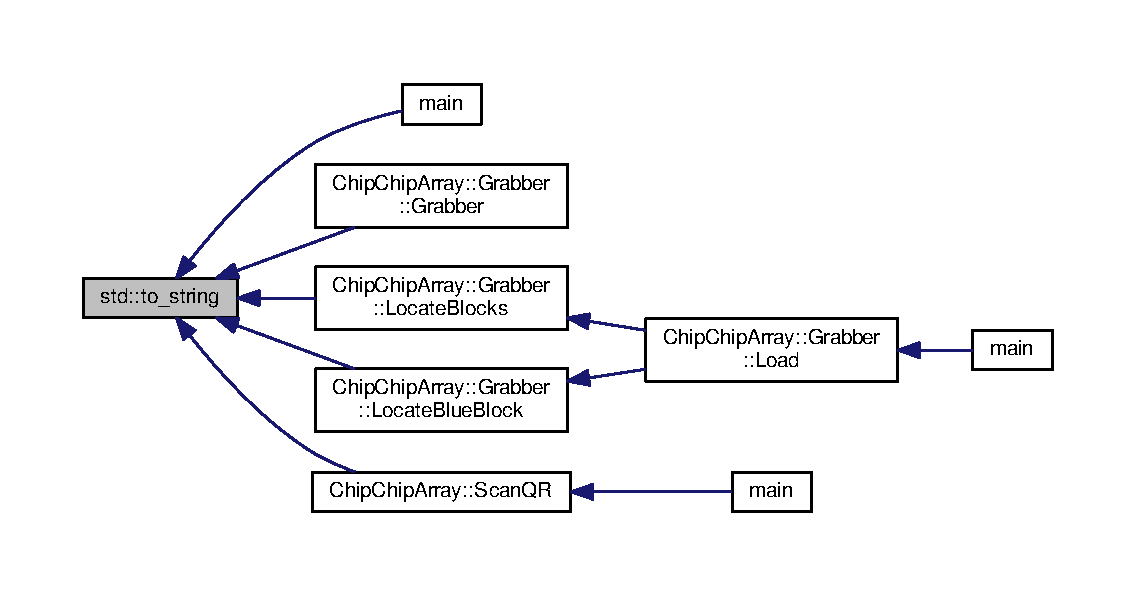
\includegraphics[width=350pt]{namespacestd_aa5ddf582a1c96ffe258c997be9a294a3_icgraph}
\end{center}
\end{figure}


\hypertarget{namespacestd_a6a0c3c323562edbd2f57da3d2bb74326}{\index{std@{std}!to\+\_\+string@{to\+\_\+string}}
\index{to\+\_\+string@{to\+\_\+string}!std@{std}}
\subsubsection[{to\+\_\+string}]{\setlength{\rightskip}{0pt plus 5cm}string std\+::to\+\_\+string (
\begin{DoxyParamCaption}
\item[{{\bf Color}}]{color}
\end{DoxyParamCaption}
)}}\label{namespacestd_a6a0c3c323562edbd2f57da3d2bb74326}
Converts a Color to a string. 

Definition at line 96 of file definitions.\+hpp.

\hypertarget{namespacestd_adb24d6df94a83c325573f7710df84953}{\index{std@{std}!to\+\_\+string@{to\+\_\+string}}
\index{to\+\_\+string@{to\+\_\+string}!std@{std}}
\subsubsection[{to\+\_\+string}]{\setlength{\rightskip}{0pt plus 5cm}string std\+::to\+\_\+string (
\begin{DoxyParamCaption}
\item[{{\bf Log\+Mode}}]{mode}
\end{DoxyParamCaption}
)}}\label{namespacestd_adb24d6df94a83c325573f7710df84953}
Converts a Log\+Mode to a string. 

Definition at line 123 of file definitions.\+hpp.

\hypertarget{namespacestd_a7fb649b1361ca7d95cc74045c0dadcdd}{\index{std@{std}!to\+\_\+string@{to\+\_\+string}}
\index{to\+\_\+string@{to\+\_\+string}!std@{std}}
\subsubsection[{to\+\_\+string}]{\setlength{\rightskip}{0pt plus 5cm}string std\+::to\+\_\+string (
\begin{DoxyParamCaption}
\item[{{\bf Result}}]{res}
\end{DoxyParamCaption}
)}}\label{namespacestd_a7fb649b1361ca7d95cc74045c0dadcdd}
Converts a Result to a string. 

Definition at line 131 of file definitions.\+hpp.

\hypertarget{namespacestd_aae21fd95009e4cc9fa25e1ad3830980b}{\index{std@{std}!to\+\_\+string@{to\+\_\+string}}
\index{to\+\_\+string@{to\+\_\+string}!std@{std}}
\subsubsection[{to\+\_\+string}]{\setlength{\rightskip}{0pt plus 5cm}string std\+::to\+\_\+string (
\begin{DoxyParamCaption}
\item[{{\bf Side}}]{side}
\end{DoxyParamCaption}
)}}\label{namespacestd_aae21fd95009e4cc9fa25e1ad3830980b}
Converts a Side to a string. 

Definition at line 158 of file definitions.\+hpp.

\hypertarget{namespacestd_a6bfcd2c3377165652c64085d7acb5c64}{\index{std@{std}!to\+\_\+string@{to\+\_\+string}}
\index{to\+\_\+string@{to\+\_\+string}!std@{std}}
\subsubsection[{to\+\_\+string}]{\setlength{\rightskip}{0pt plus 5cm}string std\+::to\+\_\+string (
\begin{DoxyParamCaption}
\item[{{\bf Size}}]{size}
\end{DoxyParamCaption}
)}}\label{namespacestd_a6bfcd2c3377165652c64085d7acb5c64}
Converts a Size to a string. 

Definition at line 166 of file definitions.\+hpp.

\hypertarget{namespacestd_ac50951e195256b4c2311f90189f64ba8}{\index{std@{std}!to\+\_\+string@{to\+\_\+string}}
\index{to\+\_\+string@{to\+\_\+string}!std@{std}}
\subsubsection[{to\+\_\+string}]{\setlength{\rightskip}{0pt plus 5cm}string std\+::to\+\_\+string (
\begin{DoxyParamCaption}
\item[{{\bf Zone}}]{zone}
\end{DoxyParamCaption}
)}}\label{namespacestd_ac50951e195256b4c2311f90189f64ba8}
Converts a Zone to a string. 

Definition at line 174 of file definitions.\+hpp.


\chapter{Class Documentation}
\hypertarget{classAdafruit__PWMServoDriver}{\section{Adafruit\+\_\+\+P\+W\+M\+Servo\+Driver Class Reference}
\label{classAdafruit__PWMServoDriver}\index{Adafruit\+\_\+\+P\+W\+M\+Servo\+Driver@{Adafruit\+\_\+\+P\+W\+M\+Servo\+Driver}}
}


{\ttfamily \#include $<$Adafruit\+\_\+\+P\+W\+M\+Servo\+Driver.\+h$>$}

\subsection*{Public Member Functions}
\begin{DoxyCompactItemize}
\item 
\hyperlink{classAdafruit__PWMServoDriver_a6a949db60836febbc61adef4cc5429ed}{Adafruit\+\_\+\+P\+W\+M\+Servo\+Driver} (\hyperlink{Servo__Position__Shell_8h_ab077fa1127453be2bd9d4c3c8a768fa7}{uint8\+\_\+t} addr=0x41)
\item 
void \hyperlink{classAdafruit__PWMServoDriver_aef401eaad3c34222ac916eb7bd936bc2}{begin} (void)
\item 
void \hyperlink{classAdafruit__PWMServoDriver_ac976f52233a75a4bd0eb6f2ce9b82b7f}{reset} (void)
\item 
void \hyperlink{classAdafruit__PWMServoDriver_a0ef6f1e3c81aebbd1d1da1bb12f3ed5c}{set\+P\+W\+M\+Freq} (float freq)
\item 
void \hyperlink{classAdafruit__PWMServoDriver_a724a7fc39c6fba34478ecc0eea038bd3}{set\+P\+W\+M} (\hyperlink{Servo__Position__Shell_8h_ab077fa1127453be2bd9d4c3c8a768fa7}{uint8\+\_\+t} num, \hyperlink{Adafruit__PWMServoDriver_8h_a395b3b2bf5cb4674ab41b6bda68c15bb}{uint16\+\_\+t} on, \hyperlink{Adafruit__PWMServoDriver_8h_a395b3b2bf5cb4674ab41b6bda68c15bb}{uint16\+\_\+t} off)
\item 
void \hyperlink{classAdafruit__PWMServoDriver_a1246cd50849fe0f068cc5d474e06ae96}{set\+Pin} (\hyperlink{Servo__Position__Shell_8h_ab077fa1127453be2bd9d4c3c8a768fa7}{uint8\+\_\+t} num, \hyperlink{Adafruit__PWMServoDriver_8h_a395b3b2bf5cb4674ab41b6bda68c15bb}{uint16\+\_\+t} val, bool invert=false)
\end{DoxyCompactItemize}


\subsection{Detailed Description}


Definition at line 65 of file Adafruit\+\_\+\+P\+W\+M\+Servo\+Driver.\+h.



\subsection{Constructor \& Destructor Documentation}
\hypertarget{classAdafruit__PWMServoDriver_a6a949db60836febbc61adef4cc5429ed}{\index{Adafruit\+\_\+\+P\+W\+M\+Servo\+Driver@{Adafruit\+\_\+\+P\+W\+M\+Servo\+Driver}!Adafruit\+\_\+\+P\+W\+M\+Servo\+Driver@{Adafruit\+\_\+\+P\+W\+M\+Servo\+Driver}}
\index{Adafruit\+\_\+\+P\+W\+M\+Servo\+Driver@{Adafruit\+\_\+\+P\+W\+M\+Servo\+Driver}!Adafruit\+\_\+\+P\+W\+M\+Servo\+Driver@{Adafruit\+\_\+\+P\+W\+M\+Servo\+Driver}}
\subsubsection[{Adafruit\+\_\+\+P\+W\+M\+Servo\+Driver}]{\setlength{\rightskip}{0pt plus 5cm}Adafruit\+\_\+\+P\+W\+M\+Servo\+Driver\+::\+Adafruit\+\_\+\+P\+W\+M\+Servo\+Driver (
\begin{DoxyParamCaption}
\item[{{\bf uint8\+\_\+t}}]{addr = {\ttfamily 0x41}}
\end{DoxyParamCaption}
)}}\label{classAdafruit__PWMServoDriver_a6a949db60836febbc61adef4cc5429ed}


Definition at line 29 of file Adafruit\+\_\+\+P\+W\+M\+Servo\+Driver.\+cpp.



\subsection{Member Function Documentation}
\hypertarget{classAdafruit__PWMServoDriver_aef401eaad3c34222ac916eb7bd936bc2}{\index{Adafruit\+\_\+\+P\+W\+M\+Servo\+Driver@{Adafruit\+\_\+\+P\+W\+M\+Servo\+Driver}!begin@{begin}}
\index{begin@{begin}!Adafruit\+\_\+\+P\+W\+M\+Servo\+Driver@{Adafruit\+\_\+\+P\+W\+M\+Servo\+Driver}}
\subsubsection[{begin}]{\setlength{\rightskip}{0pt plus 5cm}void Adafruit\+\_\+\+P\+W\+M\+Servo\+Driver\+::begin (
\begin{DoxyParamCaption}
\item[{void}]{}
\end{DoxyParamCaption}
)}}\label{classAdafruit__PWMServoDriver_aef401eaad3c34222ac916eb7bd936bc2}


Definition at line 34 of file Adafruit\+\_\+\+P\+W\+M\+Servo\+Driver.\+cpp.



Here is the call graph for this function\+:




Here is the caller graph for this function\+:


\hypertarget{classAdafruit__PWMServoDriver_ac976f52233a75a4bd0eb6f2ce9b82b7f}{\index{Adafruit\+\_\+\+P\+W\+M\+Servo\+Driver@{Adafruit\+\_\+\+P\+W\+M\+Servo\+Driver}!reset@{reset}}
\index{reset@{reset}!Adafruit\+\_\+\+P\+W\+M\+Servo\+Driver@{Adafruit\+\_\+\+P\+W\+M\+Servo\+Driver}}
\subsubsection[{reset}]{\setlength{\rightskip}{0pt plus 5cm}void Adafruit\+\_\+\+P\+W\+M\+Servo\+Driver\+::reset (
\begin{DoxyParamCaption}
\item[{void}]{}
\end{DoxyParamCaption}
)}}\label{classAdafruit__PWMServoDriver_ac976f52233a75a4bd0eb6f2ce9b82b7f}


Definition at line 42 of file Adafruit\+\_\+\+P\+W\+M\+Servo\+Driver.\+cpp.



Here is the caller graph for this function\+:


\hypertarget{classAdafruit__PWMServoDriver_a1246cd50849fe0f068cc5d474e06ae96}{\index{Adafruit\+\_\+\+P\+W\+M\+Servo\+Driver@{Adafruit\+\_\+\+P\+W\+M\+Servo\+Driver}!set\+Pin@{set\+Pin}}
\index{set\+Pin@{set\+Pin}!Adafruit\+\_\+\+P\+W\+M\+Servo\+Driver@{Adafruit\+\_\+\+P\+W\+M\+Servo\+Driver}}
\subsubsection[{set\+Pin}]{\setlength{\rightskip}{0pt plus 5cm}void Adafruit\+\_\+\+P\+W\+M\+Servo\+Driver\+::set\+Pin (
\begin{DoxyParamCaption}
\item[{{\bf uint8\+\_\+t}}]{num, }
\item[{{\bf uint16\+\_\+t}}]{val, }
\item[{bool}]{invert = {\ttfamily false}}
\end{DoxyParamCaption}
)}}\label{classAdafruit__PWMServoDriver_a1246cd50849fe0f068cc5d474e06ae96}


Definition at line 108 of file Adafruit\+\_\+\+P\+W\+M\+Servo\+Driver.\+cpp.



Here is the call graph for this function\+:


\hypertarget{classAdafruit__PWMServoDriver_a724a7fc39c6fba34478ecc0eea038bd3}{\index{Adafruit\+\_\+\+P\+W\+M\+Servo\+Driver@{Adafruit\+\_\+\+P\+W\+M\+Servo\+Driver}!set\+P\+W\+M@{set\+P\+W\+M}}
\index{set\+P\+W\+M@{set\+P\+W\+M}!Adafruit\+\_\+\+P\+W\+M\+Servo\+Driver@{Adafruit\+\_\+\+P\+W\+M\+Servo\+Driver}}
\subsubsection[{set\+P\+W\+M}]{\setlength{\rightskip}{0pt plus 5cm}void Adafruit\+\_\+\+P\+W\+M\+Servo\+Driver\+::set\+P\+W\+M (
\begin{DoxyParamCaption}
\item[{{\bf uint8\+\_\+t}}]{num, }
\item[{{\bf uint16\+\_\+t}}]{on, }
\item[{{\bf uint16\+\_\+t}}]{off}
\end{DoxyParamCaption}
)}}\label{classAdafruit__PWMServoDriver_a724a7fc39c6fba34478ecc0eea038bd3}


Definition at line 73 of file Adafruit\+\_\+\+P\+W\+M\+Servo\+Driver.\+cpp.



Here is the caller graph for this function\+:


\hypertarget{classAdafruit__PWMServoDriver_a0ef6f1e3c81aebbd1d1da1bb12f3ed5c}{\index{Adafruit\+\_\+\+P\+W\+M\+Servo\+Driver@{Adafruit\+\_\+\+P\+W\+M\+Servo\+Driver}!set\+P\+W\+M\+Freq@{set\+P\+W\+M\+Freq}}
\index{set\+P\+W\+M\+Freq@{set\+P\+W\+M\+Freq}!Adafruit\+\_\+\+P\+W\+M\+Servo\+Driver@{Adafruit\+\_\+\+P\+W\+M\+Servo\+Driver}}
\subsubsection[{set\+P\+W\+M\+Freq}]{\setlength{\rightskip}{0pt plus 5cm}void Adafruit\+\_\+\+P\+W\+M\+Servo\+Driver\+::set\+P\+W\+M\+Freq (
\begin{DoxyParamCaption}
\item[{float}]{freq}
\end{DoxyParamCaption}
)}}\label{classAdafruit__PWMServoDriver_a0ef6f1e3c81aebbd1d1da1bb12f3ed5c}


Definition at line 46 of file Adafruit\+\_\+\+P\+W\+M\+Servo\+Driver.\+cpp.



Here is the caller graph for this function\+:




The documentation for this class was generated from the following files\+:\begin{DoxyCompactItemize}
\item 
src/\hyperlink{Adafruit__PWMServoDriver_8h}{Adafruit\+\_\+\+P\+W\+M\+Servo\+Driver.\+h}\item 
src/\hyperlink{Adafruit__PWMServoDriver_8cpp}{Adafruit\+\_\+\+P\+W\+M\+Servo\+Driver.\+cpp}\end{DoxyCompactItemize}

\hypertarget{classChipChipArray_1_1Arm}{\section{Chip\+Chip\+Array\+:\+:Arm Class Reference}
\label{classChipChipArray_1_1Arm}\index{Chip\+Chip\+Array\+::\+Arm@{Chip\+Chip\+Array\+::\+Arm}}
}


{\ttfamily \#include $<$Arm.\+hpp$>$}

\subsection*{Public Member Functions}
\begin{DoxyCompactItemize}
\item 
\hyperlink{classChipChipArray_1_1Arm_aeda43d8461e50eaca9aa891ee2863c05}{Arm} ()
\item 
void \hyperlink{classChipChipArray_1_1Arm_a8b077a3791d9fc5ef285c1520fe4c5d8}{Base\+Tilt} (\hyperlink{definitions_8hpp_adde6aaee8457bee49c2a92621fe22b79}{uint8} a)
\item 
void \hyperlink{classChipChipArray_1_1Arm_addaedfe85ff2b14ff00c344fc4b40cd6}{Base\+Turn} (\hyperlink{definitions_8hpp_adde6aaee8457bee49c2a92621fe22b79}{uint8} a)
\item 
void \hyperlink{classChipChipArray_1_1Arm_af84b91c664baec0f2882dcf4089ae027}{d\+Base\+Tilt} (\hyperlink{definitions_8hpp_a74df79fde3c518e55b29ce6360a9c76e}{sint16} a)
\item 
void \hyperlink{classChipChipArray_1_1Arm_a980f5bd278cbe06aa21754fb8e0324b3}{d\+Base\+Turn} (\hyperlink{definitions_8hpp_a74df79fde3c518e55b29ce6360a9c76e}{sint16} a)
\item 
void \hyperlink{classChipChipArray_1_1Arm_ae8d0a664dd1a0e556cf40c0984035163}{d\+Elbow} (\hyperlink{definitions_8hpp_a74df79fde3c518e55b29ce6360a9c76e}{sint16} a)
\item 
void \hyperlink{classChipChipArray_1_1Arm_a2e46473723c15e88952a2c4fbd0a8bd8}{d\+Grippers} (\hyperlink{definitions_8hpp_a74df79fde3c518e55b29ce6360a9c76e}{sint16} a)
\item 
void \hyperlink{classChipChipArray_1_1Arm_a43daba698f13a522887ad022b78557bb}{d\+Wrist\+Tilt} (\hyperlink{definitions_8hpp_a74df79fde3c518e55b29ce6360a9c76e}{sint16} a)
\item 
void \hyperlink{classChipChipArray_1_1Arm_a6bde822b1be63926e21222f36aad67b3}{d\+Wrist\+Twist} (\hyperlink{definitions_8hpp_a74df79fde3c518e55b29ce6360a9c76e}{sint16} a)
\item 
void \hyperlink{classChipChipArray_1_1Arm_ac45149e03abfac230b75156bb42e8417}{Elbow} (\hyperlink{definitions_8hpp_adde6aaee8457bee49c2a92621fe22b79}{uint8} a)
\item 
void \hyperlink{classChipChipArray_1_1Arm_afe581f2e6c85ba07729d3ffe90fee9cd}{Grippers} (\hyperlink{definitions_8hpp_adde6aaee8457bee49c2a92621fe22b79}{uint8} a)
\item 
void \hyperlink{classChipChipArray_1_1Arm_a8871580fd6a75fd60d99300f2b5c21d1}{Hover} (\hyperlink{definitions_8hpp_adbd1e7a33d3e1751c7b2aa2562d0ecb9}{Zone} zone)
\item 
void \hyperlink{classChipChipArray_1_1Arm_ad61f7c1e63eb09981b6c304bd924e217}{Wrist\+Tilt} (\hyperlink{definitions_8hpp_adde6aaee8457bee49c2a92621fe22b79}{uint8} a)
\item 
void \hyperlink{classChipChipArray_1_1Arm_a35ec7756840d9d32dcfbb88d831f087f}{Wrist\+Twist} (\hyperlink{definitions_8hpp_adde6aaee8457bee49c2a92621fe22b79}{uint8} a)
\end{DoxyCompactItemize}
\subsection*{Protected Member Functions}
\begin{DoxyCompactItemize}
\item 
void \hyperlink{classChipChipArray_1_1Arm_a6da0950c7e3bd4a31264e562916c032d}{d\+Left\+Gripper} (\hyperlink{definitions_8hpp_a74df79fde3c518e55b29ce6360a9c76e}{sint16} a)
\item 
void \hyperlink{classChipChipArray_1_1Arm_adfa7cc779b7ec3bf8453277796c142ed}{d\+Right\+Gripper} (\hyperlink{definitions_8hpp_a74df79fde3c518e55b29ce6360a9c76e}{sint16} a)
\item 
void \hyperlink{classChipChipArray_1_1Arm_a776eade3a7aaa6effaabad7f37c71031}{Left\+Gripper} (\hyperlink{definitions_8hpp_adde6aaee8457bee49c2a92621fe22b79}{uint8} a)
\item 
void \hyperlink{classChipChipArray_1_1Arm_a46a0b0cfb37cb0b663c91cd07e440e10}{Right\+Gripper} (\hyperlink{definitions_8hpp_adde6aaee8457bee49c2a92621fe22b79}{uint8} a)
\end{DoxyCompactItemize}
\subsection*{Protected Attributes}
\begin{DoxyCompactItemize}
\item 
\hyperlink{definitions_8hpp_adde6aaee8457bee49c2a92621fe22b79}{uint8} \hyperlink{classChipChipArray_1_1Arm_abe425c250c1929e9c9c86e6ea9eeeb04}{servo\+Pos} = \{ 0, 0, 0, 0, 0, 0, 0 \}
\end{DoxyCompactItemize}


\subsection{Detailed Description}
This class provides a layer of abstraction from the existing servo interface. It is designed to make more sense programmatically and to be easier to use. 

Definition at line 19 of file Arm.\+hpp.



\subsection{Constructor \& Destructor Documentation}
\hypertarget{classChipChipArray_1_1Arm_aeda43d8461e50eaca9aa891ee2863c05}{\index{Chip\+Chip\+Array\+::\+Arm@{Chip\+Chip\+Array\+::\+Arm}!Arm@{Arm}}
\index{Arm@{Arm}!Chip\+Chip\+Array\+::\+Arm@{Chip\+Chip\+Array\+::\+Arm}}
\subsubsection[{Arm}]{\setlength{\rightskip}{0pt plus 5cm}Chip\+Chip\+Array\+::\+Arm\+::\+Arm (
\begin{DoxyParamCaption}
{}
\end{DoxyParamCaption}
)}}\label{classChipChipArray_1_1Arm_aeda43d8461e50eaca9aa891ee2863c05}
Initializes the I2\+C interface for the arm if another instance of the \hyperlink{classChipChipArray_1_1Arm}{Arm} class has not already. 

Definition at line 174 of file Arm.\+hpp.



Here is the call graph for this function\+:
\nopagebreak
\begin{figure}[H]
\begin{center}
\leavevmode
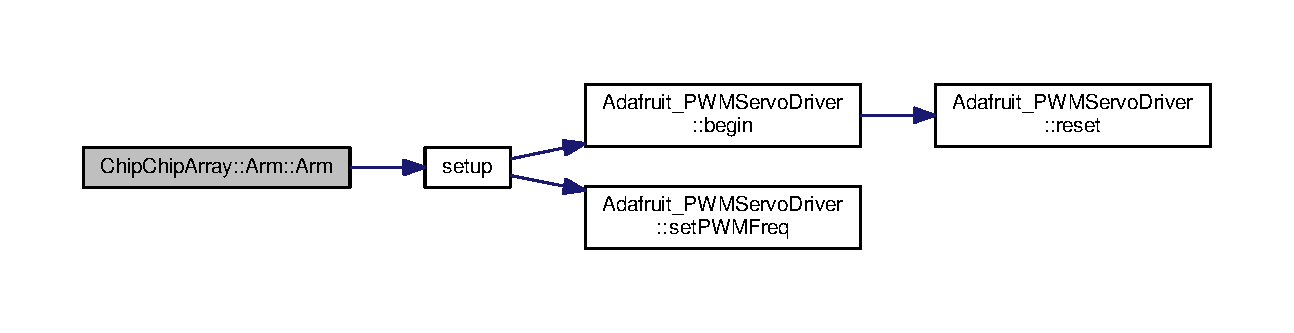
\includegraphics[width=350pt]{classChipChipArray_1_1Arm_aeda43d8461e50eaca9aa891ee2863c05_cgraph}
\end{center}
\end{figure}




\subsection{Member Function Documentation}
\hypertarget{classChipChipArray_1_1Arm_a8b077a3791d9fc5ef285c1520fe4c5d8}{\index{Chip\+Chip\+Array\+::\+Arm@{Chip\+Chip\+Array\+::\+Arm}!Base\+Tilt@{Base\+Tilt}}
\index{Base\+Tilt@{Base\+Tilt}!Chip\+Chip\+Array\+::\+Arm@{Chip\+Chip\+Array\+::\+Arm}}
\subsubsection[{Base\+Tilt}]{\setlength{\rightskip}{0pt plus 5cm}void Chip\+Chip\+Array\+::\+Arm\+::\+Base\+Tilt (
\begin{DoxyParamCaption}
\item[{{\bf uint8}}]{a}
\end{DoxyParamCaption}
)}}\label{classChipChipArray_1_1Arm_a8b077a3791d9fc5ef285c1520fe4c5d8}
Tilts the base of the arm.


\begin{DoxyParams}{Parameters}
{\em a} & desired servo position in degrees \\
\hline
\end{DoxyParams}


Definition at line 181 of file Arm.\+hpp.



Here is the call graph for this function\+:
\nopagebreak
\begin{figure}[H]
\begin{center}
\leavevmode
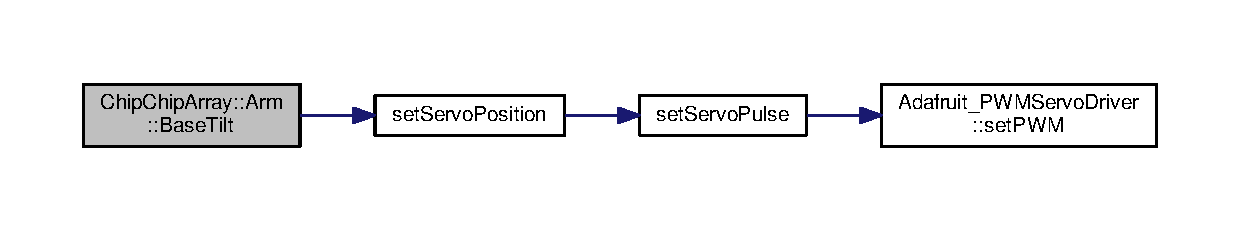
\includegraphics[width=350pt]{classChipChipArray_1_1Arm_a8b077a3791d9fc5ef285c1520fe4c5d8_cgraph}
\end{center}
\end{figure}


\hypertarget{classChipChipArray_1_1Arm_addaedfe85ff2b14ff00c344fc4b40cd6}{\index{Chip\+Chip\+Array\+::\+Arm@{Chip\+Chip\+Array\+::\+Arm}!Base\+Turn@{Base\+Turn}}
\index{Base\+Turn@{Base\+Turn}!Chip\+Chip\+Array\+::\+Arm@{Chip\+Chip\+Array\+::\+Arm}}
\subsubsection[{Base\+Turn}]{\setlength{\rightskip}{0pt plus 5cm}void Chip\+Chip\+Array\+::\+Arm\+::\+Base\+Turn (
\begin{DoxyParamCaption}
\item[{{\bf uint8}}]{a}
\end{DoxyParamCaption}
)}}\label{classChipChipArray_1_1Arm_addaedfe85ff2b14ff00c344fc4b40cd6}
Twists the entire arm.


\begin{DoxyParams}{Parameters}
{\em a} & desired servo position in degrees \\
\hline
\end{DoxyParams}


Definition at line 186 of file Arm.\+hpp.



Here is the call graph for this function\+:
\nopagebreak
\begin{figure}[H]
\begin{center}
\leavevmode
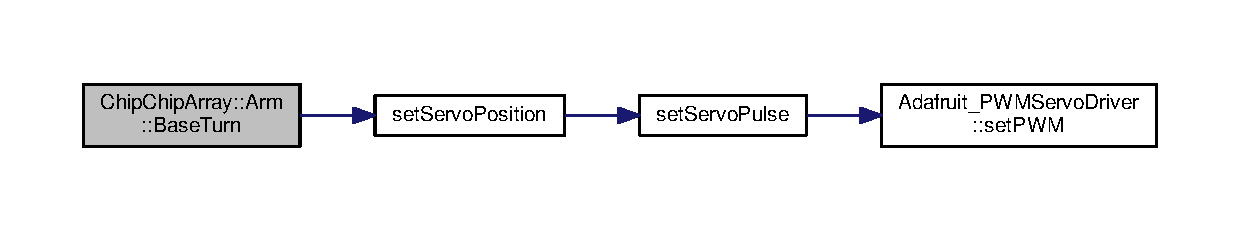
\includegraphics[width=350pt]{classChipChipArray_1_1Arm_addaedfe85ff2b14ff00c344fc4b40cd6_cgraph}
\end{center}
\end{figure}


\hypertarget{classChipChipArray_1_1Arm_af84b91c664baec0f2882dcf4089ae027}{\index{Chip\+Chip\+Array\+::\+Arm@{Chip\+Chip\+Array\+::\+Arm}!d\+Base\+Tilt@{d\+Base\+Tilt}}
\index{d\+Base\+Tilt@{d\+Base\+Tilt}!Chip\+Chip\+Array\+::\+Arm@{Chip\+Chip\+Array\+::\+Arm}}
\subsubsection[{d\+Base\+Tilt}]{\setlength{\rightskip}{0pt plus 5cm}void Chip\+Chip\+Array\+::\+Arm\+::d\+Base\+Tilt (
\begin{DoxyParamCaption}
\item[{{\bf sint16}}]{a}
\end{DoxyParamCaption}
)}}\label{classChipChipArray_1_1Arm_af84b91c664baec0f2882dcf4089ae027}
Tilts the base a certain number of degrees.


\begin{DoxyParams}{Parameters}
{\em degrees} & to move servo. Positive values add to the servo angle, and negative values subtract from the servo angle. \\
\hline
\end{DoxyParams}


Definition at line 191 of file Arm.\+hpp.



Here is the call graph for this function\+:
\nopagebreak
\begin{figure}[H]
\begin{center}
\leavevmode
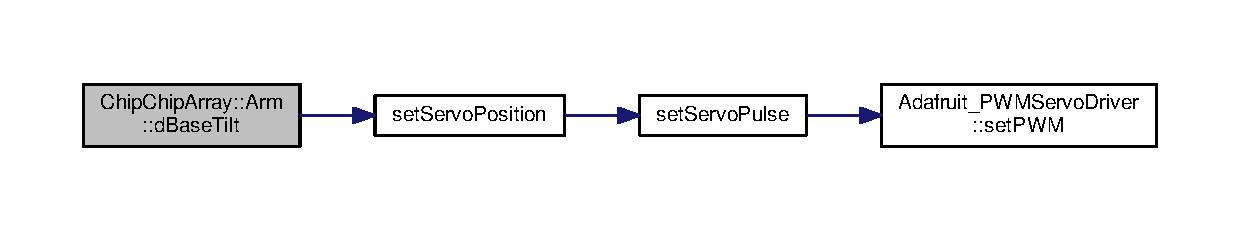
\includegraphics[width=350pt]{classChipChipArray_1_1Arm_af84b91c664baec0f2882dcf4089ae027_cgraph}
\end{center}
\end{figure}


\hypertarget{classChipChipArray_1_1Arm_a980f5bd278cbe06aa21754fb8e0324b3}{\index{Chip\+Chip\+Array\+::\+Arm@{Chip\+Chip\+Array\+::\+Arm}!d\+Base\+Turn@{d\+Base\+Turn}}
\index{d\+Base\+Turn@{d\+Base\+Turn}!Chip\+Chip\+Array\+::\+Arm@{Chip\+Chip\+Array\+::\+Arm}}
\subsubsection[{d\+Base\+Turn}]{\setlength{\rightskip}{0pt plus 5cm}void Chip\+Chip\+Array\+::\+Arm\+::d\+Base\+Turn (
\begin{DoxyParamCaption}
\item[{{\bf sint16}}]{a}
\end{DoxyParamCaption}
)}}\label{classChipChipArray_1_1Arm_a980f5bd278cbe06aa21754fb8e0324b3}
Turn the base a certain number of degrees.


\begin{DoxyParams}{Parameters}
{\em degrees} & to move servo. Positive values add to the servo angle, and negative values subtract from the servo angle. \\
\hline
\end{DoxyParams}


Definition at line 197 of file Arm.\+hpp.



Here is the call graph for this function\+:
\nopagebreak
\begin{figure}[H]
\begin{center}
\leavevmode
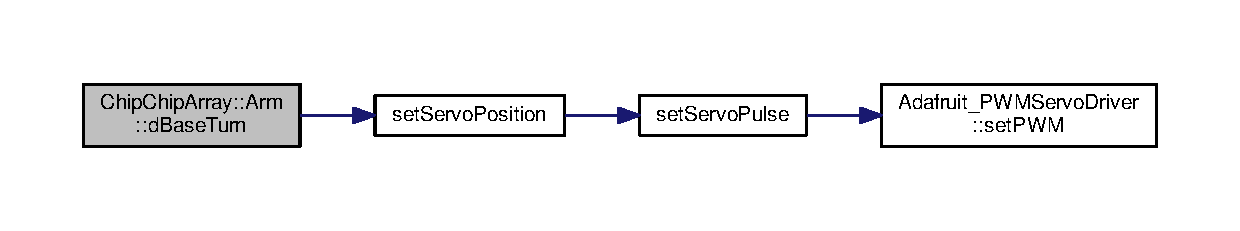
\includegraphics[width=350pt]{classChipChipArray_1_1Arm_a980f5bd278cbe06aa21754fb8e0324b3_cgraph}
\end{center}
\end{figure}


\hypertarget{classChipChipArray_1_1Arm_ae8d0a664dd1a0e556cf40c0984035163}{\index{Chip\+Chip\+Array\+::\+Arm@{Chip\+Chip\+Array\+::\+Arm}!d\+Elbow@{d\+Elbow}}
\index{d\+Elbow@{d\+Elbow}!Chip\+Chip\+Array\+::\+Arm@{Chip\+Chip\+Array\+::\+Arm}}
\subsubsection[{d\+Elbow}]{\setlength{\rightskip}{0pt plus 5cm}void Chip\+Chip\+Array\+::\+Arm\+::d\+Elbow (
\begin{DoxyParamCaption}
\item[{{\bf sint16}}]{a}
\end{DoxyParamCaption}
)}}\label{classChipChipArray_1_1Arm_ae8d0a664dd1a0e556cf40c0984035163}
Bend the elbow a certain number of degrees.


\begin{DoxyParams}{Parameters}
{\em degrees} & to move servo. Positive values add to the servo angle, and negative values subtract from the servo angle. \\
\hline
\end{DoxyParams}


Definition at line 203 of file Arm.\+hpp.



Here is the call graph for this function\+:
\nopagebreak
\begin{figure}[H]
\begin{center}
\leavevmode
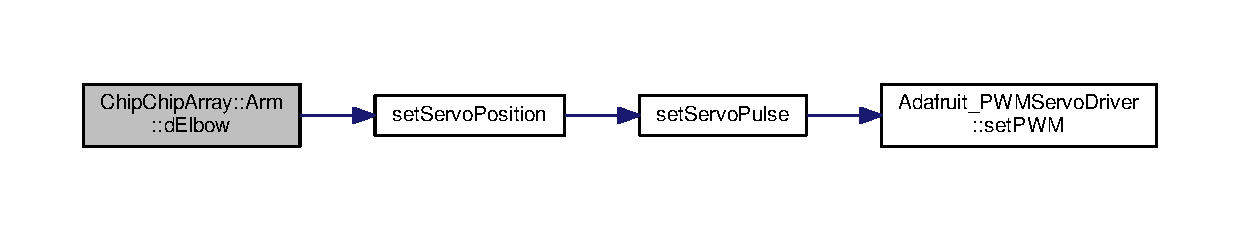
\includegraphics[width=350pt]{classChipChipArray_1_1Arm_ae8d0a664dd1a0e556cf40c0984035163_cgraph}
\end{center}
\end{figure}


\hypertarget{classChipChipArray_1_1Arm_a2e46473723c15e88952a2c4fbd0a8bd8}{\index{Chip\+Chip\+Array\+::\+Arm@{Chip\+Chip\+Array\+::\+Arm}!d\+Grippers@{d\+Grippers}}
\index{d\+Grippers@{d\+Grippers}!Chip\+Chip\+Array\+::\+Arm@{Chip\+Chip\+Array\+::\+Arm}}
\subsubsection[{d\+Grippers}]{\setlength{\rightskip}{0pt plus 5cm}void Chip\+Chip\+Array\+::\+Arm\+::d\+Grippers (
\begin{DoxyParamCaption}
\item[{{\bf sint16}}]{a}
\end{DoxyParamCaption}
)}}\label{classChipChipArray_1_1Arm_a2e46473723c15e88952a2c4fbd0a8bd8}
Move the grippers a certain number of degrees. Note that they will both move inward or outward; one will never move inward and the other outward.


\begin{DoxyParams}{Parameters}
{\em degrees} & to move servo. \\
\hline
\end{DoxyParams}


Definition at line 209 of file Arm.\+hpp.

\hypertarget{classChipChipArray_1_1Arm_a6da0950c7e3bd4a31264e562916c032d}{\index{Chip\+Chip\+Array\+::\+Arm@{Chip\+Chip\+Array\+::\+Arm}!d\+Left\+Gripper@{d\+Left\+Gripper}}
\index{d\+Left\+Gripper@{d\+Left\+Gripper}!Chip\+Chip\+Array\+::\+Arm@{Chip\+Chip\+Array\+::\+Arm}}
\subsubsection[{d\+Left\+Gripper}]{\setlength{\rightskip}{0pt plus 5cm}void Chip\+Chip\+Array\+::\+Arm\+::d\+Left\+Gripper (
\begin{DoxyParamCaption}
\item[{{\bf sint16}}]{a}
\end{DoxyParamCaption}
)\hspace{0.3cm}{\ttfamily [protected]}}}\label{classChipChipArray_1_1Arm_a6da0950c7e3bd4a31264e562916c032d}
Moves the left gripper servo a certain number of degrees.


\begin{DoxyParams}{Parameters}
{\em degrees} & to move servo. Positive values add to the servo angle, and negative values subtract from the servo angle. \\
\hline
\end{DoxyParams}


Definition at line 216 of file Arm.\+hpp.



Here is the call graph for this function\+:
\nopagebreak
\begin{figure}[H]
\begin{center}
\leavevmode
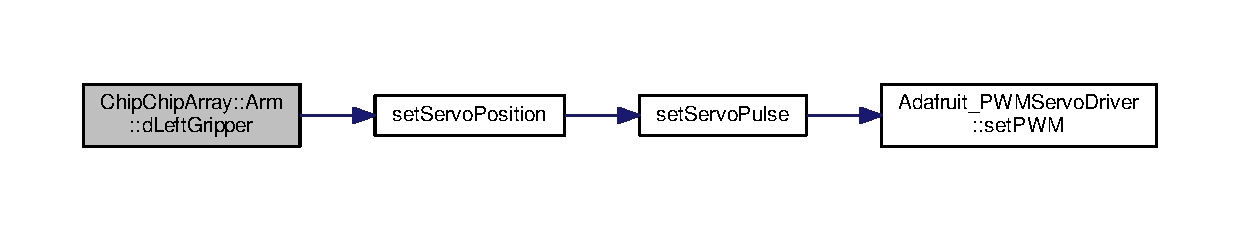
\includegraphics[width=350pt]{classChipChipArray_1_1Arm_a6da0950c7e3bd4a31264e562916c032d_cgraph}
\end{center}
\end{figure}


\hypertarget{classChipChipArray_1_1Arm_adfa7cc779b7ec3bf8453277796c142ed}{\index{Chip\+Chip\+Array\+::\+Arm@{Chip\+Chip\+Array\+::\+Arm}!d\+Right\+Gripper@{d\+Right\+Gripper}}
\index{d\+Right\+Gripper@{d\+Right\+Gripper}!Chip\+Chip\+Array\+::\+Arm@{Chip\+Chip\+Array\+::\+Arm}}
\subsubsection[{d\+Right\+Gripper}]{\setlength{\rightskip}{0pt plus 5cm}void Chip\+Chip\+Array\+::\+Arm\+::d\+Right\+Gripper (
\begin{DoxyParamCaption}
\item[{{\bf sint16}}]{a}
\end{DoxyParamCaption}
)\hspace{0.3cm}{\ttfamily [protected]}}}\label{classChipChipArray_1_1Arm_adfa7cc779b7ec3bf8453277796c142ed}
Moves the right gripper servo a certain number of degrees.


\begin{DoxyParams}{Parameters}
{\em degrees} & to move servo. Positive values add to the servo angle, and negative values subtract from the servo angle. \\
\hline
\end{DoxyParams}


Definition at line 222 of file Arm.\+hpp.



Here is the call graph for this function\+:
\nopagebreak
\begin{figure}[H]
\begin{center}
\leavevmode
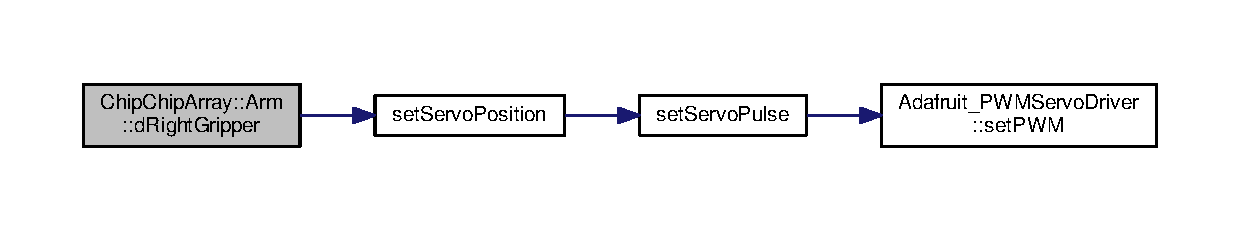
\includegraphics[width=350pt]{classChipChipArray_1_1Arm_adfa7cc779b7ec3bf8453277796c142ed_cgraph}
\end{center}
\end{figure}


\hypertarget{classChipChipArray_1_1Arm_a43daba698f13a522887ad022b78557bb}{\index{Chip\+Chip\+Array\+::\+Arm@{Chip\+Chip\+Array\+::\+Arm}!d\+Wrist\+Tilt@{d\+Wrist\+Tilt}}
\index{d\+Wrist\+Tilt@{d\+Wrist\+Tilt}!Chip\+Chip\+Array\+::\+Arm@{Chip\+Chip\+Array\+::\+Arm}}
\subsubsection[{d\+Wrist\+Tilt}]{\setlength{\rightskip}{0pt plus 5cm}void Chip\+Chip\+Array\+::\+Arm\+::d\+Wrist\+Tilt (
\begin{DoxyParamCaption}
\item[{{\bf sint16}}]{a}
\end{DoxyParamCaption}
)}}\label{classChipChipArray_1_1Arm_a43daba698f13a522887ad022b78557bb}
Tilt the wrist a certain number of degrees.


\begin{DoxyParams}{Parameters}
{\em degrees} & to move servo. Positive values add to the servo angle, and negative values subtract from the servo angle. \\
\hline
\end{DoxyParams}


Definition at line 228 of file Arm.\+hpp.



Here is the call graph for this function\+:
\nopagebreak
\begin{figure}[H]
\begin{center}
\leavevmode
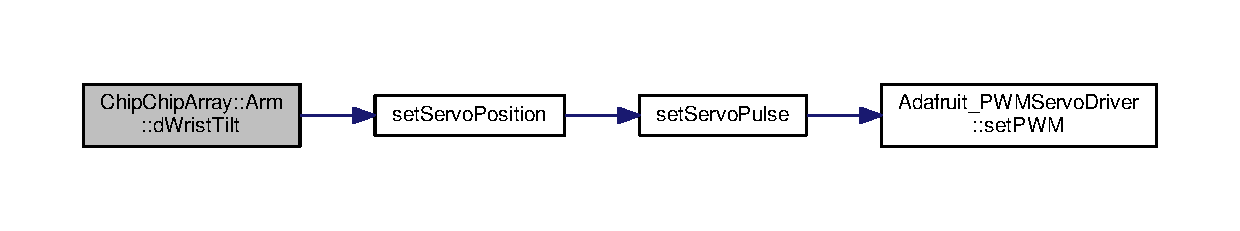
\includegraphics[width=350pt]{classChipChipArray_1_1Arm_a43daba698f13a522887ad022b78557bb_cgraph}
\end{center}
\end{figure}


\hypertarget{classChipChipArray_1_1Arm_a6bde822b1be63926e21222f36aad67b3}{\index{Chip\+Chip\+Array\+::\+Arm@{Chip\+Chip\+Array\+::\+Arm}!d\+Wrist\+Twist@{d\+Wrist\+Twist}}
\index{d\+Wrist\+Twist@{d\+Wrist\+Twist}!Chip\+Chip\+Array\+::\+Arm@{Chip\+Chip\+Array\+::\+Arm}}
\subsubsection[{d\+Wrist\+Twist}]{\setlength{\rightskip}{0pt plus 5cm}void Chip\+Chip\+Array\+::\+Arm\+::d\+Wrist\+Twist (
\begin{DoxyParamCaption}
\item[{{\bf sint16}}]{a}
\end{DoxyParamCaption}
)}}\label{classChipChipArray_1_1Arm_a6bde822b1be63926e21222f36aad67b3}
Twist the wrist a certain number of degrees.


\begin{DoxyParams}{Parameters}
{\em degrees} & to move servo. Positive values add to the servo angle, and negative values subtract from the servo angle. \\
\hline
\end{DoxyParams}
\hypertarget{classChipChipArray_1_1Arm_ac45149e03abfac230b75156bb42e8417}{\index{Chip\+Chip\+Array\+::\+Arm@{Chip\+Chip\+Array\+::\+Arm}!Elbow@{Elbow}}
\index{Elbow@{Elbow}!Chip\+Chip\+Array\+::\+Arm@{Chip\+Chip\+Array\+::\+Arm}}
\subsubsection[{Elbow}]{\setlength{\rightskip}{0pt plus 5cm}void Chip\+Chip\+Array\+::\+Arm\+::\+Elbow (
\begin{DoxyParamCaption}
\item[{{\bf uint8}}]{a}
\end{DoxyParamCaption}
)}}\label{classChipChipArray_1_1Arm_ac45149e03abfac230b75156bb42e8417}
Bend the elbow to a specific position.


\begin{DoxyParams}{Parameters}
{\em a} & desired servo position in degrees \\
\hline
\end{DoxyParams}


Definition at line 240 of file Arm.\+hpp.



Here is the call graph for this function\+:
\nopagebreak
\begin{figure}[H]
\begin{center}
\leavevmode
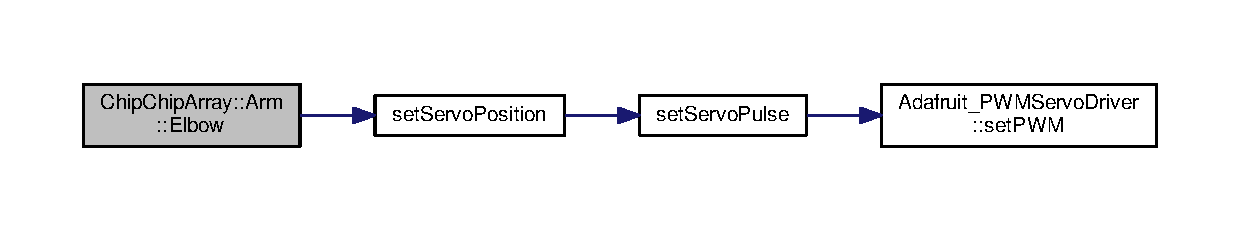
\includegraphics[width=350pt]{classChipChipArray_1_1Arm_ac45149e03abfac230b75156bb42e8417_cgraph}
\end{center}
\end{figure}


\hypertarget{classChipChipArray_1_1Arm_afe581f2e6c85ba07729d3ffe90fee9cd}{\index{Chip\+Chip\+Array\+::\+Arm@{Chip\+Chip\+Array\+::\+Arm}!Grippers@{Grippers}}
\index{Grippers@{Grippers}!Chip\+Chip\+Array\+::\+Arm@{Chip\+Chip\+Array\+::\+Arm}}
\subsubsection[{Grippers}]{\setlength{\rightskip}{0pt plus 5cm}void Chip\+Chip\+Array\+::\+Arm\+::\+Grippers (
\begin{DoxyParamCaption}
\item[{{\bf uint8}}]{a}
\end{DoxyParamCaption}
)}}\label{classChipChipArray_1_1Arm_afe581f2e6c85ba07729d3ffe90fee9cd}
Move the grippers to a specific position. Note that they will both move inward or outward; one will never move inward and the other outward.


\begin{DoxyParams}{Parameters}
{\em a} & desired servo position in degrees \\
\hline
\end{DoxyParams}


Definition at line 245 of file Arm.\+hpp.

\hypertarget{classChipChipArray_1_1Arm_a8871580fd6a75fd60d99300f2b5c21d1}{\index{Chip\+Chip\+Array\+::\+Arm@{Chip\+Chip\+Array\+::\+Arm}!Hover@{Hover}}
\index{Hover@{Hover}!Chip\+Chip\+Array\+::\+Arm@{Chip\+Chip\+Array\+::\+Arm}}
\subsubsection[{Hover}]{\setlength{\rightskip}{0pt plus 5cm}void Chip\+Chip\+Array\+::\+Arm\+::\+Hover (
\begin{DoxyParamCaption}
\item[{{\bf Zone}}]{zone}
\end{DoxyParamCaption}
)}}\label{classChipChipArray_1_1Arm_a8871580fd6a75fd60d99300f2b5c21d1}
Moves arm into its \char`\"{}hovering\char`\"{} position over the blocks. The position changes with the zone.


\begin{DoxyParams}{Parameters}
{\em zone} & the zone for which the arm should position itself \\
\hline
\end{DoxyParams}


Definition at line 249 of file Arm.\+hpp.

\hypertarget{classChipChipArray_1_1Arm_a776eade3a7aaa6effaabad7f37c71031}{\index{Chip\+Chip\+Array\+::\+Arm@{Chip\+Chip\+Array\+::\+Arm}!Left\+Gripper@{Left\+Gripper}}
\index{Left\+Gripper@{Left\+Gripper}!Chip\+Chip\+Array\+::\+Arm@{Chip\+Chip\+Array\+::\+Arm}}
\subsubsection[{Left\+Gripper}]{\setlength{\rightskip}{0pt plus 5cm}void Chip\+Chip\+Array\+::\+Arm\+::\+Left\+Gripper (
\begin{DoxyParamCaption}
\item[{{\bf uint8}}]{a}
\end{DoxyParamCaption}
)\hspace{0.3cm}{\ttfamily [protected]}}}\label{classChipChipArray_1_1Arm_a776eade3a7aaa6effaabad7f37c71031}
Moves the left gripper to a specific position.


\begin{DoxyParams}{Parameters}
{\em a} & desired servo position in degrees \\
\hline
\end{DoxyParams}


Definition at line 253 of file Arm.\+hpp.



Here is the call graph for this function\+:
\nopagebreak
\begin{figure}[H]
\begin{center}
\leavevmode
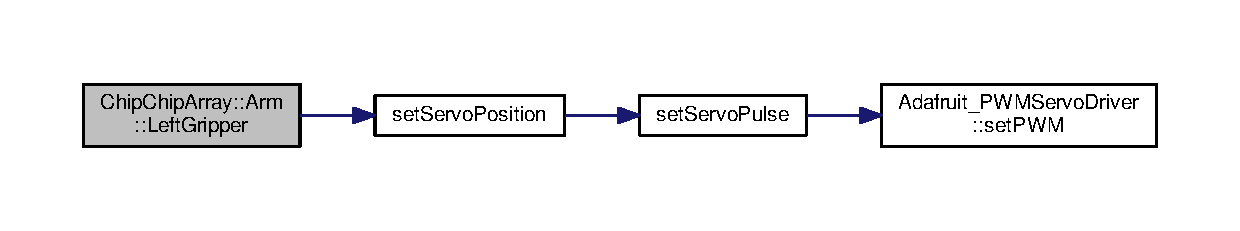
\includegraphics[width=350pt]{classChipChipArray_1_1Arm_a776eade3a7aaa6effaabad7f37c71031_cgraph}
\end{center}
\end{figure}


\hypertarget{classChipChipArray_1_1Arm_a46a0b0cfb37cb0b663c91cd07e440e10}{\index{Chip\+Chip\+Array\+::\+Arm@{Chip\+Chip\+Array\+::\+Arm}!Right\+Gripper@{Right\+Gripper}}
\index{Right\+Gripper@{Right\+Gripper}!Chip\+Chip\+Array\+::\+Arm@{Chip\+Chip\+Array\+::\+Arm}}
\subsubsection[{Right\+Gripper}]{\setlength{\rightskip}{0pt plus 5cm}void Chip\+Chip\+Array\+::\+Arm\+::\+Right\+Gripper (
\begin{DoxyParamCaption}
\item[{{\bf uint8}}]{a}
\end{DoxyParamCaption}
)\hspace{0.3cm}{\ttfamily [protected]}}}\label{classChipChipArray_1_1Arm_a46a0b0cfb37cb0b663c91cd07e440e10}
Moves the right gripper to a specific position.


\begin{DoxyParams}{Parameters}
{\em a} & desired servo position in degrees \\
\hline
\end{DoxyParams}


Definition at line 258 of file Arm.\+hpp.



Here is the call graph for this function\+:
\nopagebreak
\begin{figure}[H]
\begin{center}
\leavevmode
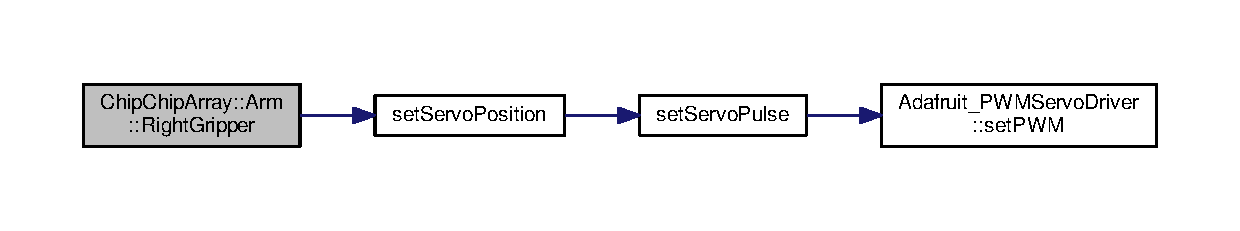
\includegraphics[width=350pt]{classChipChipArray_1_1Arm_a46a0b0cfb37cb0b663c91cd07e440e10_cgraph}
\end{center}
\end{figure}


\hypertarget{classChipChipArray_1_1Arm_ad61f7c1e63eb09981b6c304bd924e217}{\index{Chip\+Chip\+Array\+::\+Arm@{Chip\+Chip\+Array\+::\+Arm}!Wrist\+Tilt@{Wrist\+Tilt}}
\index{Wrist\+Tilt@{Wrist\+Tilt}!Chip\+Chip\+Array\+::\+Arm@{Chip\+Chip\+Array\+::\+Arm}}
\subsubsection[{Wrist\+Tilt}]{\setlength{\rightskip}{0pt plus 5cm}void Chip\+Chip\+Array\+::\+Arm\+::\+Wrist\+Tilt (
\begin{DoxyParamCaption}
\item[{{\bf uint8}}]{a}
\end{DoxyParamCaption}
)}}\label{classChipChipArray_1_1Arm_ad61f7c1e63eb09981b6c304bd924e217}
Tilt the wrist to a specific position.


\begin{DoxyParams}{Parameters}
{\em a} & desired servo position in degrees \\
\hline
\end{DoxyParams}


Definition at line 263 of file Arm.\+hpp.



Here is the call graph for this function\+:
\nopagebreak
\begin{figure}[H]
\begin{center}
\leavevmode
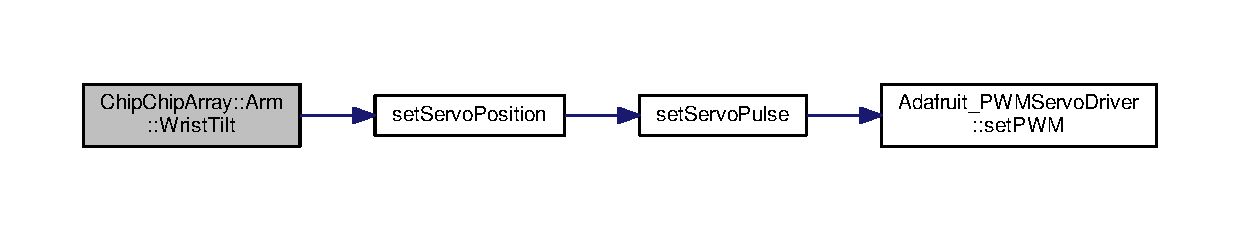
\includegraphics[width=350pt]{classChipChipArray_1_1Arm_ad61f7c1e63eb09981b6c304bd924e217_cgraph}
\end{center}
\end{figure}


\hypertarget{classChipChipArray_1_1Arm_a35ec7756840d9d32dcfbb88d831f087f}{\index{Chip\+Chip\+Array\+::\+Arm@{Chip\+Chip\+Array\+::\+Arm}!Wrist\+Twist@{Wrist\+Twist}}
\index{Wrist\+Twist@{Wrist\+Twist}!Chip\+Chip\+Array\+::\+Arm@{Chip\+Chip\+Array\+::\+Arm}}
\subsubsection[{Wrist\+Twist}]{\setlength{\rightskip}{0pt plus 5cm}void Chip\+Chip\+Array\+::\+Arm\+::\+Wrist\+Twist (
\begin{DoxyParamCaption}
\item[{{\bf uint8}}]{a}
\end{DoxyParamCaption}
)}}\label{classChipChipArray_1_1Arm_a35ec7756840d9d32dcfbb88d831f087f}
Twist the wrist to a specific position.


\begin{DoxyParams}{Parameters}
{\em a} & desired servo position in degrees \\
\hline
\end{DoxyParams}


\subsection{Member Data Documentation}
\hypertarget{classChipChipArray_1_1Arm_abe425c250c1929e9c9c86e6ea9eeeb04}{\index{Chip\+Chip\+Array\+::\+Arm@{Chip\+Chip\+Array\+::\+Arm}!servo\+Pos@{servo\+Pos}}
\index{servo\+Pos@{servo\+Pos}!Chip\+Chip\+Array\+::\+Arm@{Chip\+Chip\+Array\+::\+Arm}}
\subsubsection[{servo\+Pos}]{\setlength{\rightskip}{0pt plus 5cm}{\bf uint8} Chip\+Chip\+Array\+::\+Arm\+::servo\+Pos = \{ 0, 0, 0, 0, 0, 0, 0 \}\hspace{0.3cm}{\ttfamily [protected]}}}\label{classChipChipArray_1_1Arm_abe425c250c1929e9c9c86e6ea9eeeb04}
The instantaneous position of each arm servo. 

Definition at line 132 of file Arm.\+hpp.



The documentation for this class was generated from the following file\+:\begin{DoxyCompactItemize}
\item 
src/\hyperlink{Arm_8hpp}{Arm.\+hpp}\end{DoxyCompactItemize}

\hypertarget{classChipChipArray_1_1Block}{\section{Chip\+Chip\+Array\+:\+:Block Class Reference}
\label{classChipChipArray_1_1Block}\index{Chip\+Chip\+Array\+::\+Block@{Chip\+Chip\+Array\+::\+Block}}
}


{\ttfamily \#include $<$Block.\+hpp$>$}

\subsection*{Public Member Functions}
\begin{DoxyCompactItemize}
\item 
\hyperlink{classChipChipArray_1_1Block_a7eb2456e5c95c8a91844c9522eed0578}{Block} (cv\+::\+Rect rect, \hyperlink{definitions_8hpp_abc05a0f46084a3477cf5d5c939ff1436}{Color} \hyperlink{classChipChipArray_1_1Block_a262210a9a04028f3f2670c9ae38ef3d7}{color})
\end{DoxyCompactItemize}
\subsection*{Public Attributes}
\begin{DoxyCompactItemize}
\item 
\hyperlink{definitions_8hpp_a1134b580f8da4de94ca6b1de4d37975e}{uint32} \hyperlink{classChipChipArray_1_1Block_ab5f9a9c1cc11e949685f8ad3d52599b2}{area}
\item 
cv\+::\+Point \hyperlink{classChipChipArray_1_1Block_a78304b597a8d8a74a4d9b4bb561a7224}{bottom\+Left}
\item 
cv\+::\+Point \hyperlink{classChipChipArray_1_1Block_a82f831883d31e6d74be45b8851eefe96}{bottom\+Right}
\item 
\hyperlink{definitions_8hpp_a74df79fde3c518e55b29ce6360a9c76e}{sint16} \hyperlink{classChipChipArray_1_1Block_af3c4ecd0fd36763ac85c2dc0b57b8359}{d\+Bottom}
\item 
\hyperlink{definitions_8hpp_a74df79fde3c518e55b29ce6360a9c76e}{sint16} \hyperlink{classChipChipArray_1_1Block_aca89dc06d62feb9a6478a06976171b2b}{d\+Left}
\item 
\hyperlink{definitions_8hpp_a74df79fde3c518e55b29ce6360a9c76e}{sint16} \hyperlink{classChipChipArray_1_1Block_a6a4b0aa6aae7e41d836c8955e209c16e}{d\+Right}
\item 
\hyperlink{definitions_8hpp_a74df79fde3c518e55b29ce6360a9c76e}{sint16} \hyperlink{classChipChipArray_1_1Block_a4e792a05f677eafbeb9439a9e631c255}{d\+Top}
\item 
\hyperlink{definitions_8hpp_a74df79fde3c518e55b29ce6360a9c76e}{sint16} \hyperlink{classChipChipArray_1_1Block_a5b6e72665d0de840a123717e24ca5cf9}{d\+Top\+Bottom}
\item 
\hyperlink{definitions_8hpp_a74df79fde3c518e55b29ce6360a9c76e}{sint16} \hyperlink{classChipChipArray_1_1Block_a2d02c7b99ca656960fc9724587791999}{d\+Right\+Left}
\item 
\hyperlink{definitions_8hpp_a74df79fde3c518e55b29ce6360a9c76e}{sint16} \hyperlink{classChipChipArray_1_1Block_a42e2ca0775dc09b04049a2db1bc0bb4f}{offset}
\item 
\hyperlink{definitions_8hpp_a05f6b0ae8f6a6e135b0e290c25fe0e4e}{uint16} \hyperlink{classChipChipArray_1_1Block_aed94802c166c9b4553764eb637717a2a}{height}
\item 
cv\+::\+Point \hyperlink{classChipChipArray_1_1Block_aeecc05025c6c8e23ff6ca09a6fbd4b4b}{top\+Left}
\item 
cv\+::\+Point \hyperlink{classChipChipArray_1_1Block_aaa4ff82846e95a628800ebdfd3ceefb5}{top\+Right}
\item 
\hyperlink{definitions_8hpp_a05f6b0ae8f6a6e135b0e290c25fe0e4e}{uint16} \hyperlink{classChipChipArray_1_1Block_ac3f815e8aa9060c4ad20d4e1b2649e35}{width}
\item 
\hyperlink{definitions_8hpp_abc05a0f46084a3477cf5d5c939ff1436}{Color} \hyperlink{classChipChipArray_1_1Block_a262210a9a04028f3f2670c9ae38ef3d7}{color}
\item 
\hyperlink{definitions_8hpp_a9809446fd16a744b6df9808293f14153}{Size} \hyperlink{classChipChipArray_1_1Block_aebd356d7fcfe7ff11db8195e6d7f8e42}{size}
\end{DoxyCompactItemize}


\subsection{Detailed Description}
This class represents a block. It only works for blocks found with the \char`\"{}bounding\+Rect\char`\"{} algorithm (i.\+e., it doesn't work for blocks that are skewed on the image). 

Definition at line \hyperlink{Block_8hpp_source_l00020}{20} of file \hyperlink{Block_8hpp_source}{Block.\+hpp}.



\subsection{Constructor \& Destructor Documentation}
\hypertarget{classChipChipArray_1_1Block_a7eb2456e5c95c8a91844c9522eed0578}{\index{Chip\+Chip\+Array\+::\+Block@{Chip\+Chip\+Array\+::\+Block}!Block@{Block}}
\index{Block@{Block}!Chip\+Chip\+Array\+::\+Block@{Chip\+Chip\+Array\+::\+Block}}
\subsubsection[{Block}]{\setlength{\rightskip}{0pt plus 5cm}Chip\+Chip\+Array\+::\+Block\+::\+Block (
\begin{DoxyParamCaption}
\item[{cv\+::\+Rect}]{rect, }
\item[{{\bf Color}}]{color}
\end{DoxyParamCaption}
)}}\label{classChipChipArray_1_1Block_a7eb2456e5c95c8a91844c9522eed0578}
Creates a new \hyperlink{classChipChipArray_1_1Block}{Block} using the Points in the cv\+::\+Rect and the color. Also determines the size based on the area of the \hyperlink{classChipChipArray_1_1Block}{Block}. 

Definition at line \hyperlink{Block_8hpp_source_l00139}{139} of file \hyperlink{Block_8hpp_source}{Block.\+hpp}.


\begin{DoxyCode}
00139                                          \{
00140         \textcolor{comment}{// basic geometric properties}
00141         \hyperlink{classChipChipArray_1_1Block_ab5f9a9c1cc11e949685f8ad3d52599b2}{area} = rect.area();
00142         \hyperlink{classChipChipArray_1_1Block_aed94802c166c9b4553764eb637717a2a}{height} = rect.height;
00143         \hyperlink{classChipChipArray_1_1Block_ac3f815e8aa9060c4ad20d4e1b2649e35}{width} = rect.width;
00144 
00145         \textcolor{comment}{// assigning corners}
00146         \hyperlink{classChipChipArray_1_1Block_aeecc05025c6c8e23ff6ca09a6fbd4b4b}{topLeft} = rect.tl();
00147         \hyperlink{classChipChipArray_1_1Block_a82f831883d31e6d74be45b8851eefe96}{bottomRight} = rect.br();
00148         \hyperlink{classChipChipArray_1_1Block_aaa4ff82846e95a628800ebdfd3ceefb5}{topRight} = cv::Point(\hyperlink{classChipChipArray_1_1Block_aeecc05025c6c8e23ff6ca09a6fbd4b4b}{topLeft}.x + \hyperlink{classChipChipArray_1_1Block_ac3f815e8aa9060c4ad20d4e1b2649e35}{width}, \hyperlink{classChipChipArray_1_1Block_aeecc05025c6c8e23ff6ca09a6fbd4b4b}{topLeft}.y);
00149         \hyperlink{classChipChipArray_1_1Block_a78304b597a8d8a74a4d9b4bb561a7224}{bottomLeft} = cv::Point(\hyperlink{classChipChipArray_1_1Block_aeecc05025c6c8e23ff6ca09a6fbd4b4b}{topLeft}.x, \hyperlink{classChipChipArray_1_1Block_aeecc05025c6c8e23ff6ca09a6fbd4b4b}{topLeft}.y + 
      \hyperlink{classChipChipArray_1_1Block_aed94802c166c9b4553764eb637717a2a}{height});
00150         \hyperlink{classChipChipArray_1_1Block_a42e2ca0775dc09b04049a2db1bc0bb4f}{offset} = (\hyperlink{definitions_8hpp_a74df79fde3c518e55b29ce6360a9c76e}{sint16})(\hyperlink{classChipChipArray_1_1Block_aeecc05025c6c8e23ff6ca09a6fbd4b4b}{topLeft}.x + \hyperlink{classChipChipArray_1_1Block_ac3f815e8aa9060c4ad20d4e1b2649e35}{width} / 2) - IMG\_WIDTH / 2;
00151 
00152         \textcolor{comment}{// calculating offsets (opencv low coordinates start top left)}
00153         \hyperlink{classChipChipArray_1_1Block_aca89dc06d62feb9a6478a06976171b2b}{dLeft} = \hyperlink{classChipChipArray_1_1Block_aeecc05025c6c8e23ff6ca09a6fbd4b4b}{topLeft}.x;
00154         \hyperlink{classChipChipArray_1_1Block_a6a4b0aa6aae7e41d836c8955e209c16e}{dRight} = IMG\_WIDTH - \hyperlink{classChipChipArray_1_1Block_aaa4ff82846e95a628800ebdfd3ceefb5}{topRight}.x;
00155         \hyperlink{classChipChipArray_1_1Block_a4e792a05f677eafbeb9439a9e631c255}{dTop} = \hyperlink{classChipChipArray_1_1Block_aeecc05025c6c8e23ff6ca09a6fbd4b4b}{topLeft}.y;
00156         \hyperlink{classChipChipArray_1_1Block_af3c4ecd0fd36763ac85c2dc0b57b8359}{dBottom} = IMG\_HEIGHT - \hyperlink{classChipChipArray_1_1Block_a82f831883d31e6d74be45b8851eefe96}{bottomRight}.y;
00157         \hyperlink{classChipChipArray_1_1Block_a5b6e72665d0de840a123717e24ca5cf9}{dTopBottom} = \hyperlink{classChipChipArray_1_1Block_a4e792a05f677eafbeb9439a9e631c255}{dTop} - \hyperlink{classChipChipArray_1_1Block_af3c4ecd0fd36763ac85c2dc0b57b8359}{dBottom};
00158         \hyperlink{classChipChipArray_1_1Block_a2d02c7b99ca656960fc9724587791999}{dRightLeft} = \hyperlink{classChipChipArray_1_1Block_a6a4b0aa6aae7e41d836c8955e209c16e}{dRight} - \hyperlink{classChipChipArray_1_1Block_aca89dc06d62feb9a6478a06976171b2b}{dLeft};
00159 
00160         \textcolor{comment}{// set color and size}
00161         this->\hyperlink{classChipChipArray_1_1Block_a262210a9a04028f3f2670c9ae38ef3d7}{color} = \hyperlink{classChipChipArray_1_1Block_a262210a9a04028f3f2670c9ae38ef3d7}{color};
00162         \hyperlink{classChipChipArray_1_1Block_aebd356d7fcfe7ff11db8195e6d7f8e42}{size} = \hyperlink{classChipChipArray_1_1Block_ab5f9a9c1cc11e949685f8ad3d52599b2}{area} > MIN\_WHOLE\_BLOCK\_SIZE ? \hyperlink{definitions_8hpp_a9809446fd16a744b6df9808293f14153a8394f0347c184cf156ac5924dccb773b}{Size::Long} : 
      \hyperlink{definitions_8hpp_a9809446fd16a744b6df9808293f14153a30bb747c98bccdd11b3f89e644c4d0ad}{Size::Short};
00163     \}
\end{DoxyCode}


\subsection{Member Data Documentation}
\hypertarget{classChipChipArray_1_1Block_ab5f9a9c1cc11e949685f8ad3d52599b2}{\index{Chip\+Chip\+Array\+::\+Block@{Chip\+Chip\+Array\+::\+Block}!area@{area}}
\index{area@{area}!Chip\+Chip\+Array\+::\+Block@{Chip\+Chip\+Array\+::\+Block}}
\subsubsection[{area}]{\setlength{\rightskip}{0pt plus 5cm}{\bf uint32} Chip\+Chip\+Array\+::\+Block\+::area}}\label{classChipChipArray_1_1Block_ab5f9a9c1cc11e949685f8ad3d52599b2}
The area of the block in pixels 

Definition at line \hyperlink{Block_8hpp_source_l00025}{25} of file \hyperlink{Block_8hpp_source}{Block.\+hpp}.

\hypertarget{classChipChipArray_1_1Block_a78304b597a8d8a74a4d9b4bb561a7224}{\index{Chip\+Chip\+Array\+::\+Block@{Chip\+Chip\+Array\+::\+Block}!bottom\+Left@{bottom\+Left}}
\index{bottom\+Left@{bottom\+Left}!Chip\+Chip\+Array\+::\+Block@{Chip\+Chip\+Array\+::\+Block}}
\subsubsection[{bottom\+Left}]{\setlength{\rightskip}{0pt plus 5cm}cv\+::\+Point Chip\+Chip\+Array\+::\+Block\+::bottom\+Left}}\label{classChipChipArray_1_1Block_a78304b597a8d8a74a4d9b4bb561a7224}
Point of the block's bottom-\/left corner 

Definition at line \hyperlink{Block_8hpp_source_l00030}{30} of file \hyperlink{Block_8hpp_source}{Block.\+hpp}.

\hypertarget{classChipChipArray_1_1Block_a82f831883d31e6d74be45b8851eefe96}{\index{Chip\+Chip\+Array\+::\+Block@{Chip\+Chip\+Array\+::\+Block}!bottom\+Right@{bottom\+Right}}
\index{bottom\+Right@{bottom\+Right}!Chip\+Chip\+Array\+::\+Block@{Chip\+Chip\+Array\+::\+Block}}
\subsubsection[{bottom\+Right}]{\setlength{\rightskip}{0pt plus 5cm}cv\+::\+Point Chip\+Chip\+Array\+::\+Block\+::bottom\+Right}}\label{classChipChipArray_1_1Block_a82f831883d31e6d74be45b8851eefe96}
Point of the block's bottom-\/right corner 

Definition at line \hyperlink{Block_8hpp_source_l00035}{35} of file \hyperlink{Block_8hpp_source}{Block.\+hpp}.

\hypertarget{classChipChipArray_1_1Block_a262210a9a04028f3f2670c9ae38ef3d7}{\index{Chip\+Chip\+Array\+::\+Block@{Chip\+Chip\+Array\+::\+Block}!color@{color}}
\index{color@{color}!Chip\+Chip\+Array\+::\+Block@{Chip\+Chip\+Array\+::\+Block}}
\subsubsection[{color}]{\setlength{\rightskip}{0pt plus 5cm}{\bf Color} Chip\+Chip\+Array\+::\+Block\+::color}}\label{classChipChipArray_1_1Block_a262210a9a04028f3f2670c9ae38ef3d7}
The detected color of the block 

Definition at line \hyperlink{Block_8hpp_source_l00107}{107} of file \hyperlink{Block_8hpp_source}{Block.\+hpp}.

\hypertarget{classChipChipArray_1_1Block_af3c4ecd0fd36763ac85c2dc0b57b8359}{\index{Chip\+Chip\+Array\+::\+Block@{Chip\+Chip\+Array\+::\+Block}!d\+Bottom@{d\+Bottom}}
\index{d\+Bottom@{d\+Bottom}!Chip\+Chip\+Array\+::\+Block@{Chip\+Chip\+Array\+::\+Block}}
\subsubsection[{d\+Bottom}]{\setlength{\rightskip}{0pt plus 5cm}{\bf sint16} Chip\+Chip\+Array\+::\+Block\+::d\+Bottom}}\label{classChipChipArray_1_1Block_af3c4ecd0fd36763ac85c2dc0b57b8359}
Number of pixels from the block's bottom edge to the bottom edge of the image frame. 

Definition at line \hyperlink{Block_8hpp_source_l00041}{41} of file \hyperlink{Block_8hpp_source}{Block.\+hpp}.

\hypertarget{classChipChipArray_1_1Block_aca89dc06d62feb9a6478a06976171b2b}{\index{Chip\+Chip\+Array\+::\+Block@{Chip\+Chip\+Array\+::\+Block}!d\+Left@{d\+Left}}
\index{d\+Left@{d\+Left}!Chip\+Chip\+Array\+::\+Block@{Chip\+Chip\+Array\+::\+Block}}
\subsubsection[{d\+Left}]{\setlength{\rightskip}{0pt plus 5cm}{\bf sint16} Chip\+Chip\+Array\+::\+Block\+::d\+Left}}\label{classChipChipArray_1_1Block_aca89dc06d62feb9a6478a06976171b2b}
Number of pixels from the block's left edge to the left edge of the image frame. 

Definition at line \hyperlink{Block_8hpp_source_l00047}{47} of file \hyperlink{Block_8hpp_source}{Block.\+hpp}.

\hypertarget{classChipChipArray_1_1Block_a6a4b0aa6aae7e41d836c8955e209c16e}{\index{Chip\+Chip\+Array\+::\+Block@{Chip\+Chip\+Array\+::\+Block}!d\+Right@{d\+Right}}
\index{d\+Right@{d\+Right}!Chip\+Chip\+Array\+::\+Block@{Chip\+Chip\+Array\+::\+Block}}
\subsubsection[{d\+Right}]{\setlength{\rightskip}{0pt plus 5cm}{\bf sint16} Chip\+Chip\+Array\+::\+Block\+::d\+Right}}\label{classChipChipArray_1_1Block_a6a4b0aa6aae7e41d836c8955e209c16e}
Number of pixels from the block's right edge to the right edge of the image frame. 

Definition at line \hyperlink{Block_8hpp_source_l00053}{53} of file \hyperlink{Block_8hpp_source}{Block.\+hpp}.

\hypertarget{classChipChipArray_1_1Block_a2d02c7b99ca656960fc9724587791999}{\index{Chip\+Chip\+Array\+::\+Block@{Chip\+Chip\+Array\+::\+Block}!d\+Right\+Left@{d\+Right\+Left}}
\index{d\+Right\+Left@{d\+Right\+Left}!Chip\+Chip\+Array\+::\+Block@{Chip\+Chip\+Array\+::\+Block}}
\subsubsection[{d\+Right\+Left}]{\setlength{\rightskip}{0pt plus 5cm}{\bf sint16} Chip\+Chip\+Array\+::\+Block\+::d\+Right\+Left}}\label{classChipChipArray_1_1Block_a2d02c7b99ca656960fc9724587791999}
The difference between d\+Right and d\+Left. It indicates the relative vertical positioning of the block regardless of the block's area. A positive value indicates the block is off-\/center towards the left. 

Definition at line \hyperlink{Block_8hpp_source_l00075}{75} of file \hyperlink{Block_8hpp_source}{Block.\+hpp}.

\hypertarget{classChipChipArray_1_1Block_a4e792a05f677eafbeb9439a9e631c255}{\index{Chip\+Chip\+Array\+::\+Block@{Chip\+Chip\+Array\+::\+Block}!d\+Top@{d\+Top}}
\index{d\+Top@{d\+Top}!Chip\+Chip\+Array\+::\+Block@{Chip\+Chip\+Array\+::\+Block}}
\subsubsection[{d\+Top}]{\setlength{\rightskip}{0pt plus 5cm}{\bf sint16} Chip\+Chip\+Array\+::\+Block\+::d\+Top}}\label{classChipChipArray_1_1Block_a4e792a05f677eafbeb9439a9e631c255}
Number of pixels from the block's top edge to the top edge of the image frame. 

Definition at line \hyperlink{Block_8hpp_source_l00059}{59} of file \hyperlink{Block_8hpp_source}{Block.\+hpp}.

\hypertarget{classChipChipArray_1_1Block_a5b6e72665d0de840a123717e24ca5cf9}{\index{Chip\+Chip\+Array\+::\+Block@{Chip\+Chip\+Array\+::\+Block}!d\+Top\+Bottom@{d\+Top\+Bottom}}
\index{d\+Top\+Bottom@{d\+Top\+Bottom}!Chip\+Chip\+Array\+::\+Block@{Chip\+Chip\+Array\+::\+Block}}
\subsubsection[{d\+Top\+Bottom}]{\setlength{\rightskip}{0pt plus 5cm}{\bf sint16} Chip\+Chip\+Array\+::\+Block\+::d\+Top\+Bottom}}\label{classChipChipArray_1_1Block_a5b6e72665d0de840a123717e24ca5cf9}
The difference between d\+Top and d\+Bottom. It indicates the relative vertical positioning of the block regardless of the block's area. A positive value indicates the block is off-\/center towards the bottom. 

Definition at line \hyperlink{Block_8hpp_source_l00067}{67} of file \hyperlink{Block_8hpp_source}{Block.\+hpp}.

\hypertarget{classChipChipArray_1_1Block_aed94802c166c9b4553764eb637717a2a}{\index{Chip\+Chip\+Array\+::\+Block@{Chip\+Chip\+Array\+::\+Block}!height@{height}}
\index{height@{height}!Chip\+Chip\+Array\+::\+Block@{Chip\+Chip\+Array\+::\+Block}}
\subsubsection[{height}]{\setlength{\rightskip}{0pt plus 5cm}{\bf uint16} Chip\+Chip\+Array\+::\+Block\+::height}}\label{classChipChipArray_1_1Block_aed94802c166c9b4553764eb637717a2a}
The height of the block in pixels 

Definition at line \hyperlink{Block_8hpp_source_l00087}{87} of file \hyperlink{Block_8hpp_source}{Block.\+hpp}.

\hypertarget{classChipChipArray_1_1Block_a42e2ca0775dc09b04049a2db1bc0bb4f}{\index{Chip\+Chip\+Array\+::\+Block@{Chip\+Chip\+Array\+::\+Block}!offset@{offset}}
\index{offset@{offset}!Chip\+Chip\+Array\+::\+Block@{Chip\+Chip\+Array\+::\+Block}}
\subsubsection[{offset}]{\setlength{\rightskip}{0pt plus 5cm}{\bf sint16} Chip\+Chip\+Array\+::\+Block\+::offset}}\label{classChipChipArray_1_1Block_a42e2ca0775dc09b04049a2db1bc0bb4f}
The difference in pixels between the vertical center of the image and the vertical center of the block. Assumes image is 1280 pixels wide (like the Raspicam images). 

Definition at line \hyperlink{Block_8hpp_source_l00082}{82} of file \hyperlink{Block_8hpp_source}{Block.\+hpp}.

\hypertarget{classChipChipArray_1_1Block_aebd356d7fcfe7ff11db8195e6d7f8e42}{\index{Chip\+Chip\+Array\+::\+Block@{Chip\+Chip\+Array\+::\+Block}!size@{size}}
\index{size@{size}!Chip\+Chip\+Array\+::\+Block@{Chip\+Chip\+Array\+::\+Block}}
\subsubsection[{size}]{\setlength{\rightskip}{0pt plus 5cm}{\bf Size} Chip\+Chip\+Array\+::\+Block\+::size}}\label{classChipChipArray_1_1Block_aebd356d7fcfe7ff11db8195e6d7f8e42}
The size of the block (half or whole) 

Definition at line \hyperlink{Block_8hpp_source_l00112}{112} of file \hyperlink{Block_8hpp_source}{Block.\+hpp}.

\hypertarget{classChipChipArray_1_1Block_aeecc05025c6c8e23ff6ca09a6fbd4b4b}{\index{Chip\+Chip\+Array\+::\+Block@{Chip\+Chip\+Array\+::\+Block}!top\+Left@{top\+Left}}
\index{top\+Left@{top\+Left}!Chip\+Chip\+Array\+::\+Block@{Chip\+Chip\+Array\+::\+Block}}
\subsubsection[{top\+Left}]{\setlength{\rightskip}{0pt plus 5cm}cv\+::\+Point Chip\+Chip\+Array\+::\+Block\+::top\+Left}}\label{classChipChipArray_1_1Block_aeecc05025c6c8e23ff6ca09a6fbd4b4b}
Point of the block's top-\/left corner 

Definition at line \hyperlink{Block_8hpp_source_l00092}{92} of file \hyperlink{Block_8hpp_source}{Block.\+hpp}.

\hypertarget{classChipChipArray_1_1Block_aaa4ff82846e95a628800ebdfd3ceefb5}{\index{Chip\+Chip\+Array\+::\+Block@{Chip\+Chip\+Array\+::\+Block}!top\+Right@{top\+Right}}
\index{top\+Right@{top\+Right}!Chip\+Chip\+Array\+::\+Block@{Chip\+Chip\+Array\+::\+Block}}
\subsubsection[{top\+Right}]{\setlength{\rightskip}{0pt plus 5cm}cv\+::\+Point Chip\+Chip\+Array\+::\+Block\+::top\+Right}}\label{classChipChipArray_1_1Block_aaa4ff82846e95a628800ebdfd3ceefb5}
Point of the block's top-\/right corner 

Definition at line \hyperlink{Block_8hpp_source_l00097}{97} of file \hyperlink{Block_8hpp_source}{Block.\+hpp}.

\hypertarget{classChipChipArray_1_1Block_ac3f815e8aa9060c4ad20d4e1b2649e35}{\index{Chip\+Chip\+Array\+::\+Block@{Chip\+Chip\+Array\+::\+Block}!width@{width}}
\index{width@{width}!Chip\+Chip\+Array\+::\+Block@{Chip\+Chip\+Array\+::\+Block}}
\subsubsection[{width}]{\setlength{\rightskip}{0pt plus 5cm}{\bf uint16} Chip\+Chip\+Array\+::\+Block\+::width}}\label{classChipChipArray_1_1Block_ac3f815e8aa9060c4ad20d4e1b2649e35}
The width of the block in pixels 

Definition at line \hyperlink{Block_8hpp_source_l00102}{102} of file \hyperlink{Block_8hpp_source}{Block.\+hpp}.



The documentation for this class was generated from the following file\+:\begin{DoxyCompactItemize}
\item 
src/\hyperlink{Block_8hpp}{Block.\+hpp}\end{DoxyCompactItemize}

\hypertarget{classChipChipArray_1_1Grabber}{\section{Chip\+Chip\+Array\+:\+:Grabber Class Reference}
\label{classChipChipArray_1_1Grabber}\index{Chip\+Chip\+Array\+::\+Grabber@{Chip\+Chip\+Array\+::\+Grabber}}
}


{\ttfamily \#include $<$Grabber.\+hpp$>$}



Collaboration diagram for Chip\+Chip\+Array\+:\+:Grabber\+:
\nopagebreak
\begin{figure}[H]
\begin{center}
\leavevmode
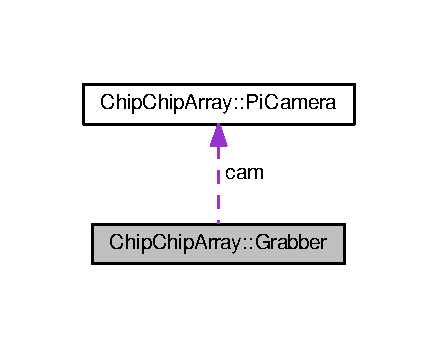
\includegraphics[width=210pt]{classChipChipArray_1_1Grabber__coll__graph}
\end{center}
\end{figure}
\subsection*{Public Member Functions}
\begin{DoxyCompactItemize}
\item 
\hyperlink{classChipChipArray_1_1Grabber_a7333f40c135fbe92d59651f75032b4e7}{Grabber} (\hyperlink{definitions_8hpp_adbd1e7a33d3e1751c7b2aa2562d0ecb9}{Zone} \hyperlink{classChipChipArray_1_1Grabber_ab57efe6e0b6f369b19528285a278d967}{zone}, \hyperlink{definitions_8hpp_a03325a8a9d4f105db5e37dd587128142}{Side} \hyperlink{classChipChipArray_1_1Grabber_a8afbaefae7c767c862fd1bf13968539b}{side})
\item 
void \hyperlink{classChipChipArray_1_1Grabber_aacf089ceb4aa5b263c2cc702fb3daf74}{Close} ()
\item 
\hyperlink{definitions_8hpp_ab84ebabb02540c4a7ec341a213abf1dc}{Result} \hyperlink{classChipChipArray_1_1Grabber_a56639f8f9ba9468bce4b6d69ceb2eb54}{Load} ()
\end{DoxyCompactItemize}
\subsection*{Protected Member Functions}
\begin{DoxyCompactItemize}
\item 
void \hyperlink{classChipChipArray_1_1Grabber_a44e5aeb908634f68de356ad8df3c4bf1}{Deposit} (\hyperlink{definitions_8hpp_abc05a0f46084a3477cf5d5c939ff1436}{Color} color=\hyperlink{definitions_8hpp_abc05a0f46084a3477cf5d5c939ff1436a9594eec95be70e7b1710f730fdda33d9}{Color\+::\+Blue})
\item 
void \hyperlink{classChipChipArray_1_1Grabber_abecb4047b4f7d5a7e691b7fb581b5a39}{Extend} ()
\item 
\hyperlink{classChipChipArray_1_1Block}{Block} \hyperlink{classChipChipArray_1_1Grabber_af49248c957a1695dcde79c0f5f8df99b}{Locate\+Blocks} (\hyperlink{definitions_8hpp_abc05a0f46084a3477cf5d5c939ff1436}{Color} color=\hyperlink{definitions_8hpp_abc05a0f46084a3477cf5d5c939ff1436a1e700ac224a6d34c5b171bb6f462aa41}{Color\+::\+Perrywinkle})
\item 
\hyperlink{classChipChipArray_1_1Block}{Block} \hyperlink{classChipChipArray_1_1Grabber_ab9b0d6a64b2c94c0d0f810a5ebeef6ec}{Locate\+Blue\+Block} ()
\end{DoxyCompactItemize}
\subsection*{Protected Attributes}
\begin{DoxyCompactItemize}
\item 
\hyperlink{classChipChipArray_1_1PiCamera}{Pi\+Camera} \hyperlink{classChipChipArray_1_1Grabber_a726bcc2367a719cb84de92a981947622}{cam}
\item 
\hyperlink{definitions_8hpp_a03325a8a9d4f105db5e37dd587128142}{Side} \hyperlink{classChipChipArray_1_1Grabber_a8afbaefae7c767c862fd1bf13968539b}{side}
\item 
\hyperlink{definitions_8hpp_adbd1e7a33d3e1751c7b2aa2562d0ecb9}{Zone} \hyperlink{classChipChipArray_1_1Grabber_ab57efe6e0b6f369b19528285a278d967}{zone}
\end{DoxyCompactItemize}


\subsection{Detailed Description}
This class finds blocks, identifies them, and sorts them according to color, size, and zone. 

Definition at line \hyperlink{Grabber_8hpp_source_l00030}{30} of file \hyperlink{Grabber_8hpp_source}{Grabber.\+hpp}.



\subsection{Constructor \& Destructor Documentation}
\hypertarget{classChipChipArray_1_1Grabber_a7333f40c135fbe92d59651f75032b4e7}{\index{Chip\+Chip\+Array\+::\+Grabber@{Chip\+Chip\+Array\+::\+Grabber}!Grabber@{Grabber}}
\index{Grabber@{Grabber}!Chip\+Chip\+Array\+::\+Grabber@{Chip\+Chip\+Array\+::\+Grabber}}
\subsubsection[{Grabber}]{\setlength{\rightskip}{0pt plus 5cm}Chip\+Chip\+Array\+::\+Grabber\+::\+Grabber (
\begin{DoxyParamCaption}
\item[{{\bf Zone}}]{zone, }
\item[{{\bf Side}}]{side}
\end{DoxyParamCaption}
)}}\label{classChipChipArray_1_1Grabber_a7333f40c135fbe92d59651f75032b4e7}
Initializes the class according to the side and zone and extends the robotic arm into position.


\begin{DoxyParams}{Parameters}
{\em zone} & the zone (A, B, or C) for which to pick up blocks.\\
\hline
{\em side} & the side from which the robot is moving and the position of the blocks (right or left) in the view of the camera to pick up first \\
\hline
\end{DoxyParams}


Definition at line \hyperlink{Grabber_8hpp_source_l00143}{143} of file \hyperlink{Grabber_8hpp_source}{Grabber.\+hpp}.


\begin{DoxyCode}
00143                                          \{
00144         log.\hyperlink{classChipChipArray_1_1Log_a66575b6e94c6112e4cefa5736cb996e0}{Status}(\textcolor{stringliteral}{"Opening Grabber"});
00145         log.\hyperlink{classChipChipArray_1_1Log_a154a5f38d9c7a767693b242684a3d4d9}{Verbose}(\textcolor{stringliteral}{"Zone: "} + \hyperlink{namespacestd_aa5ddf582a1c96ffe258c997be9a294a3}{std::to\_string}(\hyperlink{classChipChipArray_1_1Grabber_ab57efe6e0b6f369b19528285a278d967}{zone}));
00146         log.\hyperlink{classChipChipArray_1_1Log_a154a5f38d9c7a767693b242684a3d4d9}{Verbose}(\textcolor{stringliteral}{"Side: "} + \hyperlink{namespacestd_aa5ddf582a1c96ffe258c997be9a294a3}{std::to\_string}(\hyperlink{classChipChipArray_1_1Grabber_a8afbaefae7c767c862fd1bf13968539b}{side}));
00147 
00148         this->\hyperlink{classChipChipArray_1_1Grabber_ab57efe6e0b6f369b19528285a278d967}{zone} = \hyperlink{classChipChipArray_1_1Grabber_ab57efe6e0b6f369b19528285a278d967}{zone};
00149         this->\hyperlink{classChipChipArray_1_1Grabber_a8afbaefae7c767c862fd1bf13968539b}{side} = \hyperlink{classChipChipArray_1_1Grabber_a8afbaefae7c767c862fd1bf13968539b}{side};
00150 
00151         log.\hyperlink{classChipChipArray_1_1Log_a154a5f38d9c7a767693b242684a3d4d9}{Verbose}(\textcolor{stringliteral}{"Setting HSV threshold values"});
00152 
00153         rangeVals[\hyperlink{definitions_8hpp_abc05a0f46084a3477cf5d5c939ff1436aee38e4d5dd68c4e440825018d549cb47}{Color::Red}] = \{ cv::Scalar(0, 20, 60),
00154             cv::Scalar(12, 255, 255) \};
00155         rangeVals[\hyperlink{definitions_8hpp_abc05a0f46084a3477cf5d5c939ff1436ad382816a3cbeed082c9e216e7392eed1}{Color::Green}] = \{ cv::Scalar(49, 41, 17),
00156             cv::Scalar(63, 255, 255) \};
00157         rangeVals[\hyperlink{definitions_8hpp_abc05a0f46084a3477cf5d5c939ff1436a9594eec95be70e7b1710f730fdda33d9}{Color::Blue}] = \{ cv::Scalar(70, 0, 0),
00158             cv::Scalar(100, 255, 255) \};
00159 
00160         \textcolor{comment}{/* Remember, we're only pretending this color's image is in HSV space.}
00161 \textcolor{comment}{         * It's really in YUV, as required by Jacob yellow-detection algorithm. */}
00162         rangeVals[\hyperlink{definitions_8hpp_abc05a0f46084a3477cf5d5c939ff1436a51e6cd92b6c45f9affdc158ecca2b8b8}{Color::Yellow}] = \{ cv::Scalar(0, 0, 0),
00163             cv::Scalar(255, 255, 20)\};
00164     \}
\end{DoxyCode}


Here is the call graph for this function\+:
\nopagebreak
\begin{figure}[H]
\begin{center}
\leavevmode
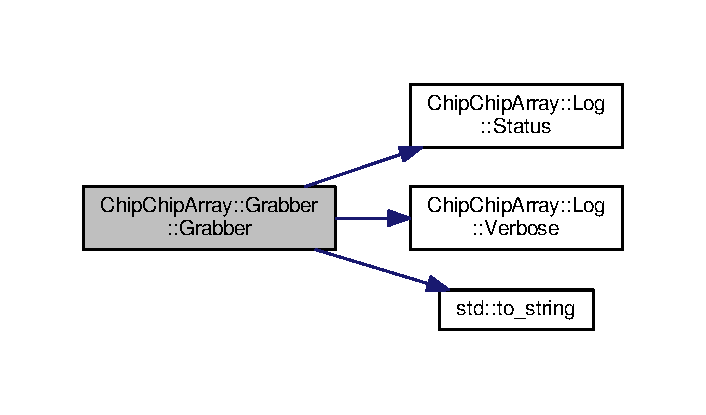
\includegraphics[width=339pt]{classChipChipArray_1_1Grabber_a7333f40c135fbe92d59651f75032b4e7_cgraph}
\end{center}
\end{figure}




\subsection{Member Function Documentation}
\hypertarget{classChipChipArray_1_1Grabber_aacf089ceb4aa5b263c2cc702fb3daf74}{\index{Chip\+Chip\+Array\+::\+Grabber@{Chip\+Chip\+Array\+::\+Grabber}!Close@{Close}}
\index{Close@{Close}!Chip\+Chip\+Array\+::\+Grabber@{Chip\+Chip\+Array\+::\+Grabber}}
\subsubsection[{Close}]{\setlength{\rightskip}{0pt plus 5cm}void Chip\+Chip\+Array\+::\+Grabber\+::\+Close (
\begin{DoxyParamCaption}
{}
\end{DoxyParamCaption}
)}}\label{classChipChipArray_1_1Grabber_aacf089ceb4aa5b263c2cc702fb3daf74}
Closes the \hyperlink{classChipChipArray_1_1Grabber}{Grabber}. Retracts the arm and closes the camera. 

Definition at line \hyperlink{Grabber_8hpp_source_l00166}{166} of file \hyperlink{Grabber_8hpp_source}{Grabber.\+hpp}.


\begin{DoxyCode}
00166                         \{
00167         log.\hyperlink{classChipChipArray_1_1Log_a66575b6e94c6112e4cefa5736cb996e0}{Status}(\textcolor{stringliteral}{"Closing Grabber"});
00168         \hyperlink{classChipChipArray_1_1Grabber_a726bcc2367a719cb84de92a981947622}{cam}.\hyperlink{classChipChipArray_1_1PiCamera_a38f8205921d6deec5a2c360ea7d24cc5}{Close}();
00169     \}
\end{DoxyCode}


Here is the call graph for this function\+:
\nopagebreak
\begin{figure}[H]
\begin{center}
\leavevmode
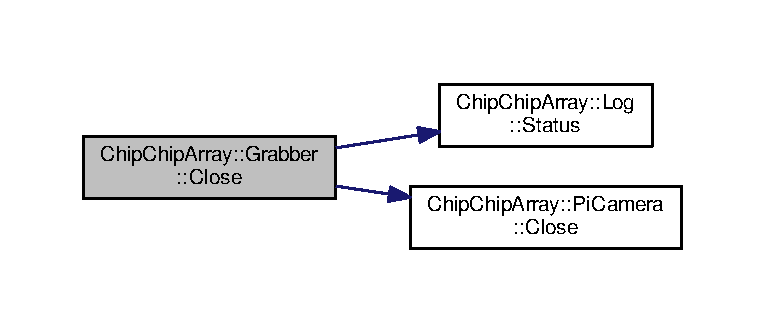
\includegraphics[width=350pt]{classChipChipArray_1_1Grabber_aacf089ceb4aa5b263c2cc702fb3daf74_cgraph}
\end{center}
\end{figure}




Here is the caller graph for this function\+:
\nopagebreak
\begin{figure}[H]
\begin{center}
\leavevmode
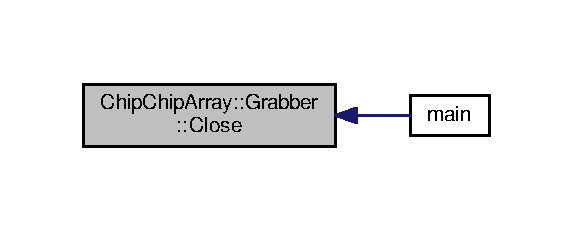
\includegraphics[width=275pt]{classChipChipArray_1_1Grabber_aacf089ceb4aa5b263c2cc702fb3daf74_icgraph}
\end{center}
\end{figure}


\hypertarget{classChipChipArray_1_1Grabber_a44e5aeb908634f68de356ad8df3c4bf1}{\index{Chip\+Chip\+Array\+::\+Grabber@{Chip\+Chip\+Array\+::\+Grabber}!Deposit@{Deposit}}
\index{Deposit@{Deposit}!Chip\+Chip\+Array\+::\+Grabber@{Chip\+Chip\+Array\+::\+Grabber}}
\subsubsection[{Deposit}]{\setlength{\rightskip}{0pt plus 5cm}void Chip\+Chip\+Array\+::\+Grabber\+::\+Deposit (
\begin{DoxyParamCaption}
\item[{{\bf Color}}]{color = {\ttfamily {\bf Color\+::\+Blue}}}
\end{DoxyParamCaption}
)\hspace{0.3cm}{\ttfamily [protected]}}}\label{classChipChipArray_1_1Grabber_a44e5aeb908634f68de356ad8df3c4bf1}
Deposits blocks in the storage/unloading unit. 

Definition at line \hyperlink{Grabber_8hpp_source_l00171}{171} of file \hyperlink{Grabber_8hpp_source}{Grabber.\+hpp}.


\begin{DoxyCode}
00171                                      \{
00172         \textcolor{keywordflow}{if}(color == \hyperlink{definitions_8hpp_abc05a0f46084a3477cf5d5c939ff1436a9594eec95be70e7b1710f730fdda33d9}{Color::Blue}) \{
00173             arm.\hyperlink{classChipChipArray_1_1Arm_a20c6fe3fe79c16f492a8c18b91427080}{ClawClose}();
00174             sleep(1);
00175             arm.\hyperlink{classChipChipArray_1_1Arm_a8b077a3791d9fc5ef285c1520fe4c5d8}{BaseTilt}(160);
00176             sleep(1);
00177             arm.\hyperlink{classChipChipArray_1_1Arm_ac45149e03abfac230b75156bb42e8417}{Elbow}(130);
00178             sleep(1);
00179             arm.\hyperlink{classChipChipArray_1_1Arm_addaedfe85ff2b14ff00c344fc4b40cd6}{BaseTurn}(47);
00180             sleep(1);
00181             arm.\hyperlink{classChipChipArray_1_1Arm_abb33b5bb11034554d632f8c9b95b2c44}{ClawOpen}();
00182             sleep(1);
00183         \} \textcolor{keywordflow}{else} \{
00184             \textcolor{keywordflow}{throw} std::runtime\_error(\textcolor{stringliteral}{"Du Idiot! Die Armbewegungen für diese "}
00185                     \textcolor{stringliteral}{"Farbe sind noch nicht implementiert. Vielleicht sollst "}
00186                     \textcolor{stringliteral}{"du die englische Phrase lernen 'Would you like fries "}
00187                     \textcolor{stringliteral}{"with that?"});
00188         \}
00189     \}
\end{DoxyCode}


Here is the call graph for this function\+:
\nopagebreak
\begin{figure}[H]
\begin{center}
\leavevmode
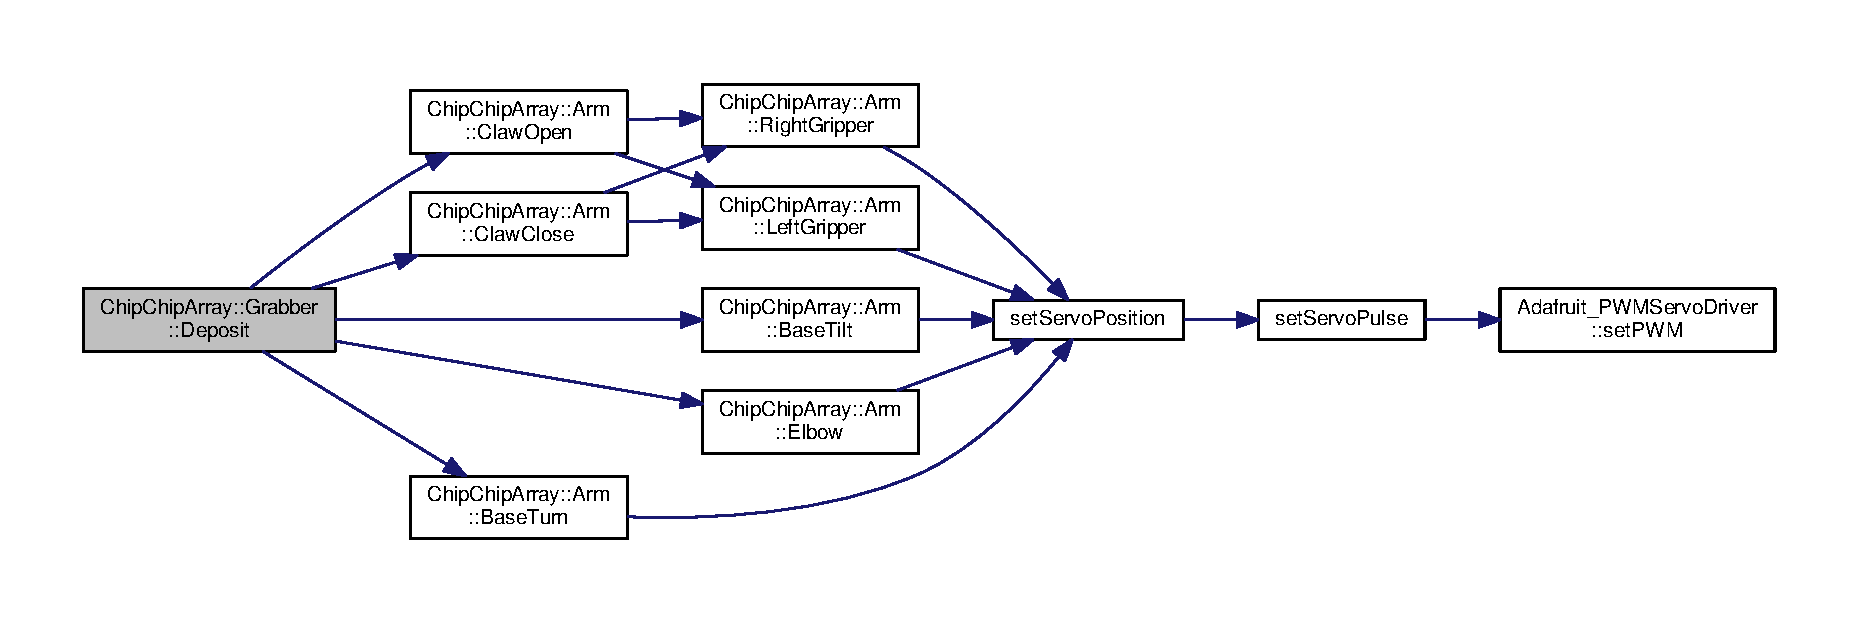
\includegraphics[width=350pt]{classChipChipArray_1_1Grabber_a44e5aeb908634f68de356ad8df3c4bf1_cgraph}
\end{center}
\end{figure}




Here is the caller graph for this function\+:
\nopagebreak
\begin{figure}[H]
\begin{center}
\leavevmode
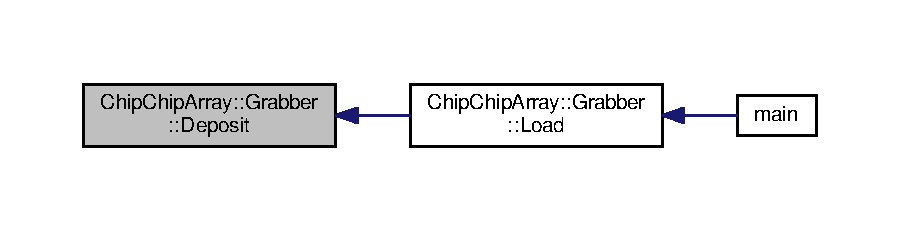
\includegraphics[width=350pt]{classChipChipArray_1_1Grabber_a44e5aeb908634f68de356ad8df3c4bf1_icgraph}
\end{center}
\end{figure}


\hypertarget{classChipChipArray_1_1Grabber_abecb4047b4f7d5a7e691b7fb581b5a39}{\index{Chip\+Chip\+Array\+::\+Grabber@{Chip\+Chip\+Array\+::\+Grabber}!Extend@{Extend}}
\index{Extend@{Extend}!Chip\+Chip\+Array\+::\+Grabber@{Chip\+Chip\+Array\+::\+Grabber}}
\subsubsection[{Extend}]{\setlength{\rightskip}{0pt plus 5cm}void Chip\+Chip\+Array\+::\+Grabber\+::\+Extend (
\begin{DoxyParamCaption}
{}
\end{DoxyParamCaption}
)\hspace{0.3cm}{\ttfamily [protected]}}}\label{classChipChipArray_1_1Grabber_abecb4047b4f7d5a7e691b7fb581b5a39}
Sets arm to generic position roughly right above a stack of blocks. 

Definition at line \hyperlink{Grabber_8hpp_source_l00191}{191} of file \hyperlink{Grabber_8hpp_source}{Grabber.\+hpp}.


\begin{DoxyCode}
00191                          \{
00192         arm.\hyperlink{classChipChipArray_1_1Arm_ac45149e03abfac230b75156bb42e8417}{Elbow}(180);
00193         usleep(500000);
00194         arm.\hyperlink{classChipChipArray_1_1Arm_addaedfe85ff2b14ff00c344fc4b40cd6}{BaseTurn}(132);
00195         arm.\hyperlink{classChipChipArray_1_1Arm_a8b077a3791d9fc5ef285c1520fe4c5d8}{BaseTilt}(125);
00196         arm.\hyperlink{classChipChipArray_1_1Arm_ac45149e03abfac230b75156bb42e8417}{Elbow}(150);
00197         arm.\hyperlink{classChipChipArray_1_1Arm_a35ec7756840d9d32dcfbb88d831f087f}{WristTwist}(90);
00198         arm.\hyperlink{classChipChipArray_1_1Arm_abb33b5bb11034554d632f8c9b95b2c44}{ClawOpen}();
00199         sleep(2);
00200     \}
\end{DoxyCode}


Here is the call graph for this function\+:
\nopagebreak
\begin{figure}[H]
\begin{center}
\leavevmode
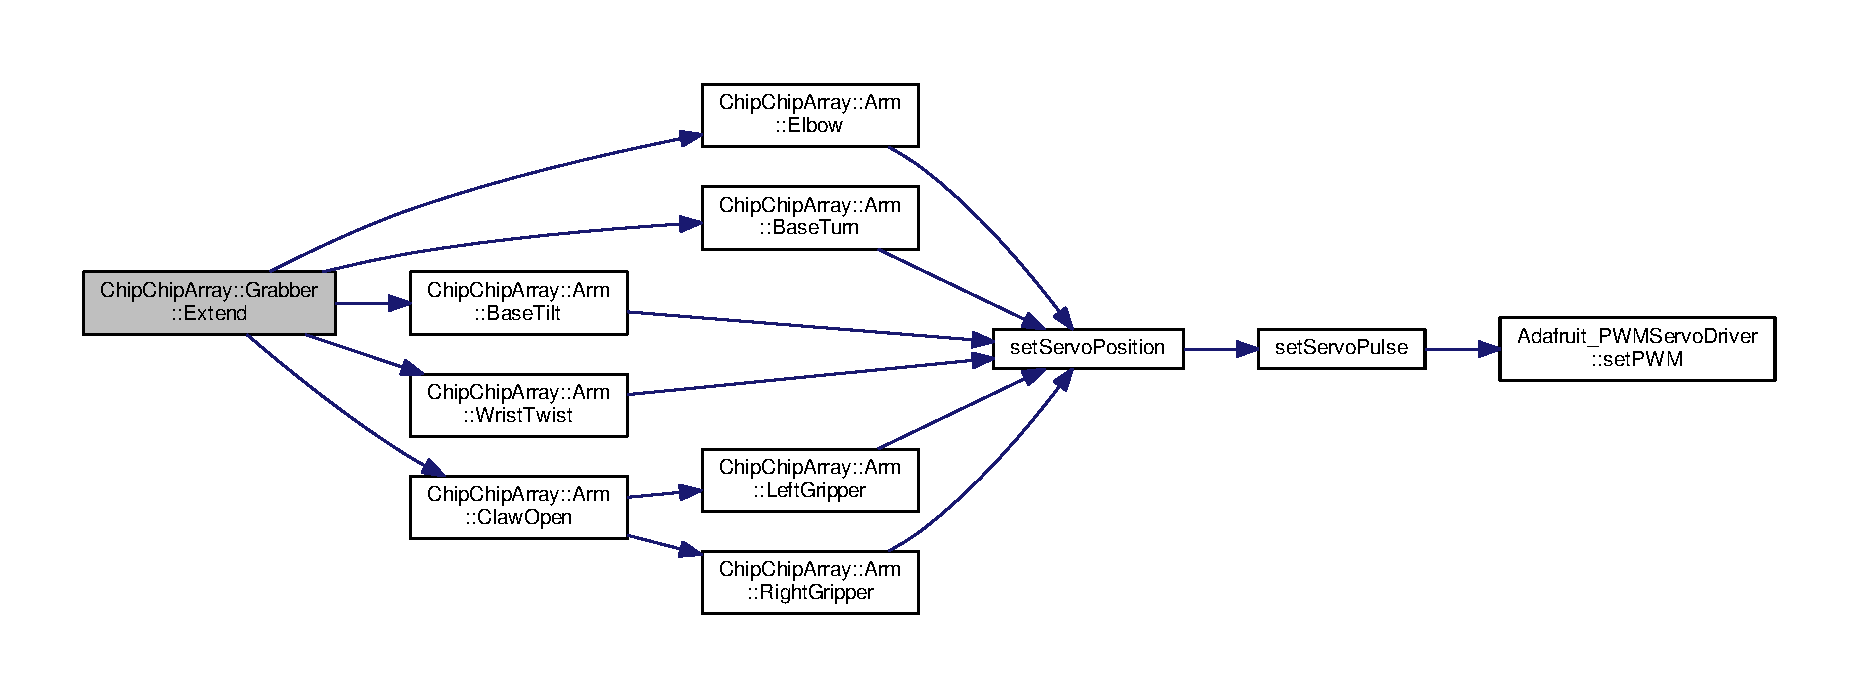
\includegraphics[width=350pt]{classChipChipArray_1_1Grabber_abecb4047b4f7d5a7e691b7fb581b5a39_cgraph}
\end{center}
\end{figure}




Here is the caller graph for this function\+:
\nopagebreak
\begin{figure}[H]
\begin{center}
\leavevmode
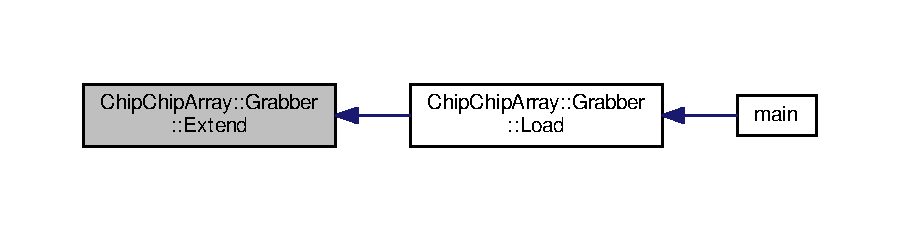
\includegraphics[width=350pt]{classChipChipArray_1_1Grabber_abecb4047b4f7d5a7e691b7fb581b5a39_icgraph}
\end{center}
\end{figure}


\hypertarget{classChipChipArray_1_1Grabber_a56639f8f9ba9468bce4b6d69ceb2eb54}{\index{Chip\+Chip\+Array\+::\+Grabber@{Chip\+Chip\+Array\+::\+Grabber}!Load@{Load}}
\index{Load@{Load}!Chip\+Chip\+Array\+::\+Grabber@{Chip\+Chip\+Array\+::\+Grabber}}
\subsubsection[{Load}]{\setlength{\rightskip}{0pt plus 5cm}{\bf Result} Chip\+Chip\+Array\+::\+Grabber\+::\+Load (
\begin{DoxyParamCaption}
{}
\end{DoxyParamCaption}
)}}\label{classChipChipArray_1_1Grabber_a56639f8f9ba9468bce4b6d69ceb2eb54}
Loads a block(s) (if possible) at the robot's current position.

\begin{DoxyReturn}{Returns}
the number of half and whole blocks loaded 
\end{DoxyReturn}


Definition at line \hyperlink{Grabber_8hpp_source_l00202}{202} of file \hyperlink{Grabber_8hpp_source}{Grabber.\+hpp}.


\begin{DoxyCode}
00202                          \{
00203         \textcolor{keywordflow}{for}(\hyperlink{definitions_8hpp_adde6aaee8457bee49c2a92621fe22b79}{uint8} i = 0; i < 2; i++) \{
00204             \hyperlink{classChipChipArray_1_1Grabber_abecb4047b4f7d5a7e691b7fb581b5a39}{Extend}();
00205 
00206             \textcolor{keywordflow}{try} \{
00207                 Block block = (\hyperlink{classChipChipArray_1_1Grabber_ab57efe6e0b6f369b19528285a278d967}{zone} == \hyperlink{definitions_8hpp_adbd1e7a33d3e1751c7b2aa2562d0ecb9a7fc56270e7a70fa81a5935b72eacbe29}{Zone::A})
00208                     ? \hyperlink{classChipChipArray_1_1Grabber_af49248c957a1695dcde79c0f5f8df99b}{LocateBlocks}(\hyperlink{definitions_8hpp_abc05a0f46084a3477cf5d5c939ff1436a9594eec95be70e7b1710f730fdda33d9}{Color::Blue}) : 
      \hyperlink{classChipChipArray_1_1Grabber_ab9b0d6a64b2c94c0d0f810a5ebeef6ec}{LocateBlueBlock}();
00209 
00210                 \hyperlink{definitions_8hpp_aacdc525d6f7bddb3ae95d5c311bd06a1}{float32} baseKonstant = 0.5;
00211                 \textcolor{keywordflow}{if}(block.dRightLeft > 0) baseKonstant *= -1;
00212                 \hyperlink{definitions_8hpp_aacdc525d6f7bddb3ae95d5c311bd06a1}{float32} degree = baseKonstant * std::sqrt(block.dRightLeft);
00213                 arm.\hyperlink{classChipChipArray_1_1Arm_a980f5bd278cbe06aa21754fb8e0324b3}{dBaseTurn}(degree);
00214                 arm.\hyperlink{classChipChipArray_1_1Arm_a6bde822b1be63926e21222f36aad67b3}{dWristTwist}(-degree);
00215                 sleep(1);
00216                 arm.\hyperlink{classChipChipArray_1_1Arm_a8b077a3791d9fc5ef285c1520fe4c5d8}{BaseTilt}(140);
00217                 sleep(1);
00218 
00219                 \hyperlink{definitions_8hpp_adde6aaee8457bee49c2a92621fe22b79}{uint8} bend = (i == 0 ? 100 : 90);
00220 
00221                 \textcolor{comment}{// lower claw over block}
00222                 \textcolor{keywordflow}{for}(\hyperlink{definitions_8hpp_adde6aaee8457bee49c2a92621fe22b79}{uint8} j = 140; j >= bend; j -= 10) \{
00223                     arm.\hyperlink{classChipChipArray_1_1Arm_ac45149e03abfac230b75156bb42e8417}{Elbow}(j);
00224                     sleep(1);
00225                 \}
00226 
00227                 \textcolor{comment}{// deposit in bin}
00228                 sleep(1);
00229                 \hyperlink{classChipChipArray_1_1Grabber_a44e5aeb908634f68de356ad8df3c4bf1}{Deposit}();
00230             \} \textcolor{keywordflow}{catch}(std::exception ex) \{
00231                 log.\hyperlink{classChipChipArray_1_1Log_aba7b7b0555f49f4dcf15f4b9fd3e6b34}{Error}(std::string(\textcolor{stringliteral}{"An exception occured attempting "}
00232                             \textcolor{stringliteral}{"to load the blocks in function Grabber::Load(): "}) 
00233                         + ex.what());
00234             \}
00235 
00236 
00237             \textcolor{keywordflow}{if}(i == 0) \{
00238                 arm.\hyperlink{classChipChipArray_1_1Arm_addaedfe85ff2b14ff00c344fc4b40cd6}{BaseTurn}(132);
00239             \} \textcolor{keywordflow}{else} \{
00240                 arm.\hyperlink{classChipChipArray_1_1Arm_addaedfe85ff2b14ff00c344fc4b40cd6}{BaseTurn}(135);
00241                 sleep(1);
00242                 arm.\hyperlink{classChipChipArray_1_1Arm_a8b077a3791d9fc5ef285c1520fe4c5d8}{BaseTilt}(180);
00243                 sleep(1);
00244                 arm.\hyperlink{classChipChipArray_1_1Arm_ac45149e03abfac230b75156bb42e8417}{Elbow}(90);
00245                 sleep(1);
00246                 arm.\hyperlink{classChipChipArray_1_1Arm_ac45149e03abfac230b75156bb42e8417}{Elbow}(45);
00247                 sleep(1);
00248                 arm.\hyperlink{classChipChipArray_1_1Arm_ac45149e03abfac230b75156bb42e8417}{Elbow}(0);
00249             \}
00250         \}
00251     \}
\end{DoxyCode}


Here is the call graph for this function\+:
\nopagebreak
\begin{figure}[H]
\begin{center}
\leavevmode
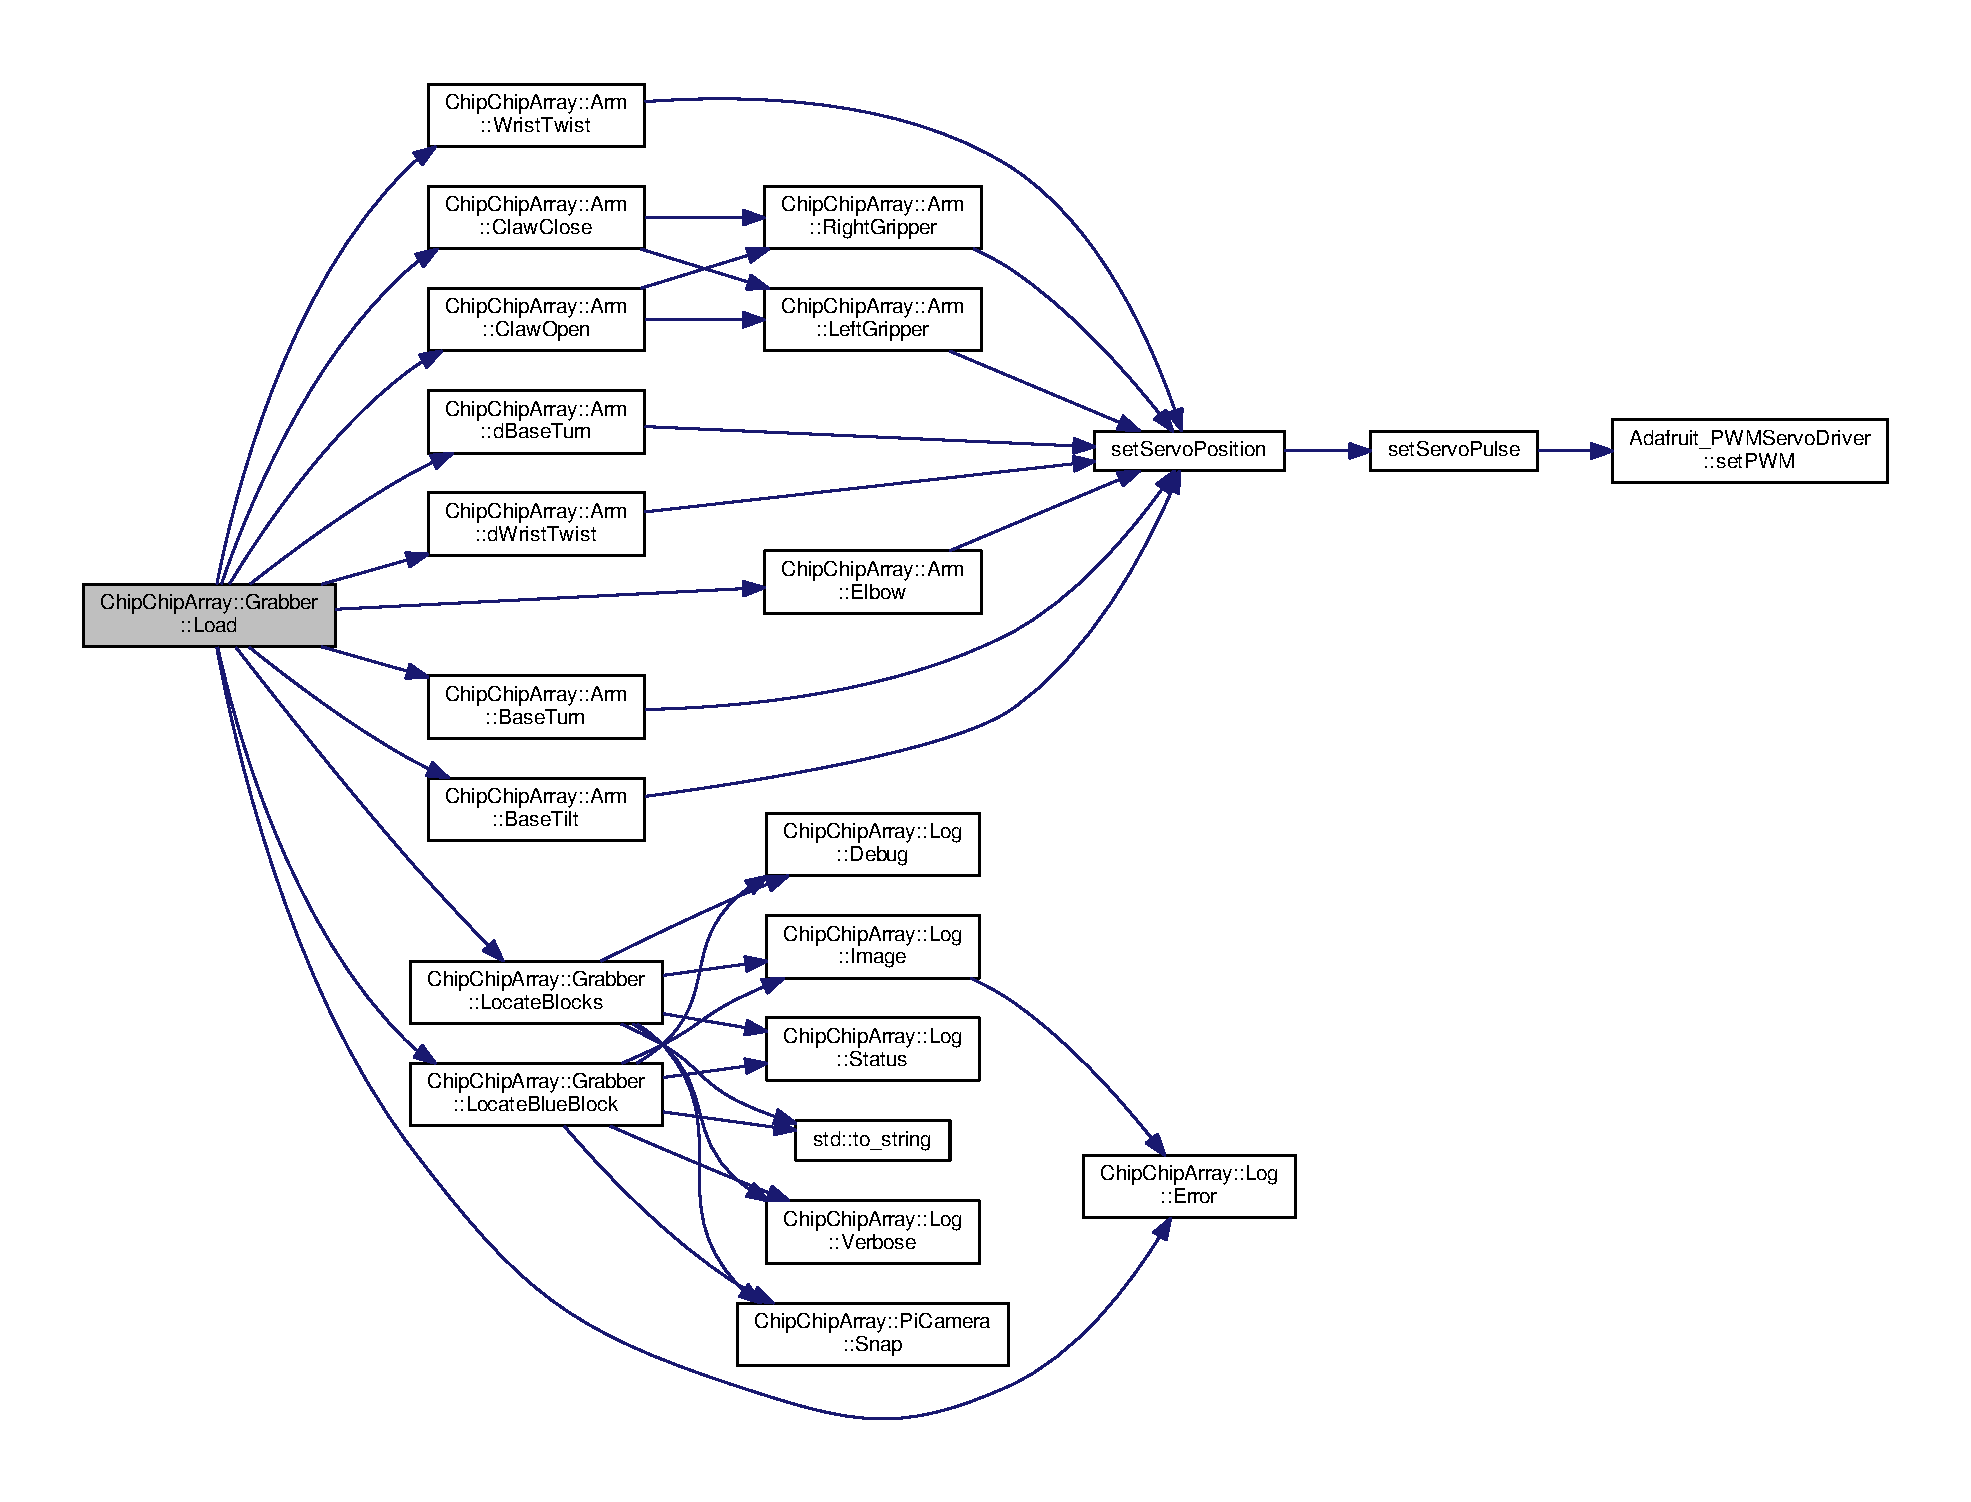
\includegraphics[width=350pt]{classChipChipArray_1_1Grabber_a56639f8f9ba9468bce4b6d69ceb2eb54_cgraph}
\end{center}
\end{figure}




Here is the caller graph for this function\+:
\nopagebreak
\begin{figure}[H]
\begin{center}
\leavevmode
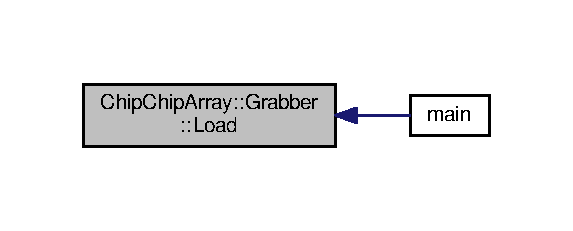
\includegraphics[width=275pt]{classChipChipArray_1_1Grabber_a56639f8f9ba9468bce4b6d69ceb2eb54_icgraph}
\end{center}
\end{figure}


\hypertarget{classChipChipArray_1_1Grabber_af49248c957a1695dcde79c0f5f8df99b}{\index{Chip\+Chip\+Array\+::\+Grabber@{Chip\+Chip\+Array\+::\+Grabber}!Locate\+Blocks@{Locate\+Blocks}}
\index{Locate\+Blocks@{Locate\+Blocks}!Chip\+Chip\+Array\+::\+Grabber@{Chip\+Chip\+Array\+::\+Grabber}}
\subsubsection[{Locate\+Blocks}]{\setlength{\rightskip}{0pt plus 5cm}{\bf Block} Chip\+Chip\+Array\+::\+Grabber\+::\+Locate\+Blocks (
\begin{DoxyParamCaption}
\item[{{\bf Color}}]{color = {\ttfamily {\bf Color\+::\+Perrywinkle}}}
\end{DoxyParamCaption}
)\hspace{0.3cm}{\ttfamily [protected]}}}\label{classChipChipArray_1_1Grabber_af49248c957a1695dcde79c0f5f8df99b}
Loads a stack of blocks for all zones. Does multiple colors and both sizes.


\begin{DoxyParams}{Parameters}
{\em color} & the color block for which to search. Perrywinkle denotes searching for all colors (because who actually knows what color perrywinkle is?).\\
\hline
\end{DoxyParams}
\begin{DoxyReturn}{Returns}
\hyperlink{classChipChipArray_1_1Block}{Block} instance representing the block found 
\end{DoxyReturn}


Definition at line \hyperlink{Grabber_8hpp_source_l00254}{254} of file \hyperlink{Grabber_8hpp_source}{Grabber.\+hpp}.


\begin{DoxyCode}
00254                                            \{
00255         invokeCount++;
00256         std::string logstr = \textcolor{stringliteral}{"Locating blocks"};
00257 
00258         \textcolor{keywordflow}{if}(color == \hyperlink{definitions_8hpp_abc05a0f46084a3477cf5d5c939ff1436a1e700ac224a6d34c5b171bb6f462aa41}{Color::Perrywinkle}) \{
00259             logstr += \textcolor{stringliteral}{" ("} + \hyperlink{namespacestd_aa5ddf582a1c96ffe258c997be9a294a3}{std::to\_string}(color) + \textcolor{stringliteral}{")"};
00260         \}
00261 
00262         log.\hyperlink{classChipChipArray_1_1Log_a154a5f38d9c7a767693b242684a3d4d9}{Verbose}(logstr);
00263 
00264         cv::Mat imgOrig;
00265         cv::transpose(\hyperlink{classChipChipArray_1_1Grabber_a726bcc2367a719cb84de92a981947622}{cam}.\hyperlink{classChipChipArray_1_1PiCamera_a58fb0de02570dce9a9cb60a1a04fb84f}{Snap}(), imgOrig);
00266 
00267         cv::Mat imgHSV;
00268         cv::Mat imgThresh;
00269         std::vector<cv::Rect> blocks;
00270         std::vector<Color> colors;
00271 
00272         \hyperlink{definitions_8hpp_adde6aaee8457bee49c2a92621fe22b79}{uint8} loopNum = (color == \hyperlink{definitions_8hpp_abc05a0f46084a3477cf5d5c939ff1436a1e700ac224a6d34c5b171bb6f462aa41}{Color::Perrywinkle} ? rangeVals.size() : 1);
00273 
00274         \textcolor{keywordflow}{for}(\textcolor{keywordtype}{int} i = 0; i < loopNum; i++) \{
00275             \textcolor{keywordflow}{if}(loopNum > 1) \{
00276                 \textcolor{keywordflow}{switch}(i) \{
00277                     \textcolor{keywordflow}{case} 0:
00278                         color = \hyperlink{definitions_8hpp_abc05a0f46084a3477cf5d5c939ff1436aee38e4d5dd68c4e440825018d549cb47}{Color::Red};
00279                         \textcolor{keywordflow}{break};
00280 
00281                     \textcolor{keywordflow}{case} 1:
00282                         color = \hyperlink{definitions_8hpp_abc05a0f46084a3477cf5d5c939ff1436ad382816a3cbeed082c9e216e7392eed1}{Color::Green};
00283                         \textcolor{keywordflow}{break};
00284 
00285                     \textcolor{keywordflow}{case} 2:
00286                         color = \hyperlink{definitions_8hpp_abc05a0f46084a3477cf5d5c939ff1436a9594eec95be70e7b1710f730fdda33d9}{Color::Blue};
00287                         \textcolor{keywordflow}{break};
00288 
00289                         \textcolor{comment}{/* Must be last, because it changes imgHSV from HSV space}
00290 \textcolor{comment}{                         * to YUV space. */}
00291                     \textcolor{keywordflow}{case} 3: 
00292                         color = \hyperlink{definitions_8hpp_abc05a0f46084a3477cf5d5c939ff1436a51e6cd92b6c45f9affdc158ecca2b8b8}{Color::Yellow};
00293                         \textcolor{keywordflow}{break};
00294                 \}
00295             \}
00296 
00297             log.\hyperlink{classChipChipArray_1_1Log_a154a5f38d9c7a767693b242684a3d4d9}{Verbose}(\textcolor{stringliteral}{"Searching: "} + \hyperlink{namespacestd_aa5ddf582a1c96ffe258c997be9a294a3}{std::to\_string}(color));
00298 
00299             \textcolor{keywordflow}{if}(color == \hyperlink{definitions_8hpp_abc05a0f46084a3477cf5d5c939ff1436a51e6cd92b6c45f9affdc158ecca2b8b8}{Color::Yellow}) \{
00300                 cv::Mat temp;
00301                 imgOrig.copyTo(temp);
00302                 cv::cvtColor(imgOrig, imgHSV, CV\_BGR2YUV);
00303                 cv::cvtColor(imgHSV, temp, CV\_HSV2BGR);
00304                 cv::cvtColor(temp, imgHSV, cv::COLOR\_BGR2HSV);
00305                 log.\hyperlink{classChipChipArray_1_1Log_a65bbab057c8b1453f9e4efcfee7522c4}{Image}(temp, \textcolor{stringliteral}{"yuv\_yellow\_"} + \hyperlink{namespacestd_aa5ddf582a1c96ffe258c997be9a294a3}{std::to\_string}(color)
00306                         + \textcolor{stringliteral}{"\_"} + \hyperlink{namespacestd_aa5ddf582a1c96ffe258c997be9a294a3}{std::to\_string}(\hyperlink{classChipChipArray_1_1Grabber_ab57efe6e0b6f369b19528285a278d967}{zone})
00307                         + \hyperlink{namespacestd_aa5ddf582a1c96ffe258c997be9a294a3}{std::to\_string}(invokeCount)
00308                         + \textcolor{stringliteral}{".bmp"});
00309             \} \textcolor{keywordflow}{else} \{
00310                 cv::cvtColor(imgOrig, imgHSV, cv::COLOR\_BGR2HSV);
00311             \}
00312 
00313             cv::inRange(imgHSV, rangeVals[color][0],
00314                     rangeVals[color][1], imgThresh);
00315 
00316             \textcolor{comment}{/* }
00317 \textcolor{comment}{             * Not quite sure what all this does, but it seems to}
00318 \textcolor{comment}{             * relate to smoothing the image}
00319 \textcolor{comment}{             */}
00320             cv::erode(imgThresh, imgThresh,
00321                     cv::getStructuringElement(
00322                         cv::MORPH\_ELLIPSE,
00323                         \hyperlink{definitions_8hpp_a9809446fd16a744b6df9808293f14153}{cv::Size}(5, 5)));
00324             cv::dilate(imgThresh, imgThresh,
00325                     cv::getStructuringElement(
00326                         cv::MORPH\_ELLIPSE,
00327                         \hyperlink{definitions_8hpp_a9809446fd16a744b6df9808293f14153}{cv::Size}(5, 5)));
00328             cv::dilate(imgThresh, imgThresh,
00329                     cv::getStructuringElement(
00330                         cv::MORPH\_ELLIPSE,
00331                         \hyperlink{definitions_8hpp_a9809446fd16a744b6df9808293f14153}{cv::Size}(5, 5)));
00332             cv::erode(imgThresh, imgThresh,
00333                     cv::getStructuringElement(
00334                         cv::MORPH\_ELLIPSE,
00335                         \hyperlink{definitions_8hpp_a9809446fd16a744b6df9808293f14153}{cv::Size}(5, 5)));
00336 
00337             log.\hyperlink{classChipChipArray_1_1Log_a65bbab057c8b1453f9e4efcfee7522c4}{Image}(imgThresh, \textcolor{stringliteral}{"thresh\_"} + \hyperlink{namespacestd_aa5ddf582a1c96ffe258c997be9a294a3}{std::to\_string}(color)
00338                     + \textcolor{stringliteral}{"\_"} + \hyperlink{namespacestd_aa5ddf582a1c96ffe258c997be9a294a3}{std::to\_string}(\hyperlink{classChipChipArray_1_1Grabber_ab57efe6e0b6f369b19528285a278d967}{zone})
00339                     + \hyperlink{namespacestd_aa5ddf582a1c96ffe258c997be9a294a3}{std::to\_string}(invokeCount)
00340                     + \textcolor{stringliteral}{".bmp"});
00341 
00342             \textcolor{comment}{// calculate contours}
00343             std::vector<std::vector<cv::Point>> contours;
00344             cv::findContours(imgThresh, contours, CV\_RETR\_TREE,
00345                     CV\_CHAIN\_APPROX\_SIMPLE,
00346                     cv::Point(0, 0));
00347             std::vector<std::vector<cv::Point>>
00348                 contours\_poly(contours.size());
00349             std::vector<cv::Rect> bounds(contours.size());
00350 
00351             \textcolor{comment}{// find rectangle around polygon-ish shapes}
00352             \textcolor{keywordflow}{for}(\textcolor{keywordtype}{int} i = 0; i < contours.size(); i++) \{
00353                 \hyperlink{definitions_8hpp_a1134b580f8da4de94ca6b1de4d37975e}{uint32} area = cv::contourArea(contours[i]);
00354 
00355                 \textcolor{comment}{// determine if block and add to blocks vector}
00356                 \textcolor{keywordflow}{if}(area > MIN\_HALF\_BLOCK\_SIZE) \{
00357                     cv::approxPolyDP(cv::Mat(contours[i]),
00358                             contours\_poly[i], 20,
00359                             \textcolor{keyword}{false});
00360                     cv::Rect rect = cv::boundingRect(
00361                             cv::Mat(contours\_poly[i]));
00362                     log.\hyperlink{classChipChipArray_1_1Log_ac32b435af1577e4ebc67af2bdfea8eff}{Debug}(\hyperlink{namespacestd_aa5ddf582a1c96ffe258c997be9a294a3}{std::to\_string}(color)
00363                             + \textcolor{stringliteral}{" block detected "}
00364                             \textcolor{stringliteral}{"with area "}
00365                             + \hyperlink{namespacestd_aa5ddf582a1c96ffe258c997be9a294a3}{std::to\_string}(
00366                                 area));
00367                     blocks.push\_back(rect);
00368                     colors.push\_back(color);
00369                 \}
00370             \}
00371         \}
00372 
00373         \textcolor{keywordflow}{if}(blocks.size() == 0) \{
00374             log.\hyperlink{classChipChipArray_1_1Log_a65bbab057c8b1453f9e4efcfee7522c4}{Image}(imgOrig, \textcolor{stringliteral}{"original\_"} + \hyperlink{namespacestd_aa5ddf582a1c96ffe258c997be9a294a3}{std::to\_string}(
      \hyperlink{classChipChipArray_1_1Grabber_ab57efe6e0b6f369b19528285a278d967}{zone})
00375                     + \hyperlink{namespacestd_aa5ddf582a1c96ffe258c997be9a294a3}{std::to\_string}(invokeCount)
00376                     + \textcolor{stringliteral}{"\_no\_blocks.bmp"});
00377             \textcolor{keywordflow}{throw} std::runtime\_error(\textcolor{stringliteral}{"No blocks found!"});
00378         \} \textcolor{keywordflow}{else} \{
00379             log.\hyperlink{classChipChipArray_1_1Log_a66575b6e94c6112e4cefa5736cb996e0}{Status}(\hyperlink{namespacestd_aa5ddf582a1c96ffe258c997be9a294a3}{std::to\_string}(blocks.size())
00380                     + \textcolor{stringliteral}{" blocks found"});
00381         \}
00382 
00383         \textcolor{comment}{// coordinates start in top right}
00384         Block block = Block(blocks[0], colors[0]);
00385 
00386         \textcolor{keywordflow}{if}(blocks.size() > 1) \{
00387             \textcolor{keywordflow}{for}(\textcolor{keywordtype}{int} i = 1; i < blocks.size(); i++) \{ 
00388                 \textcolor{keywordflow}{if}((\hyperlink{classChipChipArray_1_1Grabber_a8afbaefae7c767c862fd1bf13968539b}{side} == \hyperlink{definitions_8hpp_a03325a8a9d4f105db5e37dd587128142a92b09c7c48c520c3c55e497875da437c}{Side::Right} && blocks[i].x 
00389                             > block.topLeft.x)
00390                         || (\hyperlink{classChipChipArray_1_1Grabber_a8afbaefae7c767c862fd1bf13968539b}{side} == \hyperlink{definitions_8hpp_a03325a8a9d4f105db5e37dd587128142a945d5e233cf7d6240f6b783b36a374ff}{Side::Left}
00391                             && blocks[i].x
00392                             < block.topLeft.x)) \{
00393                     block = Block(blocks[i], colors[i]);
00394                 \}
00395             \}
00396         \}
00397 
00398         log.\hyperlink{classChipChipArray_1_1Log_a66575b6e94c6112e4cefa5736cb996e0}{Status}(\hyperlink{namespacestd_aa5ddf582a1c96ffe258c997be9a294a3}{std::to\_string}(block.color) + \textcolor{stringliteral}{" block is located"});
00399 
00400         log.\hyperlink{classChipChipArray_1_1Log_ac32b435af1577e4ebc67af2bdfea8eff}{Debug}(\textcolor{stringliteral}{"Block properties => area: "} + \hyperlink{namespacestd_aa5ddf582a1c96ffe258c997be9a294a3}{std::to\_string}(block.area)
00401                 + \textcolor{stringliteral}{", height: "} + \hyperlink{namespacestd_aa5ddf582a1c96ffe258c997be9a294a3}{std::to\_string}(block.height) + \textcolor{stringliteral}{", width: "}
00402                 + \hyperlink{namespacestd_aa5ddf582a1c96ffe258c997be9a294a3}{std::to\_string}(block.width) + \textcolor{stringliteral}{", offset: "}
00403                 + \hyperlink{namespacestd_aa5ddf582a1c96ffe258c997be9a294a3}{std::to\_string}(block.offset) + \textcolor{stringliteral}{", color: "}
00404                 + \hyperlink{namespacestd_aa5ddf582a1c96ffe258c997be9a294a3}{std::to\_string}(block.color) + \textcolor{stringliteral}{", size: "}
00405                 + \hyperlink{namespacestd_aa5ddf582a1c96ffe258c997be9a294a3}{std::to\_string}(block.size));
00406 
00407         \textcolor{comment}{/* }
00408 \textcolor{comment}{         * Draw surrounding rectangles from above on original}
00409 \textcolor{comment}{         * image.}
00410 \textcolor{comment}{         */}
00411         cv::rectangle(imgOrig, block.topLeft , block.bottomRight,
00412                 cv::Scalar(255, 0, 0), 4, 8);
00413         log.\hyperlink{classChipChipArray_1_1Log_a65bbab057c8b1453f9e4efcfee7522c4}{Image}(imgOrig, \textcolor{stringliteral}{"original\_"} + \hyperlink{namespacestd_aa5ddf582a1c96ffe258c997be9a294a3}{std::to\_string}(\hyperlink{classChipChipArray_1_1Grabber_ab57efe6e0b6f369b19528285a278d967}{zone})
00414                 + \hyperlink{namespacestd_aa5ddf582a1c96ffe258c997be9a294a3}{std::to\_string}(invokeCount)
00415                 + \textcolor{stringliteral}{".bmp"});
00416 
00417         \textcolor{keywordflow}{return} block;
00418     \}
\end{DoxyCode}


Here is the call graph for this function\+:
\nopagebreak
\begin{figure}[H]
\begin{center}
\leavevmode
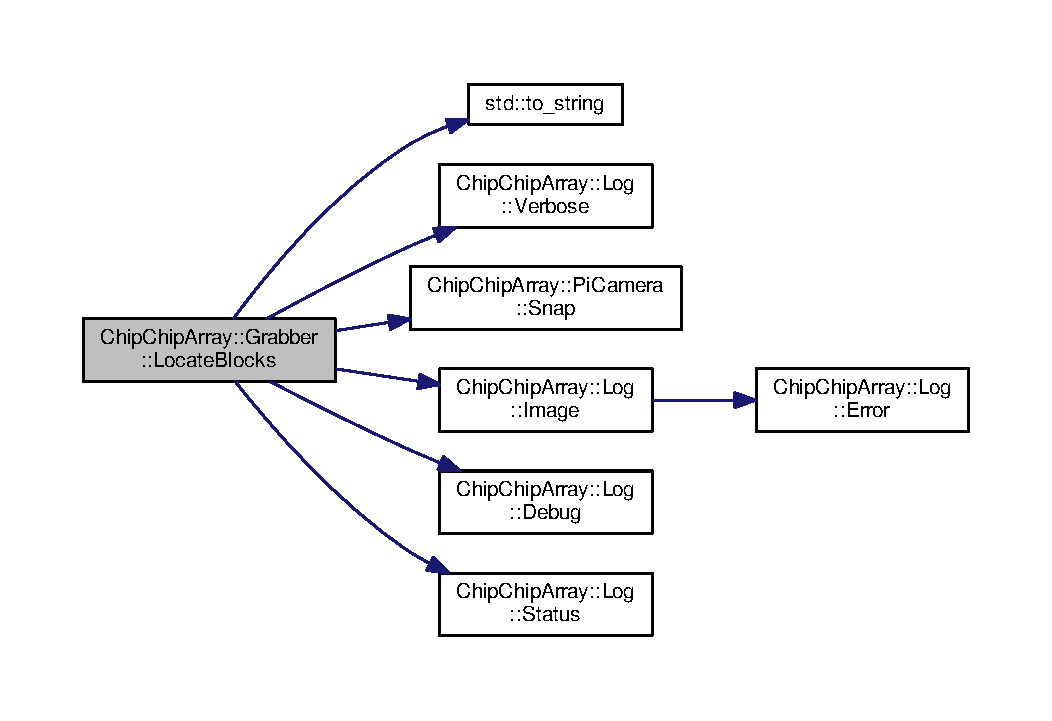
\includegraphics[width=350pt]{classChipChipArray_1_1Grabber_af49248c957a1695dcde79c0f5f8df99b_cgraph}
\end{center}
\end{figure}




Here is the caller graph for this function\+:
\nopagebreak
\begin{figure}[H]
\begin{center}
\leavevmode
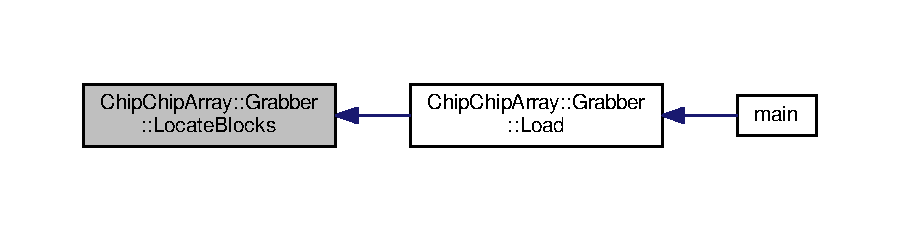
\includegraphics[width=350pt]{classChipChipArray_1_1Grabber_af49248c957a1695dcde79c0f5f8df99b_icgraph}
\end{center}
\end{figure}


\hypertarget{classChipChipArray_1_1Grabber_ab9b0d6a64b2c94c0d0f810a5ebeef6ec}{\index{Chip\+Chip\+Array\+::\+Grabber@{Chip\+Chip\+Array\+::\+Grabber}!Locate\+Blue\+Block@{Locate\+Blue\+Block}}
\index{Locate\+Blue\+Block@{Locate\+Blue\+Block}!Chip\+Chip\+Array\+::\+Grabber@{Chip\+Chip\+Array\+::\+Grabber}}
\subsubsection[{Locate\+Blue\+Block}]{\setlength{\rightskip}{0pt plus 5cm}{\bf Block} Chip\+Chip\+Array\+::\+Grabber\+::\+Locate\+Blue\+Block (
\begin{DoxyParamCaption}
{}
\end{DoxyParamCaption}
)\hspace{0.3cm}{\ttfamily [protected]}}}\label{classChipChipArray_1_1Grabber_ab9b0d6a64b2c94c0d0f810a5ebeef6ec}
Finds whole, blue blocks.

\begin{DoxyReturn}{Returns}
\hyperlink{classChipChipArray_1_1Block}{Block} instance representing the block found 
\end{DoxyReturn}


Definition at line \hyperlink{Grabber_8hpp_source_l00420}{420} of file \hyperlink{Grabber_8hpp_source}{Grabber.\+hpp}.


\begin{DoxyCode}
00420                                    \{
00421         std::vector<cv::Mat> channels;
00422         std::vector<cv::Rect> blocks;   
00423 
00424         invokeCount++;
00425         log.\hyperlink{classChipChipArray_1_1Log_a66575b6e94c6112e4cefa5736cb996e0}{Status}(\textcolor{stringliteral}{"Locating blue blocks"});
00426 
00427         cv::Mat img;
00428         cv::Mat imgThresh;
00429         cv::split(\hyperlink{classChipChipArray_1_1Grabber_a726bcc2367a719cb84de92a981947622}{cam}.\hyperlink{classChipChipArray_1_1PiCamera_a58fb0de02570dce9a9cb60a1a04fb84f}{Snap}(), channels);
00430         cv::transpose(channels[0], img);
00431 
00432         log.\hyperlink{classChipChipArray_1_1Log_a154a5f38d9c7a767693b242684a3d4d9}{Verbose}(\textcolor{stringliteral}{"Searching: Blue block"});
00433         cv::inRange(img, 30, 255, imgThresh);
00434         log.\hyperlink{classChipChipArray_1_1Log_a65bbab057c8b1453f9e4efcfee7522c4}{Image}(imgThresh, \textcolor{stringliteral}{"thresh\_blue"} + \hyperlink{namespacestd_aa5ddf582a1c96ffe258c997be9a294a3}{std::to\_string}(
      \hyperlink{classChipChipArray_1_1Grabber_ab57efe6e0b6f369b19528285a278d967}{zone})
00435                 + \hyperlink{namespacestd_aa5ddf582a1c96ffe258c997be9a294a3}{std::to\_string}(invokeCount) + \textcolor{stringliteral}{".bmp"});
00436 
00437         \textcolor{comment}{// calculate contours}
00438         std::vector<std::vector<cv::Point>> contours;
00439         cv::findContours(imgThresh, contours, CV\_RETR\_TREE,
00440                 CV\_CHAIN\_APPROX\_SIMPLE,
00441                 cv::Point(0, 0));
00442         std::vector<std::vector<cv::Point>>
00443             contours\_poly(contours.size());
00444         std::vector<cv::Rect> bounds(contours.size());
00445 
00446         \textcolor{comment}{// find rectangle around polygon-ish shapes}
00447         \textcolor{keywordflow}{for}(\textcolor{keywordtype}{int} i = 0; i < contours.size(); i++) \{
00448             \hyperlink{definitions_8hpp_a1134b580f8da4de94ca6b1de4d37975e}{uint32} area = cv::contourArea(contours[i]);
00449 
00450             \textcolor{comment}{// determine if block and add to blocks vector}
00451             \textcolor{keywordflow}{if}(area > MIN\_HALF\_BLOCK\_SIZE) \{
00452                 cv::approxPolyDP(cv::Mat(contours[i]),
00453                         contours\_poly[i], 20,
00454                         \textcolor{keyword}{false});
00455                 cv::Rect rect = cv::boundingRect(
00456                         cv::Mat(contours\_poly[i]));
00457                 log.\hyperlink{classChipChipArray_1_1Log_ac32b435af1577e4ebc67af2bdfea8eff}{Debug}(\textcolor{stringliteral}{"Blue block detected with area "}
00458                         + \hyperlink{namespacestd_aa5ddf582a1c96ffe258c997be9a294a3}{std::to\_string}(area));
00459                 blocks.push\_back(rect);
00460             \}
00461         \}
00462 
00463 
00464         \textcolor{keywordflow}{if}(blocks.size() == 0) \{
00465             log.\hyperlink{classChipChipArray_1_1Log_a65bbab057c8b1453f9e4efcfee7522c4}{Image}(img, \textcolor{stringliteral}{"original\_"} + \hyperlink{namespacestd_aa5ddf582a1c96ffe258c997be9a294a3}{std::to\_string}(\hyperlink{classChipChipArray_1_1Grabber_ab57efe6e0b6f369b19528285a278d967}{zone})
00466                     + \hyperlink{namespacestd_aa5ddf582a1c96ffe258c997be9a294a3}{std::to\_string}(invokeCount)
00467                     + \textcolor{stringliteral}{"\_no\_blocks.bmp"});
00468             \textcolor{keywordflow}{throw} std::runtime\_error(\textcolor{stringliteral}{"No blocks found!"});
00469         \} \textcolor{keywordflow}{else} \{
00470             log.\hyperlink{classChipChipArray_1_1Log_a66575b6e94c6112e4cefa5736cb996e0}{Status}(\hyperlink{namespacestd_aa5ddf582a1c96ffe258c997be9a294a3}{std::to\_string}(blocks.size())
00471                     + \textcolor{stringliteral}{" blocks found"});
00472         \}
00473 
00474         \textcolor{comment}{// coordinates start in top right}
00475         Block block = Block(blocks[0], \hyperlink{definitions_8hpp_abc05a0f46084a3477cf5d5c939ff1436a9594eec95be70e7b1710f730fdda33d9}{Color::Blue});
00476 
00477         \textcolor{keywordflow}{if}(blocks.size() > 1) \{
00478             \textcolor{keywordflow}{for}(\textcolor{keywordtype}{int} i = 1; i < blocks.size(); i++) \{ 
00479                 \textcolor{keywordflow}{if}((\hyperlink{classChipChipArray_1_1Grabber_a8afbaefae7c767c862fd1bf13968539b}{side} == \hyperlink{definitions_8hpp_a03325a8a9d4f105db5e37dd587128142a92b09c7c48c520c3c55e497875da437c}{Side::Right} && blocks[i].x 
00480                             > block.topLeft.x)
00481                         || (\hyperlink{classChipChipArray_1_1Grabber_a8afbaefae7c767c862fd1bf13968539b}{side} == \hyperlink{definitions_8hpp_a03325a8a9d4f105db5e37dd587128142a945d5e233cf7d6240f6b783b36a374ff}{Side::Left}
00482                             && blocks[i].x
00483                             < block.topLeft.x)) \{
00484                     block = Block(blocks[i], \hyperlink{definitions_8hpp_abc05a0f46084a3477cf5d5c939ff1436a9594eec95be70e7b1710f730fdda33d9}{Color::Blue});
00485                 \}
00486             \}
00487         \}
00488 
00489         log.\hyperlink{classChipChipArray_1_1Log_a66575b6e94c6112e4cefa5736cb996e0}{Status}(\hyperlink{namespacestd_aa5ddf582a1c96ffe258c997be9a294a3}{std::to\_string}(block.color) + \textcolor{stringliteral}{" block is located"});
00490 
00491         log.\hyperlink{classChipChipArray_1_1Log_ac32b435af1577e4ebc67af2bdfea8eff}{Debug}(\textcolor{stringliteral}{"Block properties => area: "} + \hyperlink{namespacestd_aa5ddf582a1c96ffe258c997be9a294a3}{std::to\_string}(block.area)
00492                 + \textcolor{stringliteral}{", height: "} + \hyperlink{namespacestd_aa5ddf582a1c96ffe258c997be9a294a3}{std::to\_string}(block.height) + \textcolor{stringliteral}{", width: "}
00493                 + \hyperlink{namespacestd_aa5ddf582a1c96ffe258c997be9a294a3}{std::to\_string}(block.width) + \textcolor{stringliteral}{", offset: "}
00494                 + \hyperlink{namespacestd_aa5ddf582a1c96ffe258c997be9a294a3}{std::to\_string}(block.offset) + \textcolor{stringliteral}{", color: "}
00495                 + \hyperlink{namespacestd_aa5ddf582a1c96ffe258c997be9a294a3}{std::to\_string}(block.color) + \textcolor{stringliteral}{", size: "}
00496                 + \hyperlink{namespacestd_aa5ddf582a1c96ffe258c997be9a294a3}{std::to\_string}(block.size));
00497 
00498         \textcolor{comment}{/* }
00499 \textcolor{comment}{         * Draw surrounding rectangles from above on original}
00500 \textcolor{comment}{         * image.}
00501 \textcolor{comment}{         */}
00502         cv::rectangle(img, block.topLeft , block.bottomRight,
00503                 cv::Scalar(255, 0, 0), 4, 8);
00504         log.\hyperlink{classChipChipArray_1_1Log_a65bbab057c8b1453f9e4efcfee7522c4}{Image}(img, \textcolor{stringliteral}{"original\_"} + \hyperlink{namespacestd_aa5ddf582a1c96ffe258c997be9a294a3}{std::to\_string}(\hyperlink{classChipChipArray_1_1Grabber_ab57efe6e0b6f369b19528285a278d967}{zone})
00505                 + \hyperlink{namespacestd_aa5ddf582a1c96ffe258c997be9a294a3}{std::to\_string}(invokeCount)
00506                 + \textcolor{stringliteral}{".bmp"});
00507 
00508         \textcolor{keywordflow}{return} block;
00509     \}
\end{DoxyCode}


Here is the call graph for this function\+:
\nopagebreak
\begin{figure}[H]
\begin{center}
\leavevmode
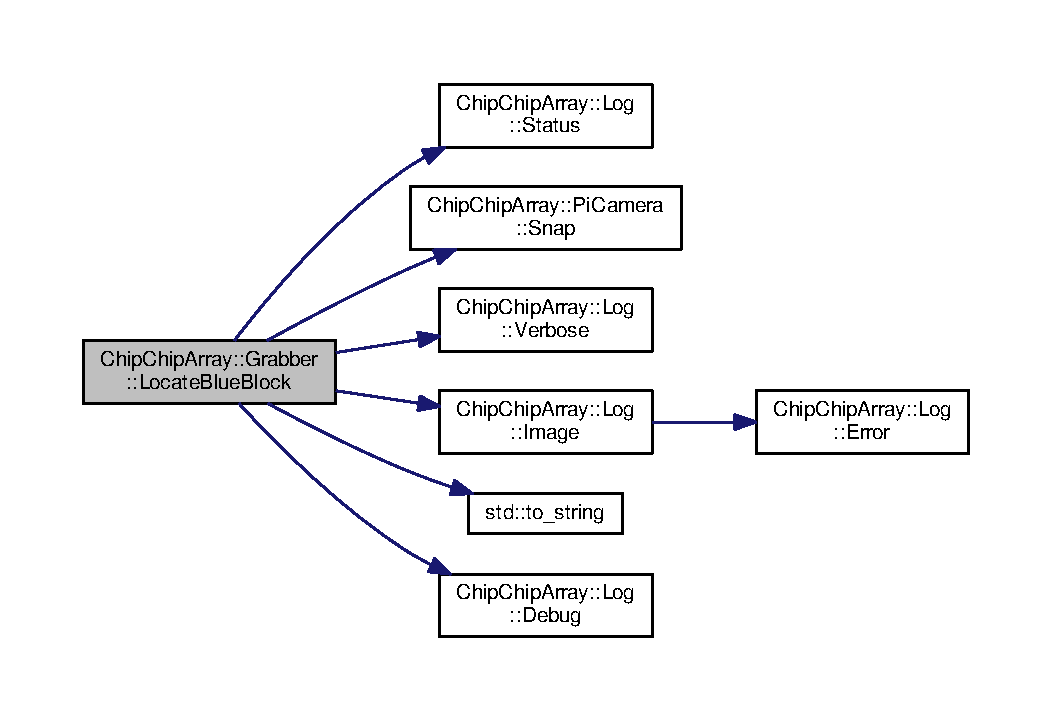
\includegraphics[width=350pt]{classChipChipArray_1_1Grabber_ab9b0d6a64b2c94c0d0f810a5ebeef6ec_cgraph}
\end{center}
\end{figure}




Here is the caller graph for this function\+:
\nopagebreak
\begin{figure}[H]
\begin{center}
\leavevmode
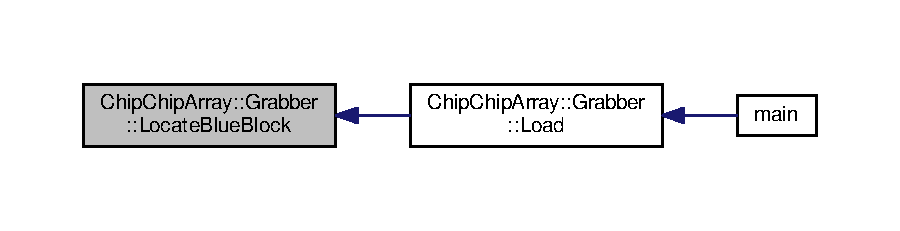
\includegraphics[width=350pt]{classChipChipArray_1_1Grabber_ab9b0d6a64b2c94c0d0f810a5ebeef6ec_icgraph}
\end{center}
\end{figure}




\subsection{Member Data Documentation}
\hypertarget{classChipChipArray_1_1Grabber_a726bcc2367a719cb84de92a981947622}{\index{Chip\+Chip\+Array\+::\+Grabber@{Chip\+Chip\+Array\+::\+Grabber}!cam@{cam}}
\index{cam@{cam}!Chip\+Chip\+Array\+::\+Grabber@{Chip\+Chip\+Array\+::\+Grabber}}
\subsubsection[{cam}]{\setlength{\rightskip}{0pt plus 5cm}{\bf Pi\+Camera} Chip\+Chip\+Array\+::\+Grabber\+::cam\hspace{0.3cm}{\ttfamily [protected]}}}\label{classChipChipArray_1_1Grabber_a726bcc2367a719cb84de92a981947622}
The Raspicam 

Definition at line \hyperlink{Grabber_8hpp_source_l00064}{64} of file \hyperlink{Grabber_8hpp_source}{Grabber.\+hpp}.

\hypertarget{classChipChipArray_1_1Grabber_a8afbaefae7c767c862fd1bf13968539b}{\index{Chip\+Chip\+Array\+::\+Grabber@{Chip\+Chip\+Array\+::\+Grabber}!side@{side}}
\index{side@{side}!Chip\+Chip\+Array\+::\+Grabber@{Chip\+Chip\+Array\+::\+Grabber}}
\subsubsection[{side}]{\setlength{\rightskip}{0pt plus 5cm}{\bf Side} Chip\+Chip\+Array\+::\+Grabber\+::side\hspace{0.3cm}{\ttfamily [protected]}}}\label{classChipChipArray_1_1Grabber_a8afbaefae7c767c862fd1bf13968539b}
The side from which the robot is coming (i.\+e., the side where the higher priority blocks are to be picked up. 

Definition at line \hyperlink{Grabber_8hpp_source_l00071}{71} of file \hyperlink{Grabber_8hpp_source}{Grabber.\+hpp}.

\hypertarget{classChipChipArray_1_1Grabber_ab57efe6e0b6f369b19528285a278d967}{\index{Chip\+Chip\+Array\+::\+Grabber@{Chip\+Chip\+Array\+::\+Grabber}!zone@{zone}}
\index{zone@{zone}!Chip\+Chip\+Array\+::\+Grabber@{Chip\+Chip\+Array\+::\+Grabber}}
\subsubsection[{zone}]{\setlength{\rightskip}{0pt plus 5cm}{\bf Zone} Chip\+Chip\+Array\+::\+Grabber\+::zone\hspace{0.3cm}{\ttfamily [protected]}}}\label{classChipChipArray_1_1Grabber_ab57efe6e0b6f369b19528285a278d967}
The zone in which blocks are being loaded. 

Definition at line \hyperlink{Grabber_8hpp_source_l00076}{76} of file \hyperlink{Grabber_8hpp_source}{Grabber.\+hpp}.



The documentation for this class was generated from the following file\+:\begin{DoxyCompactItemize}
\item 
src/\hyperlink{Grabber_8hpp}{Grabber.\+hpp}\end{DoxyCompactItemize}

\hypertarget{classChipChipArray_1_1Log}{\section{Chip\+Chip\+Array\+:\+:Log Class Reference}
\label{classChipChipArray_1_1Log}\index{Chip\+Chip\+Array\+::\+Log@{Chip\+Chip\+Array\+::\+Log}}
}


{\ttfamily \#include $<$Log.\+hpp$>$}

\subsection*{Public Member Functions}
\begin{DoxyCompactItemize}
\item 
\hyperlink{classChipChipArray_1_1Log_a2bd48afdb832567e94545e6dc2f6f4d5}{Log} ()
\item 
\hyperlink{classChipChipArray_1_1Log_a4cd28a821789b39e936a6e346329d65b}{Log} (auto dir, \hyperlink{definitions_8hpp_aa7380b6d694cab49f07aed6a7af592d9}{Log\+Mode} mode=\hyperlink{definitions_8hpp_aa7380b6d694cab49f07aed6a7af592d9a9dffbf69ffba8bc38bc4e01abf4b1675}{Log\+Mode\+::\+Text})
\item 
\hyperlink{classChipChipArray_1_1Log_a647df4da22b29d9d5a5ea32af3a1ed83}{$\sim$\+Log} ()
\item 
void \hyperlink{classChipChipArray_1_1Log_ac32b435af1577e4ebc67af2bdfea8eff}{Debug} (auto mesg)
\item 
void \hyperlink{classChipChipArray_1_1Log_aba7b7b0555f49f4dcf15f4b9fd3e6b34}{Error} (auto mesg)
\item 
void \hyperlink{classChipChipArray_1_1Log_a65bbab057c8b1453f9e4efcfee7522c4}{Image} (cv\+::\+Mat image, auto filename)
\item 
void \hyperlink{classChipChipArray_1_1Log_ad27a06a4561f2f59159bd8a7fc2fed3b}{Open} (auto dir, \hyperlink{definitions_8hpp_aa7380b6d694cab49f07aed6a7af592d9}{Log\+Mode} mode=\hyperlink{definitions_8hpp_aa7380b6d694cab49f07aed6a7af592d9a9dffbf69ffba8bc38bc4e01abf4b1675}{Log\+Mode\+::\+Text})
\item 
void \hyperlink{classChipChipArray_1_1Log_a66575b6e94c6112e4cefa5736cb996e0}{Status} (auto mesg)
\item 
void \hyperlink{classChipChipArray_1_1Log_a8849569720c26e335e7ef4dcb912170b}{Variable} (auto name, auto value)
\item 
void \hyperlink{classChipChipArray_1_1Log_a154a5f38d9c7a767693b242684a3d4d9}{Verbose} (auto mesg)
\end{DoxyCompactItemize}


\subsection{Detailed Description}
This class logs the text and images passed to it to specificed directory.

A \char`\"{}container\char`\"{} directory to which the class can write is passed in the constructor. When the \hyperlink{classChipChipArray_1_1Log}{Log} is initialized with \hyperlink{definitions_8hpp_aa7380b6d694cab49f07aed6a7af592d9a9dffbf69ffba8bc38bc4e01abf4b1675}{Log\+Mode\+::\+Text}, a new log file is created with a filename based on the time of initialization in the given directory. When initialized in \hyperlink{definitions_8hpp_aa7380b6d694cab49f07aed6a7af592d9ace7898536dd0e928d1640ee2ad531cc8}{Log\+Mode\+::\+Multi}, it will create a subdirectory in the given directory with a name based on time. In this new directory, a log file will be created. Images may later be stored in this directory with names based on the order in which they were saved.

This class D\+O\+E\+S N\+O\+T W\+O\+R\+K without compiling without a \char`\"{}\+L\+O\+G\char`\"{} definition (\#define L\+O\+G or -\/\+D\+L\+O\+G). 

Definition at line 34 of file Log.\+hpp.



\subsection{Constructor \& Destructor Documentation}
\hypertarget{classChipChipArray_1_1Log_a2bd48afdb832567e94545e6dc2f6f4d5}{\index{Chip\+Chip\+Array\+::\+Log@{Chip\+Chip\+Array\+::\+Log}!Log@{Log}}
\index{Log@{Log}!Chip\+Chip\+Array\+::\+Log@{Chip\+Chip\+Array\+::\+Log}}
\subsubsection[{Log}]{\setlength{\rightskip}{0pt plus 5cm}Chip\+Chip\+Array\+::\+Log\+::\+Log (
\begin{DoxyParamCaption}
{}
\end{DoxyParamCaption}
)\hspace{0.3cm}{\ttfamily [inline]}}}\label{classChipChipArray_1_1Log_a2bd48afdb832567e94545e6dc2f6f4d5}
Initializes \hyperlink{classChipChipArray_1_1Log}{Log} object but does not open log. \hyperlink{classChipChipArray_1_1Log_ad27a06a4561f2f59159bd8a7fc2fed3b}{Open()} must be called. 

Definition at line 40 of file Log.\+hpp.

\hypertarget{classChipChipArray_1_1Log_a4cd28a821789b39e936a6e346329d65b}{\index{Chip\+Chip\+Array\+::\+Log@{Chip\+Chip\+Array\+::\+Log}!Log@{Log}}
\index{Log@{Log}!Chip\+Chip\+Array\+::\+Log@{Chip\+Chip\+Array\+::\+Log}}
\subsubsection[{Log}]{\setlength{\rightskip}{0pt plus 5cm}Chip\+Chip\+Array\+::\+Log\+::\+Log (
\begin{DoxyParamCaption}
\item[{auto}]{dir, }
\item[{{\bf Log\+Mode}}]{mode = {\ttfamily {\bf Log\+Mode\+::\+Text}}}
\end{DoxyParamCaption}
)}}\label{classChipChipArray_1_1Log_a4cd28a821789b39e936a6e346329d65b}
Initializes the \hyperlink{classChipChipArray_1_1Log}{Log}.

A new log file is created in dir if \hyperlink{definitions_8hpp_aa7380b6d694cab49f07aed6a7af592d9a9dffbf69ffba8bc38bc4e01abf4b1675}{Log\+Mode\+::\+Text} is given. The file will have a name based on the current date and time. If \hyperlink{definitions_8hpp_aa7380b6d694cab49f07aed6a7af592d9ace7898536dd0e928d1640ee2ad531cc8}{Log\+Mode\+::\+Multi} is given, a new directory is created, and a log file with a name based on the current date and time is created inside it.


\begin{DoxyParams}{Parameters}
{\em dir} & the directory for the newly created logfile/folder\\
\hline
{\em mode} & the Log\+Mode \\
\hline
\end{DoxyParams}


Definition at line 186 of file Log.\+hpp.



Here is the call graph for this function\+:
\nopagebreak
\begin{figure}[H]
\begin{center}
\leavevmode
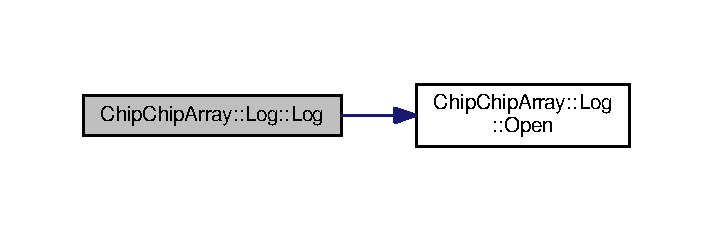
\includegraphics[width=342pt]{classChipChipArray_1_1Log_a4cd28a821789b39e936a6e346329d65b_cgraph}
\end{center}
\end{figure}


\hypertarget{classChipChipArray_1_1Log_a647df4da22b29d9d5a5ea32af3a1ed83}{\index{Chip\+Chip\+Array\+::\+Log@{Chip\+Chip\+Array\+::\+Log}!````~Log@{$\sim$\+Log}}
\index{````~Log@{$\sim$\+Log}!Chip\+Chip\+Array\+::\+Log@{Chip\+Chip\+Array\+::\+Log}}
\subsubsection[{$\sim$\+Log}]{\setlength{\rightskip}{0pt plus 5cm}Chip\+Chip\+Array\+::\+Log\+::$\sim$\+Log (
\begin{DoxyParamCaption}
{}
\end{DoxyParamCaption}
)}}\label{classChipChipArray_1_1Log_a647df4da22b29d9d5a5ea32af3a1ed83}
Destroys the \hyperlink{classChipChipArray_1_1Log}{Log} and closes the logfile. 

Definition at line 192 of file Log.\+hpp.



\subsection{Member Function Documentation}
\hypertarget{classChipChipArray_1_1Log_ac32b435af1577e4ebc67af2bdfea8eff}{\index{Chip\+Chip\+Array\+::\+Log@{Chip\+Chip\+Array\+::\+Log}!Debug@{Debug}}
\index{Debug@{Debug}!Chip\+Chip\+Array\+::\+Log@{Chip\+Chip\+Array\+::\+Log}}
\subsubsection[{Debug}]{\setlength{\rightskip}{0pt plus 5cm}void Chip\+Chip\+Array\+::\+Log\+::\+Debug (
\begin{DoxyParamCaption}
\item[{auto}]{mesg}
\end{DoxyParamCaption}
)}}\label{classChipChipArray_1_1Log_ac32b435af1577e4ebc67af2bdfea8eff}
Writes \char`\"{}\+D\+E\+B\+U\+G\+: \char`\"{} to the log file along with the message passed. Should be used for generic debugging information. If recording the value of a variable in the \hyperlink{classChipChipArray_1_1Log}{Log} is desired, use the function \hyperlink{classChipChipArray_1_1Log_a8849569720c26e335e7ef4dcb912170b}{Variable()} instead.


\begin{DoxyParams}{Parameters}
{\em mesg} & the message to record in the logfile \\
\hline
\end{DoxyParams}


Definition at line 204 of file Log.\+hpp.



Here is the caller graph for this function\+:
\nopagebreak
\begin{figure}[H]
\begin{center}
\leavevmode
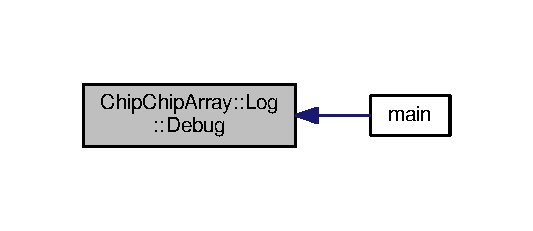
\includegraphics[width=256pt]{classChipChipArray_1_1Log_ac32b435af1577e4ebc67af2bdfea8eff_icgraph}
\end{center}
\end{figure}


\hypertarget{classChipChipArray_1_1Log_aba7b7b0555f49f4dcf15f4b9fd3e6b34}{\index{Chip\+Chip\+Array\+::\+Log@{Chip\+Chip\+Array\+::\+Log}!Error@{Error}}
\index{Error@{Error}!Chip\+Chip\+Array\+::\+Log@{Chip\+Chip\+Array\+::\+Log}}
\subsubsection[{Error}]{\setlength{\rightskip}{0pt plus 5cm}void Chip\+Chip\+Array\+::\+Log\+::\+Error (
\begin{DoxyParamCaption}
\item[{auto}]{mesg}
\end{DoxyParamCaption}
)}}\label{classChipChipArray_1_1Log_aba7b7b0555f49f4dcf15f4b9fd3e6b34}
Writes \char`\"{}\+E\+R\+R\+O\+R\+: \char`\"{} to the log file. Should only be use when an exception is thrown.


\begin{DoxyParams}{Parameters}
{\em mesg} & the message to record in the log \\
\hline
\end{DoxyParams}


Definition at line 215 of file Log.\+hpp.



Here is the caller graph for this function\+:
\nopagebreak
\begin{figure}[H]
\begin{center}
\leavevmode
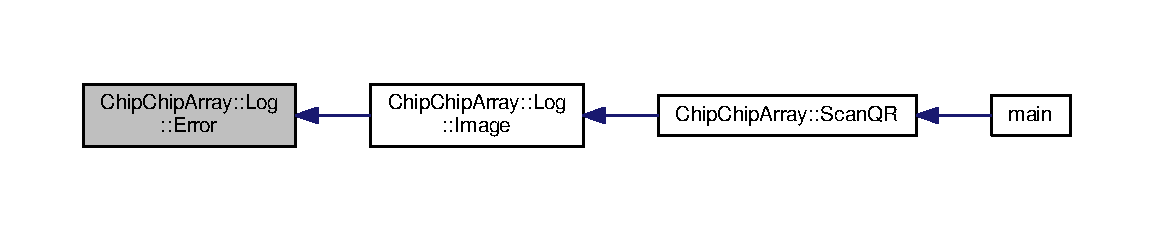
\includegraphics[width=350pt]{classChipChipArray_1_1Log_aba7b7b0555f49f4dcf15f4b9fd3e6b34_icgraph}
\end{center}
\end{figure}


\hypertarget{classChipChipArray_1_1Log_a65bbab057c8b1453f9e4efcfee7522c4}{\index{Chip\+Chip\+Array\+::\+Log@{Chip\+Chip\+Array\+::\+Log}!Image@{Image}}
\index{Image@{Image}!Chip\+Chip\+Array\+::\+Log@{Chip\+Chip\+Array\+::\+Log}}
\subsubsection[{Image}]{\setlength{\rightskip}{0pt plus 5cm}void Chip\+Chip\+Array\+::\+Log\+::\+Image (
\begin{DoxyParamCaption}
\item[{cv\+::\+Mat}]{image, }
\item[{auto}]{filename}
\end{DoxyParamCaption}
)}}\label{classChipChipArray_1_1Log_a65bbab057c8b1453f9e4efcfee7522c4}
Creates a bitmap image in the subdirectory created by the \hyperlink{classChipChipArray_1_1Log}{Log} during initialization. Does nothing if \hyperlink{definitions_8hpp_aa7380b6d694cab49f07aed6a7af592d9a9dffbf69ffba8bc38bc4e01abf4b1675}{Log\+Mode\+::\+Text} was passed in the constructor.


\begin{DoxyParams}{Parameters}
{\em image} & the image to save \\
\hline
{\em filename} & the filename for the saved image \\
\hline
\end{DoxyParams}


Definition at line 226 of file Log.\+hpp.



Here is the call graph for this function\+:
\nopagebreak
\begin{figure}[H]
\begin{center}
\leavevmode
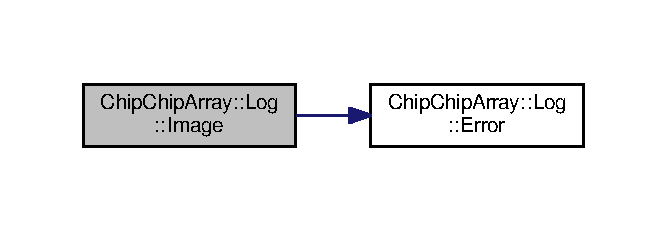
\includegraphics[width=320pt]{classChipChipArray_1_1Log_a65bbab057c8b1453f9e4efcfee7522c4_cgraph}
\end{center}
\end{figure}




Here is the caller graph for this function\+:
\nopagebreak
\begin{figure}[H]
\begin{center}
\leavevmode
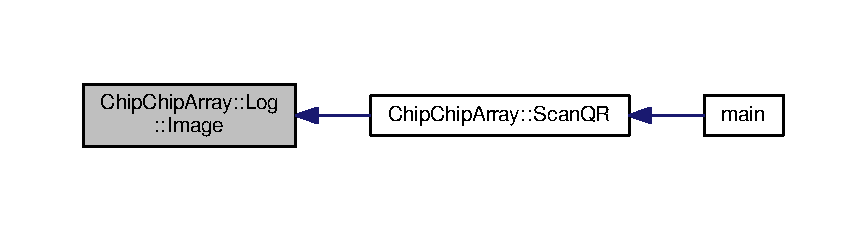
\includegraphics[width=350pt]{classChipChipArray_1_1Log_a65bbab057c8b1453f9e4efcfee7522c4_icgraph}
\end{center}
\end{figure}


\hypertarget{classChipChipArray_1_1Log_ad27a06a4561f2f59159bd8a7fc2fed3b}{\index{Chip\+Chip\+Array\+::\+Log@{Chip\+Chip\+Array\+::\+Log}!Open@{Open}}
\index{Open@{Open}!Chip\+Chip\+Array\+::\+Log@{Chip\+Chip\+Array\+::\+Log}}
\subsubsection[{Open}]{\setlength{\rightskip}{0pt plus 5cm}void Chip\+Chip\+Array\+::\+Log\+::\+Open (
\begin{DoxyParamCaption}
\item[{auto}]{dir, }
\item[{{\bf Log\+Mode}}]{mode = {\ttfamily {\bf Log\+Mode\+::\+Text}}}
\end{DoxyParamCaption}
)}}\label{classChipChipArray_1_1Log_ad27a06a4561f2f59159bd8a7fc2fed3b}


Definition at line 246 of file Log.\+hpp.



Here is the caller graph for this function\+:
\nopagebreak
\begin{figure}[H]
\begin{center}
\leavevmode
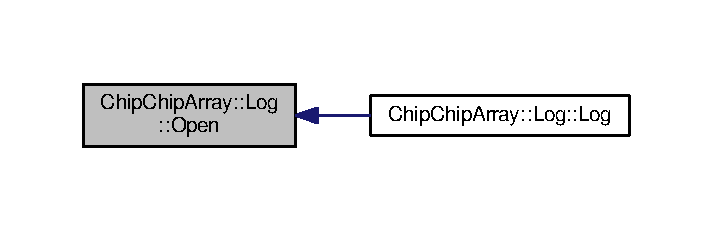
\includegraphics[width=342pt]{classChipChipArray_1_1Log_ad27a06a4561f2f59159bd8a7fc2fed3b_icgraph}
\end{center}
\end{figure}


\hypertarget{classChipChipArray_1_1Log_a66575b6e94c6112e4cefa5736cb996e0}{\index{Chip\+Chip\+Array\+::\+Log@{Chip\+Chip\+Array\+::\+Log}!Status@{Status}}
\index{Status@{Status}!Chip\+Chip\+Array\+::\+Log@{Chip\+Chip\+Array\+::\+Log}}
\subsubsection[{Status}]{\setlength{\rightskip}{0pt plus 5cm}void Chip\+Chip\+Array\+::\+Log\+::\+Status (
\begin{DoxyParamCaption}
\item[{auto}]{mesg}
\end{DoxyParamCaption}
)}}\label{classChipChipArray_1_1Log_a66575b6e94c6112e4cefa5736cb996e0}
Writes \char`\"{}\+S\+T\+A\+T\+U\+S\+: \char`\"{} to the log file. Should be used when recording the status or state of the program. It should not be used to record microalgorithmic changes. Use \hyperlink{classChipChipArray_1_1Log_a154a5f38d9c7a767693b242684a3d4d9}{Verbose()} for these instead.


\begin{DoxyParams}{Parameters}
{\em mesg} & the message to record in the logfile \\
\hline
\end{DoxyParams}


Definition at line 289 of file Log.\+hpp.



Here is the caller graph for this function\+:
\nopagebreak
\begin{figure}[H]
\begin{center}
\leavevmode
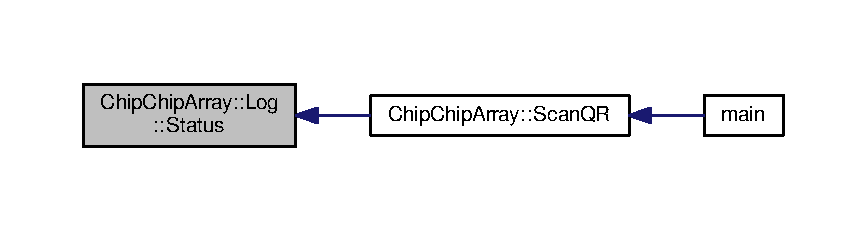
\includegraphics[width=350pt]{classChipChipArray_1_1Log_a66575b6e94c6112e4cefa5736cb996e0_icgraph}
\end{center}
\end{figure}


\hypertarget{classChipChipArray_1_1Log_a8849569720c26e335e7ef4dcb912170b}{\index{Chip\+Chip\+Array\+::\+Log@{Chip\+Chip\+Array\+::\+Log}!Variable@{Variable}}
\index{Variable@{Variable}!Chip\+Chip\+Array\+::\+Log@{Chip\+Chip\+Array\+::\+Log}}
\subsubsection[{Variable}]{\setlength{\rightskip}{0pt plus 5cm}void Chip\+Chip\+Array\+::\+Log\+::\+Variable (
\begin{DoxyParamCaption}
\item[{auto}]{name, }
\item[{auto}]{value}
\end{DoxyParamCaption}
)}}\label{classChipChipArray_1_1Log_a8849569720c26e335e7ef4dcb912170b}
Writes \char`\"{}\+V\+A\+R\+I\+A\+B\+L\+E\+: \char`\"{} to the log file. Should be used whenever recording the value of a variable is desired.


\begin{DoxyParams}{Parameters}
{\em name} & the variable name to record \\
\hline
{\em value} & the variable value to record \\
\hline
\end{DoxyParams}


Definition at line 300 of file Log.\+hpp.



Here is the caller graph for this function\+:
\nopagebreak
\begin{figure}[H]
\begin{center}
\leavevmode
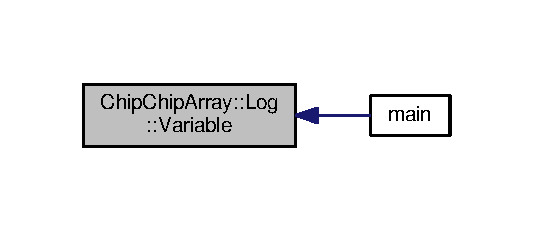
\includegraphics[width=256pt]{classChipChipArray_1_1Log_a8849569720c26e335e7ef4dcb912170b_icgraph}
\end{center}
\end{figure}


\hypertarget{classChipChipArray_1_1Log_a154a5f38d9c7a767693b242684a3d4d9}{\index{Chip\+Chip\+Array\+::\+Log@{Chip\+Chip\+Array\+::\+Log}!Verbose@{Verbose}}
\index{Verbose@{Verbose}!Chip\+Chip\+Array\+::\+Log@{Chip\+Chip\+Array\+::\+Log}}
\subsubsection[{Verbose}]{\setlength{\rightskip}{0pt plus 5cm}void Chip\+Chip\+Array\+::\+Log\+::\+Verbose (
\begin{DoxyParamCaption}
\item[{auto}]{mesg}
\end{DoxyParamCaption}
)}}\label{classChipChipArray_1_1Log_a154a5f38d9c7a767693b242684a3d4d9}
Writes \char`\"{}\+V\+E\+R\+B\+O\+S\+E\+: \char`\"{} to the log file. Should only be used for recording small, specific portions of code. To record a change in the more general state of the program, use \hyperlink{classChipChipArray_1_1Log_a66575b6e94c6112e4cefa5736cb996e0}{Status()} instead.


\begin{DoxyParams}{Parameters}
{\em mesg} & the message to record in the logfile \\
\hline
\end{DoxyParams}


Definition at line 312 of file Log.\+hpp.



Here is the caller graph for this function\+:
\nopagebreak
\begin{figure}[H]
\begin{center}
\leavevmode
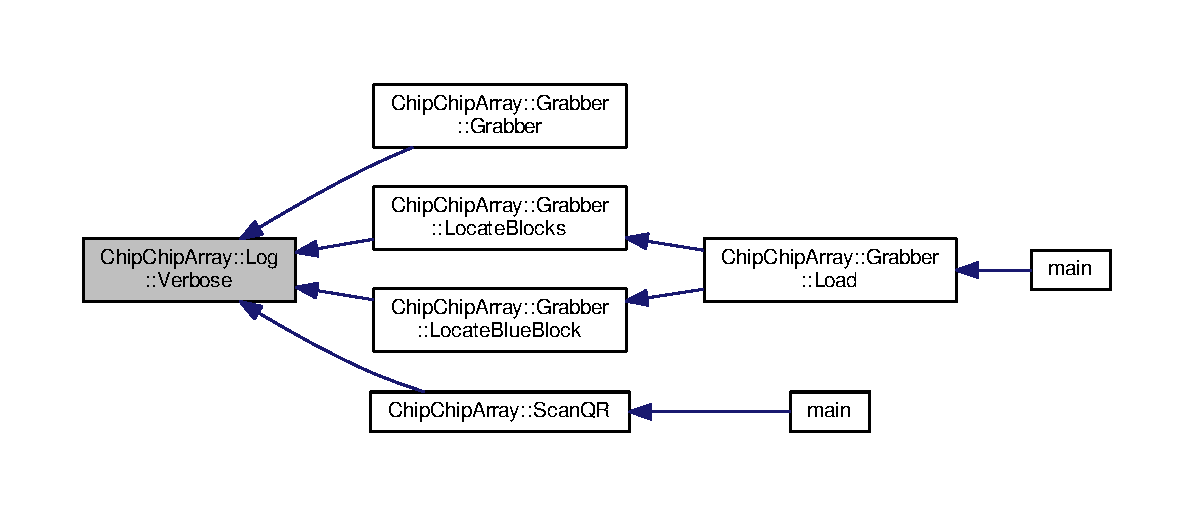
\includegraphics[width=350pt]{classChipChipArray_1_1Log_a154a5f38d9c7a767693b242684a3d4d9_icgraph}
\end{center}
\end{figure}




The documentation for this class was generated from the following file\+:\begin{DoxyCompactItemize}
\item 
src/\hyperlink{Log_8hpp}{Log.\+hpp}\end{DoxyCompactItemize}

\hypertarget{classChipChipArray_1_1PiCamera}{\section{Chip\+Chip\+Array\+:\+:Pi\+Camera Class Reference}
\label{classChipChipArray_1_1PiCamera}\index{Chip\+Chip\+Array\+::\+Pi\+Camera@{Chip\+Chip\+Array\+::\+Pi\+Camera}}
}


{\ttfamily \#include $<$Pi\+Camera.\+hpp$>$}

\subsection*{Public Member Functions}
\begin{DoxyCompactItemize}
\item 
\hyperlink{classChipChipArray_1_1PiCamera_a5910a3284877677decb6529d88e43487}{Pi\+Camera} ()
\item 
\hyperlink{classChipChipArray_1_1PiCamera_a0a4480e9e7475ae7af9a7523239caf8d}{Pi\+Camera} (bool use\+Color)
\item 
void \hyperlink{classChipChipArray_1_1PiCamera_a38f8205921d6deec5a2c360ea7d24cc5}{Close} ()
\item 
cv\+::\+Mat \hyperlink{classChipChipArray_1_1PiCamera_a58fb0de02570dce9a9cb60a1a04fb84f}{Snap} ()
\end{DoxyCompactItemize}


\subsection{Detailed Description}
This class is a basic wrapper to allow the Raspicam to interface with Open\+C\+V. It uses another wrapper class, Raspicam, provided by Cédric Verstraeten (\href{https://github.com/cedricve/raspicam}{\tt https\+://github.\+com/cedricve/raspicam}). 

Definition at line \hyperlink{PiCamera_8hpp_source_l00024}{24} of file \hyperlink{PiCamera_8hpp_source}{Pi\+Camera.\+hpp}.



\subsection{Constructor \& Destructor Documentation}
\hypertarget{classChipChipArray_1_1PiCamera_a5910a3284877677decb6529d88e43487}{\index{Chip\+Chip\+Array\+::\+Pi\+Camera@{Chip\+Chip\+Array\+::\+Pi\+Camera}!Pi\+Camera@{Pi\+Camera}}
\index{Pi\+Camera@{Pi\+Camera}!Chip\+Chip\+Array\+::\+Pi\+Camera@{Chip\+Chip\+Array\+::\+Pi\+Camera}}
\subsubsection[{Pi\+Camera}]{\setlength{\rightskip}{0pt plus 5cm}Chip\+Chip\+Array\+::\+Pi\+Camera\+::\+Pi\+Camera (
\begin{DoxyParamCaption}
{}
\end{DoxyParamCaption}
)\hspace{0.3cm}{\ttfamily [inline]}}}\label{classChipChipArray_1_1PiCamera_a5910a3284877677decb6529d88e43487}
Opens the camera and configures it for color images. 

Definition at line \hyperlink{PiCamera_8hpp_source_l00029}{29} of file \hyperlink{PiCamera_8hpp_source}{Pi\+Camera.\+hpp}.


\begin{DoxyCode}
00029 : \hyperlink{classChipChipArray_1_1PiCamera_a5910a3284877677decb6529d88e43487}{PiCamera}(\textcolor{keyword}{true}) \{\};
\end{DoxyCode}
\hypertarget{classChipChipArray_1_1PiCamera_a0a4480e9e7475ae7af9a7523239caf8d}{\index{Chip\+Chip\+Array\+::\+Pi\+Camera@{Chip\+Chip\+Array\+::\+Pi\+Camera}!Pi\+Camera@{Pi\+Camera}}
\index{Pi\+Camera@{Pi\+Camera}!Chip\+Chip\+Array\+::\+Pi\+Camera@{Chip\+Chip\+Array\+::\+Pi\+Camera}}
\subsubsection[{Pi\+Camera}]{\setlength{\rightskip}{0pt plus 5cm}Chip\+Chip\+Array\+::\+Pi\+Camera\+::\+Pi\+Camera (
\begin{DoxyParamCaption}
\item[{bool}]{use\+Color}
\end{DoxyParamCaption}
)}}\label{classChipChipArray_1_1PiCamera_a0a4480e9e7475ae7af9a7523239caf8d}
Opens the camera.


\begin{DoxyParams}{Parameters}
{\em use\+Color} & Specifices whether camera should make color images. T\+R\+U\+E = color, F\+A\+L\+S\+E = grayscale. \\
\hline
\end{DoxyParams}


Definition at line \hyperlink{PiCamera_8hpp_source_l00059}{59} of file \hyperlink{PiCamera_8hpp_source}{Pi\+Camera.\+hpp}.


\begin{DoxyCode}
00059                                     \{
00060         cam.set(CV\_CAP\_PROP\_FORMAT, (useColor ? CV\_16UC3 : CV\_16UC1));
00061         cam.open();
00062         usleep(500000);  \textcolor{comment}{// required to allow camera time to adjust!}
00063     \}
\end{DoxyCode}


\subsection{Member Function Documentation}
\hypertarget{classChipChipArray_1_1PiCamera_a38f8205921d6deec5a2c360ea7d24cc5}{\index{Chip\+Chip\+Array\+::\+Pi\+Camera@{Chip\+Chip\+Array\+::\+Pi\+Camera}!Close@{Close}}
\index{Close@{Close}!Chip\+Chip\+Array\+::\+Pi\+Camera@{Chip\+Chip\+Array\+::\+Pi\+Camera}}
\subsubsection[{Close}]{\setlength{\rightskip}{0pt plus 5cm}void Chip\+Chip\+Array\+::\+Pi\+Camera\+::\+Close (
\begin{DoxyParamCaption}
{}
\end{DoxyParamCaption}
)}}\label{classChipChipArray_1_1PiCamera_a38f8205921d6deec5a2c360ea7d24cc5}
Closes connection to camera. 

Definition at line \hyperlink{PiCamera_8hpp_source_l00065}{65} of file \hyperlink{PiCamera_8hpp_source}{Pi\+Camera.\+hpp}.


\begin{DoxyCode}
00065                          \{
00066         cam.release();
00067     \}
\end{DoxyCode}


Here is the caller graph for this function\+:
\nopagebreak
\begin{figure}[H]
\begin{center}
\leavevmode
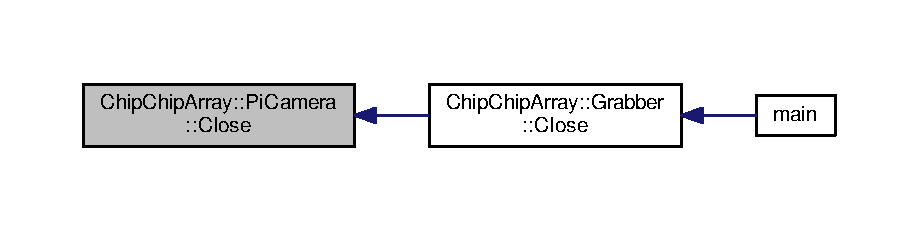
\includegraphics[width=350pt]{classChipChipArray_1_1PiCamera_a38f8205921d6deec5a2c360ea7d24cc5_icgraph}
\end{center}
\end{figure}


\hypertarget{classChipChipArray_1_1PiCamera_a58fb0de02570dce9a9cb60a1a04fb84f}{\index{Chip\+Chip\+Array\+::\+Pi\+Camera@{Chip\+Chip\+Array\+::\+Pi\+Camera}!Snap@{Snap}}
\index{Snap@{Snap}!Chip\+Chip\+Array\+::\+Pi\+Camera@{Chip\+Chip\+Array\+::\+Pi\+Camera}}
\subsubsection[{Snap}]{\setlength{\rightskip}{0pt plus 5cm}cv\+::\+Mat Chip\+Chip\+Array\+::\+Pi\+Camera\+::\+Snap (
\begin{DoxyParamCaption}
{}
\end{DoxyParamCaption}
)}}\label{classChipChipArray_1_1PiCamera_a58fb0de02570dce9a9cb60a1a04fb84f}
Makes picture.

\begin{DoxyReturn}{Returns}
Open\+C\+V Mat object (i.\+e., an image) from the camera 
\end{DoxyReturn}


Definition at line \hyperlink{PiCamera_8hpp_source_l00069}{69} of file \hyperlink{PiCamera_8hpp_source}{Pi\+Camera.\+hpp}.


\begin{DoxyCode}
00069                          \{
00070         \textcolor{keywordflow}{if}(!cam.isOpened()) \textcolor{keywordflow}{throw} std::runtime\_error(\textcolor{stringliteral}{"Camera "}
00071                 \textcolor{stringliteral}{"is not open!"});
00072 
00073         cv::Mat image;
00074         cam.grab();
00075         cam.retrieve(image);
00076         \textcolor{keywordflow}{return} image;
00077     \}
\end{DoxyCode}


Here is the caller graph for this function\+:
\nopagebreak
\begin{figure}[H]
\begin{center}
\leavevmode
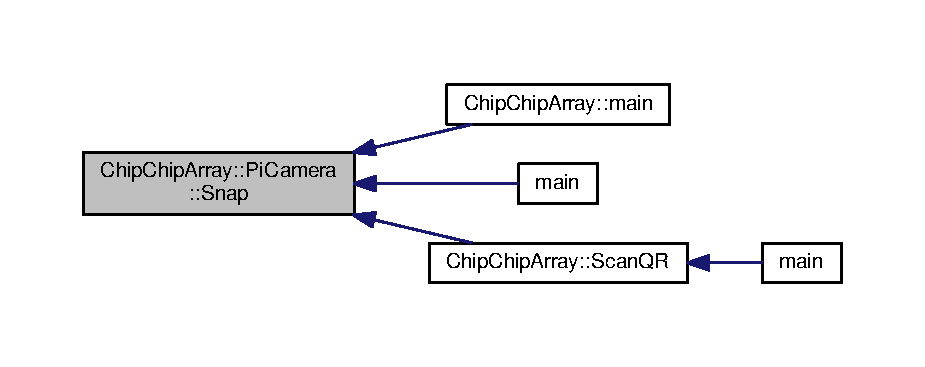
\includegraphics[width=350pt]{classChipChipArray_1_1PiCamera_a58fb0de02570dce9a9cb60a1a04fb84f_icgraph}
\end{center}
\end{figure}




The documentation for this class was generated from the following file\+:\begin{DoxyCompactItemize}
\item 
src/\hyperlink{PiCamera_8hpp}{Pi\+Camera.\+hpp}\end{DoxyCompactItemize}

\chapter{File Documentation}
\hypertarget{doxygen_8config}{\section{etc/doxygen.config File Reference}
\label{doxygen_8config}\index{etc/doxygen.\+config@{etc/doxygen.\+config}}
}

\hypertarget{doxygen_8config_source}{\section{doxygen.\+config}
\label{doxygen_8config_source}\index{etc/doxygen.\+config@{etc/doxygen.\+config}}
}

\begin{DoxyCode}
00001 PROJECT\_NAME = "The Automatic Vasospasm Detection Application"
00002 
00003 INPUT = src/ etc/doxygen.config makefile
00004 OUTPUT\_DIRECTORY = doc/
00005 
00006 GENERATE\_HTML = YES
00007 GENERATE\_RTF = YES
00008 GENERATE\_LATEX = YES
00009 GENERATE\_MAN = YES
00010 GENERATE\_XML = NO
00011 GENERATE\_DOCBOOK = NO
00012 
00013 USE\_PDF\_LATEX = YES
00014 USE\_PDF\_HYPERLINKS = YES
00015 
00016 RECURSIVE = YES
00017 SOURCE\_BROWSER = YES
00018 SOURCE\_TOOLTIPS = YES
00019 EXTRACT\_ALL = YES
00020 DISABLE\_INDEX = NO
00021 GENERATE\_TREEVIEW = YES
00022 SEARCHENGINE = YES
00023 SERVER\_BASED\_SEARCH = NO
00024 USE\_MDFILE\_AS\_MAINPAGE = README.md
00025 
00026 LATEX\_SOURCE\_CODE = YES
00027 STRIP\_CODE\_COMMENTS = YES
00028 INLINE\_SOURCES = YES
00029 
00030 HAVE\_DOT = YES
00031 CALL\_GRAPH = YES
00032 CALLER\_GRAPH = YES
\end{DoxyCode}

\hypertarget{makefile}{\section{makefile File Reference}
\label{makefile}\index{makefile@{makefile}}
}

\hypertarget{makefile_source}{\section{makefile}
}

\begin{DoxyCode}
00001 GCC = g++-4.9
00002 ARM = -L/usr/local/lib -lwiringPi
00003 CPPFLAGS = -g -std=gnu++14
00004 CVFLAGS = -lraspicam -lraspicam\_cv -lmmal -lmmal\_core -lmmal\_util -lzbar -lopencv\_core
       -lopencv\_highgui -lopencv\_imgproc
00005 LOG = -DLOG
00006 
00007 export LIBRARY\_PATH=/opt/vc/lib:/usr/lib/arm-linux-gnueabihf
00008 
00009 arm:
00010    $(GCC) src/dark\_magic.cpp -o bin/arm $(ARM) $(CPPFLAGS)
00011 
00012 block-test:
00013    $(GCC) src/cv\_shape.cpp -o bin/cvshape $(CVFLAGS) $(CPPFLAGS)
00014 
00015 channel-test:
00016    $(GCC) src/cv\_channel\_test.cpp -o bin/channeltest $(CVFLAGS) $(CPPFLAGS)
00017 
00018 
00019 comp:
00020    $(GCC) src/main.cpp -o bin/main $(CVFLAGS) $(CPPFLAGS) $(ARM) -lpthread
00021 
00022 configure:
00023    sudo apt-get install -y libopencv-dev libzbar-dev cmake doxygen libgl1-meda-dri
00024    git clone https://github.com/cedricve/raspicam
00025    cd raspicam; mkdir build; cd build; cmake ..; make; sudo make install; sudo ldconfig;
00026    sudo rm -r raspicam
00027    mkdir docs
00028 
00029 cv-test:
00030    $(GCC) src/cv\_test.cpp -o bin/cvtest $(CVFLAGS) $(CPPFLAGS) $(LOG)
00031 
00032 img:
00033    $(GCC) src/img.cpp -o bin/img $(CVFLAGS) $(CPPFLAGS)
00034 
00035 jacob-algorithm-test:
00036    $(GCC) src/jacob\_alg\_test.cpp -o bin/jacobalgtest $(CVFLAGS) $(CPPFLAGS)
00037 
00038 loading-test:
00039    $(GCC) src/loading\_test.cpp -o bin/loadingtest $(CPPFLAGS) $(LOG) $(ARM) $(CVFLAGS)
00040 
00041 log-test:
00042    $(GCC) src/log\_test.cpp -o bin/logtest $(CPPFLAGS) $(LOG)
00043 
00044 net-cv-hue-test:
00045    $(GCC) src/cv\_hue.cpp -o bin/cvhue $(CPPFLAGS) $(CVFLAGS)
00046 
00047 net-qr-test:
00048    $(GCC) src/net\_qr\_test.cpp -o bin/netqrtest $(CPPFLAGS) $(CVFLAGS)
00049 
00050 qr-test:
00051    $(GCC) src/qr\_test.cpp -o bin/qrtest $(CPPFLAGS) $(CVFLAGS) $(LOG)
00052 
00053 servotrip:
00054    $(GCC) src/main.cpp -o bin/servotrip $(CPPFLAGS) $(ARM)
00055 
00056 docs:
00057    rm -r doc/
00058    doxygen etc/doxygen.config
00059    cd doc/latex; make pdf;
00060    git reset
00061    git add doc/.
00062    git commit -m "Updated documentation."
00063    git push
00064 
00065 count:
00066    grep -r "src/" -e "Samuel Andrew Wisner" -l | xargs wc -l  # works assuming there's no
       subdirectories
\end{DoxyCode}

\hypertarget{Adafruit__PWMServoDriver_8cpp}{\section{src/\+Adafruit\+\_\+\+P\+W\+M\+Servo\+Driver.cpp File Reference}
\label{Adafruit__PWMServoDriver_8cpp}\index{src/\+Adafruit\+\_\+\+P\+W\+M\+Servo\+Driver.\+cpp@{src/\+Adafruit\+\_\+\+P\+W\+M\+Servo\+Driver.\+cpp}}
}
{\ttfamily \#include \char`\"{}Adafruit\+\_\+\+P\+W\+M\+Servo\+Driver.\+h\char`\"{}}\\*
Include dependency graph for Adafruit\+\_\+\+P\+W\+M\+Servo\+Driver.\+cpp\+:
\nopagebreak
\begin{figure}[H]
\begin{center}
\leavevmode
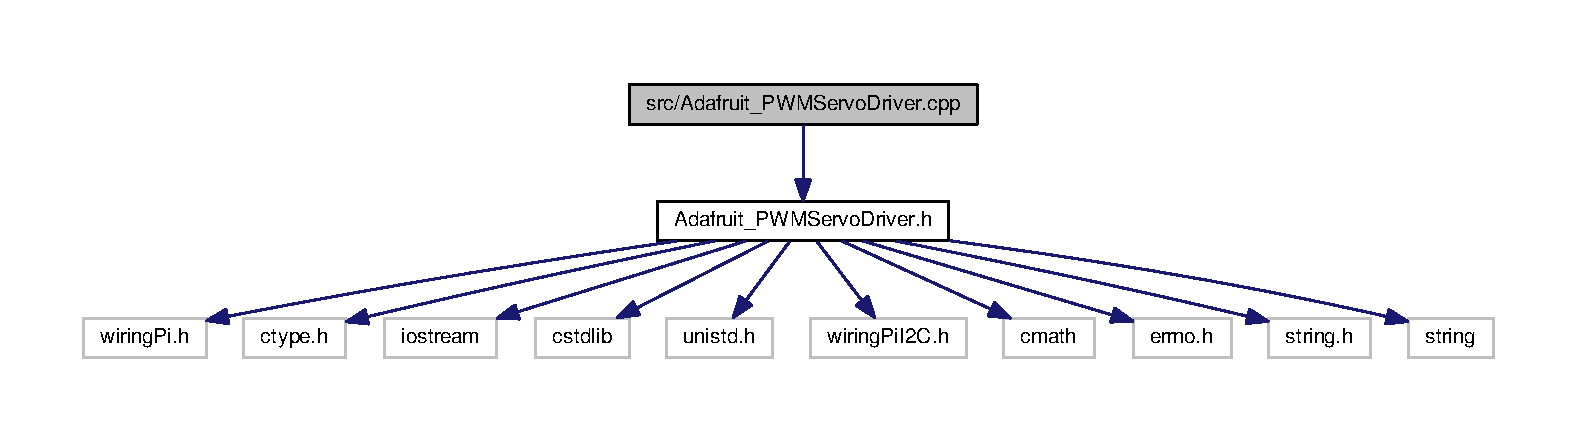
\includegraphics[width=350pt]{Adafruit__PWMServoDriver_8cpp__incl}
\end{center}
\end{figure}
This graph shows which files directly or indirectly include this file\+:
\nopagebreak
\begin{figure}[H]
\begin{center}
\leavevmode
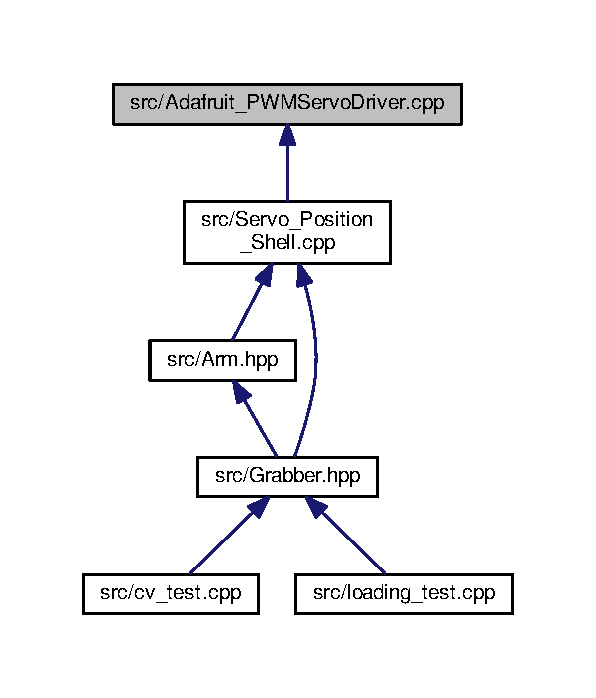
\includegraphics[width=333pt]{Adafruit__PWMServoDriver_8cpp__dep__incl}
\end{center}
\end{figure}
\subsection*{Macros}
\begin{DoxyCompactItemize}
\item 
\#define \hyperlink{Adafruit__PWMServoDriver_8cpp_a818989cbf7f37dae193fbb28b2d3976a}{E\+N\+A\+B\+L\+E\+\_\+\+D\+E\+B\+U\+G\+\_\+\+O\+U\+T\+P\+U\+T}~false
\end{DoxyCompactItemize}


\subsection{Macro Definition Documentation}
\hypertarget{Adafruit__PWMServoDriver_8cpp_a818989cbf7f37dae193fbb28b2d3976a}{\index{Adafruit\+\_\+\+P\+W\+M\+Servo\+Driver.\+cpp@{Adafruit\+\_\+\+P\+W\+M\+Servo\+Driver.\+cpp}!E\+N\+A\+B\+L\+E\+\_\+\+D\+E\+B\+U\+G\+\_\+\+O\+U\+T\+P\+U\+T@{E\+N\+A\+B\+L\+E\+\_\+\+D\+E\+B\+U\+G\+\_\+\+O\+U\+T\+P\+U\+T}}
\index{E\+N\+A\+B\+L\+E\+\_\+\+D\+E\+B\+U\+G\+\_\+\+O\+U\+T\+P\+U\+T@{E\+N\+A\+B\+L\+E\+\_\+\+D\+E\+B\+U\+G\+\_\+\+O\+U\+T\+P\+U\+T}!Adafruit\+\_\+\+P\+W\+M\+Servo\+Driver.\+cpp@{Adafruit\+\_\+\+P\+W\+M\+Servo\+Driver.\+cpp}}
\subsubsection[{E\+N\+A\+B\+L\+E\+\_\+\+D\+E\+B\+U\+G\+\_\+\+O\+U\+T\+P\+U\+T}]{\setlength{\rightskip}{0pt plus 5cm}\#define E\+N\+A\+B\+L\+E\+\_\+\+D\+E\+B\+U\+G\+\_\+\+O\+U\+T\+P\+U\+T~false}}\label{Adafruit__PWMServoDriver_8cpp_a818989cbf7f37dae193fbb28b2d3976a}


Definition at line 27 of file Adafruit\+\_\+\+P\+W\+M\+Servo\+Driver.\+cpp.


\hypertarget{Adafruit__PWMServoDriver_8cpp_source}{\section{Adafruit\+\_\+\+P\+W\+M\+Servo\+Driver.\+cpp}
\label{Adafruit__PWMServoDriver_8cpp_source}\index{src/\+Adafruit\+\_\+\+P\+W\+M\+Servo\+Driver.\+cpp@{src/\+Adafruit\+\_\+\+P\+W\+M\+Servo\+Driver.\+cpp}}
}

\begin{DoxyCode}
00001 
00009 \textcolor{comment}{/* File: Adafruit\_PWMServoDriver.cpp}
00010 \textcolor{comment}{ * Credit to Limor Fried/Ladyada for PWM servo driver code. }
00011 \textcolor{comment}{ * Editted by: Nickolas Neely for ChipChipArray Raspberry Pi }
00012 \textcolor{comment}{ */}
00013 
00014 \textcolor{comment}{/*************************************************** }
00015 \textcolor{comment}{  This is a library for our Adafruit 16-channel PWM & Servo driver}
00016 \textcolor{comment}{}
00017 \textcolor{comment}{  Pick one up today in the adafruit shop!}
00018 \textcolor{comment}{  ------> http://www.adafruit.com/products/815}
00019 \textcolor{comment}{}
00020 \textcolor{comment}{  These displays use I2C to communicate, 2 pins are required to  }
00021 \textcolor{comment}{  interface. For Arduino UNOs, thats SCL -> Analog 5, SDA -> Analog 4}
00022 \textcolor{comment}{}
00023 \textcolor{comment}{  Adafruit invests time and resources providing this open source code, }
00024 \textcolor{comment}{  please support Adafruit and open-source hardware by purchasing }
00025 \textcolor{comment}{  products from Adafruit!}
00026 \textcolor{comment}{}
00027 \textcolor{comment}{  Written by Limor Fried/Ladyada for Adafruit Industries.  }
00028 \textcolor{comment}{  BSD license, all text above must be included in any redistribution}
00029 \textcolor{comment}{ ****************************************************/}
00030 
00031 \textcolor{preprocessor}{#include "\hyperlink{Adafruit__PWMServoDriver_8h}{Adafruit\_PWMServoDriver.h}"}
00032 
00033 
00034 \textcolor{comment}{// Set to true to print some debug messages, or false to disable them.}
\hypertarget{Adafruit__PWMServoDriver_8cpp_source_l00035}{}\hyperlink{Adafruit__PWMServoDriver_8cpp_a818989cbf7f37dae193fbb28b2d3976a}{00035} \textcolor{preprocessor}{#define ENABLE\_DEBUG\_OUTPUT false}
00036 
\hypertarget{Adafruit__PWMServoDriver_8cpp_source_l00037}{}\hyperlink{classAdafruit__PWMServoDriver_a6a949db60836febbc61adef4cc5429ed}{00037} \hyperlink{classAdafruit__PWMServoDriver_a6a949db60836febbc61adef4cc5429ed}{Adafruit\_PWMServoDriver::Adafruit\_PWMServoDriver}(
      \hyperlink{Adafruit__PWMServoDriver_8h_ab077fa1127453be2bd9d4c3c8a768fa7}{uint8\_t} addr) \{
00038     \_i2caddr = addr;
00039     \_i2cFD = -1;
00040 \}
00041 
\hypertarget{Adafruit__PWMServoDriver_8cpp_source_l00042}{}\hyperlink{classAdafruit__PWMServoDriver_aef401eaad3c34222ac916eb7bd936bc2}{00042} \textcolor{keywordtype}{void} \hyperlink{classAdafruit__PWMServoDriver_aef401eaad3c34222ac916eb7bd936bc2}{Adafruit\_PWMServoDriver::begin}(\textcolor{keywordtype}{void}) \{
00043     \_i2cFD = wiringPiI2CSetup(\_i2caddr);
00044     \textcolor{keywordflow}{if} (\_i2cFD < 0) \{
00045         \textcolor{comment}{//FIXME: error occurred}
00046     \}
00047     \hyperlink{classAdafruit__PWMServoDriver_ac976f52233a75a4bd0eb6f2ce9b82b7f}{reset}();
00048 \}
00049 
\hypertarget{Adafruit__PWMServoDriver_8cpp_source_l00050}{}\hyperlink{classAdafruit__PWMServoDriver_ac976f52233a75a4bd0eb6f2ce9b82b7f}{00050} \textcolor{keywordtype}{void} \hyperlink{classAdafruit__PWMServoDriver_ac976f52233a75a4bd0eb6f2ce9b82b7f}{Adafruit\_PWMServoDriver::reset}(\textcolor{keywordtype}{void}) \{
00051     write8(\hyperlink{Adafruit__PWMServoDriver_8h_aec642e3f25e7f83072d68acb14ae4e74}{PCA9685\_MODE1}, 0x0);
00052 \}
00053 
\hypertarget{Adafruit__PWMServoDriver_8cpp_source_l00054}{}\hyperlink{classAdafruit__PWMServoDriver_a0ef6f1e3c81aebbd1d1da1bb12f3ed5c}{00054} \textcolor{keywordtype}{void} \hyperlink{classAdafruit__PWMServoDriver_a0ef6f1e3c81aebbd1d1da1bb12f3ed5c}{Adafruit\_PWMServoDriver::setPWMFreq}(\textcolor{keywordtype}{float} freq) \{
00055     \textcolor{comment}{//Serial.print("Attempting to set freq ");}
00056     \textcolor{comment}{//Serial.println(freq);}
00057     freq *= 0.9; \textcolor{comment}{// Correct for overshoot in the frequency setting (see issue #11).}
00058     \textcolor{keywordtype}{float} prescaleval = 25000000;
00059     prescaleval /= 4096;
00060     prescaleval /= freq;
00061     prescaleval -= 1;
00062     \textcolor{keywordflow}{if} (\hyperlink{Adafruit__PWMServoDriver_8cpp_a818989cbf7f37dae193fbb28b2d3976a}{ENABLE\_DEBUG\_OUTPUT}) \{
00063         cout << \textcolor{stringliteral}{"Estimated pre-scale: "} << prescaleval << endl;
00064     \}
00065     \hyperlink{Adafruit__PWMServoDriver_8h_ab077fa1127453be2bd9d4c3c8a768fa7}{uint8\_t} prescale = floor(prescaleval + 0.5);
00066     \textcolor{keywordflow}{if} (\hyperlink{Adafruit__PWMServoDriver_8cpp_a818989cbf7f37dae193fbb28b2d3976a}{ENABLE\_DEBUG\_OUTPUT}) \{
00067         cout << \textcolor{stringliteral}{"Final pre-scale: "} << prescale << endl;
00068     \}
00069 
00070     \hyperlink{Adafruit__PWMServoDriver_8h_ab077fa1127453be2bd9d4c3c8a768fa7}{uint8\_t} oldmode = read8(\hyperlink{Adafruit__PWMServoDriver_8h_aec642e3f25e7f83072d68acb14ae4e74}{PCA9685\_MODE1});
00071     \hyperlink{Adafruit__PWMServoDriver_8h_ab077fa1127453be2bd9d4c3c8a768fa7}{uint8\_t} newmode = (oldmode & 0x7F) | 0x10; \textcolor{comment}{// sleep}
00072     write8(\hyperlink{Adafruit__PWMServoDriver_8h_aec642e3f25e7f83072d68acb14ae4e74}{PCA9685\_MODE1}, newmode); \textcolor{comment}{// go to sleep}
00073     write8(\hyperlink{Adafruit__PWMServoDriver_8h_a7175106bbec978d9acc85dc7485235a3}{PCA9685\_PRESCALE}, prescale); \textcolor{comment}{// set the prescaler}
00074     write8(\hyperlink{Adafruit__PWMServoDriver_8h_aec642e3f25e7f83072d68acb14ae4e74}{PCA9685\_MODE1}, oldmode);
00075     usleep(5000);
00076     write8(\hyperlink{Adafruit__PWMServoDriver_8h_aec642e3f25e7f83072d68acb14ae4e74}{PCA9685\_MODE1}, oldmode | 0xa1); \textcolor{comment}{//  This sets the MODE1 register to turn on auto
       increment.}
00077     \textcolor{comment}{// This is why the beginTransmission below was not working.}
00078     \textcolor{comment}{//  Serial.print("Mode now 0x"); Serial.println(read8(PCA9685\_MODE1), HEX);}
00079 \}
00080 
\hypertarget{Adafruit__PWMServoDriver_8cpp_source_l00081}{}\hyperlink{classAdafruit__PWMServoDriver_a724a7fc39c6fba34478ecc0eea038bd3}{00081} \textcolor{keywordtype}{void} \hyperlink{classAdafruit__PWMServoDriver_a724a7fc39c6fba34478ecc0eea038bd3}{Adafruit\_PWMServoDriver::setPWM}(\hyperlink{Adafruit__PWMServoDriver_8h_ab077fa1127453be2bd9d4c3c8a768fa7}{uint8\_t} num, 
      \hyperlink{Adafruit__PWMServoDriver_8h_a395b3b2bf5cb4674ab41b6bda68c15bb}{uint16\_t} on, \hyperlink{Adafruit__PWMServoDriver_8h_a395b3b2bf5cb4674ab41b6bda68c15bb}{uint16\_t} off) \{
00082     \textcolor{comment}{//Serial.print("Setting PWM "); Serial.print(num); Serial.print(": "); Serial.print(on);
       Serial.print("->"); Serial.println(off);}
00083 
00084     \textcolor{keywordtype}{int} result = wiringPiI2CWriteReg16(\_i2cFD, \hyperlink{Adafruit__PWMServoDriver_8h_a62f7dbcbb1fcf1084804f19a5b42248f}{LED0\_ON\_L} + 4 * num, on);
00085     \textcolor{keywordflow}{if} (result < 0) \{
00086         \textcolor{keywordtype}{string} s(strerror(errno));
00087         cout << \textcolor{stringliteral}{"setPWM error: "} << s.c\_str() << endl;
00088     \}
00089 \textcolor{comment}{//    result = wiringPiI2CWrite(\_i2cFD, on);}
00090 \textcolor{comment}{//    if (result < 0) \{}
00091 \textcolor{comment}{//        string s(strerror(errno));}
00092 \textcolor{comment}{//        cout << "setPWM error: " << s.c\_str() << endl;}
00093 \textcolor{comment}{//    \}}
00094 \textcolor{comment}{//    result = wiringPiI2CWrite(\_i2cFD, on >> 8);}
00095 \textcolor{comment}{//    if (result < 0) \{}
00096 \textcolor{comment}{//        string s(strerror(errno));}
00097 \textcolor{comment}{//        cout << "setPWM error: " << s.c\_str() << endl;}
00098 \textcolor{comment}{//    \}}
00099     result = wiringPiI2CWriteReg16(\_i2cFD, \hyperlink{Adafruit__PWMServoDriver_8h_a00e3f4b43121817be365b2f22e8bad84}{LED0\_OFF\_L} + 4 * num, off);
00100 \textcolor{comment}{//    result = wiringPiI2CWrite(\_i2cFD, off);}
00101     \textcolor{keywordflow}{if} (result < 0) \{
00102         \textcolor{keywordtype}{string} s(strerror(errno));
00103         cout << \textcolor{stringliteral}{"setPWM error: "} << s.c\_str() << endl;
00104     \}
00105 \textcolor{comment}{//    result = wiringPiI2CWrite(\_i2cFD, off >> 8);}
00106 \textcolor{comment}{//    if (result < 0) \{}
00107 \textcolor{comment}{//        string s(strerror(errno));}
00108 \textcolor{comment}{//        cout << "setPWM error: " << s.c\_str() << endl;}
00109 \textcolor{comment}{//    \}}
00110 \}
00111 
00112 \textcolor{comment}{// Sets pin without having to deal with on/off tick placement and properly handles}
00113 \textcolor{comment}{// a zero value as completely off.  Optional invert parameter supports inverting}
00114 \textcolor{comment}{// the pulse for sinking to ground.  Val should be a value from 0 to 4095 inclusive.}
00115 
\hypertarget{Adafruit__PWMServoDriver_8cpp_source_l00116}{}\hyperlink{classAdafruit__PWMServoDriver_a1246cd50849fe0f068cc5d474e06ae96}{00116} \textcolor{keywordtype}{void} \hyperlink{classAdafruit__PWMServoDriver_a1246cd50849fe0f068cc5d474e06ae96}{Adafruit\_PWMServoDriver::setPin}(\hyperlink{Adafruit__PWMServoDriver_8h_ab077fa1127453be2bd9d4c3c8a768fa7}{uint8\_t} num, 
      \hyperlink{Adafruit__PWMServoDriver_8h_a395b3b2bf5cb4674ab41b6bda68c15bb}{uint16\_t} val, \textcolor{keywordtype}{bool} invert) \{
00117     \textcolor{comment}{// Clamp value between 0 and 4095 inclusive.}
00118     val = min(val, (\hyperlink{Adafruit__PWMServoDriver_8h_a395b3b2bf5cb4674ab41b6bda68c15bb}{uint16\_t})4095);
00119     \textcolor{keywordflow}{if} (invert) \{
00120         \textcolor{keywordflow}{if} (val == 0) \{
00121             \textcolor{comment}{// Special value for signal fully on.}
00122             \hyperlink{classAdafruit__PWMServoDriver_a724a7fc39c6fba34478ecc0eea038bd3}{setPWM}(num, 4096, 0);
00123         \} \textcolor{keywordflow}{else} \textcolor{keywordflow}{if} (val == 4095) \{
00124             \textcolor{comment}{// Special value for signal fully off.}
00125             \hyperlink{classAdafruit__PWMServoDriver_a724a7fc39c6fba34478ecc0eea038bd3}{setPWM}(num, 0, 4096);
00126         \} \textcolor{keywordflow}{else} \{
00127             \hyperlink{classAdafruit__PWMServoDriver_a724a7fc39c6fba34478ecc0eea038bd3}{setPWM}(num, 0, 4095 - val);
00128         \}
00129     \} \textcolor{keywordflow}{else} \{
00130         \textcolor{keywordflow}{if} (val == 4095) \{
00131             \textcolor{comment}{// Special value for signal fully on.}
00132             \hyperlink{classAdafruit__PWMServoDriver_a724a7fc39c6fba34478ecc0eea038bd3}{setPWM}(num, 4096, 0);
00133         \} \textcolor{keywordflow}{else} \textcolor{keywordflow}{if} (val == 0) \{
00134             \textcolor{comment}{// Special value for signal fully off.}
00135             \hyperlink{classAdafruit__PWMServoDriver_a724a7fc39c6fba34478ecc0eea038bd3}{setPWM}(num, 0, 4096);
00136         \} \textcolor{keywordflow}{else} \{
00137             \hyperlink{classAdafruit__PWMServoDriver_a724a7fc39c6fba34478ecc0eea038bd3}{setPWM}(num, 0, val);
00138         \}
00139     \}
00140 \}
00141 
00142 \hyperlink{Adafruit__PWMServoDriver_8h_ab077fa1127453be2bd9d4c3c8a768fa7}{uint8\_t} Adafruit\_PWMServoDriver::read8(\hyperlink{Adafruit__PWMServoDriver_8h_ab077fa1127453be2bd9d4c3c8a768fa7}{uint8\_t} addr) \{
00143     \textcolor{keywordtype}{int} result = wiringPiI2CReadReg8(\_i2cFD, addr);
00144     \textcolor{keywordflow}{if} (result < 0) \{
00145         \textcolor{keywordtype}{string} s(strerror(errno));
00146         cout << \textcolor{stringliteral}{"Error read8: "} << std::dec << (\textcolor{keywordtype}{unsigned} int)addr << \textcolor{stringliteral}{" -> "} << s.c\_str() << endl;
00147     \}
00148     \textcolor{keywordflow}{return} result;
00149 \}
00150 
00151 \textcolor{keywordtype}{void} Adafruit\_PWMServoDriver::write8(\hyperlink{Adafruit__PWMServoDriver_8h_ab077fa1127453be2bd9d4c3c8a768fa7}{uint8\_t} addr, \hyperlink{Adafruit__PWMServoDriver_8h_ab077fa1127453be2bd9d4c3c8a768fa7}{uint8\_t} d) \{
00152     \textcolor{keywordtype}{int} result = wiringPiI2CWriteReg8(\_i2cFD, addr, d);
00153     \textcolor{keywordflow}{if} (result < 0) \{
00154         \textcolor{keywordtype}{string} s(strerror(errno));
00155         cout << \textcolor{stringliteral}{"Error write8: "} << std::dec << (\textcolor{keywordtype}{unsigned} int)addr << \textcolor{stringliteral}{" -> "} << (\textcolor{keywordtype}{unsigned} \textcolor{keywordtype}{int})d << \textcolor{stringliteral}{" -> "} <
      < s.c\_str() << endl;
00156     \}
00157 \}
\end{DoxyCode}

\hypertarget{Adafruit__PWMServoDriver_8h}{\section{src/\+Adafruit\+\_\+\+P\+W\+M\+Servo\+Driver.h File Reference}
\label{Adafruit__PWMServoDriver_8h}\index{src/\+Adafruit\+\_\+\+P\+W\+M\+Servo\+Driver.\+h@{src/\+Adafruit\+\_\+\+P\+W\+M\+Servo\+Driver.\+h}}
}
{\ttfamily \#include $<$wiring\+Pi.\+h$>$}\\*
{\ttfamily \#include $<$ctype.\+h$>$}\\*
{\ttfamily \#include $<$iostream$>$}\\*
{\ttfamily \#include $<$cstdlib$>$}\\*
{\ttfamily \#include $<$unistd.\+h$>$}\\*
{\ttfamily \#include $<$wiring\+Pi\+I2\+C.\+h$>$}\\*
{\ttfamily \#include $<$cmath$>$}\\*
{\ttfamily \#include $<$errno.\+h$>$}\\*
{\ttfamily \#include $<$string.\+h$>$}\\*
{\ttfamily \#include $<$string$>$}\\*
Include dependency graph for Adafruit\+\_\+\+P\+W\+M\+Servo\+Driver.\+h\+:
\nopagebreak
\begin{figure}[H]
\begin{center}
\leavevmode
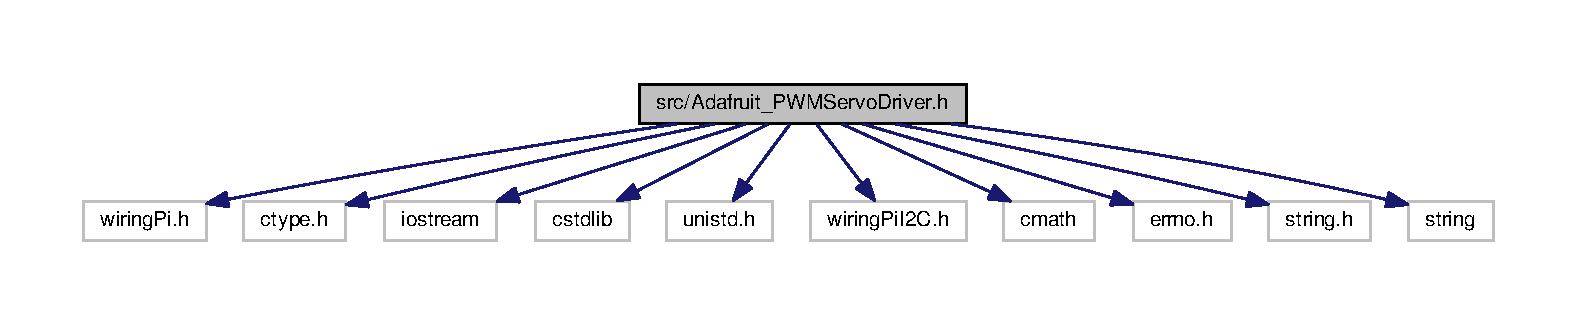
\includegraphics[width=350pt]{Adafruit__PWMServoDriver_8h__incl}
\end{center}
\end{figure}
This graph shows which files directly or indirectly include this file\+:
\nopagebreak
\begin{figure}[H]
\begin{center}
\leavevmode
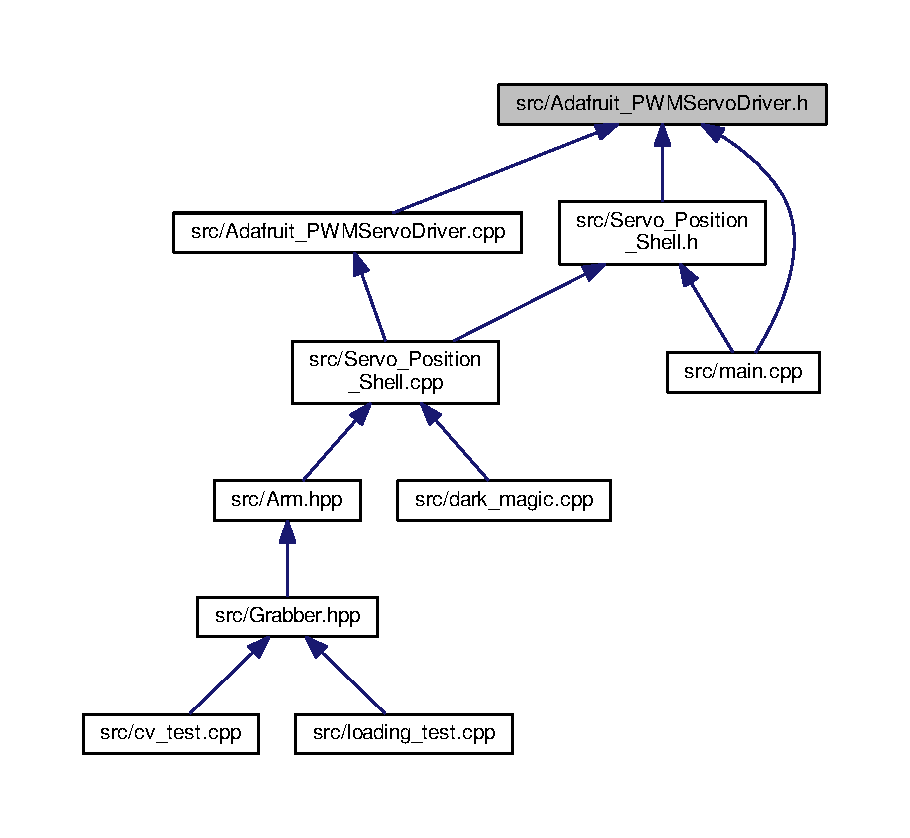
\includegraphics[width=350pt]{Adafruit__PWMServoDriver_8h__dep__incl}
\end{center}
\end{figure}
\subsection*{Classes}
\begin{DoxyCompactItemize}
\item 
class \hyperlink{classAdafruit__PWMServoDriver}{Adafruit\+\_\+\+P\+W\+M\+Servo\+Driver}
\end{DoxyCompactItemize}
\subsection*{Macros}
\begin{DoxyCompactItemize}
\item 
\#define \hyperlink{Adafruit__PWMServoDriver_8h_ad58a880e68f5aa69092c658a86641a8e}{P\+C\+A9685\+\_\+\+S\+U\+B\+A\+D\+R1}~0x2
\item 
\#define \hyperlink{Adafruit__PWMServoDriver_8h_a845ec28ef89ed81642ea5f41691d4b51}{P\+C\+A9685\+\_\+\+S\+U\+B\+A\+D\+R2}~0x3
\item 
\#define \hyperlink{Adafruit__PWMServoDriver_8h_a7f60829a2cf850c02403f5c7193b0f00}{P\+C\+A9685\+\_\+\+S\+U\+B\+A\+D\+R3}~0x4
\item 
\#define \hyperlink{Adafruit__PWMServoDriver_8h_aec642e3f25e7f83072d68acb14ae4e74}{P\+C\+A9685\+\_\+\+M\+O\+D\+E1}~0x0
\item 
\#define \hyperlink{Adafruit__PWMServoDriver_8h_a7175106bbec978d9acc85dc7485235a3}{P\+C\+A9685\+\_\+\+P\+R\+E\+S\+C\+A\+L\+E}~0x\+F\+E
\item 
\#define \hyperlink{Adafruit__PWMServoDriver_8h_a62f7dbcbb1fcf1084804f19a5b42248f}{L\+E\+D0\+\_\+\+O\+N\+\_\+\+L}~0x6
\item 
\#define \hyperlink{Adafruit__PWMServoDriver_8h_a03deab303c78b50c629847b9e0de106b}{L\+E\+D0\+\_\+\+O\+N\+\_\+\+H}~0x7
\item 
\#define \hyperlink{Adafruit__PWMServoDriver_8h_a00e3f4b43121817be365b2f22e8bad84}{L\+E\+D0\+\_\+\+O\+F\+F\+\_\+\+L}~0x8
\item 
\#define \hyperlink{Adafruit__PWMServoDriver_8h_a6d8ff6441f8d2a4fb7b4afd36b8fd329}{L\+E\+D0\+\_\+\+O\+F\+F\+\_\+\+H}~0x9
\item 
\#define \hyperlink{Adafruit__PWMServoDriver_8h_acc163ea7453bc87b5934e8b2bc838556}{A\+L\+L\+L\+E\+D\+\_\+\+O\+N\+\_\+\+L}~0x\+F\+A
\item 
\#define \hyperlink{Adafruit__PWMServoDriver_8h_a470526d36c4db534d04ec1452ddde736}{A\+L\+L\+L\+E\+D\+\_\+\+O\+N\+\_\+\+H}~0x\+F\+B
\item 
\#define \hyperlink{Adafruit__PWMServoDriver_8h_a6dc494d4156968e9cd24f7ac07bf2ee3}{A\+L\+L\+L\+E\+D\+\_\+\+O\+F\+F\+\_\+\+L}~0x\+F\+C
\item 
\#define \hyperlink{Adafruit__PWMServoDriver_8h_a11632001b28c990e5f6dee015e945b1d}{A\+L\+L\+L\+E\+D\+\_\+\+O\+F\+F\+\_\+\+H}~0x\+F\+D
\item 
\#define \hyperlink{Adafruit__PWMServoDriver_8h_ab077fa1127453be2bd9d4c3c8a768fa7}{uint8\+\_\+t}~unsigned char
\item 
\#define \hyperlink{Adafruit__PWMServoDriver_8h_a395b3b2bf5cb4674ab41b6bda68c15bb}{uint16\+\_\+t}~unsigned short int
\end{DoxyCompactItemize}


\subsection{Detailed Description}
\begin{DoxyAuthor}{Author}
Limor Fried/\+Ladyada 

Nickolas Neely  Contains the function and class headers necessary for the P\+W\+M servo driver. 
\end{DoxyAuthor}


Definition in file \hyperlink{Adafruit__PWMServoDriver_8h_source}{Adafruit\+\_\+\+P\+W\+M\+Servo\+Driver.\+h}.



\subsection{Macro Definition Documentation}
\hypertarget{Adafruit__PWMServoDriver_8h_a11632001b28c990e5f6dee015e945b1d}{\index{Adafruit\+\_\+\+P\+W\+M\+Servo\+Driver.\+h@{Adafruit\+\_\+\+P\+W\+M\+Servo\+Driver.\+h}!A\+L\+L\+L\+E\+D\+\_\+\+O\+F\+F\+\_\+\+H@{A\+L\+L\+L\+E\+D\+\_\+\+O\+F\+F\+\_\+\+H}}
\index{A\+L\+L\+L\+E\+D\+\_\+\+O\+F\+F\+\_\+\+H@{A\+L\+L\+L\+E\+D\+\_\+\+O\+F\+F\+\_\+\+H}!Adafruit\+\_\+\+P\+W\+M\+Servo\+Driver.\+h@{Adafruit\+\_\+\+P\+W\+M\+Servo\+Driver.\+h}}
\subsubsection[{A\+L\+L\+L\+E\+D\+\_\+\+O\+F\+F\+\_\+\+H}]{\setlength{\rightskip}{0pt plus 5cm}\#define A\+L\+L\+L\+E\+D\+\_\+\+O\+F\+F\+\_\+\+H~0x\+F\+D}}\label{Adafruit__PWMServoDriver_8h_a11632001b28c990e5f6dee015e945b1d}


Definition at line \hyperlink{Adafruit__PWMServoDriver_8h_source_l00062}{62} of file \hyperlink{Adafruit__PWMServoDriver_8h_source}{Adafruit\+\_\+\+P\+W\+M\+Servo\+Driver.\+h}.

\hypertarget{Adafruit__PWMServoDriver_8h_a6dc494d4156968e9cd24f7ac07bf2ee3}{\index{Adafruit\+\_\+\+P\+W\+M\+Servo\+Driver.\+h@{Adafruit\+\_\+\+P\+W\+M\+Servo\+Driver.\+h}!A\+L\+L\+L\+E\+D\+\_\+\+O\+F\+F\+\_\+\+L@{A\+L\+L\+L\+E\+D\+\_\+\+O\+F\+F\+\_\+\+L}}
\index{A\+L\+L\+L\+E\+D\+\_\+\+O\+F\+F\+\_\+\+L@{A\+L\+L\+L\+E\+D\+\_\+\+O\+F\+F\+\_\+\+L}!Adafruit\+\_\+\+P\+W\+M\+Servo\+Driver.\+h@{Adafruit\+\_\+\+P\+W\+M\+Servo\+Driver.\+h}}
\subsubsection[{A\+L\+L\+L\+E\+D\+\_\+\+O\+F\+F\+\_\+\+L}]{\setlength{\rightskip}{0pt plus 5cm}\#define A\+L\+L\+L\+E\+D\+\_\+\+O\+F\+F\+\_\+\+L~0x\+F\+C}}\label{Adafruit__PWMServoDriver_8h_a6dc494d4156968e9cd24f7ac07bf2ee3}


Definition at line \hyperlink{Adafruit__PWMServoDriver_8h_source_l00061}{61} of file \hyperlink{Adafruit__PWMServoDriver_8h_source}{Adafruit\+\_\+\+P\+W\+M\+Servo\+Driver.\+h}.

\hypertarget{Adafruit__PWMServoDriver_8h_a470526d36c4db534d04ec1452ddde736}{\index{Adafruit\+\_\+\+P\+W\+M\+Servo\+Driver.\+h@{Adafruit\+\_\+\+P\+W\+M\+Servo\+Driver.\+h}!A\+L\+L\+L\+E\+D\+\_\+\+O\+N\+\_\+\+H@{A\+L\+L\+L\+E\+D\+\_\+\+O\+N\+\_\+\+H}}
\index{A\+L\+L\+L\+E\+D\+\_\+\+O\+N\+\_\+\+H@{A\+L\+L\+L\+E\+D\+\_\+\+O\+N\+\_\+\+H}!Adafruit\+\_\+\+P\+W\+M\+Servo\+Driver.\+h@{Adafruit\+\_\+\+P\+W\+M\+Servo\+Driver.\+h}}
\subsubsection[{A\+L\+L\+L\+E\+D\+\_\+\+O\+N\+\_\+\+H}]{\setlength{\rightskip}{0pt plus 5cm}\#define A\+L\+L\+L\+E\+D\+\_\+\+O\+N\+\_\+\+H~0x\+F\+B}}\label{Adafruit__PWMServoDriver_8h_a470526d36c4db534d04ec1452ddde736}


Definition at line \hyperlink{Adafruit__PWMServoDriver_8h_source_l00060}{60} of file \hyperlink{Adafruit__PWMServoDriver_8h_source}{Adafruit\+\_\+\+P\+W\+M\+Servo\+Driver.\+h}.

\hypertarget{Adafruit__PWMServoDriver_8h_acc163ea7453bc87b5934e8b2bc838556}{\index{Adafruit\+\_\+\+P\+W\+M\+Servo\+Driver.\+h@{Adafruit\+\_\+\+P\+W\+M\+Servo\+Driver.\+h}!A\+L\+L\+L\+E\+D\+\_\+\+O\+N\+\_\+\+L@{A\+L\+L\+L\+E\+D\+\_\+\+O\+N\+\_\+\+L}}
\index{A\+L\+L\+L\+E\+D\+\_\+\+O\+N\+\_\+\+L@{A\+L\+L\+L\+E\+D\+\_\+\+O\+N\+\_\+\+L}!Adafruit\+\_\+\+P\+W\+M\+Servo\+Driver.\+h@{Adafruit\+\_\+\+P\+W\+M\+Servo\+Driver.\+h}}
\subsubsection[{A\+L\+L\+L\+E\+D\+\_\+\+O\+N\+\_\+\+L}]{\setlength{\rightskip}{0pt plus 5cm}\#define A\+L\+L\+L\+E\+D\+\_\+\+O\+N\+\_\+\+L~0x\+F\+A}}\label{Adafruit__PWMServoDriver_8h_acc163ea7453bc87b5934e8b2bc838556}


Definition at line \hyperlink{Adafruit__PWMServoDriver_8h_source_l00059}{59} of file \hyperlink{Adafruit__PWMServoDriver_8h_source}{Adafruit\+\_\+\+P\+W\+M\+Servo\+Driver.\+h}.

\hypertarget{Adafruit__PWMServoDriver_8h_a6d8ff6441f8d2a4fb7b4afd36b8fd329}{\index{Adafruit\+\_\+\+P\+W\+M\+Servo\+Driver.\+h@{Adafruit\+\_\+\+P\+W\+M\+Servo\+Driver.\+h}!L\+E\+D0\+\_\+\+O\+F\+F\+\_\+\+H@{L\+E\+D0\+\_\+\+O\+F\+F\+\_\+\+H}}
\index{L\+E\+D0\+\_\+\+O\+F\+F\+\_\+\+H@{L\+E\+D0\+\_\+\+O\+F\+F\+\_\+\+H}!Adafruit\+\_\+\+P\+W\+M\+Servo\+Driver.\+h@{Adafruit\+\_\+\+P\+W\+M\+Servo\+Driver.\+h}}
\subsubsection[{L\+E\+D0\+\_\+\+O\+F\+F\+\_\+\+H}]{\setlength{\rightskip}{0pt plus 5cm}\#define L\+E\+D0\+\_\+\+O\+F\+F\+\_\+\+H~0x9}}\label{Adafruit__PWMServoDriver_8h_a6d8ff6441f8d2a4fb7b4afd36b8fd329}


Definition at line \hyperlink{Adafruit__PWMServoDriver_8h_source_l00057}{57} of file \hyperlink{Adafruit__PWMServoDriver_8h_source}{Adafruit\+\_\+\+P\+W\+M\+Servo\+Driver.\+h}.

\hypertarget{Adafruit__PWMServoDriver_8h_a00e3f4b43121817be365b2f22e8bad84}{\index{Adafruit\+\_\+\+P\+W\+M\+Servo\+Driver.\+h@{Adafruit\+\_\+\+P\+W\+M\+Servo\+Driver.\+h}!L\+E\+D0\+\_\+\+O\+F\+F\+\_\+\+L@{L\+E\+D0\+\_\+\+O\+F\+F\+\_\+\+L}}
\index{L\+E\+D0\+\_\+\+O\+F\+F\+\_\+\+L@{L\+E\+D0\+\_\+\+O\+F\+F\+\_\+\+L}!Adafruit\+\_\+\+P\+W\+M\+Servo\+Driver.\+h@{Adafruit\+\_\+\+P\+W\+M\+Servo\+Driver.\+h}}
\subsubsection[{L\+E\+D0\+\_\+\+O\+F\+F\+\_\+\+L}]{\setlength{\rightskip}{0pt plus 5cm}\#define L\+E\+D0\+\_\+\+O\+F\+F\+\_\+\+L~0x8}}\label{Adafruit__PWMServoDriver_8h_a00e3f4b43121817be365b2f22e8bad84}


Definition at line \hyperlink{Adafruit__PWMServoDriver_8h_source_l00056}{56} of file \hyperlink{Adafruit__PWMServoDriver_8h_source}{Adafruit\+\_\+\+P\+W\+M\+Servo\+Driver.\+h}.

\hypertarget{Adafruit__PWMServoDriver_8h_a03deab303c78b50c629847b9e0de106b}{\index{Adafruit\+\_\+\+P\+W\+M\+Servo\+Driver.\+h@{Adafruit\+\_\+\+P\+W\+M\+Servo\+Driver.\+h}!L\+E\+D0\+\_\+\+O\+N\+\_\+\+H@{L\+E\+D0\+\_\+\+O\+N\+\_\+\+H}}
\index{L\+E\+D0\+\_\+\+O\+N\+\_\+\+H@{L\+E\+D0\+\_\+\+O\+N\+\_\+\+H}!Adafruit\+\_\+\+P\+W\+M\+Servo\+Driver.\+h@{Adafruit\+\_\+\+P\+W\+M\+Servo\+Driver.\+h}}
\subsubsection[{L\+E\+D0\+\_\+\+O\+N\+\_\+\+H}]{\setlength{\rightskip}{0pt plus 5cm}\#define L\+E\+D0\+\_\+\+O\+N\+\_\+\+H~0x7}}\label{Adafruit__PWMServoDriver_8h_a03deab303c78b50c629847b9e0de106b}


Definition at line \hyperlink{Adafruit__PWMServoDriver_8h_source_l00055}{55} of file \hyperlink{Adafruit__PWMServoDriver_8h_source}{Adafruit\+\_\+\+P\+W\+M\+Servo\+Driver.\+h}.

\hypertarget{Adafruit__PWMServoDriver_8h_a62f7dbcbb1fcf1084804f19a5b42248f}{\index{Adafruit\+\_\+\+P\+W\+M\+Servo\+Driver.\+h@{Adafruit\+\_\+\+P\+W\+M\+Servo\+Driver.\+h}!L\+E\+D0\+\_\+\+O\+N\+\_\+\+L@{L\+E\+D0\+\_\+\+O\+N\+\_\+\+L}}
\index{L\+E\+D0\+\_\+\+O\+N\+\_\+\+L@{L\+E\+D0\+\_\+\+O\+N\+\_\+\+L}!Adafruit\+\_\+\+P\+W\+M\+Servo\+Driver.\+h@{Adafruit\+\_\+\+P\+W\+M\+Servo\+Driver.\+h}}
\subsubsection[{L\+E\+D0\+\_\+\+O\+N\+\_\+\+L}]{\setlength{\rightskip}{0pt plus 5cm}\#define L\+E\+D0\+\_\+\+O\+N\+\_\+\+L~0x6}}\label{Adafruit__PWMServoDriver_8h_a62f7dbcbb1fcf1084804f19a5b42248f}


Definition at line \hyperlink{Adafruit__PWMServoDriver_8h_source_l00054}{54} of file \hyperlink{Adafruit__PWMServoDriver_8h_source}{Adafruit\+\_\+\+P\+W\+M\+Servo\+Driver.\+h}.

\hypertarget{Adafruit__PWMServoDriver_8h_aec642e3f25e7f83072d68acb14ae4e74}{\index{Adafruit\+\_\+\+P\+W\+M\+Servo\+Driver.\+h@{Adafruit\+\_\+\+P\+W\+M\+Servo\+Driver.\+h}!P\+C\+A9685\+\_\+\+M\+O\+D\+E1@{P\+C\+A9685\+\_\+\+M\+O\+D\+E1}}
\index{P\+C\+A9685\+\_\+\+M\+O\+D\+E1@{P\+C\+A9685\+\_\+\+M\+O\+D\+E1}!Adafruit\+\_\+\+P\+W\+M\+Servo\+Driver.\+h@{Adafruit\+\_\+\+P\+W\+M\+Servo\+Driver.\+h}}
\subsubsection[{P\+C\+A9685\+\_\+\+M\+O\+D\+E1}]{\setlength{\rightskip}{0pt plus 5cm}\#define P\+C\+A9685\+\_\+\+M\+O\+D\+E1~0x0}}\label{Adafruit__PWMServoDriver_8h_aec642e3f25e7f83072d68acb14ae4e74}


Definition at line \hyperlink{Adafruit__PWMServoDriver_8h_source_l00051}{51} of file \hyperlink{Adafruit__PWMServoDriver_8h_source}{Adafruit\+\_\+\+P\+W\+M\+Servo\+Driver.\+h}.

\hypertarget{Adafruit__PWMServoDriver_8h_a7175106bbec978d9acc85dc7485235a3}{\index{Adafruit\+\_\+\+P\+W\+M\+Servo\+Driver.\+h@{Adafruit\+\_\+\+P\+W\+M\+Servo\+Driver.\+h}!P\+C\+A9685\+\_\+\+P\+R\+E\+S\+C\+A\+L\+E@{P\+C\+A9685\+\_\+\+P\+R\+E\+S\+C\+A\+L\+E}}
\index{P\+C\+A9685\+\_\+\+P\+R\+E\+S\+C\+A\+L\+E@{P\+C\+A9685\+\_\+\+P\+R\+E\+S\+C\+A\+L\+E}!Adafruit\+\_\+\+P\+W\+M\+Servo\+Driver.\+h@{Adafruit\+\_\+\+P\+W\+M\+Servo\+Driver.\+h}}
\subsubsection[{P\+C\+A9685\+\_\+\+P\+R\+E\+S\+C\+A\+L\+E}]{\setlength{\rightskip}{0pt plus 5cm}\#define P\+C\+A9685\+\_\+\+P\+R\+E\+S\+C\+A\+L\+E~0x\+F\+E}}\label{Adafruit__PWMServoDriver_8h_a7175106bbec978d9acc85dc7485235a3}


Definition at line \hyperlink{Adafruit__PWMServoDriver_8h_source_l00052}{52} of file \hyperlink{Adafruit__PWMServoDriver_8h_source}{Adafruit\+\_\+\+P\+W\+M\+Servo\+Driver.\+h}.

\hypertarget{Adafruit__PWMServoDriver_8h_ad58a880e68f5aa69092c658a86641a8e}{\index{Adafruit\+\_\+\+P\+W\+M\+Servo\+Driver.\+h@{Adafruit\+\_\+\+P\+W\+M\+Servo\+Driver.\+h}!P\+C\+A9685\+\_\+\+S\+U\+B\+A\+D\+R1@{P\+C\+A9685\+\_\+\+S\+U\+B\+A\+D\+R1}}
\index{P\+C\+A9685\+\_\+\+S\+U\+B\+A\+D\+R1@{P\+C\+A9685\+\_\+\+S\+U\+B\+A\+D\+R1}!Adafruit\+\_\+\+P\+W\+M\+Servo\+Driver.\+h@{Adafruit\+\_\+\+P\+W\+M\+Servo\+Driver.\+h}}
\subsubsection[{P\+C\+A9685\+\_\+\+S\+U\+B\+A\+D\+R1}]{\setlength{\rightskip}{0pt plus 5cm}\#define P\+C\+A9685\+\_\+\+S\+U\+B\+A\+D\+R1~0x2}}\label{Adafruit__PWMServoDriver_8h_ad58a880e68f5aa69092c658a86641a8e}


Definition at line \hyperlink{Adafruit__PWMServoDriver_8h_source_l00047}{47} of file \hyperlink{Adafruit__PWMServoDriver_8h_source}{Adafruit\+\_\+\+P\+W\+M\+Servo\+Driver.\+h}.

\hypertarget{Adafruit__PWMServoDriver_8h_a845ec28ef89ed81642ea5f41691d4b51}{\index{Adafruit\+\_\+\+P\+W\+M\+Servo\+Driver.\+h@{Adafruit\+\_\+\+P\+W\+M\+Servo\+Driver.\+h}!P\+C\+A9685\+\_\+\+S\+U\+B\+A\+D\+R2@{P\+C\+A9685\+\_\+\+S\+U\+B\+A\+D\+R2}}
\index{P\+C\+A9685\+\_\+\+S\+U\+B\+A\+D\+R2@{P\+C\+A9685\+\_\+\+S\+U\+B\+A\+D\+R2}!Adafruit\+\_\+\+P\+W\+M\+Servo\+Driver.\+h@{Adafruit\+\_\+\+P\+W\+M\+Servo\+Driver.\+h}}
\subsubsection[{P\+C\+A9685\+\_\+\+S\+U\+B\+A\+D\+R2}]{\setlength{\rightskip}{0pt plus 5cm}\#define P\+C\+A9685\+\_\+\+S\+U\+B\+A\+D\+R2~0x3}}\label{Adafruit__PWMServoDriver_8h_a845ec28ef89ed81642ea5f41691d4b51}


Definition at line \hyperlink{Adafruit__PWMServoDriver_8h_source_l00048}{48} of file \hyperlink{Adafruit__PWMServoDriver_8h_source}{Adafruit\+\_\+\+P\+W\+M\+Servo\+Driver.\+h}.

\hypertarget{Adafruit__PWMServoDriver_8h_a7f60829a2cf850c02403f5c7193b0f00}{\index{Adafruit\+\_\+\+P\+W\+M\+Servo\+Driver.\+h@{Adafruit\+\_\+\+P\+W\+M\+Servo\+Driver.\+h}!P\+C\+A9685\+\_\+\+S\+U\+B\+A\+D\+R3@{P\+C\+A9685\+\_\+\+S\+U\+B\+A\+D\+R3}}
\index{P\+C\+A9685\+\_\+\+S\+U\+B\+A\+D\+R3@{P\+C\+A9685\+\_\+\+S\+U\+B\+A\+D\+R3}!Adafruit\+\_\+\+P\+W\+M\+Servo\+Driver.\+h@{Adafruit\+\_\+\+P\+W\+M\+Servo\+Driver.\+h}}
\subsubsection[{P\+C\+A9685\+\_\+\+S\+U\+B\+A\+D\+R3}]{\setlength{\rightskip}{0pt plus 5cm}\#define P\+C\+A9685\+\_\+\+S\+U\+B\+A\+D\+R3~0x4}}\label{Adafruit__PWMServoDriver_8h_a7f60829a2cf850c02403f5c7193b0f00}


Definition at line \hyperlink{Adafruit__PWMServoDriver_8h_source_l00049}{49} of file \hyperlink{Adafruit__PWMServoDriver_8h_source}{Adafruit\+\_\+\+P\+W\+M\+Servo\+Driver.\+h}.

\hypertarget{Adafruit__PWMServoDriver_8h_a395b3b2bf5cb4674ab41b6bda68c15bb}{\index{Adafruit\+\_\+\+P\+W\+M\+Servo\+Driver.\+h@{Adafruit\+\_\+\+P\+W\+M\+Servo\+Driver.\+h}!uint16\+\_\+t@{uint16\+\_\+t}}
\index{uint16\+\_\+t@{uint16\+\_\+t}!Adafruit\+\_\+\+P\+W\+M\+Servo\+Driver.\+h@{Adafruit\+\_\+\+P\+W\+M\+Servo\+Driver.\+h}}
\subsubsection[{uint16\+\_\+t}]{\setlength{\rightskip}{0pt plus 5cm}\#define uint16\+\_\+t~unsigned short int}}\label{Adafruit__PWMServoDriver_8h_a395b3b2bf5cb4674ab41b6bda68c15bb}


Definition at line \hyperlink{Adafruit__PWMServoDriver_8h_source_l00069}{69} of file \hyperlink{Adafruit__PWMServoDriver_8h_source}{Adafruit\+\_\+\+P\+W\+M\+Servo\+Driver.\+h}.

\hypertarget{Adafruit__PWMServoDriver_8h_ab077fa1127453be2bd9d4c3c8a768fa7}{\index{Adafruit\+\_\+\+P\+W\+M\+Servo\+Driver.\+h@{Adafruit\+\_\+\+P\+W\+M\+Servo\+Driver.\+h}!uint8\+\_\+t@{uint8\+\_\+t}}
\index{uint8\+\_\+t@{uint8\+\_\+t}!Adafruit\+\_\+\+P\+W\+M\+Servo\+Driver.\+h@{Adafruit\+\_\+\+P\+W\+M\+Servo\+Driver.\+h}}
\subsubsection[{uint8\+\_\+t}]{\setlength{\rightskip}{0pt plus 5cm}\#define uint8\+\_\+t~unsigned char}}\label{Adafruit__PWMServoDriver_8h_ab077fa1127453be2bd9d4c3c8a768fa7}


Definition at line \hyperlink{Adafruit__PWMServoDriver_8h_source_l00065}{65} of file \hyperlink{Adafruit__PWMServoDriver_8h_source}{Adafruit\+\_\+\+P\+W\+M\+Servo\+Driver.\+h}.


\hypertarget{Adafruit__PWMServoDriver_8h_source}{\section{Adafruit\+\_\+\+P\+W\+M\+Servo\+Driver.\+h}
\label{Adafruit__PWMServoDriver_8h_source}\index{src/\+Adafruit\+\_\+\+P\+W\+M\+Servo\+Driver.\+h@{src/\+Adafruit\+\_\+\+P\+W\+M\+Servo\+Driver.\+h}}
}

\begin{DoxyCode}
00001 
00009 \textcolor{comment}{/* File: Adafruit\_PWMServoDriver.h}
00010 \textcolor{comment}{ * Credit to Limor Fried/Ladyada for PWM servo driver code. }
00011 \textcolor{comment}{ * Editted by: Nickolas Neely for ChipChipArray Raspberry Pi }
00012 \textcolor{comment}{ */}
00013 
00014 \textcolor{comment}{/*************************************************** }
00015 \textcolor{comment}{  This is a library for our Adafruit 16-channel PWM & Servo driver}
00016 \textcolor{comment}{}
00017 \textcolor{comment}{  Pick one up today in the adafruit shop!}
00018 \textcolor{comment}{  ------> http://www.adafruit.com/products/815}
00019 \textcolor{comment}{}
00020 \textcolor{comment}{  These displays use I2C to communicate, 2 pins are required to  }
00021 \textcolor{comment}{  interface. For Arduino UNOs, thats SCL -> Analog 5, SDA -> Analog 4}
00022 \textcolor{comment}{}
00023 \textcolor{comment}{  Adafruit invests time and resources providing this open source code, }
00024 \textcolor{comment}{  please support Adafruit and open-source hardware by purchasing }
00025 \textcolor{comment}{  products from Adafruit!}
00026 \textcolor{comment}{}
00027 \textcolor{comment}{  Written by Limor Fried/Ladyada for Adafruit Industries.  }
00028 \textcolor{comment}{  BSD license, all text above must be included in any redistribution}
00029 \textcolor{comment}{ ****************************************************/}
00030 
00031 \textcolor{preprocessor}{#ifndef \_ADAFRUIT\_PWMServoDriver\_H}
00032 \textcolor{preprocessor}{#define \_ADAFRUIT\_PWMServoDriver\_H}
00033 
00034 \textcolor{preprocessor}{#include <wiringPi.h>}
00035 \textcolor{preprocessor}{#include <ctype.h>}
00036 \textcolor{preprocessor}{#include <iostream>}
00037 \textcolor{preprocessor}{#include <cstdlib>}
00038 \textcolor{preprocessor}{#include <unistd.h>}
00039 \textcolor{preprocessor}{#include <wiringPiI2C.h>}
00040 \textcolor{preprocessor}{#include <cmath>}
00041 \textcolor{preprocessor}{#include <errno.h>}
00042 \textcolor{preprocessor}{#include <string.h>}
00043 \textcolor{preprocessor}{#include <string>}
00044 
00045 \textcolor{keyword}{using namespace }\hyperlink{namespacestd}{std};
00046 
\hypertarget{Adafruit__PWMServoDriver_8h_source_l00047}{}\hyperlink{Adafruit__PWMServoDriver_8h_ad58a880e68f5aa69092c658a86641a8e}{00047} \textcolor{preprocessor}{#define PCA9685\_SUBADR1 0x2}
\hypertarget{Adafruit__PWMServoDriver_8h_source_l00048}{}\hyperlink{Adafruit__PWMServoDriver_8h_a845ec28ef89ed81642ea5f41691d4b51}{00048} \textcolor{preprocessor}{#define PCA9685\_SUBADR2 0x3}
\hypertarget{Adafruit__PWMServoDriver_8h_source_l00049}{}\hyperlink{Adafruit__PWMServoDriver_8h_a7f60829a2cf850c02403f5c7193b0f00}{00049} \textcolor{preprocessor}{#define PCA9685\_SUBADR3 0x4}
00050 
\hypertarget{Adafruit__PWMServoDriver_8h_source_l00051}{}\hyperlink{Adafruit__PWMServoDriver_8h_aec642e3f25e7f83072d68acb14ae4e74}{00051} \textcolor{preprocessor}{#define PCA9685\_MODE1 0x0}
\hypertarget{Adafruit__PWMServoDriver_8h_source_l00052}{}\hyperlink{Adafruit__PWMServoDriver_8h_a7175106bbec978d9acc85dc7485235a3}{00052} \textcolor{preprocessor}{#define PCA9685\_PRESCALE 0xFE}
00053 
\hypertarget{Adafruit__PWMServoDriver_8h_source_l00054}{}\hyperlink{Adafruit__PWMServoDriver_8h_a62f7dbcbb1fcf1084804f19a5b42248f}{00054} \textcolor{preprocessor}{#define LED0\_ON\_L 0x6}
\hypertarget{Adafruit__PWMServoDriver_8h_source_l00055}{}\hyperlink{Adafruit__PWMServoDriver_8h_a03deab303c78b50c629847b9e0de106b}{00055} \textcolor{preprocessor}{#define LED0\_ON\_H 0x7}
\hypertarget{Adafruit__PWMServoDriver_8h_source_l00056}{}\hyperlink{Adafruit__PWMServoDriver_8h_a00e3f4b43121817be365b2f22e8bad84}{00056} \textcolor{preprocessor}{#define LED0\_OFF\_L 0x8}
\hypertarget{Adafruit__PWMServoDriver_8h_source_l00057}{}\hyperlink{Adafruit__PWMServoDriver_8h_a6d8ff6441f8d2a4fb7b4afd36b8fd329}{00057} \textcolor{preprocessor}{#define LED0\_OFF\_H 0x9}
00058 
\hypertarget{Adafruit__PWMServoDriver_8h_source_l00059}{}\hyperlink{Adafruit__PWMServoDriver_8h_acc163ea7453bc87b5934e8b2bc838556}{00059} \textcolor{preprocessor}{#define ALLLED\_ON\_L 0xFA}
\hypertarget{Adafruit__PWMServoDriver_8h_source_l00060}{}\hyperlink{Adafruit__PWMServoDriver_8h_a470526d36c4db534d04ec1452ddde736}{00060} \textcolor{preprocessor}{#define ALLLED\_ON\_H 0xFB}
\hypertarget{Adafruit__PWMServoDriver_8h_source_l00061}{}\hyperlink{Adafruit__PWMServoDriver_8h_a6dc494d4156968e9cd24f7ac07bf2ee3}{00061} \textcolor{preprocessor}{#define ALLLED\_OFF\_L 0xFC}
\hypertarget{Adafruit__PWMServoDriver_8h_source_l00062}{}\hyperlink{Adafruit__PWMServoDriver_8h_a11632001b28c990e5f6dee015e945b1d}{00062} \textcolor{preprocessor}{#define ALLLED\_OFF\_H 0xFD}
00063 
00064 \textcolor{preprocessor}{#ifndef uint8\_t}
\hypertarget{Adafruit__PWMServoDriver_8h_source_l00065}{}\hyperlink{Adafruit__PWMServoDriver_8h_ab077fa1127453be2bd9d4c3c8a768fa7}{00065} \textcolor{preprocessor}{#define uint8\_t unsigned char}
00066 \textcolor{preprocessor}{#endif}
00067 
00068 \textcolor{preprocessor}{#ifndef uint16\_t}
\hypertarget{Adafruit__PWMServoDriver_8h_source_l00069}{}\hyperlink{Adafruit__PWMServoDriver_8h_a395b3b2bf5cb4674ab41b6bda68c15bb}{00069} \textcolor{preprocessor}{#define uint16\_t unsigned short int}
00070 \textcolor{preprocessor}{#endif}
00071 
00072 
\hypertarget{Adafruit__PWMServoDriver_8h_source_l00073}{}\hyperlink{classAdafruit__PWMServoDriver}{00073} \textcolor{keyword}{class }\hyperlink{classAdafruit__PWMServoDriver}{Adafruit\_PWMServoDriver} \{
00074  \textcolor{keyword}{public}:
00075   \hyperlink{classAdafruit__PWMServoDriver}{Adafruit\_PWMServoDriver}(\hyperlink{Adafruit__PWMServoDriver_8h_ab077fa1127453be2bd9d4c3c8a768fa7}{uint8\_t} addr = 0x41);
00076   \textcolor{keywordtype}{void} begin(\textcolor{keywordtype}{void});
00077   \textcolor{keywordtype}{void} reset(\textcolor{keywordtype}{void});
00078   \textcolor{keywordtype}{void} setPWMFreq(\textcolor{keywordtype}{float} freq);
00079   \textcolor{keywordtype}{void} setPWM(\hyperlink{Adafruit__PWMServoDriver_8h_ab077fa1127453be2bd9d4c3c8a768fa7}{uint8\_t} num, \hyperlink{Adafruit__PWMServoDriver_8h_a395b3b2bf5cb4674ab41b6bda68c15bb}{uint16\_t} on, \hyperlink{Adafruit__PWMServoDriver_8h_a395b3b2bf5cb4674ab41b6bda68c15bb}{uint16\_t} off);
00080   \textcolor{keywordtype}{void} setPin(\hyperlink{Adafruit__PWMServoDriver_8h_ab077fa1127453be2bd9d4c3c8a768fa7}{uint8\_t} num, \hyperlink{Adafruit__PWMServoDriver_8h_a395b3b2bf5cb4674ab41b6bda68c15bb}{uint16\_t} val, \textcolor{keywordtype}{bool} invert=\textcolor{keyword}{false});
00081 
00082  \textcolor{keyword}{private}:
00083   \hyperlink{Adafruit__PWMServoDriver_8h_ab077fa1127453be2bd9d4c3c8a768fa7}{uint8\_t} \_i2caddr;
00084   \textcolor{keywordtype}{int} \_i2cFD;
00085 
00086   \hyperlink{Adafruit__PWMServoDriver_8h_ab077fa1127453be2bd9d4c3c8a768fa7}{uint8\_t} read8(\hyperlink{Adafruit__PWMServoDriver_8h_ab077fa1127453be2bd9d4c3c8a768fa7}{uint8\_t} addr);
00087   \textcolor{keywordtype}{void} write8(\hyperlink{Adafruit__PWMServoDriver_8h_ab077fa1127453be2bd9d4c3c8a768fa7}{uint8\_t} addr, \hyperlink{Adafruit__PWMServoDriver_8h_ab077fa1127453be2bd9d4c3c8a768fa7}{uint8\_t} d);
00088 \};
00089 
00090 \textcolor{preprocessor}{#endif}
\end{DoxyCode}

\hypertarget{Arm_8hpp}{\section{src/\+Arm.hpp File Reference}
\label{Arm_8hpp}\index{src/\+Arm.\+hpp@{src/\+Arm.\+hpp}}
}


contains the Arm class used to control the robotic arm  


{\ttfamily \#include \char`\"{}definitions.\+hpp\char`\"{}}\\*
{\ttfamily \#include \char`\"{}Servo\+\_\+\+Position\+\_\+\+Shell.\+cpp\char`\"{}}\\*
Include dependency graph for Arm.\+hpp\+:
\nopagebreak
\begin{figure}[H]
\begin{center}
\leavevmode
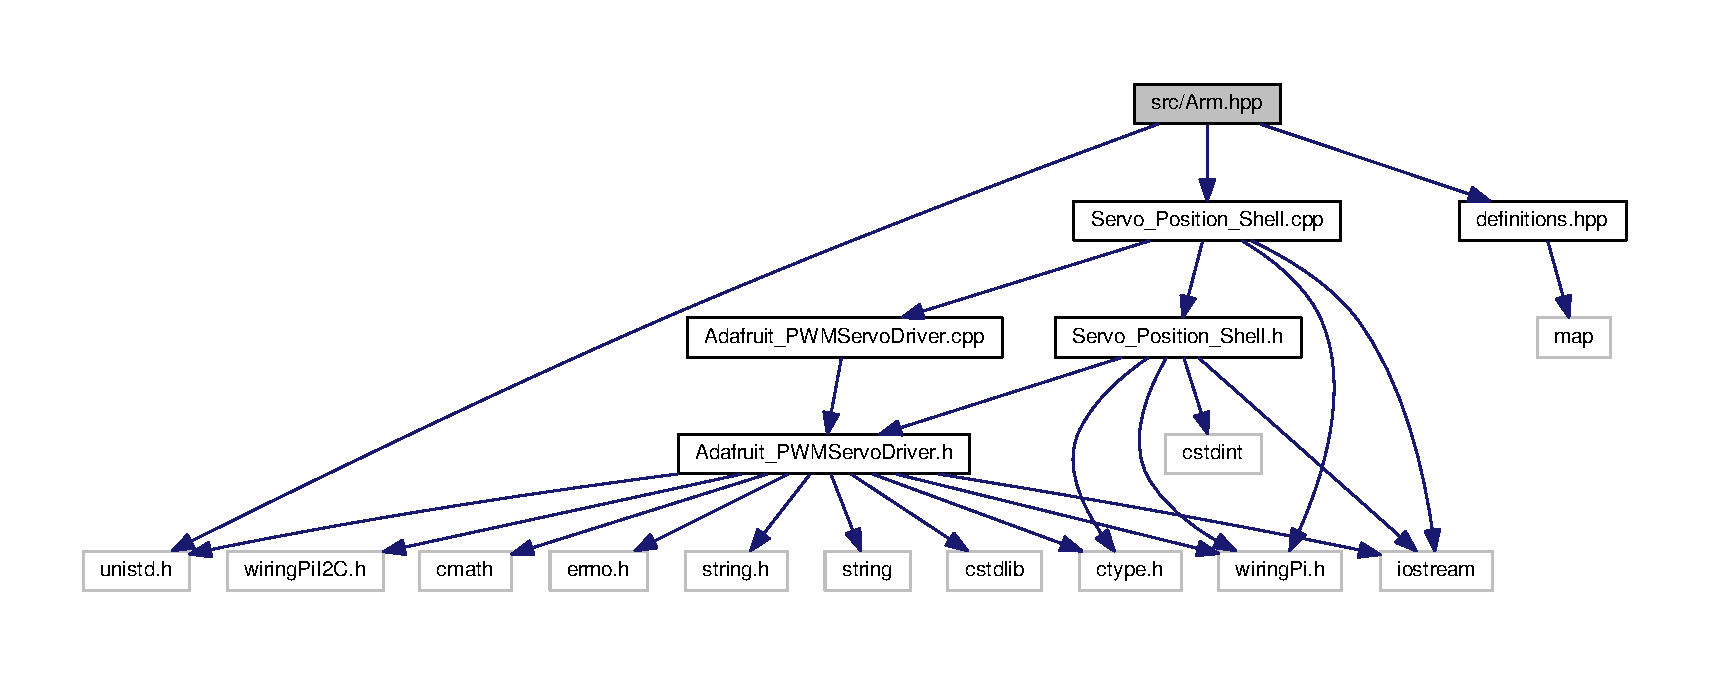
\includegraphics[width=350pt]{Arm_8hpp__incl}
\end{center}
\end{figure}
This graph shows which files directly or indirectly include this file\+:
\nopagebreak
\begin{figure}[H]
\begin{center}
\leavevmode
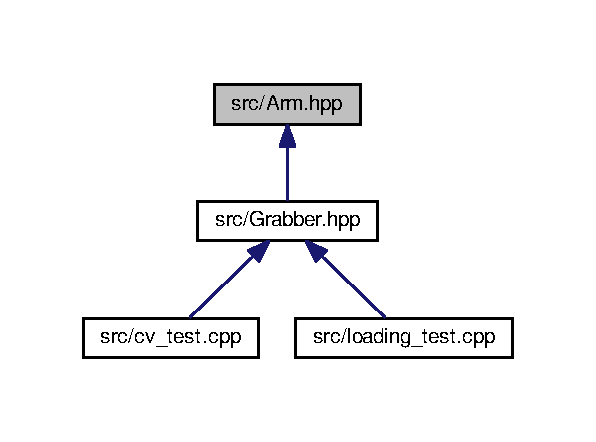
\includegraphics[width=286pt]{Arm_8hpp__dep__incl}
\end{center}
\end{figure}
\subsection*{Classes}
\begin{DoxyCompactItemize}
\item 
class \hyperlink{classChipChipArray_1_1Arm}{Chip\+Chip\+Array\+::\+Arm}
\end{DoxyCompactItemize}
\subsection*{Namespaces}
\begin{DoxyCompactItemize}
\item 
 \hyperlink{namespaceChipChipArray}{Chip\+Chip\+Array}
\begin{DoxyCompactList}\small\item\em contains \hyperlink{classChipChipArray_1_1Block}{Block} class \end{DoxyCompactList}\end{DoxyCompactItemize}


\subsection{Detailed Description}
contains the Arm class used to control the robotic arm 

\begin{DoxyAuthor}{Author}
Samuel Andrew Wisner, \href{mailto:awisner94@gmail.com}{\tt awisner94@gmail.\+com} 
\end{DoxyAuthor}


Definition in file \hyperlink{Arm_8hpp_source}{Arm.\+hpp}.


\hypertarget{Arm_8hpp_source}{\section{Arm.\+hpp}
\label{Arm_8hpp_source}\index{src/\+Arm.\+hpp@{src/\+Arm.\+hpp}}
}

\begin{DoxyCode}
00001 
00007 \textcolor{preprocessor}{#ifndef Arm\_H}
00008 \textcolor{preprocessor}{#define Arm\_H}
00009 
00010 \textcolor{preprocessor}{#include <unistd.h>}
00011 
00012 \textcolor{preprocessor}{#include "\hyperlink{definitions_8hpp}{definitions.hpp}"}
00013 \textcolor{preprocessor}{#include "\hyperlink{Servo__Position__Shell_8cpp}{Servo\_Position\_Shell.cpp}"}
00014 
\hypertarget{Arm_8hpp_source_l00015}{}\hyperlink{Arm_8hpp_a02a3a5fbd2fb97badde7f301b7499e05}{00015} \textcolor{preprocessor}{#define WRIST\_TWIST WRIST\_PAN}
00016 
\hypertarget{Arm_8hpp_source_l00017}{}\hyperlink{namespaceChipChipArray}{00017} \textcolor{keyword}{namespace }\hyperlink{namespaceChipChipArray}{ChipChipArray} \{
\hypertarget{Arm_8hpp_source_l00023}{}\hyperlink{classChipChipArray_1_1Arm}{00023}     \textcolor{keyword}{class }\hyperlink{classChipChipArray_1_1Arm}{Arm} \{
00024         \textcolor{keyword}{public}:
00029             \hyperlink{classChipChipArray_1_1Arm_aeda43d8461e50eaca9aa891ee2863c05}{Arm}();
00030 
\hypertarget{Arm_8hpp_source_l00034}{}\hyperlink{classChipChipArray_1_1Arm_a9ddcea9544b6e2a4315b9dd705df8fdd}{00034}             \hyperlink{definitions_8hpp_adde6aaee8457bee49c2a92621fe22b79}{uint8} \hyperlink{classChipChipArray_1_1Arm_a9ddcea9544b6e2a4315b9dd705df8fdd}{servoPos}[7] = \{ 0, 0, 0, 0, 0, 0, 0 \};
00035 
00041             \textcolor{keywordtype}{void} \hyperlink{classChipChipArray_1_1Arm_a8b077a3791d9fc5ef285c1520fe4c5d8}{BaseTilt}(\hyperlink{definitions_8hpp_adde6aaee8457bee49c2a92621fe22b79}{uint8} a);
00042 
00048             \textcolor{keywordtype}{void} \hyperlink{classChipChipArray_1_1Arm_addaedfe85ff2b14ff00c344fc4b40cd6}{BaseTurn}(\hyperlink{definitions_8hpp_adde6aaee8457bee49c2a92621fe22b79}{uint8} a);
00049 
00053             \textcolor{keywordtype}{void} \hyperlink{classChipChipArray_1_1Arm_abb33b5bb11034554d632f8c9b95b2c44}{ClawOpen}();
00054 
00060             \textcolor{keywordtype}{void} \hyperlink{classChipChipArray_1_1Arm_a20c6fe3fe79c16f492a8c18b91427080}{ClawClose}();
00061 
00068             \textcolor{keywordtype}{void} \hyperlink{classChipChipArray_1_1Arm_af84b91c664baec0f2882dcf4089ae027}{dBaseTilt}(\hyperlink{definitions_8hpp_a74df79fde3c518e55b29ce6360a9c76e}{sint16} a);
00069 
00076             \textcolor{keywordtype}{void} \hyperlink{classChipChipArray_1_1Arm_a980f5bd278cbe06aa21754fb8e0324b3}{dBaseTurn}(\hyperlink{definitions_8hpp_a74df79fde3c518e55b29ce6360a9c76e}{sint16} a);
00077 
00084             \textcolor{keywordtype}{void} \hyperlink{classChipChipArray_1_1Arm_ae8d0a664dd1a0e556cf40c0984035163}{dElbow}(\hyperlink{definitions_8hpp_a74df79fde3c518e55b29ce6360a9c76e}{sint16} a);
00085 
00092             \textcolor{keywordtype}{void} \hyperlink{classChipChipArray_1_1Arm_a43daba698f13a522887ad022b78557bb}{dWristTilt}(\hyperlink{definitions_8hpp_a74df79fde3c518e55b29ce6360a9c76e}{sint16} a);
00093 
00100             \textcolor{keywordtype}{void} \hyperlink{classChipChipArray_1_1Arm_a6bde822b1be63926e21222f36aad67b3}{dWristTwist}(\hyperlink{definitions_8hpp_a74df79fde3c518e55b29ce6360a9c76e}{sint16} a);
00101 
00107             \textcolor{keywordtype}{void} \hyperlink{classChipChipArray_1_1Arm_ac45149e03abfac230b75156bb42e8417}{Elbow}(\hyperlink{definitions_8hpp_adde6aaee8457bee49c2a92621fe22b79}{uint8} a);
00108 
00115             \textcolor{keywordtype}{void} \hyperlink{classChipChipArray_1_1Arm_a8871580fd6a75fd60d99300f2b5c21d1}{Hover}(\hyperlink{definitions_8hpp_adbd1e7a33d3e1751c7b2aa2562d0ecb9}{Zone} zone);
00116 
00122             \textcolor{keywordtype}{void} \hyperlink{classChipChipArray_1_1Arm_ad61f7c1e63eb09981b6c304bd924e217}{WristTilt}(\hyperlink{definitions_8hpp_adde6aaee8457bee49c2a92621fe22b79}{uint8} a);
00123 
00129             \textcolor{keywordtype}{void} \hyperlink{classChipChipArray_1_1Arm_a35ec7756840d9d32dcfbb88d831f087f}{WristTwist}(\hyperlink{definitions_8hpp_adde6aaee8457bee49c2a92621fe22b79}{uint8} a);
00130 
00131         \textcolor{keyword}{protected}:
00132 
00139             \textcolor{keywordtype}{void} \hyperlink{classChipChipArray_1_1Arm_a6da0950c7e3bd4a31264e562916c032d}{dLeftGripper}(\hyperlink{definitions_8hpp_a74df79fde3c518e55b29ce6360a9c76e}{sint16} a);
00140 
00147             \textcolor{keywordtype}{void} \hyperlink{classChipChipArray_1_1Arm_adfa7cc779b7ec3bf8453277796c142ed}{dRightGripper}(\hyperlink{definitions_8hpp_a74df79fde3c518e55b29ce6360a9c76e}{sint16} a);
00148 
00154             \textcolor{keywordtype}{void} \hyperlink{classChipChipArray_1_1Arm_a776eade3a7aaa6effaabad7f37c71031}{LeftGripper}(\hyperlink{definitions_8hpp_adde6aaee8457bee49c2a92621fe22b79}{uint8} a);
00155 
00161             \textcolor{keywordtype}{void} \hyperlink{classChipChipArray_1_1Arm_a46a0b0cfb37cb0b663c91cd07e440e10}{RightGripper}(\hyperlink{definitions_8hpp_adde6aaee8457bee49c2a92621fe22b79}{uint8} a);
00162 
00163         \textcolor{keyword}{private}:
00168             \textcolor{keyword}{static} \textcolor{keywordtype}{bool} init;
00169     \};
00170 
00171     \textcolor{keywordtype}{bool} Arm::init = \textcolor{keyword}{false};
00172 
\hypertarget{Arm_8hpp_source_l00173}{}\hyperlink{classChipChipArray_1_1Arm_aeda43d8461e50eaca9aa891ee2863c05}{00173}     \hyperlink{classChipChipArray_1_1Arm_aeda43d8461e50eaca9aa891ee2863c05}{Arm::Arm}() \{
00174         \textcolor{keywordflow}{if}(!init) \{
00175             \hyperlink{Servo__Position__Shell_8cpp_a4fc01d736fe50cf5b977f755b675f11d}{setup}();
00176             init = \textcolor{keyword}{true};
00177         \}
00178     \}
00179 
\hypertarget{Arm_8hpp_source_l00180}{}\hyperlink{classChipChipArray_1_1Arm_a8b077a3791d9fc5ef285c1520fe4c5d8}{00180}     \textcolor{keywordtype}{void} \hyperlink{classChipChipArray_1_1Arm_a8b077a3791d9fc5ef285c1520fe4c5d8}{Arm::BaseTilt}(\hyperlink{definitions_8hpp_adde6aaee8457bee49c2a92621fe22b79}{uint8} a) \{
00181         \hyperlink{Servo__Position__Shell_8cpp_abd2cd3c2e36d42a2178a6f2fd12af905}{setServoPosition}(\hyperlink{Servo__Position__Shell_8h_af629c4ae98db77091b130c7fbc31cab2a793d7330231df1a295a841e5b2bb9a8c}{BASE\_TILT}, a);
00182         \hyperlink{classChipChipArray_1_1Arm_a9ddcea9544b6e2a4315b9dd705df8fdd}{servoPos}[\hyperlink{Servo__Position__Shell_8h_af629c4ae98db77091b130c7fbc31cab2a793d7330231df1a295a841e5b2bb9a8c}{BASE\_TILT}] = a;
00183     \}
00184 
\hypertarget{Arm_8hpp_source_l00185}{}\hyperlink{classChipChipArray_1_1Arm_addaedfe85ff2b14ff00c344fc4b40cd6}{00185}     \textcolor{keywordtype}{void} \hyperlink{classChipChipArray_1_1Arm_addaedfe85ff2b14ff00c344fc4b40cd6}{Arm::BaseTurn}(\hyperlink{definitions_8hpp_adde6aaee8457bee49c2a92621fe22b79}{uint8} a) \{
00186         \hyperlink{Servo__Position__Shell_8cpp_abd2cd3c2e36d42a2178a6f2fd12af905}{setServoPosition}(\hyperlink{Servo__Position__Shell_8h_af629c4ae98db77091b130c7fbc31cab2a87afce59ad3a309ba92f43778dde0edf}{BASE\_TURN}, a);
00187         \hyperlink{classChipChipArray_1_1Arm_a9ddcea9544b6e2a4315b9dd705df8fdd}{servoPos}[\hyperlink{Servo__Position__Shell_8h_af629c4ae98db77091b130c7fbc31cab2a87afce59ad3a309ba92f43778dde0edf}{BASE\_TURN}] = a;
00188     \}
00189 
\hypertarget{Arm_8hpp_source_l00190}{}\hyperlink{classChipChipArray_1_1Arm_abb33b5bb11034554d632f8c9b95b2c44}{00190}     \textcolor{keywordtype}{void} \hyperlink{classChipChipArray_1_1Arm_abb33b5bb11034554d632f8c9b95b2c44}{Arm::ClawOpen}() \{
00191         \hyperlink{classChipChipArray_1_1Arm_a776eade3a7aaa6effaabad7f37c71031}{LeftGripper}(0);
00192         \hyperlink{classChipChipArray_1_1Arm_a46a0b0cfb37cb0b663c91cd07e440e10}{RightGripper}(180);
00193     \}
00194 
\hypertarget{Arm_8hpp_source_l00195}{}\hyperlink{classChipChipArray_1_1Arm_a20c6fe3fe79c16f492a8c18b91427080}{00195}     \textcolor{keywordtype}{void} \hyperlink{classChipChipArray_1_1Arm_a20c6fe3fe79c16f492a8c18b91427080}{Arm::ClawClose}() \{
00196         \hyperlink{classChipChipArray_1_1Arm_a776eade3a7aaa6effaabad7f37c71031}{LeftGripper}(180);
00197         \hyperlink{classChipChipArray_1_1Arm_a46a0b0cfb37cb0b663c91cd07e440e10}{RightGripper}(0);
00198     \}
00199 
\hypertarget{Arm_8hpp_source_l00200}{}\hyperlink{classChipChipArray_1_1Arm_af84b91c664baec0f2882dcf4089ae027}{00200}     \textcolor{keywordtype}{void} \hyperlink{classChipChipArray_1_1Arm_af84b91c664baec0f2882dcf4089ae027}{Arm::dBaseTilt}(\hyperlink{definitions_8hpp_a74df79fde3c518e55b29ce6360a9c76e}{sint16} a) \{
00201         a += \hyperlink{classChipChipArray_1_1Arm_a9ddcea9544b6e2a4315b9dd705df8fdd}{servoPos}[\hyperlink{Servo__Position__Shell_8h_af629c4ae98db77091b130c7fbc31cab2a793d7330231df1a295a841e5b2bb9a8c}{BASE\_TILT}];
00202         \hyperlink{Servo__Position__Shell_8cpp_abd2cd3c2e36d42a2178a6f2fd12af905}{setServoPosition}(\hyperlink{Servo__Position__Shell_8h_af629c4ae98db77091b130c7fbc31cab2a793d7330231df1a295a841e5b2bb9a8c}{BASE\_TILT}, a);
00203         \hyperlink{classChipChipArray_1_1Arm_a9ddcea9544b6e2a4315b9dd705df8fdd}{servoPos}[\hyperlink{Servo__Position__Shell_8h_af629c4ae98db77091b130c7fbc31cab2a793d7330231df1a295a841e5b2bb9a8c}{BASE\_TILT}] = a;
00204     \}
00205 
\hypertarget{Arm_8hpp_source_l00206}{}\hyperlink{classChipChipArray_1_1Arm_a980f5bd278cbe06aa21754fb8e0324b3}{00206}     \textcolor{keywordtype}{void} \hyperlink{classChipChipArray_1_1Arm_a980f5bd278cbe06aa21754fb8e0324b3}{Arm::dBaseTurn}(\hyperlink{definitions_8hpp_a74df79fde3c518e55b29ce6360a9c76e}{sint16} a) \{
00207         a += \hyperlink{classChipChipArray_1_1Arm_a9ddcea9544b6e2a4315b9dd705df8fdd}{servoPos}[\hyperlink{Servo__Position__Shell_8h_af629c4ae98db77091b130c7fbc31cab2a87afce59ad3a309ba92f43778dde0edf}{BASE\_TURN}];
00208         \hyperlink{Servo__Position__Shell_8cpp_abd2cd3c2e36d42a2178a6f2fd12af905}{setServoPosition}(\hyperlink{Servo__Position__Shell_8h_af629c4ae98db77091b130c7fbc31cab2a87afce59ad3a309ba92f43778dde0edf}{BASE\_TURN}, a);
00209         \hyperlink{classChipChipArray_1_1Arm_a9ddcea9544b6e2a4315b9dd705df8fdd}{servoPos}[\hyperlink{Servo__Position__Shell_8h_af629c4ae98db77091b130c7fbc31cab2a87afce59ad3a309ba92f43778dde0edf}{BASE\_TURN}] = a;
00210     \}
00211 
\hypertarget{Arm_8hpp_source_l00212}{}\hyperlink{classChipChipArray_1_1Arm_ae8d0a664dd1a0e556cf40c0984035163}{00212}     \textcolor{keywordtype}{void} \hyperlink{classChipChipArray_1_1Arm_ae8d0a664dd1a0e556cf40c0984035163}{Arm::dElbow}(\hyperlink{definitions_8hpp_a74df79fde3c518e55b29ce6360a9c76e}{sint16} a) \{
00213         a += \hyperlink{classChipChipArray_1_1Arm_a9ddcea9544b6e2a4315b9dd705df8fdd}{servoPos}[\hyperlink{Servo__Position__Shell_8h_af629c4ae98db77091b130c7fbc31cab2a9b1c0cf4eb53d13971a120133cf44232}{ELBOW}];
00214         \hyperlink{Servo__Position__Shell_8cpp_abd2cd3c2e36d42a2178a6f2fd12af905}{setServoPosition}(\hyperlink{Servo__Position__Shell_8h_af629c4ae98db77091b130c7fbc31cab2a9b1c0cf4eb53d13971a120133cf44232}{ELBOW}, a);
00215         \hyperlink{classChipChipArray_1_1Arm_a9ddcea9544b6e2a4315b9dd705df8fdd}{servoPos}[\hyperlink{Servo__Position__Shell_8h_af629c4ae98db77091b130c7fbc31cab2a9b1c0cf4eb53d13971a120133cf44232}{ELBOW}] = a;
00216     \}
00217 
\hypertarget{Arm_8hpp_source_l00218}{}\hyperlink{classChipChipArray_1_1Arm_a6da0950c7e3bd4a31264e562916c032d}{00218}     \textcolor{keywordtype}{void} \hyperlink{classChipChipArray_1_1Arm_a6da0950c7e3bd4a31264e562916c032d}{Arm::dLeftGripper}(\hyperlink{definitions_8hpp_a74df79fde3c518e55b29ce6360a9c76e}{sint16} a) \{
00219         a += \hyperlink{classChipChipArray_1_1Arm_a9ddcea9544b6e2a4315b9dd705df8fdd}{servoPos}[\hyperlink{Servo__Position__Shell_8h_af629c4ae98db77091b130c7fbc31cab2ab8d73f94c1a766d2715c193e847ec85e}{GRIP\_LEFT}];
00220         \hyperlink{Servo__Position__Shell_8cpp_abd2cd3c2e36d42a2178a6f2fd12af905}{setServoPosition}(\hyperlink{Servo__Position__Shell_8h_af629c4ae98db77091b130c7fbc31cab2ab8d73f94c1a766d2715c193e847ec85e}{GRIP\_LEFT}, a);
00221         \hyperlink{classChipChipArray_1_1Arm_a9ddcea9544b6e2a4315b9dd705df8fdd}{servoPos}[\hyperlink{Servo__Position__Shell_8h_af629c4ae98db77091b130c7fbc31cab2ab8d73f94c1a766d2715c193e847ec85e}{GRIP\_LEFT}] = a;
00222     \}
00223 
\hypertarget{Arm_8hpp_source_l00224}{}\hyperlink{classChipChipArray_1_1Arm_adfa7cc779b7ec3bf8453277796c142ed}{00224}     \textcolor{keywordtype}{void} \hyperlink{classChipChipArray_1_1Arm_adfa7cc779b7ec3bf8453277796c142ed}{Arm::dRightGripper}(\hyperlink{definitions_8hpp_a74df79fde3c518e55b29ce6360a9c76e}{sint16} a) \{
00225         a += \hyperlink{classChipChipArray_1_1Arm_a9ddcea9544b6e2a4315b9dd705df8fdd}{servoPos}[\hyperlink{Servo__Position__Shell_8h_af629c4ae98db77091b130c7fbc31cab2a084d4bf780fc2715f33c1f33387c3c76}{GRIP\_RIGHT}];
00226         \hyperlink{Servo__Position__Shell_8cpp_abd2cd3c2e36d42a2178a6f2fd12af905}{setServoPosition}(\hyperlink{Servo__Position__Shell_8h_af629c4ae98db77091b130c7fbc31cab2a084d4bf780fc2715f33c1f33387c3c76}{GRIP\_RIGHT}, a);
00227         \hyperlink{classChipChipArray_1_1Arm_a9ddcea9544b6e2a4315b9dd705df8fdd}{servoPos}[\hyperlink{Servo__Position__Shell_8h_af629c4ae98db77091b130c7fbc31cab2a084d4bf780fc2715f33c1f33387c3c76}{GRIP\_RIGHT}] = a;
00228     \}
00229 
\hypertarget{Arm_8hpp_source_l00230}{}\hyperlink{classChipChipArray_1_1Arm_a43daba698f13a522887ad022b78557bb}{00230}     \textcolor{keywordtype}{void} \hyperlink{classChipChipArray_1_1Arm_a43daba698f13a522887ad022b78557bb}{Arm::dWristTilt}(\hyperlink{definitions_8hpp_a74df79fde3c518e55b29ce6360a9c76e}{sint16} a) \{
00231         a += \hyperlink{classChipChipArray_1_1Arm_a9ddcea9544b6e2a4315b9dd705df8fdd}{servoPos}[\hyperlink{Servo__Position__Shell_8h_af629c4ae98db77091b130c7fbc31cab2abb1046e4dfca68924f935e255b6fae54}{WRIST\_TILT}];
00232         \hyperlink{Servo__Position__Shell_8cpp_abd2cd3c2e36d42a2178a6f2fd12af905}{setServoPosition}(\hyperlink{Servo__Position__Shell_8h_af629c4ae98db77091b130c7fbc31cab2abb1046e4dfca68924f935e255b6fae54}{WRIST\_TILT}, a);
00233         \hyperlink{classChipChipArray_1_1Arm_a9ddcea9544b6e2a4315b9dd705df8fdd}{servoPos}[\hyperlink{Servo__Position__Shell_8h_af629c4ae98db77091b130c7fbc31cab2abb1046e4dfca68924f935e255b6fae54}{WRIST\_TILT}] = a;
00234     \}
00235 
\hypertarget{Arm_8hpp_source_l00236}{}\hyperlink{classChipChipArray_1_1Arm_a6bde822b1be63926e21222f36aad67b3}{00236}     \textcolor{keywordtype}{void} \hyperlink{classChipChipArray_1_1Arm_a6bde822b1be63926e21222f36aad67b3}{Arm::dWristTwist}(\hyperlink{definitions_8hpp_a74df79fde3c518e55b29ce6360a9c76e}{sint16} a) \{
00237         a += \hyperlink{classChipChipArray_1_1Arm_a9ddcea9544b6e2a4315b9dd705df8fdd}{servoPos}[\hyperlink{Arm_8hpp_a02a3a5fbd2fb97badde7f301b7499e05}{WRIST\_TWIST}];
00238         \hyperlink{Servo__Position__Shell_8cpp_abd2cd3c2e36d42a2178a6f2fd12af905}{setServoPosition}(\hyperlink{Arm_8hpp_a02a3a5fbd2fb97badde7f301b7499e05}{WRIST\_TWIST}, a);
00239         \hyperlink{classChipChipArray_1_1Arm_a9ddcea9544b6e2a4315b9dd705df8fdd}{servoPos}[\hyperlink{Arm_8hpp_a02a3a5fbd2fb97badde7f301b7499e05}{WRIST\_TWIST}] = a;
00240     \}
00241 
\hypertarget{Arm_8hpp_source_l00242}{}\hyperlink{classChipChipArray_1_1Arm_ac45149e03abfac230b75156bb42e8417}{00242}     \textcolor{keywordtype}{void} \hyperlink{classChipChipArray_1_1Arm_ac45149e03abfac230b75156bb42e8417}{Arm::Elbow}(\hyperlink{definitions_8hpp_adde6aaee8457bee49c2a92621fe22b79}{uint8} a) \{
00243         \hyperlink{Servo__Position__Shell_8cpp_abd2cd3c2e36d42a2178a6f2fd12af905}{setServoPosition}(\hyperlink{Servo__Position__Shell_8h_af629c4ae98db77091b130c7fbc31cab2a9b1c0cf4eb53d13971a120133cf44232}{ELBOW}, a);
00244         \hyperlink{classChipChipArray_1_1Arm_a9ddcea9544b6e2a4315b9dd705df8fdd}{servoPos}[\hyperlink{Servo__Position__Shell_8h_af629c4ae98db77091b130c7fbc31cab2a9b1c0cf4eb53d13971a120133cf44232}{ELBOW}] = a;
00245     \}
00246 
\hypertarget{Arm_8hpp_source_l00247}{}\hyperlink{classChipChipArray_1_1Arm_a776eade3a7aaa6effaabad7f37c71031}{00247}     \textcolor{keywordtype}{void} \hyperlink{classChipChipArray_1_1Arm_a776eade3a7aaa6effaabad7f37c71031}{Arm::LeftGripper}(\hyperlink{definitions_8hpp_adde6aaee8457bee49c2a92621fe22b79}{uint8} a) \{
00248         \hyperlink{Servo__Position__Shell_8cpp_abd2cd3c2e36d42a2178a6f2fd12af905}{setServoPosition}(\hyperlink{Servo__Position__Shell_8h_af629c4ae98db77091b130c7fbc31cab2ab8d73f94c1a766d2715c193e847ec85e}{GRIP\_LEFT}, a);
00249         \hyperlink{classChipChipArray_1_1Arm_a9ddcea9544b6e2a4315b9dd705df8fdd}{servoPos}[\hyperlink{Servo__Position__Shell_8h_af629c4ae98db77091b130c7fbc31cab2ab8d73f94c1a766d2715c193e847ec85e}{GRIP\_LEFT}] = a;
00250     \}
00251 
\hypertarget{Arm_8hpp_source_l00252}{}\hyperlink{classChipChipArray_1_1Arm_a46a0b0cfb37cb0b663c91cd07e440e10}{00252}     \textcolor{keywordtype}{void} \hyperlink{classChipChipArray_1_1Arm_a46a0b0cfb37cb0b663c91cd07e440e10}{Arm::RightGripper}(\hyperlink{definitions_8hpp_adde6aaee8457bee49c2a92621fe22b79}{uint8} a) \{
00253         \hyperlink{Servo__Position__Shell_8cpp_abd2cd3c2e36d42a2178a6f2fd12af905}{setServoPosition}(\hyperlink{Servo__Position__Shell_8h_af629c4ae98db77091b130c7fbc31cab2a084d4bf780fc2715f33c1f33387c3c76}{GRIP\_RIGHT}, a);
00254         \hyperlink{classChipChipArray_1_1Arm_a9ddcea9544b6e2a4315b9dd705df8fdd}{servoPos}[\hyperlink{Servo__Position__Shell_8h_af629c4ae98db77091b130c7fbc31cab2a084d4bf780fc2715f33c1f33387c3c76}{GRIP\_RIGHT}] = a;
00255     \}
00256 
\hypertarget{Arm_8hpp_source_l00257}{}\hyperlink{classChipChipArray_1_1Arm_ad61f7c1e63eb09981b6c304bd924e217}{00257}     \textcolor{keywordtype}{void} \hyperlink{classChipChipArray_1_1Arm_ad61f7c1e63eb09981b6c304bd924e217}{Arm::WristTilt}(\hyperlink{definitions_8hpp_adde6aaee8457bee49c2a92621fe22b79}{uint8} a) \{
00258         \hyperlink{Servo__Position__Shell_8cpp_abd2cd3c2e36d42a2178a6f2fd12af905}{setServoPosition}(\hyperlink{Servo__Position__Shell_8h_af629c4ae98db77091b130c7fbc31cab2abb1046e4dfca68924f935e255b6fae54}{WRIST\_TILT}, a);
00259         \hyperlink{classChipChipArray_1_1Arm_a9ddcea9544b6e2a4315b9dd705df8fdd}{servoPos}[\hyperlink{Servo__Position__Shell_8h_af629c4ae98db77091b130c7fbc31cab2abb1046e4dfca68924f935e255b6fae54}{WRIST\_TILT}] = a;
00260     \}
00261 
\hypertarget{Arm_8hpp_source_l00262}{}\hyperlink{classChipChipArray_1_1Arm_a35ec7756840d9d32dcfbb88d831f087f}{00262}     \textcolor{keywordtype}{void} \hyperlink{classChipChipArray_1_1Arm_a35ec7756840d9d32dcfbb88d831f087f}{Arm::WristTwist}(\hyperlink{definitions_8hpp_adde6aaee8457bee49c2a92621fe22b79}{uint8} a) \{
00263         \hyperlink{Servo__Position__Shell_8cpp_abd2cd3c2e36d42a2178a6f2fd12af905}{setServoPosition}(\hyperlink{Arm_8hpp_a02a3a5fbd2fb97badde7f301b7499e05}{WRIST\_TWIST}, a);
00264         \hyperlink{classChipChipArray_1_1Arm_a9ddcea9544b6e2a4315b9dd705df8fdd}{servoPos}[\hyperlink{Arm_8hpp_a02a3a5fbd2fb97badde7f301b7499e05}{WRIST\_TWIST}] = a;
00265     \}
00266 \}
00267 
00268 \textcolor{preprocessor}{#endif}
\end{DoxyCode}

\hypertarget{Block_8hpp}{\section{src/\+Block.hpp File Reference}
\label{Block_8hpp}\index{src/\+Block.\+hpp@{src/\+Block.\+hpp}}
}


Contains Block class.  


{\ttfamily \#include $<$opencv2/core/core.\+hpp$>$}\\*
{\ttfamily \#include \char`\"{}definitions.\+hpp\char`\"{}}\\*
Include dependency graph for Block.\+hpp\+:
\nopagebreak
\begin{figure}[H]
\begin{center}
\leavevmode
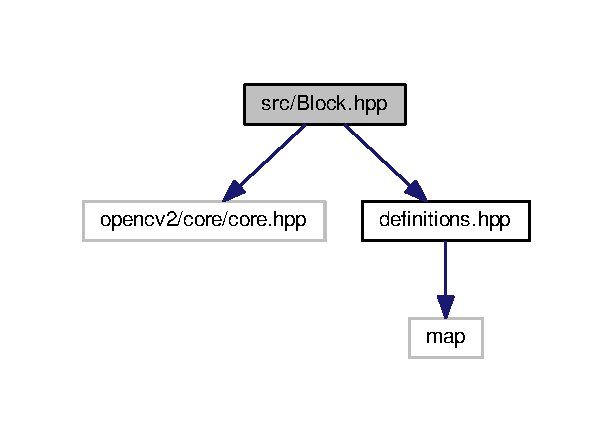
\includegraphics[width=294pt]{Block_8hpp__incl}
\end{center}
\end{figure}
This graph shows which files directly or indirectly include this file\+:
\nopagebreak
\begin{figure}[H]
\begin{center}
\leavevmode
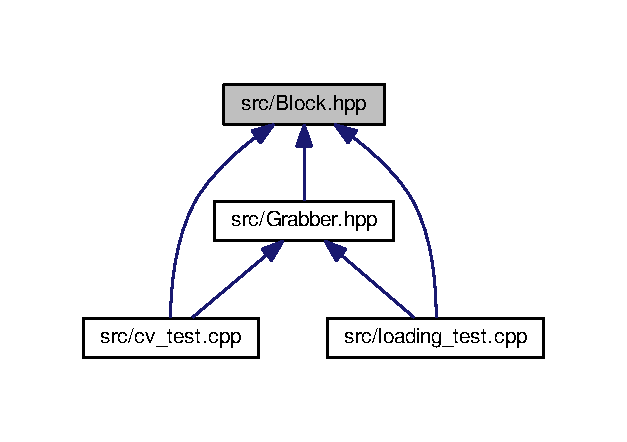
\includegraphics[width=301pt]{Block_8hpp__dep__incl}
\end{center}
\end{figure}
\subsection*{Classes}
\begin{DoxyCompactItemize}
\item 
class \hyperlink{classChipChipArray_1_1Block}{Chip\+Chip\+Array\+::\+Block}
\end{DoxyCompactItemize}
\subsection*{Namespaces}
\begin{DoxyCompactItemize}
\item 
 \hyperlink{namespaceChipChipArray}{Chip\+Chip\+Array}
\end{DoxyCompactItemize}


\subsection{Detailed Description}
Contains Block class. 

\begin{DoxyAuthor}{Author}
Samuel Andrew Wisner, \href{mailto:awisner94@gmail.com}{\tt awisner94@gmail.\+com} 
\end{DoxyAuthor}


Definition in file \hyperlink{Block_8hpp_source}{Block.\+hpp}.


\hypertarget{Block_8hpp_source}{\section{Block.\+hpp}
\label{Block_8hpp_source}\index{src/\+Block.\+hpp@{src/\+Block.\+hpp}}
}

\begin{DoxyCode}
00001 
00007 \textcolor{preprocessor}{#ifndef Block\_H}
00008 \textcolor{preprocessor}{#define Block\_H}
00009 
00010 \textcolor{preprocessor}{#include <opencv2/core/core.hpp>}
00011 
00012 \textcolor{preprocessor}{#include "\hyperlink{definitions_8hpp}{definitions.hpp}"}
00013 
00014 \textcolor{keyword}{namespace }\hyperlink{namespaceChipChipArray}{ChipChipArray} \{
\hypertarget{Block_8hpp_source_l00020}{}\hyperlink{classChipChipArray_1_1Block}{00020}     \textcolor{keyword}{class }\hyperlink{classChipChipArray_1_1Block}{Block} \{
00021         \textcolor{keyword}{public}:
\hypertarget{Block_8hpp_source_l00025}{}\hyperlink{classChipChipArray_1_1Block_ab5f9a9c1cc11e949685f8ad3d52599b2}{00025}             \hyperlink{definitions_8hpp_a1134b580f8da4de94ca6b1de4d37975e}{uint32} \hyperlink{classChipChipArray_1_1Block_ab5f9a9c1cc11e949685f8ad3d52599b2}{area};
00026 
\hypertarget{Block_8hpp_source_l00030}{}\hyperlink{classChipChipArray_1_1Block_a78304b597a8d8a74a4d9b4bb561a7224}{00030}             cv::Point \hyperlink{classChipChipArray_1_1Block_a78304b597a8d8a74a4d9b4bb561a7224}{bottomLeft};
00031 
\hypertarget{Block_8hpp_source_l00035}{}\hyperlink{classChipChipArray_1_1Block_a82f831883d31e6d74be45b8851eefe96}{00035}             cv::Point \hyperlink{classChipChipArray_1_1Block_a82f831883d31e6d74be45b8851eefe96}{bottomRight};
00036 
\hypertarget{Block_8hpp_source_l00041}{}\hyperlink{classChipChipArray_1_1Block_af3c4ecd0fd36763ac85c2dc0b57b8359}{00041}             \hyperlink{definitions_8hpp_a74df79fde3c518e55b29ce6360a9c76e}{sint16} \hyperlink{classChipChipArray_1_1Block_af3c4ecd0fd36763ac85c2dc0b57b8359}{dBottom};
00042 
\hypertarget{Block_8hpp_source_l00047}{}\hyperlink{classChipChipArray_1_1Block_aca89dc06d62feb9a6478a06976171b2b}{00047}             \hyperlink{definitions_8hpp_a74df79fde3c518e55b29ce6360a9c76e}{sint16} \hyperlink{classChipChipArray_1_1Block_aca89dc06d62feb9a6478a06976171b2b}{dLeft};
00048 
\hypertarget{Block_8hpp_source_l00053}{}\hyperlink{classChipChipArray_1_1Block_a6a4b0aa6aae7e41d836c8955e209c16e}{00053}             \hyperlink{definitions_8hpp_a74df79fde3c518e55b29ce6360a9c76e}{sint16} \hyperlink{classChipChipArray_1_1Block_a6a4b0aa6aae7e41d836c8955e209c16e}{dRight};
00054 
\hypertarget{Block_8hpp_source_l00059}{}\hyperlink{classChipChipArray_1_1Block_a4e792a05f677eafbeb9439a9e631c255}{00059}             \hyperlink{definitions_8hpp_a74df79fde3c518e55b29ce6360a9c76e}{sint16} \hyperlink{classChipChipArray_1_1Block_a4e792a05f677eafbeb9439a9e631c255}{dTop};
00060 
\hypertarget{Block_8hpp_source_l00067}{}\hyperlink{classChipChipArray_1_1Block_a5b6e72665d0de840a123717e24ca5cf9}{00067}             \hyperlink{definitions_8hpp_a74df79fde3c518e55b29ce6360a9c76e}{sint16} \hyperlink{classChipChipArray_1_1Block_a5b6e72665d0de840a123717e24ca5cf9}{dTopBottom};
00068 
\hypertarget{Block_8hpp_source_l00075}{}\hyperlink{classChipChipArray_1_1Block_a2d02c7b99ca656960fc9724587791999}{00075}             \hyperlink{definitions_8hpp_a74df79fde3c518e55b29ce6360a9c76e}{sint16} \hyperlink{classChipChipArray_1_1Block_a2d02c7b99ca656960fc9724587791999}{dRightLeft};
00076 
\hypertarget{Block_8hpp_source_l00082}{}\hyperlink{classChipChipArray_1_1Block_a42e2ca0775dc09b04049a2db1bc0bb4f}{00082}             \hyperlink{definitions_8hpp_a74df79fde3c518e55b29ce6360a9c76e}{sint16} \hyperlink{classChipChipArray_1_1Block_a42e2ca0775dc09b04049a2db1bc0bb4f}{offset};
00083 
\hypertarget{Block_8hpp_source_l00087}{}\hyperlink{classChipChipArray_1_1Block_aed94802c166c9b4553764eb637717a2a}{00087}             \hyperlink{definitions_8hpp_a05f6b0ae8f6a6e135b0e290c25fe0e4e}{uint16} \hyperlink{classChipChipArray_1_1Block_aed94802c166c9b4553764eb637717a2a}{height};
00088 
\hypertarget{Block_8hpp_source_l00092}{}\hyperlink{classChipChipArray_1_1Block_aeecc05025c6c8e23ff6ca09a6fbd4b4b}{00092}             cv::Point \hyperlink{classChipChipArray_1_1Block_aeecc05025c6c8e23ff6ca09a6fbd4b4b}{topLeft};
00093 
\hypertarget{Block_8hpp_source_l00097}{}\hyperlink{classChipChipArray_1_1Block_aaa4ff82846e95a628800ebdfd3ceefb5}{00097}             cv::Point \hyperlink{classChipChipArray_1_1Block_aaa4ff82846e95a628800ebdfd3ceefb5}{topRight};
00098 
\hypertarget{Block_8hpp_source_l00102}{}\hyperlink{classChipChipArray_1_1Block_ac3f815e8aa9060c4ad20d4e1b2649e35}{00102}             \hyperlink{definitions_8hpp_a05f6b0ae8f6a6e135b0e290c25fe0e4e}{uint16} \hyperlink{classChipChipArray_1_1Block_ac3f815e8aa9060c4ad20d4e1b2649e35}{width};
00103 
\hypertarget{Block_8hpp_source_l00107}{}\hyperlink{classChipChipArray_1_1Block_a262210a9a04028f3f2670c9ae38ef3d7}{00107}             \hyperlink{definitions_8hpp_abc05a0f46084a3477cf5d5c939ff1436}{Color} \hyperlink{classChipChipArray_1_1Block_a262210a9a04028f3f2670c9ae38ef3d7}{color};
00108 
\hypertarget{Block_8hpp_source_l00112}{}\hyperlink{classChipChipArray_1_1Block_aebd356d7fcfe7ff11db8195e6d7f8e42}{00112}             \hyperlink{definitions_8hpp_a9809446fd16a744b6df9808293f14153}{Size} \hyperlink{classChipChipArray_1_1Block_aebd356d7fcfe7ff11db8195e6d7f8e42}{size};
00113 
00119             \hyperlink{classChipChipArray_1_1Block_a7eb2456e5c95c8a91844c9522eed0578}{Block}(cv::Rect rect, \hyperlink{definitions_8hpp_abc05a0f46084a3477cf5d5c939ff1436}{Color} color);
00120 
00121         \textcolor{keyword}{private}:
00125             \textcolor{keyword}{static} \textcolor{keyword}{const} \hyperlink{definitions_8hpp_a05f6b0ae8f6a6e135b0e290c25fe0e4e}{uint16} IMG\_HEIGHT = 1280;
00126 
00130             \textcolor{keyword}{static} \textcolor{keyword}{const} \hyperlink{definitions_8hpp_a05f6b0ae8f6a6e135b0e290c25fe0e4e}{uint16} IMG\_WIDTH = 720;
00131 
00136             \textcolor{keyword}{static} \textcolor{keyword}{const} \hyperlink{definitions_8hpp_a1134b580f8da4de94ca6b1de4d37975e}{uint32} MIN\_WHOLE\_BLOCK\_SIZE = 50000;
00137     \};
00138 
\hypertarget{Block_8hpp_source_l00139}{}\hyperlink{classChipChipArray_1_1Block_a7eb2456e5c95c8a91844c9522eed0578}{00139}     \hyperlink{classChipChipArray_1_1Block_a7eb2456e5c95c8a91844c9522eed0578}{Block::Block}(cv::Rect rect, \hyperlink{definitions_8hpp_abc05a0f46084a3477cf5d5c939ff1436}{Color} color) \{
00140         \textcolor{comment}{// basic geometric properties}
00141         \hyperlink{classChipChipArray_1_1Block_ab5f9a9c1cc11e949685f8ad3d52599b2}{area} = rect.area();
00142         \hyperlink{classChipChipArray_1_1Block_aed94802c166c9b4553764eb637717a2a}{height} = rect.height;
00143         \hyperlink{classChipChipArray_1_1Block_ac3f815e8aa9060c4ad20d4e1b2649e35}{width} = rect.width;
00144 
00145         \textcolor{comment}{// assigning corners}
00146         \hyperlink{classChipChipArray_1_1Block_aeecc05025c6c8e23ff6ca09a6fbd4b4b}{topLeft} = rect.tl();
00147         \hyperlink{classChipChipArray_1_1Block_a82f831883d31e6d74be45b8851eefe96}{bottomRight} = rect.br();
00148         \hyperlink{classChipChipArray_1_1Block_aaa4ff82846e95a628800ebdfd3ceefb5}{topRight} = cv::Point(\hyperlink{classChipChipArray_1_1Block_aeecc05025c6c8e23ff6ca09a6fbd4b4b}{topLeft}.x + \hyperlink{classChipChipArray_1_1Block_ac3f815e8aa9060c4ad20d4e1b2649e35}{width}, \hyperlink{classChipChipArray_1_1Block_aeecc05025c6c8e23ff6ca09a6fbd4b4b}{topLeft}.y);
00149         \hyperlink{classChipChipArray_1_1Block_a78304b597a8d8a74a4d9b4bb561a7224}{bottomLeft} = cv::Point(\hyperlink{classChipChipArray_1_1Block_aeecc05025c6c8e23ff6ca09a6fbd4b4b}{topLeft}.x, \hyperlink{classChipChipArray_1_1Block_aeecc05025c6c8e23ff6ca09a6fbd4b4b}{topLeft}.y + 
      \hyperlink{classChipChipArray_1_1Block_aed94802c166c9b4553764eb637717a2a}{height});
00150         \hyperlink{classChipChipArray_1_1Block_a42e2ca0775dc09b04049a2db1bc0bb4f}{offset} = (\hyperlink{definitions_8hpp_a74df79fde3c518e55b29ce6360a9c76e}{sint16})(\hyperlink{classChipChipArray_1_1Block_aeecc05025c6c8e23ff6ca09a6fbd4b4b}{topLeft}.x + \hyperlink{classChipChipArray_1_1Block_ac3f815e8aa9060c4ad20d4e1b2649e35}{width} / 2) - IMG\_WIDTH / 2;
00151 
00152         \textcolor{comment}{// calculating offsets (opencv low coordinates start top left)}
00153         \hyperlink{classChipChipArray_1_1Block_aca89dc06d62feb9a6478a06976171b2b}{dLeft} = \hyperlink{classChipChipArray_1_1Block_aeecc05025c6c8e23ff6ca09a6fbd4b4b}{topLeft}.x;
00154         \hyperlink{classChipChipArray_1_1Block_a6a4b0aa6aae7e41d836c8955e209c16e}{dRight} = IMG\_WIDTH - \hyperlink{classChipChipArray_1_1Block_aaa4ff82846e95a628800ebdfd3ceefb5}{topRight}.x;
00155         \hyperlink{classChipChipArray_1_1Block_a4e792a05f677eafbeb9439a9e631c255}{dTop} = \hyperlink{classChipChipArray_1_1Block_aeecc05025c6c8e23ff6ca09a6fbd4b4b}{topLeft}.y;
00156         \hyperlink{classChipChipArray_1_1Block_af3c4ecd0fd36763ac85c2dc0b57b8359}{dBottom} = IMG\_HEIGHT - \hyperlink{classChipChipArray_1_1Block_a82f831883d31e6d74be45b8851eefe96}{bottomRight}.y;
00157         \hyperlink{classChipChipArray_1_1Block_a5b6e72665d0de840a123717e24ca5cf9}{dTopBottom} = \hyperlink{classChipChipArray_1_1Block_a4e792a05f677eafbeb9439a9e631c255}{dTop} - \hyperlink{classChipChipArray_1_1Block_af3c4ecd0fd36763ac85c2dc0b57b8359}{dBottom};
00158         \hyperlink{classChipChipArray_1_1Block_a2d02c7b99ca656960fc9724587791999}{dRightLeft} = \hyperlink{classChipChipArray_1_1Block_a6a4b0aa6aae7e41d836c8955e209c16e}{dRight} - \hyperlink{classChipChipArray_1_1Block_aca89dc06d62feb9a6478a06976171b2b}{dLeft};
00159 
00160         \textcolor{comment}{// set color and size}
00161         this->color = \hyperlink{classChipChipArray_1_1Block_a262210a9a04028f3f2670c9ae38ef3d7}{color};
00162         \hyperlink{classChipChipArray_1_1Block_aebd356d7fcfe7ff11db8195e6d7f8e42}{size} = \hyperlink{classChipChipArray_1_1Block_ab5f9a9c1cc11e949685f8ad3d52599b2}{area} > MIN\_WHOLE\_BLOCK\_SIZE ? \hyperlink{definitions_8hpp_a9809446fd16a744b6df9808293f14153a8394f0347c184cf156ac5924dccb773b}{Size::Long} : 
      \hyperlink{definitions_8hpp_a9809446fd16a744b6df9808293f14153a30bb747c98bccdd11b3f89e644c4d0ad}{Size::Short};
00163     \}
00164 \}
00165 \textcolor{preprocessor}{#endif}
\end{DoxyCode}

\hypertarget{cv__hue_8cpp}{\section{src/cv\+\_\+hue.cpp File Reference}
\label{cv__hue_8cpp}\index{src/cv\+\_\+hue.\+cpp@{src/cv\+\_\+hue.\+cpp}}
}
{\ttfamily \#include $<$iostream$>$}\\*
{\ttfamily \#include \char`\"{}opencv2/highgui/highgui.\+hpp\char`\"{}}\\*
{\ttfamily \#include \char`\"{}opencv2/imgproc/imgproc.\+hpp\char`\"{}}\\*
{\ttfamily \#include \char`\"{}Pi\+Camera.\+hpp\char`\"{}}\\*
Include dependency graph for cv\+\_\+hue.\+cpp\+:
\nopagebreak
\begin{figure}[H]
\begin{center}
\leavevmode
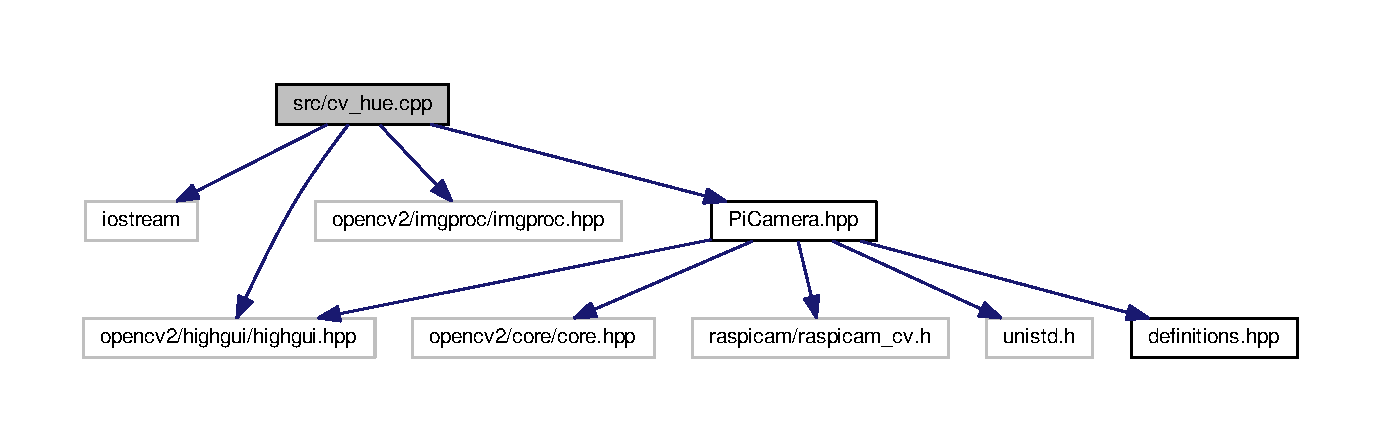
\includegraphics[width=350pt]{cv__hue_8cpp__incl}
\end{center}
\end{figure}
\subsection*{Namespaces}
\begin{DoxyCompactItemize}
\item 
 \hyperlink{namespaceChipChipArray}{Chip\+Chip\+Array}
\begin{DoxyCompactList}\small\item\em contains \hyperlink{classChipChipArray_1_1Block}{Block} class \end{DoxyCompactList}\end{DoxyCompactItemize}
\subsection*{Functions}
\begin{DoxyCompactItemize}
\item 
int \hyperlink{namespaceChipChipArray_a7fc3d1edffca11531cd09fdab7c8b88d}{Chip\+Chip\+Array\+::main} (int argc, char $\ast$$\ast$argv)
\end{DoxyCompactItemize}

\hypertarget{cv__hue_8cpp_source}{\section{cv\+\_\+hue.\+cpp}
\label{cv__hue_8cpp_source}\index{src/cv\+\_\+hue.\+cpp@{src/cv\+\_\+hue.\+cpp}}
}

\begin{DoxyCode}
00001 
00008 \textcolor{preprocessor}{#include <iostream>}
00009 \textcolor{preprocessor}{#include "opencv2/highgui/highgui.hpp"}
00010 \textcolor{preprocessor}{#include "opencv2/imgproc/imgproc.hpp"}
00011 
00012 \textcolor{preprocessor}{#include "\hyperlink{PiCamera_8hpp}{PiCamera.hpp}"}
00013 
00014 \textcolor{keyword}{using namespace }\hyperlink{namespacecv}{cv};
00015 \textcolor{keyword}{using namespace }\hyperlink{namespacestd}{std};
00016 \textcolor{keyword}{using namespace }\hyperlink{namespaceChipChipArray}{ChipChipArray};
00017 
00018 \textcolor{keyword}{namespace }\hyperlink{namespaceChipChipArray}{ChipChipArray} \{
00019     
\hypertarget{cv__hue_8cpp_source_l00027}{}\hyperlink{namespaceChipChipArray_a7fc3d1edffca11531cd09fdab7c8b88d}{00027}     \textcolor{keywordtype}{int} \hyperlink{namespaceChipChipArray_a7fc3d1edffca11531cd09fdab7c8b88d}{main}( \textcolor{keywordtype}{int} argc, \textcolor{keywordtype}{char}** argv ) \{
00028         \hyperlink{classChipChipArray_1_1PiCamera}{PiCamera} cam;
00029         namedWindow(\textcolor{stringliteral}{"Control"}, CV\_WINDOW\_AUTOSIZE); \textcolor{comment}{//create a window called "Control"}
00030 
00031         \textcolor{keywordtype}{int} iLowH = 170;
00032         \textcolor{keywordtype}{int} iHighH = 179;
00033 
00034         \textcolor{keywordtype}{int} iLowS = 150; 
00035         \textcolor{keywordtype}{int} iHighS = 255;
00036 
00037         \textcolor{keywordtype}{int} iLowV = 60;
00038         \textcolor{keywordtype}{int} iHighV = 255;
00039 
00040         \textcolor{comment}{//Create trackbars in "Control" window}
00041         createTrackbar(\textcolor{stringliteral}{"LowH"}, \textcolor{stringliteral}{"Control"}, &iLowH, 179); \textcolor{comment}{//Hue (0 - 179)}
00042         createTrackbar(\textcolor{stringliteral}{"HighH"}, \textcolor{stringliteral}{"Control"}, &iHighH, 179);
00043 
00044         createTrackbar(\textcolor{stringliteral}{"LowS"}, \textcolor{stringliteral}{"Control"}, &iLowS, 255); \textcolor{comment}{//Saturation (0 - 255)}
00045         createTrackbar(\textcolor{stringliteral}{"HighS"}, \textcolor{stringliteral}{"Control"}, &iHighS, 255);
00046 
00047         createTrackbar(\textcolor{stringliteral}{"LowV"}, \textcolor{stringliteral}{"Control"}, &iLowV, 255);\textcolor{comment}{//Value (0 - 255)}
00048         createTrackbar(\textcolor{stringliteral}{"HighV"}, \textcolor{stringliteral}{"Control"}, &iHighV, 255);
00049 
00050         \textcolor{keywordtype}{int} iLastX = -1; 
00051         \textcolor{keywordtype}{int} iLastY = -1;
00052 
00053         \textcolor{comment}{//Capture a temporary image from the camera}
00054         Mat imgTmp = cam.\hyperlink{classChipChipArray_1_1PiCamera_a58fb0de02570dce9a9cb60a1a04fb84f}{Snap}();
00055 
00056         \textcolor{comment}{//Create a black image with the size as the camera output}
00057         Mat imgLines = Mat::zeros( imgTmp.size(), CV\_8UC3 );;
00058 
00059 
00060         \textcolor{keywordflow}{while} (\textcolor{keyword}{true})
00061         \{
00062             Mat imgOriginal = cam.\hyperlink{classChipChipArray_1_1PiCamera_a58fb0de02570dce9a9cb60a1a04fb84f}{Snap}(); \textcolor{comment}{// read a new frame from video}
00063             Mat imgHSV;
00064 
00065             cvtColor(imgOriginal, imgHSV, COLOR\_BGR2HSV); \textcolor{comment}{//Convert the captured frame from BGR to HSV}
00066 
00067             Mat imgThresholded;
00068 
00069             inRange(imgHSV, Scalar(iLowH, iLowS, iLowV), Scalar(iHighH, iHighS, iHighV), imgThresholded); \textcolor{comment}{
      //Threshold the image}
00070 
00071             \textcolor{comment}{//morphological opening (removes small objects from the foreground)}
00072             erode(imgThresholded, imgThresholded, getStructuringElement(MORPH\_ELLIPSE, 
      \hyperlink{definitions_8hpp_a9809446fd16a744b6df9808293f14153}{Size}(5, 5)) );
00073             dilate( imgThresholded, imgThresholded, getStructuringElement(MORPH\_ELLIPSE, 
      \hyperlink{definitions_8hpp_a9809446fd16a744b6df9808293f14153}{Size}(5, 5)) ); 
00074 
00075             \textcolor{comment}{//morphological closing (removes small holes from the foreground)}
00076             dilate( imgThresholded, imgThresholded, getStructuringElement(MORPH\_ELLIPSE, 
      \hyperlink{definitions_8hpp_a9809446fd16a744b6df9808293f14153}{Size}(5, 5)) ); 
00077             erode(imgThresholded, imgThresholded, getStructuringElement(MORPH\_ELLIPSE, 
      \hyperlink{definitions_8hpp_a9809446fd16a744b6df9808293f14153}{Size}(5, 5)) );
00078 
00079             \textcolor{comment}{//Calculate the moments of the thresholded image}
00080             Moments oMoments = moments(imgThresholded);
00081 
00082             \textcolor{comment}{/*double dM01 = oMoments.m01;}
00083 \textcolor{comment}{              double dM10 = oMoments.m10;}
00084 \textcolor{comment}{              double dArea = oMoments.m00;}
00085 \textcolor{comment}{}
00086 \textcolor{comment}{            // if the area <= 10000, I consider that the there are no object in the image and it's because
       of the noise, the area is not zero }
00087 \textcolor{comment}{            if (dArea > 50000)}
00088 \textcolor{comment}{            \{}
00089 \textcolor{comment}{            //calculate the position of the ball}
00090 \textcolor{comment}{            int posX = dM10 / dArea;}
00091 \textcolor{comment}{            int posY = dM01 / dArea;        }
00092 \textcolor{comment}{}
00093 \textcolor{comment}{            if (iLastX >= 0 && iLastY >= 0 && posX >= 0 && posY >= 0)}
00094 \textcolor{comment}{            \{}
00095 \textcolor{comment}{            //Draw a red line from the previous point to the current point}
00096 \textcolor{comment}{            line(imgLines, Point(posX, posY), Point(iLastX, iLastY), Scalar(0,0,255), 2);}
00097 \textcolor{comment}{            \}}
00098 \textcolor{comment}{}
00099 \textcolor{comment}{            iLastX = posX;}
00100 \textcolor{comment}{            iLastY = posY;}
00101 \textcolor{comment}{            \}}
00102 \textcolor{comment}{            */}
00103             imshow(\textcolor{stringliteral}{"Thresholded Image"}, imgThresholded); \textcolor{comment}{//show the thresholded image}
00104 
00105             \textcolor{comment}{//      imgOriginal = imgOriginal + imgLines;}
00106             imshow(\textcolor{stringliteral}{"Original"}, imgOriginal); \textcolor{comment}{//show the original image}
00107 
00108             \textcolor{keywordflow}{if} (waitKey(30) == 27) \textcolor{comment}{//wait for 'esc' key press for 30ms. If 'esc' key is pressed, break loop}
00109             \{
00110                 cout << \textcolor{stringliteral}{"esc key is pressed by user"} << endl;
00111                 \textcolor{keywordflow}{break}; 
00112             \}
00113         \}
00114 
00115         \textcolor{keywordflow}{return} 0;
00116     \}
00117 \}
\end{DoxyCode}

\hypertarget{cv__shape_8cpp}{\section{src/cv\+\_\+shape.cpp File Reference}
\label{cv__shape_8cpp}\index{src/cv\+\_\+shape.\+cpp@{src/cv\+\_\+shape.\+cpp}}
}
{\ttfamily \#include $<$iostream$>$}\\*
{\ttfamily \#include $<$opencv2/highgui/highgui.\+hpp$>$}\\*
{\ttfamily \#include $<$opencv2/imgproc/imgproc.\+hpp$>$}\\*
{\ttfamily \#include $<$string$>$}\\*
{\ttfamily \#include \char`\"{}definitions.\+hpp\char`\"{}}\\*
{\ttfamily \#include \char`\"{}Pi\+Camera.\+hpp\char`\"{}}\\*
Include dependency graph for cv\+\_\+shape.\+cpp\+:
\nopagebreak
\begin{figure}[H]
\begin{center}
\leavevmode
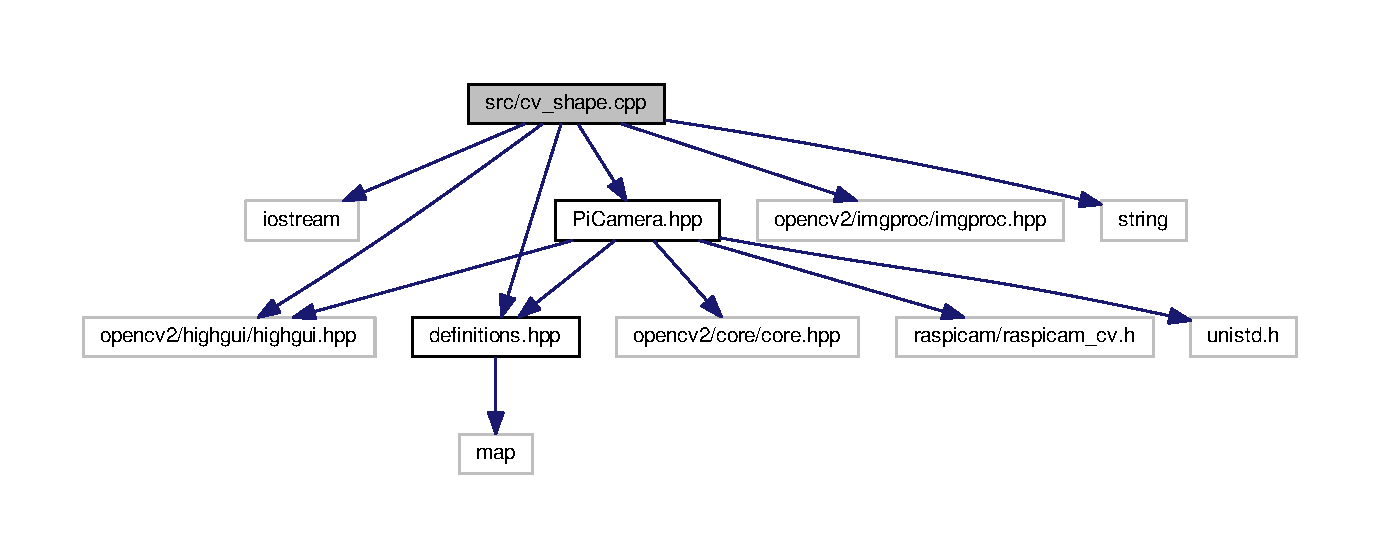
\includegraphics[width=350pt]{cv__shape_8cpp__incl}
\end{center}
\end{figure}
\subsection*{Functions}
\begin{DoxyCompactItemize}
\item 
int \hyperlink{cv__shape_8cpp_ae66f6b31b5ad750f1fe042a706a4e3d4}{main} ()
\end{DoxyCompactItemize}


\subsection{Function Documentation}
\hypertarget{cv__shape_8cpp_ae66f6b31b5ad750f1fe042a706a4e3d4}{\index{cv\+\_\+shape.\+cpp@{cv\+\_\+shape.\+cpp}!main@{main}}
\index{main@{main}!cv\+\_\+shape.\+cpp@{cv\+\_\+shape.\+cpp}}
\subsubsection[{main}]{\setlength{\rightskip}{0pt plus 5cm}int main (
\begin{DoxyParamCaption}
{}
\end{DoxyParamCaption}
)}}\label{cv__shape_8cpp_ae66f6b31b5ad750f1fe042a706a4e3d4}
This program (a single function) is a test of the computer vision algorithms for loading the blocks. It will likely be in development for some time to come. The plan currently is to develop and test all C\+V algorithms for block loading here before moving it all into class functions and testing again.

This code is based on several online articles\+:
\begin{DoxyItemize}
\item \char`\"{}\+Color Detectionn \& Object Tracking\char`\"{} by Shermal Fernando (\href{http://opencv-srf.blogspot.com/2010/09/object-detection-using-color-seperation.html}{\tt http\+://opencv-\/srf.\+blogspot.\+com/2010/09/object-\/detection-\/using-\/color-\/seperation.\+html})
\item \char`\"{}\+Shape Detection \& Tracking using Contours\char`\"{} by Shermal Fernando (\href{http://opencv-srf.blogspot.com/2011/09/object-detection-tracking-using-contours.html}{\tt http\+://opencv-\/srf.\+blogspot.\+com/2011/09/object-\/detection-\/tracking-\/using-\/contours.\+html})
\item \char`\"{}\+Creating Bounding boxes and circles for contours\char`\"{} in the Open\+C\+V 2.\+4 Tutorials (\href{http://opencv-srf.blogspot.com/2011/09/object-detection-tracking-using-contours.html}{\tt http\+://opencv-\/srf.\+blogspot.\+com/2011/09/object-\/detection-\/tracking-\/using-\/contours.\+html}) 
\end{DoxyItemize}

Definition at line 36 of file cv\+\_\+shape.\+cpp.



Here is the call graph for this function\+:
\nopagebreak
\begin{figure}[H]
\begin{center}
\leavevmode
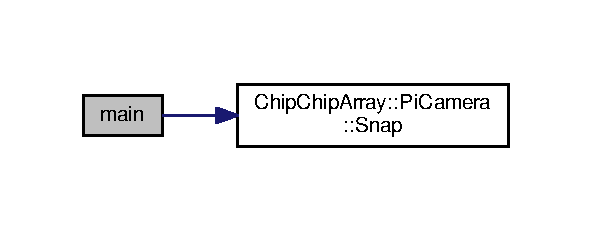
\includegraphics[width=284pt]{cv__shape_8cpp_ae66f6b31b5ad750f1fe042a706a4e3d4_cgraph}
\end{center}
\end{figure}



\hypertarget{cv__shape_8cpp_source}{\section{cv\+\_\+shape.\+cpp}
\label{cv__shape_8cpp_source}\index{src/cv\+\_\+shape.\+cpp@{src/cv\+\_\+shape.\+cpp}}
}

\begin{DoxyCode}
00001 
00008 \textcolor{preprocessor}{#include <iostream>}
00009 \textcolor{preprocessor}{#include <opencv2/highgui/highgui.hpp>}
00010 \textcolor{preprocessor}{#include <opencv2/imgproc/imgproc.hpp>}
00011 \textcolor{preprocessor}{#include <string>}
00012 
00013 \textcolor{preprocessor}{#include "\hyperlink{definitions_8hpp}{definitions.hpp}"}
00014 \textcolor{preprocessor}{#include "\hyperlink{PiCamera_8hpp}{PiCamera.hpp}"}
00015 
00016 \textcolor{keyword}{using namespace }\hyperlink{namespaceChipChipArray}{ChipChipArray};
00017 \textcolor{keyword}{using namespace }\hyperlink{namespacecv}{cv};
00018 \textcolor{keyword}{using namespace }\hyperlink{namespacestd}{std};
00019 
\hypertarget{cv__shape_8cpp_source_l00037}{}\hyperlink{cv__shape_8cpp_ae66f6b31b5ad750f1fe042a706a4e3d4}{00037} \textcolor{keywordtype}{int} \hyperlink{namespaceChipChipArray_a7fc3d1edffca11531cd09fdab7c8b88d}{main}() \{
00038     \hyperlink{classChipChipArray_1_1PiCamera}{PiCamera} cam;
00039 
00040     \textcolor{comment}{// window names}
00041     \textcolor{keywordtype}{string} control = \textcolor{stringliteral}{"Settings"};
00042     \textcolor{keywordtype}{string} winThresh = \textcolor{stringliteral}{"Image Threshold"};
00043     \textcolor{keywordtype}{string} winContours = \textcolor{stringliteral}{"Contours Detected"};
00044 
00045     \textcolor{comment}{// control (trackbar) variables}
00046     \textcolor{keywordtype}{int} lowH = 0;  \textcolor{comment}{// hue}
00047     \textcolor{keywordtype}{int} highH = 255;
00048     \textcolor{keywordtype}{int} lowS = 0;  \textcolor{comment}{// saturation}
00049     \textcolor{keywordtype}{int} highS = 255;
00050     \textcolor{keywordtype}{int} lowV = 0;  \textcolor{comment}{// value}
00051     \textcolor{keywordtype}{int} highV = 255;
00052     \textcolor{keywordtype}{int} polyEps = 3;  \textcolor{comment}{// max dif b/t bin shape edge & est poly edge}
00053 
00054     \textcolor{comment}{// opening windows}
00055     namedWindow(control, CV\_WINDOW\_AUTOSIZE);
00056     namedWindow(winThresh, CV\_WINDOW\_AUTOSIZE);
00057     namedWindow(winContours, CV\_WINDOW\_AUTOSIZE);
00058 
00059     \textcolor{comment}{// creating control trackbars}
00060     createTrackbar(\textcolor{stringliteral}{"Hue Min"}, control, &lowH, highH);
00061     createTrackbar(\textcolor{stringliteral}{"Hue Max"}, control, &highH, highH);
00062     createTrackbar(\textcolor{stringliteral}{"Sat Min"}, control, &lowS, highS);
00063     createTrackbar(\textcolor{stringliteral}{"Sat Max"}, control, &highS, highS);
00064     createTrackbar(\textcolor{stringliteral}{"Val Min"}, control, &lowV, highV);
00065     createTrackbar(\textcolor{stringliteral}{"Val Max"}, control, &highV, highV);
00066     createTrackbar(\textcolor{stringliteral}{"Polygon Epsilon"}, control, &polyEps, 20);
00067 
00068     \textcolor{keywordflow}{while}(\textcolor{keyword}{true}) \{
00069         Mat imgOrig = cam.\hyperlink{classChipChipArray_1_1PiCamera_a58fb0de02570dce9a9cb60a1a04fb84f}{Snap}();  \textcolor{comment}{// real iage}
00070         Mat imgHSV;  \textcolor{comment}{// RGB image converted to HSV space}
00071         Mat imgThresh;  \textcolor{comment}{// binary threshold image}
00072         \textcolor{comment}{//cvtColor(imgOrig, imgHSV, CV\_BGR2YUV);}
00073         \textcolor{comment}{//cvtColor(imgHSV, imgOrig, CV\_HSV2BGR);}
00074         cvtColor(imgOrig, imgHSV, COLOR\_BGR2HSV);
00075 
00076         \textcolor{comment}{// create binary image}
00077         inRange(imgHSV, Scalar(lowH, lowS, lowV), Scalar(highH, highS,
00078                     highV), imgThresh);
00079 
00080         \textcolor{comment}{/* }
00081 \textcolor{comment}{         * Not quite sure what all this does, but it seems to}
00082 \textcolor{comment}{         * relate to smoothing the image}
00083 \textcolor{comment}{         */}
00084         erode(imgThresh, imgThresh, getStructuringElement(
00085                     MORPH\_ELLIPSE, \hyperlink{definitions_8hpp_a9809446fd16a744b6df9808293f14153}{cv::Size}(5, 5)));
00086         dilate(imgThresh, imgThresh, getStructuringElement(
00087                     MORPH\_ELLIPSE, \hyperlink{definitions_8hpp_a9809446fd16a744b6df9808293f14153}{cv::Size}(5, 5)));
00088         dilate(imgThresh, imgThresh, getStructuringElement(
00089                     MORPH\_ELLIPSE, \hyperlink{definitions_8hpp_a9809446fd16a744b6df9808293f14153}{cv::Size}(5, 5)));
00090         erode(imgThresh, imgThresh, getStructuringElement(
00091                     MORPH\_ELLIPSE, \hyperlink{definitions_8hpp_a9809446fd16a744b6df9808293f14153}{cv::Size}(5, 5)));
00092 
00093         \textcolor{comment}{// show binary image in threshold window}
00094         imshow(winThresh, imgThresh);
00095 
00096         \textcolor{comment}{// calculate contours}
00097         vector<vector<Point>> contours;
00098         findContours(imgThresh, contours, CV\_RETR\_TREE,
00099                 CV\_CHAIN\_APPROX\_SIMPLE, Point(0, 0));
00100         vector<vector<Point>> contours\_poly(contours.size());
00101         vector<Rect> bounds(contours.size());
00102         \textcolor{keywordtype}{int} maxArea = 0;
00103         \textcolor{keywordtype}{int} offset;
00104 
00105         \textcolor{comment}{// find rectangle around polygon-ish shapes}
00106         \textcolor{keywordflow}{for}(\textcolor{keywordtype}{int} i = 0; i < contours.size(); i++) \{
00107             approxPolyDP(Mat(contours[i]), contours\_poly[i],
00108                     polyEps, \textcolor{keyword}{false});
00109             bounds[i] = boundingRect(Mat(contours\_poly[i]));
00110         \}
00111 
00112         \textcolor{comment}{/* }
00113 \textcolor{comment}{         * Draw surrounding rectangles from above on original}
00114 \textcolor{comment}{         * image.}
00115 \textcolor{comment}{         */}
00116         \textcolor{keywordflow}{for}(\textcolor{keywordtype}{int} i = 0; i < contours.size(); i++) \{
00117             rectangle(imgOrig, bounds[i].tl(), bounds[i].br(),
00118                     Scalar(255, 0, 0), 2, 8, 0);
00119             \textcolor{comment}{//drawContours(imgOrig, contours\_poly, i,}
00120             \textcolor{comment}{//      Scalar(255, 0, 0), 4, 8);}
00121             \textcolor{keywordtype}{int} area = bounds[i].width * bounds[i].height;
00122 
00123             \textcolor{keywordflow}{if}(area > maxArea) \{
00124                 offset = abs(640 - (bounds[i].tl().x + bounds[i].width / 2));
00125                 maxArea = area;
00126             \}
00127         \}
00128 
00129         cout << \textcolor{stringliteral}{"Block area: "} << maxArea << \textcolor{stringliteral}{" pixels\(\backslash\)t\(\backslash\)t"} 
00130             << \textcolor{stringliteral}{"Center offset: "} << offset << endl;
00131         imshow(winContours, imgOrig);  \textcolor{comment}{// show original image with rectangles}
00132         waitKey(50);  \textcolor{comment}{// has to be here :(}
00133     \}
00134 \}
\end{DoxyCode}

\hypertarget{cv__test_8cpp}{\section{src/cv\+\_\+test.cpp File Reference}
\label{cv__test_8cpp}\index{src/cv\+\_\+test.\+cpp@{src/cv\+\_\+test.\+cpp}}
}
{\ttfamily \#include $<$iostream$>$}\\*
{\ttfamily \#include \char`\"{}definitions.\+hpp\char`\"{}}\\*
{\ttfamily \#include \char`\"{}Block.\+hpp\char`\"{}}\\*
{\ttfamily \#include \char`\"{}Grabber.\+hpp\char`\"{}}\\*
Include dependency graph for cv\+\_\+test.\+cpp\+:
\nopagebreak
\begin{figure}[H]
\begin{center}
\leavevmode
\includegraphics[width=350pt]{cv__test_8cpp__incl}
\end{center}
\end{figure}
\subsection*{Functions}
\begin{DoxyCompactItemize}
\item 
int \hyperlink{cv__test_8cpp_ae66f6b31b5ad750f1fe042a706a4e3d4}{main} ()
\end{DoxyCompactItemize}


\subsection{Function Documentation}
\hypertarget{cv__test_8cpp_ae66f6b31b5ad750f1fe042a706a4e3d4}{\index{cv\+\_\+test.\+cpp@{cv\+\_\+test.\+cpp}!main@{main}}
\index{main@{main}!cv\+\_\+test.\+cpp@{cv\+\_\+test.\+cpp}}
\subsubsection[{main}]{\setlength{\rightskip}{0pt plus 5cm}int main (
\begin{DoxyParamCaption}
{}
\end{DoxyParamCaption}
)}}\label{cv__test_8cpp_ae66f6b31b5ad750f1fe042a706a4e3d4}
This program was used solely to test the Pi\+Camera wrapper class and its compatibility with the raspicam wrapper and ultimately Open\+C\+V. 

Definition at line 18 of file cv\+\_\+test.\+cpp.



Here is the call graph for this function\+:
\nopagebreak
\begin{figure}[H]
\begin{center}
\leavevmode
\includegraphics[width=350pt]{cv__test_8cpp_ae66f6b31b5ad750f1fe042a706a4e3d4_cgraph}
\end{center}
\end{figure}



\hypertarget{cv__test_8cpp_source}{\section{cv\+\_\+test.\+cpp}
\label{cv__test_8cpp_source}\index{src/cv\+\_\+test.\+cpp@{src/cv\+\_\+test.\+cpp}}
}

\begin{DoxyCode}
00001 
00007 \textcolor{preprocessor}{#include <iostream>}
00008 
00009 \textcolor{preprocessor}{#include "\hyperlink{definitions_8hpp}{definitions.hpp}"}
00010 \textcolor{preprocessor}{#include "\hyperlink{Block_8hpp}{Block.hpp}"}
00011 \textcolor{preprocessor}{#include "\hyperlink{Grabber_8hpp}{Grabber.hpp}"}
00012 
00013 \textcolor{keyword}{using namespace }\hyperlink{namespaceChipChipArray}{ChipChipArray};
00014 
\hypertarget{cv__test_8cpp_source_l00019}{}\hyperlink{cv__test_8cpp_ae66f6b31b5ad750f1fe042a706a4e3d4}{00019} \textcolor{keywordtype}{int} \hyperlink{namespaceChipChipArray_a7fc3d1edffca11531cd09fdab7c8b88d}{main}() \{
00020     \hyperlink{classChipChipArray_1_1Grabber}{Grabber} g(\hyperlink{definitions_8hpp_adbd1e7a33d3e1751c7b2aa2562d0ecb9a0d61f8370cad1d412f80b84d143e1257}{Zone::C}, \hyperlink{definitions_8hpp_a03325a8a9d4f105db5e37dd587128142a945d5e233cf7d6240f6b783b36a374ff}{Side::Left});
00021     \hyperlink{classChipChipArray_1_1Block}{Block} block = g.LocateBlock();
00022     g.\hyperlink{classChipChipArray_1_1Grabber_aacf089ceb4aa5b263c2cc702fb3daf74}{Close}();
00023     std::cout << \hyperlink{namespacestd_aa5ddf582a1c96ffe258c997be9a294a3}{std::to\_string}(block.\hyperlink{classChipChipArray_1_1Block_a262210a9a04028f3f2670c9ae38ef3d7}{color}) << std::endl;
00024     std::cout << \textcolor{stringliteral}{"Offset: "} << block.\hyperlink{classChipChipArray_1_1Block_a42e2ca0775dc09b04049a2db1bc0bb4f}{offset} << std::endl;
00025 
00026     \hyperlink{classChipChipArray_1_1Grabber}{Grabber} g2(\hyperlink{definitions_8hpp_adbd1e7a33d3e1751c7b2aa2562d0ecb9a9d5ed678fe57bcca610140957afab571}{Zone::B}, \hyperlink{definitions_8hpp_a03325a8a9d4f105db5e37dd587128142a92b09c7c48c520c3c55e497875da437c}{Side::Right});
00027     \hyperlink{classChipChipArray_1_1Block}{Block} block2 = g2.LocateBlock();
00028     g2.\hyperlink{classChipChipArray_1_1Grabber_aacf089ceb4aa5b263c2cc702fb3daf74}{Close}();
00029     std::cout << \hyperlink{namespacestd_aa5ddf582a1c96ffe258c997be9a294a3}{std::to\_string}(block2.\hyperlink{classChipChipArray_1_1Block_a262210a9a04028f3f2670c9ae38ef3d7}{color}) << std::endl;
00030     std::cout << \textcolor{stringliteral}{"Offset: "} << block2.\hyperlink{classChipChipArray_1_1Block_a42e2ca0775dc09b04049a2db1bc0bb4f}{offset} << std::endl;
00031 
00032 \}
\end{DoxyCode}

\hypertarget{dark__magic_8cpp}{\section{src/dark\+\_\+magic.cpp File Reference}
\label{dark__magic_8cpp}\index{src/dark\+\_\+magic.\+cpp@{src/dark\+\_\+magic.\+cpp}}
}


Contains test code for arm.  


{\ttfamily \#include $<$cstdlib$>$}\\*
{\ttfamily \#include $<$iostream$>$}\\*
{\ttfamily \#include $<$string$>$}\\*
{\ttfamily \#include \char`\"{}Servo\+\_\+\+Position\+\_\+\+Shell.\+cpp\char`\"{}}\\*
Include dependency graph for dark\+\_\+magic.\+cpp\+:
\nopagebreak
\begin{figure}[H]
\begin{center}
\leavevmode
\includegraphics[width=350pt]{dark__magic_8cpp__incl}
\end{center}
\end{figure}
\subsection*{Functions}
\begin{DoxyCompactItemize}
\item 
int \hyperlink{dark__magic_8cpp_a3c04138a5bfe5d72780bb7e82a18e627}{main} (int argc, char $\ast$$\ast$argv)
\end{DoxyCompactItemize}


\subsection{Detailed Description}
Contains test code for arm. 

\begin{DoxyAuthor}{Author}
Samuel Andrew Wisner, \href{mailto:awisner94@gmail.com}{\tt awisner94@gmail.\+com} 
\end{DoxyAuthor}


Definition in file \hyperlink{dark__magic_8cpp_source}{dark\+\_\+magic.\+cpp}.



\subsection{Function Documentation}
\hypertarget{dark__magic_8cpp_a3c04138a5bfe5d72780bb7e82a18e627}{\index{dark\+\_\+magic.\+cpp@{dark\+\_\+magic.\+cpp}!main@{main}}
\index{main@{main}!dark\+\_\+magic.\+cpp@{dark\+\_\+magic.\+cpp}}
\subsubsection[{main}]{\setlength{\rightskip}{0pt plus 5cm}int main (
\begin{DoxyParamCaption}
\item[{int}]{argc, }
\item[{char $\ast$$\ast$}]{argv}
\end{DoxyParamCaption}
)}}\label{dark__magic_8cpp_a3c04138a5bfe5d72780bb7e82a18e627}
Controls the positions of the arm servos. Will likely work for other servos on the robot, as well.

Usage\+: arm \mbox{[}S\+E\+R\+V\+O N\+U\+M\+B\+E\+R\mbox{]} \mbox{[}A\+N\+G\+U\+L\+A\+R P\+O\+S\+I\+T\+I\+O\+N D\+E\+G\+R\+E\+E\+S\mbox{]} 

Definition at line \hyperlink{dark__magic_8cpp_source_l00021}{21} of file \hyperlink{dark__magic_8cpp_source}{dark\+\_\+magic.\+cpp}.


\begin{DoxyCode}
00021                                 \{
00022     \hyperlink{Servo__Position__Shell_8cpp_a4fc01d736fe50cf5b977f755b675f11d}{setup}();
00023     
00024     \textcolor{keywordflow}{if}(argc != 3) \{
00025         cout << \textcolor{stringliteral}{"Usage: arm [SERVO] [VALUE]"} << endl;
00026     \} \textcolor{keywordflow}{else} \{
00027         \hyperlink{Servo__Position__Shell_8cpp_abd2cd3c2e36d42a2178a6f2fd12af905}{setServoPosition}((\hyperlink{Servo__Position__Shell_8h_af629c4ae98db77091b130c7fbc31cab2}{Servo})atoi(argv[1]), atoi(argv[2]));
00028     \}
00029 \}
\end{DoxyCode}


Here is the call graph for this function\+:
\nopagebreak
\begin{figure}[H]
\begin{center}
\leavevmode
\includegraphics[width=350pt]{dark__magic_8cpp_a3c04138a5bfe5d72780bb7e82a18e627_cgraph}
\end{center}
\end{figure}



\hypertarget{dark__magic_8cpp_source}{\section{dark\+\_\+magic.\+cpp}
\label{dark__magic_8cpp_source}\index{src/dark\+\_\+magic.\+cpp@{src/dark\+\_\+magic.\+cpp}}
}

\begin{DoxyCode}
00001 
00007 \textcolor{preprocessor}{#include <cstdlib>}
00008 \textcolor{preprocessor}{#include <iostream>}
00009 \textcolor{preprocessor}{#include <string>}
00010 
00011 \textcolor{preprocessor}{#include "\hyperlink{Servo__Position__Shell_8cpp}{Servo\_Position\_Shell.cpp}"}
00012 
00013 \textcolor{keyword}{using namespace }\hyperlink{namespacestd}{std};
00014 
\hypertarget{dark__magic_8cpp_source_l00021}{}\hyperlink{dark__magic_8cpp_a3c04138a5bfe5d72780bb7e82a18e627}{00021} \textcolor{keywordtype}{int} \hyperlink{dark__magic_8cpp_a3c04138a5bfe5d72780bb7e82a18e627}{main}(\textcolor{keywordtype}{int} argc, \textcolor{keywordtype}{char}** argv) \{
00022     \hyperlink{Servo__Position__Shell_8cpp_a4fc01d736fe50cf5b977f755b675f11d}{setup}();
00023     
00024     \textcolor{keywordflow}{if}(argc != 3) \{
00025         cout << \textcolor{stringliteral}{"Usage: arm [SERVO] [VALUE]"} << endl;
00026     \} \textcolor{keywordflow}{else} \{
00027         \hyperlink{Servo__Position__Shell_8cpp_abd2cd3c2e36d42a2178a6f2fd12af905}{setServoPosition}((\hyperlink{Servo__Position__Shell_8h_af629c4ae98db77091b130c7fbc31cab2}{Servo})atoi(argv[1]), atoi(argv[2]));
00028     \}
00029 \}
\end{DoxyCode}

\hypertarget{definitions_8hpp}{\section{src/definitions.hpp File Reference}
\label{definitions_8hpp}\index{src/definitions.\+hpp@{src/definitions.\+hpp}}
}
This graph shows which files directly or indirectly include this file\+:
\subsection*{Namespaces}
\begin{DoxyCompactItemize}
\item 
 \hyperlink{namespacestd}{std}
\end{DoxyCompactItemize}
\subsection*{Macros}
\begin{DoxyCompactItemize}
\item 
\#define \hyperlink{definitions_8hpp_a378181c29a641d58f55d647b5a9599f2}{E\+N\+U\+M}~signed char
\item 
\#define \hyperlink{definitions_8hpp_a8fe83ac76edc595f6b98cd4a4127aed5}{E\+R\+R\+O\+R}~-\/1
\end{DoxyCompactItemize}
\subsection*{Typedefs}
\begin{DoxyCompactItemize}
\item 
typedef unsigned char \hyperlink{definitions_8hpp_a0c8186d9b9b7880309c27230bbb5e69d}{byte}
\item 
typedef unsigned char \hyperlink{definitions_8hpp_adde6aaee8457bee49c2a92621fe22b79}{uint8}
\item 
typedef signed char \hyperlink{definitions_8hpp_a1a6408291ee3cfd0760a61ac64084154}{sint8}
\item 
typedef unsigned short \hyperlink{definitions_8hpp_a05f6b0ae8f6a6e135b0e290c25fe0e4e}{uint16}
\item 
typedef signed short \hyperlink{definitions_8hpp_a74df79fde3c518e55b29ce6360a9c76e}{sint16}
\item 
typedef unsigned int \hyperlink{definitions_8hpp_a1134b580f8da4de94ca6b1de4d37975e}{uint32}
\item 
typedef signed int \hyperlink{definitions_8hpp_a0573de65958b4fda3a0460ed417dafb8}{sint32}
\item 
typedef unsigned long long \hyperlink{definitions_8hpp_a29940ae63ec06c9998bba873e25407ad}{uint64}
\item 
typedef signed long long \hyperlink{definitions_8hpp_ad91d7e42d1c1abce1d9eeacd54cc0497}{sint64}
\item 
typedef float \hyperlink{definitions_8hpp_aacdc525d6f7bddb3ae95d5c311bd06a1}{float32}
\item 
typedef double \hyperlink{definitions_8hpp_a232fad1b0d6dcc7c16aabde98b2e2a80}{float64}
\end{DoxyCompactItemize}
\subsection*{Enumerations}
\begin{DoxyCompactItemize}
\item 
enum \hyperlink{definitions_8hpp_ac8e1b1f4bbac5914204c97f66f97d01f}{Block\+Position} \+: E\+N\+U\+M \{ \hyperlink{definitions_8hpp_ac8e1b1f4bbac5914204c97f66f97d01fa5835bab1ade0060909e31a06af2e2cde}{Block\+Position\+::\+Front}, 
\hyperlink{definitions_8hpp_ac8e1b1f4bbac5914204c97f66f97d01fa0557fa923dcee4d0f86b1409f5c2167f}{Block\+Position\+::\+Back}
 \}
\item 
enum \hyperlink{definitions_8hpp_abc05a0f46084a3477cf5d5c939ff1436}{Color} \+: E\+N\+U\+M \{ \hyperlink{definitions_8hpp_abc05a0f46084a3477cf5d5c939ff1436aee38e4d5dd68c4e440825018d549cb47}{Color\+::\+Red}, 
\hyperlink{definitions_8hpp_abc05a0f46084a3477cf5d5c939ff1436a51e6cd92b6c45f9affdc158ecca2b8b8}{Color\+::\+Yellow}, 
\hyperlink{definitions_8hpp_abc05a0f46084a3477cf5d5c939ff1436ad382816a3cbeed082c9e216e7392eed1}{Color\+::\+Green}, 
\hyperlink{definitions_8hpp_abc05a0f46084a3477cf5d5c939ff1436a9594eec95be70e7b1710f730fdda33d9}{Color\+::\+Blue}
 \}
\item 
enum \hyperlink{definitions_8hpp_aa7380b6d694cab49f07aed6a7af592d9}{Log\+Mode} \+: E\+N\+U\+M \{ \hyperlink{definitions_8hpp_aa7380b6d694cab49f07aed6a7af592d9a9dffbf69ffba8bc38bc4e01abf4b1675}{Log\+Mode\+::\+Text}, 
\hyperlink{definitions_8hpp_aa7380b6d694cab49f07aed6a7af592d9ace7898536dd0e928d1640ee2ad531cc8}{Log\+Mode\+::\+Multi}
 \}
\item 
enum \hyperlink{definitions_8hpp_ab84ebabb02540c4a7ec341a213abf1dc}{Result} \+: E\+N\+U\+M \{ \hyperlink{definitions_8hpp_ab84ebabb02540c4a7ec341a213abf1dca32075034997ab91e886dbcad47ed902d}{Result\+::\+No\+\_\+\+Blocks} = -\/1, 
\hyperlink{definitions_8hpp_ab84ebabb02540c4a7ec341a213abf1dcabdf267b7c95f2ffd040b32d8b005e9a0}{Result\+::\+No\+\_\+\+Halves} = 0, 
\hyperlink{definitions_8hpp_ab84ebabb02540c4a7ec341a213abf1dca5b00716e5e6f2e2dc1b10ffed2e0ef6d}{Result\+::\+Two\+\_\+\+Halves} = 2, 
\hyperlink{definitions_8hpp_ab84ebabb02540c4a7ec341a213abf1dca01f87e08f72dd8784d0665346a006fa3}{Result\+::\+Four\+\_\+\+Halves} = 4
 \}
\item 
enum \hyperlink{definitions_8hpp_a03325a8a9d4f105db5e37dd587128142}{Side} \+: E\+N\+U\+M \{ \hyperlink{definitions_8hpp_a03325a8a9d4f105db5e37dd587128142a945d5e233cf7d6240f6b783b36a374ff}{Side\+::\+Left}, 
\hyperlink{definitions_8hpp_a03325a8a9d4f105db5e37dd587128142a92b09c7c48c520c3c55e497875da437c}{Side\+::\+Right}
 \}
\item 
enum \hyperlink{definitions_8hpp_a9809446fd16a744b6df9808293f14153}{Size} \+: E\+N\+U\+M \{ \hyperlink{definitions_8hpp_a9809446fd16a744b6df9808293f14153a30bb747c98bccdd11b3f89e644c4d0ad}{Size\+::\+Short}, 
\hyperlink{definitions_8hpp_a9809446fd16a744b6df9808293f14153a8394f0347c184cf156ac5924dccb773b}{Size\+::\+Long}
 \}
\item 
enum \hyperlink{definitions_8hpp_adbd1e7a33d3e1751c7b2aa2562d0ecb9}{Zone} \+: E\+N\+U\+M \{ \hyperlink{definitions_8hpp_adbd1e7a33d3e1751c7b2aa2562d0ecb9a7fc56270e7a70fa81a5935b72eacbe29}{Zone\+::\+A} = 'A', 
\hyperlink{definitions_8hpp_adbd1e7a33d3e1751c7b2aa2562d0ecb9a9d5ed678fe57bcca610140957afab571}{Zone\+::\+B} = 'B', 
\hyperlink{definitions_8hpp_adbd1e7a33d3e1751c7b2aa2562d0ecb9a0d61f8370cad1d412f80b84d143e1257}{Zone\+::\+C} = 'C'
 \}
\end{DoxyCompactItemize}
\subsection*{Functions}
\begin{DoxyCompactItemize}
\item 
string \hyperlink{namespacestd_aa5ddf582a1c96ffe258c997be9a294a3}{std\+::to\+\_\+string} (\hyperlink{definitions_8hpp_ac8e1b1f4bbac5914204c97f66f97d01f}{Block\+Position} pos)
\item 
string \hyperlink{namespacestd_a6a0c3c323562edbd2f57da3d2bb74326}{std\+::to\+\_\+string} (\hyperlink{definitions_8hpp_abc05a0f46084a3477cf5d5c939ff1436}{Color} color)
\item 
string \hyperlink{namespacestd_adb24d6df94a83c325573f7710df84953}{std\+::to\+\_\+string} (\hyperlink{definitions_8hpp_aa7380b6d694cab49f07aed6a7af592d9}{Log\+Mode} mode)
\item 
string \hyperlink{namespacestd_a7fb649b1361ca7d95cc74045c0dadcdd}{std\+::to\+\_\+string} (\hyperlink{definitions_8hpp_ab84ebabb02540c4a7ec341a213abf1dc}{Result} res)
\item 
string \hyperlink{namespacestd_aae21fd95009e4cc9fa25e1ad3830980b}{std\+::to\+\_\+string} (\hyperlink{definitions_8hpp_a03325a8a9d4f105db5e37dd587128142}{Side} side)
\item 
string \hyperlink{namespacestd_a6bfcd2c3377165652c64085d7acb5c64}{std\+::to\+\_\+string} (\hyperlink{definitions_8hpp_a9809446fd16a744b6df9808293f14153}{Size} size)
\item 
string \hyperlink{namespacestd_ac50951e195256b4c2311f90189f64ba8}{std\+::to\+\_\+string} (\hyperlink{definitions_8hpp_adbd1e7a33d3e1751c7b2aa2562d0ecb9}{Zone} zone)
\end{DoxyCompactItemize}


\subsection{Macro Definition Documentation}
\hypertarget{definitions_8hpp_a378181c29a641d58f55d647b5a9599f2}{\index{definitions.\+hpp@{definitions.\+hpp}!E\+N\+U\+M@{E\+N\+U\+M}}
\index{E\+N\+U\+M@{E\+N\+U\+M}!definitions.\+hpp@{definitions.\+hpp}}
\subsubsection[{E\+N\+U\+M}]{\setlength{\rightskip}{0pt plus 5cm}\#define E\+N\+U\+M~signed char}}\label{definitions_8hpp_a378181c29a641d58f55d647b5a9599f2}


Definition at line 4 of file definitions.\+hpp.

\hypertarget{definitions_8hpp_a8fe83ac76edc595f6b98cd4a4127aed5}{\index{definitions.\+hpp@{definitions.\+hpp}!E\+R\+R\+O\+R@{E\+R\+R\+O\+R}}
\index{E\+R\+R\+O\+R@{E\+R\+R\+O\+R}!definitions.\+hpp@{definitions.\+hpp}}
\subsubsection[{E\+R\+R\+O\+R}]{\setlength{\rightskip}{0pt plus 5cm}\#define E\+R\+R\+O\+R~-\/1}}\label{definitions_8hpp_a8fe83ac76edc595f6b98cd4a4127aed5}


Definition at line 5 of file definitions.\+hpp.



\subsection{Typedef Documentation}
\hypertarget{definitions_8hpp_a0c8186d9b9b7880309c27230bbb5e69d}{\index{definitions.\+hpp@{definitions.\+hpp}!byte@{byte}}
\index{byte@{byte}!definitions.\+hpp@{definitions.\+hpp}}
\subsubsection[{byte}]{\setlength{\rightskip}{0pt plus 5cm}typedef unsigned char {\bf byte}}}\label{definitions_8hpp_a0c8186d9b9b7880309c27230bbb5e69d}


Definition at line 7 of file definitions.\+hpp.

\hypertarget{definitions_8hpp_aacdc525d6f7bddb3ae95d5c311bd06a1}{\index{definitions.\+hpp@{definitions.\+hpp}!float32@{float32}}
\index{float32@{float32}!definitions.\+hpp@{definitions.\+hpp}}
\subsubsection[{float32}]{\setlength{\rightskip}{0pt plus 5cm}typedef float {\bf float32}}}\label{definitions_8hpp_aacdc525d6f7bddb3ae95d5c311bd06a1}


Definition at line 20 of file definitions.\+hpp.

\hypertarget{definitions_8hpp_a232fad1b0d6dcc7c16aabde98b2e2a80}{\index{definitions.\+hpp@{definitions.\+hpp}!float64@{float64}}
\index{float64@{float64}!definitions.\+hpp@{definitions.\+hpp}}
\subsubsection[{float64}]{\setlength{\rightskip}{0pt plus 5cm}typedef double {\bf float64}}}\label{definitions_8hpp_a232fad1b0d6dcc7c16aabde98b2e2a80}


Definition at line 21 of file definitions.\+hpp.

\hypertarget{definitions_8hpp_a74df79fde3c518e55b29ce6360a9c76e}{\index{definitions.\+hpp@{definitions.\+hpp}!sint16@{sint16}}
\index{sint16@{sint16}!definitions.\+hpp@{definitions.\+hpp}}
\subsubsection[{sint16}]{\setlength{\rightskip}{0pt plus 5cm}typedef signed short {\bf sint16}}}\label{definitions_8hpp_a74df79fde3c518e55b29ce6360a9c76e}


Definition at line 12 of file definitions.\+hpp.

\hypertarget{definitions_8hpp_a0573de65958b4fda3a0460ed417dafb8}{\index{definitions.\+hpp@{definitions.\+hpp}!sint32@{sint32}}
\index{sint32@{sint32}!definitions.\+hpp@{definitions.\+hpp}}
\subsubsection[{sint32}]{\setlength{\rightskip}{0pt plus 5cm}typedef signed int {\bf sint32}}}\label{definitions_8hpp_a0573de65958b4fda3a0460ed417dafb8}


Definition at line 15 of file definitions.\+hpp.

\hypertarget{definitions_8hpp_ad91d7e42d1c1abce1d9eeacd54cc0497}{\index{definitions.\+hpp@{definitions.\+hpp}!sint64@{sint64}}
\index{sint64@{sint64}!definitions.\+hpp@{definitions.\+hpp}}
\subsubsection[{sint64}]{\setlength{\rightskip}{0pt plus 5cm}typedef signed long long {\bf sint64}}}\label{definitions_8hpp_ad91d7e42d1c1abce1d9eeacd54cc0497}


Definition at line 18 of file definitions.\+hpp.

\hypertarget{definitions_8hpp_a1a6408291ee3cfd0760a61ac64084154}{\index{definitions.\+hpp@{definitions.\+hpp}!sint8@{sint8}}
\index{sint8@{sint8}!definitions.\+hpp@{definitions.\+hpp}}
\subsubsection[{sint8}]{\setlength{\rightskip}{0pt plus 5cm}typedef signed char {\bf sint8}}}\label{definitions_8hpp_a1a6408291ee3cfd0760a61ac64084154}


Definition at line 9 of file definitions.\+hpp.

\hypertarget{definitions_8hpp_a05f6b0ae8f6a6e135b0e290c25fe0e4e}{\index{definitions.\+hpp@{definitions.\+hpp}!uint16@{uint16}}
\index{uint16@{uint16}!definitions.\+hpp@{definitions.\+hpp}}
\subsubsection[{uint16}]{\setlength{\rightskip}{0pt plus 5cm}typedef unsigned short {\bf uint16}}}\label{definitions_8hpp_a05f6b0ae8f6a6e135b0e290c25fe0e4e}


Definition at line 11 of file definitions.\+hpp.

\hypertarget{definitions_8hpp_a1134b580f8da4de94ca6b1de4d37975e}{\index{definitions.\+hpp@{definitions.\+hpp}!uint32@{uint32}}
\index{uint32@{uint32}!definitions.\+hpp@{definitions.\+hpp}}
\subsubsection[{uint32}]{\setlength{\rightskip}{0pt plus 5cm}typedef unsigned int {\bf uint32}}}\label{definitions_8hpp_a1134b580f8da4de94ca6b1de4d37975e}


Definition at line 14 of file definitions.\+hpp.

\hypertarget{definitions_8hpp_a29940ae63ec06c9998bba873e25407ad}{\index{definitions.\+hpp@{definitions.\+hpp}!uint64@{uint64}}
\index{uint64@{uint64}!definitions.\+hpp@{definitions.\+hpp}}
\subsubsection[{uint64}]{\setlength{\rightskip}{0pt plus 5cm}typedef unsigned long long {\bf uint64}}}\label{definitions_8hpp_a29940ae63ec06c9998bba873e25407ad}


Definition at line 17 of file definitions.\+hpp.

\hypertarget{definitions_8hpp_adde6aaee8457bee49c2a92621fe22b79}{\index{definitions.\+hpp@{definitions.\+hpp}!uint8@{uint8}}
\index{uint8@{uint8}!definitions.\+hpp@{definitions.\+hpp}}
\subsubsection[{uint8}]{\setlength{\rightskip}{0pt plus 5cm}typedef unsigned char {\bf uint8}}}\label{definitions_8hpp_adde6aaee8457bee49c2a92621fe22b79}


Definition at line 8 of file definitions.\+hpp.



\subsection{Enumeration Type Documentation}
\hypertarget{definitions_8hpp_ac8e1b1f4bbac5914204c97f66f97d01f}{\index{definitions.\+hpp@{definitions.\+hpp}!Block\+Position@{Block\+Position}}
\index{Block\+Position@{Block\+Position}!definitions.\+hpp@{definitions.\+hpp}}
\subsubsection[{Block\+Position}]{\setlength{\rightskip}{0pt plus 5cm}enum {\bf Block\+Position} \+: {\bf E\+N\+U\+M}\hspace{0.3cm}{\ttfamily [strong]}}}\label{definitions_8hpp_ac8e1b1f4bbac5914204c97f66f97d01f}
The position of the block relative to the arm. \begin{Desc}
\item[Enumerator]\par
\begin{description}
\index{Front@{Front}!definitions.\+hpp@{definitions.\+hpp}}\index{definitions.\+hpp@{definitions.\+hpp}!Front@{Front}}\item[{\em 
\hypertarget{definitions_8hpp_ac8e1b1f4bbac5914204c97f66f97d01fa5835bab1ade0060909e31a06af2e2cde}{Front}\label{definitions_8hpp_ac8e1b1f4bbac5914204c97f66f97d01fa5835bab1ade0060909e31a06af2e2cde}
}]\index{Back@{Back}!definitions.\+hpp@{definitions.\+hpp}}\index{definitions.\+hpp@{definitions.\+hpp}!Back@{Back}}\item[{\em 
\hypertarget{definitions_8hpp_ac8e1b1f4bbac5914204c97f66f97d01fa0557fa923dcee4d0f86b1409f5c2167f}{Back}\label{definitions_8hpp_ac8e1b1f4bbac5914204c97f66f97d01fa0557fa923dcee4d0f86b1409f5c2167f}
}]\end{description}
\end{Desc}


Definition at line 24 of file definitions.\+hpp.

\hypertarget{definitions_8hpp_abc05a0f46084a3477cf5d5c939ff1436}{\index{definitions.\+hpp@{definitions.\+hpp}!Color@{Color}}
\index{Color@{Color}!definitions.\+hpp@{definitions.\+hpp}}
\subsubsection[{Color}]{\setlength{\rightskip}{0pt plus 5cm}enum {\bf Color} \+: {\bf E\+N\+U\+M}\hspace{0.3cm}{\ttfamily [strong]}}}\label{definitions_8hpp_abc05a0f46084a3477cf5d5c939ff1436}
The color of a block or train car. \begin{Desc}
\item[Enumerator]\par
\begin{description}
\index{Red@{Red}!definitions.\+hpp@{definitions.\+hpp}}\index{definitions.\+hpp@{definitions.\+hpp}!Red@{Red}}\item[{\em 
\hypertarget{definitions_8hpp_abc05a0f46084a3477cf5d5c939ff1436aee38e4d5dd68c4e440825018d549cb47}{Red}\label{definitions_8hpp_abc05a0f46084a3477cf5d5c939ff1436aee38e4d5dd68c4e440825018d549cb47}
}]\index{Yellow@{Yellow}!definitions.\+hpp@{definitions.\+hpp}}\index{definitions.\+hpp@{definitions.\+hpp}!Yellow@{Yellow}}\item[{\em 
\hypertarget{definitions_8hpp_abc05a0f46084a3477cf5d5c939ff1436a51e6cd92b6c45f9affdc158ecca2b8b8}{Yellow}\label{definitions_8hpp_abc05a0f46084a3477cf5d5c939ff1436a51e6cd92b6c45f9affdc158ecca2b8b8}
}]\index{Green@{Green}!definitions.\+hpp@{definitions.\+hpp}}\index{definitions.\+hpp@{definitions.\+hpp}!Green@{Green}}\item[{\em 
\hypertarget{definitions_8hpp_abc05a0f46084a3477cf5d5c939ff1436ad382816a3cbeed082c9e216e7392eed1}{Green}\label{definitions_8hpp_abc05a0f46084a3477cf5d5c939ff1436ad382816a3cbeed082c9e216e7392eed1}
}]\index{Blue@{Blue}!definitions.\+hpp@{definitions.\+hpp}}\index{definitions.\+hpp@{definitions.\+hpp}!Blue@{Blue}}\item[{\em 
\hypertarget{definitions_8hpp_abc05a0f46084a3477cf5d5c939ff1436a9594eec95be70e7b1710f730fdda33d9}{Blue}\label{definitions_8hpp_abc05a0f46084a3477cf5d5c939ff1436a9594eec95be70e7b1710f730fdda33d9}
}]\end{description}
\end{Desc}


Definition at line 30 of file definitions.\+hpp.

\hypertarget{definitions_8hpp_aa7380b6d694cab49f07aed6a7af592d9}{\index{definitions.\+hpp@{definitions.\+hpp}!Log\+Mode@{Log\+Mode}}
\index{Log\+Mode@{Log\+Mode}!definitions.\+hpp@{definitions.\+hpp}}
\subsubsection[{Log\+Mode}]{\setlength{\rightskip}{0pt plus 5cm}enum {\bf Log\+Mode} \+: {\bf E\+N\+U\+M}\hspace{0.3cm}{\ttfamily [strong]}}}\label{definitions_8hpp_aa7380b6d694cab49f07aed6a7af592d9}
The mode in which the Log should prepare (i.\+e., text only or text and images). \begin{Desc}
\item[Enumerator]\par
\begin{description}
\index{Text@{Text}!definitions.\+hpp@{definitions.\+hpp}}\index{definitions.\+hpp@{definitions.\+hpp}!Text@{Text}}\item[{\em 
\hypertarget{definitions_8hpp_aa7380b6d694cab49f07aed6a7af592d9a9dffbf69ffba8bc38bc4e01abf4b1675}{Text}\label{definitions_8hpp_aa7380b6d694cab49f07aed6a7af592d9a9dffbf69ffba8bc38bc4e01abf4b1675}
}]\index{Multi@{Multi}!definitions.\+hpp@{definitions.\+hpp}}\index{definitions.\+hpp@{definitions.\+hpp}!Multi@{Multi}}\item[{\em 
\hypertarget{definitions_8hpp_aa7380b6d694cab49f07aed6a7af592d9ace7898536dd0e928d1640ee2ad531cc8}{Multi}\label{definitions_8hpp_aa7380b6d694cab49f07aed6a7af592d9ace7898536dd0e928d1640ee2ad531cc8}
}]\end{description}
\end{Desc}


Definition at line 41 of file definitions.\+hpp.

\hypertarget{definitions_8hpp_ab84ebabb02540c4a7ec341a213abf1dc}{\index{definitions.\+hpp@{definitions.\+hpp}!Result@{Result}}
\index{Result@{Result}!definitions.\+hpp@{definitions.\+hpp}}
\subsubsection[{Result}]{\setlength{\rightskip}{0pt plus 5cm}enum {\bf Result} \+: {\bf E\+N\+U\+M}\hspace{0.3cm}{\ttfamily [strong]}}}\label{definitions_8hpp_ab84ebabb02540c4a7ec341a213abf1dc}
The number of half blocks picked up in a stack. The integer value of the \begin{Desc}
\item[Enumerator]\par
\begin{description}
\index{No\+\_\+\+Blocks@{No\+\_\+\+Blocks}!definitions.\+hpp@{definitions.\+hpp}}\index{definitions.\+hpp@{definitions.\+hpp}!No\+\_\+\+Blocks@{No\+\_\+\+Blocks}}\item[{\em 
\hypertarget{definitions_8hpp_ab84ebabb02540c4a7ec341a213abf1dca32075034997ab91e886dbcad47ed902d}{No\+\_\+\+Blocks}\label{definitions_8hpp_ab84ebabb02540c4a7ec341a213abf1dca32075034997ab91e886dbcad47ed902d}
}]\index{No\+\_\+\+Halves@{No\+\_\+\+Halves}!definitions.\+hpp@{definitions.\+hpp}}\index{definitions.\+hpp@{definitions.\+hpp}!No\+\_\+\+Halves@{No\+\_\+\+Halves}}\item[{\em 
\hypertarget{definitions_8hpp_ab84ebabb02540c4a7ec341a213abf1dcabdf267b7c95f2ffd040b32d8b005e9a0}{No\+\_\+\+Halves}\label{definitions_8hpp_ab84ebabb02540c4a7ec341a213abf1dcabdf267b7c95f2ffd040b32d8b005e9a0}
}]\index{Two\+\_\+\+Halves@{Two\+\_\+\+Halves}!definitions.\+hpp@{definitions.\+hpp}}\index{definitions.\+hpp@{definitions.\+hpp}!Two\+\_\+\+Halves@{Two\+\_\+\+Halves}}\item[{\em 
\hypertarget{definitions_8hpp_ab84ebabb02540c4a7ec341a213abf1dca5b00716e5e6f2e2dc1b10ffed2e0ef6d}{Two\+\_\+\+Halves}\label{definitions_8hpp_ab84ebabb02540c4a7ec341a213abf1dca5b00716e5e6f2e2dc1b10ffed2e0ef6d}
}]\index{Four\+\_\+\+Halves@{Four\+\_\+\+Halves}!definitions.\+hpp@{definitions.\+hpp}}\index{definitions.\+hpp@{definitions.\+hpp}!Four\+\_\+\+Halves@{Four\+\_\+\+Halves}}\item[{\em 
\hypertarget{definitions_8hpp_ab84ebabb02540c4a7ec341a213abf1dca01f87e08f72dd8784d0665346a006fa3}{Four\+\_\+\+Halves}\label{definitions_8hpp_ab84ebabb02540c4a7ec341a213abf1dca01f87e08f72dd8784d0665346a006fa3}
}]\end{description}
\end{Desc}


Definition at line 50 of file definitions.\+hpp.

\hypertarget{definitions_8hpp_a03325a8a9d4f105db5e37dd587128142}{\index{definitions.\+hpp@{definitions.\+hpp}!Side@{Side}}
\index{Side@{Side}!definitions.\+hpp@{definitions.\+hpp}}
\subsubsection[{Side}]{\setlength{\rightskip}{0pt plus 5cm}enum {\bf Side} \+: {\bf E\+N\+U\+M}\hspace{0.3cm}{\ttfamily [strong]}}}\label{definitions_8hpp_a03325a8a9d4f105db5e37dd587128142}
Represents which block to pick up when multiple blocks are visible. \begin{Desc}
\item[Enumerator]\par
\begin{description}
\index{Left@{Left}!definitions.\+hpp@{definitions.\+hpp}}\index{definitions.\+hpp@{definitions.\+hpp}!Left@{Left}}\item[{\em 
\hypertarget{definitions_8hpp_a03325a8a9d4f105db5e37dd587128142a945d5e233cf7d6240f6b783b36a374ff}{Left}\label{definitions_8hpp_a03325a8a9d4f105db5e37dd587128142a945d5e233cf7d6240f6b783b36a374ff}
}]\index{Right@{Right}!definitions.\+hpp@{definitions.\+hpp}}\index{definitions.\+hpp@{definitions.\+hpp}!Right@{Right}}\item[{\em 
\hypertarget{definitions_8hpp_a03325a8a9d4f105db5e37dd587128142a92b09c7c48c520c3c55e497875da437c}{Right}\label{definitions_8hpp_a03325a8a9d4f105db5e37dd587128142a92b09c7c48c520c3c55e497875da437c}
}]\end{description}
\end{Desc}


Definition at line 58 of file definitions.\+hpp.

\hypertarget{definitions_8hpp_a9809446fd16a744b6df9808293f14153}{\index{definitions.\+hpp@{definitions.\+hpp}!Size@{Size}}
\index{Size@{Size}!definitions.\+hpp@{definitions.\+hpp}}
\subsubsection[{Size}]{\setlength{\rightskip}{0pt plus 5cm}enum {\bf Size} \+: {\bf E\+N\+U\+M}\hspace{0.3cm}{\ttfamily [strong]}}}\label{definitions_8hpp_a9809446fd16a744b6df9808293f14153}
The block size, either 2.\+5\char`\"{} or 5\char`\"{}. \begin{Desc}
\item[Enumerator]\par
\begin{description}
\index{Short@{Short}!definitions.\+hpp@{definitions.\+hpp}}\index{definitions.\+hpp@{definitions.\+hpp}!Short@{Short}}\item[{\em 
\hypertarget{definitions_8hpp_a9809446fd16a744b6df9808293f14153a30bb747c98bccdd11b3f89e644c4d0ad}{Short}\label{definitions_8hpp_a9809446fd16a744b6df9808293f14153a30bb747c98bccdd11b3f89e644c4d0ad}
}]\index{Long@{Long}!definitions.\+hpp@{definitions.\+hpp}}\index{definitions.\+hpp@{definitions.\+hpp}!Long@{Long}}\item[{\em 
\hypertarget{definitions_8hpp_a9809446fd16a744b6df9808293f14153a8394f0347c184cf156ac5924dccb773b}{Long}\label{definitions_8hpp_a9809446fd16a744b6df9808293f14153a8394f0347c184cf156ac5924dccb773b}
}]\end{description}
\end{Desc}


Definition at line 64 of file definitions.\+hpp.

\hypertarget{definitions_8hpp_adbd1e7a33d3e1751c7b2aa2562d0ecb9}{\index{definitions.\+hpp@{definitions.\+hpp}!Zone@{Zone}}
\index{Zone@{Zone}!definitions.\+hpp@{definitions.\+hpp}}
\subsubsection[{Zone}]{\setlength{\rightskip}{0pt plus 5cm}enum {\bf Zone} \+: {\bf E\+N\+U\+M}\hspace{0.3cm}{\ttfamily [strong]}}}\label{definitions_8hpp_adbd1e7a33d3e1751c7b2aa2562d0ecb9}
Zone A, B, or C \begin{Desc}
\item[Enumerator]\par
\begin{description}
\index{A@{A}!definitions.\+hpp@{definitions.\+hpp}}\index{definitions.\+hpp@{definitions.\+hpp}!A@{A}}\item[{\em 
\hypertarget{definitions_8hpp_adbd1e7a33d3e1751c7b2aa2562d0ecb9a7fc56270e7a70fa81a5935b72eacbe29}{A}\label{definitions_8hpp_adbd1e7a33d3e1751c7b2aa2562d0ecb9a7fc56270e7a70fa81a5935b72eacbe29}
}]\index{B@{B}!definitions.\+hpp@{definitions.\+hpp}}\index{definitions.\+hpp@{definitions.\+hpp}!B@{B}}\item[{\em 
\hypertarget{definitions_8hpp_adbd1e7a33d3e1751c7b2aa2562d0ecb9a9d5ed678fe57bcca610140957afab571}{B}\label{definitions_8hpp_adbd1e7a33d3e1751c7b2aa2562d0ecb9a9d5ed678fe57bcca610140957afab571}
}]\index{C@{C}!definitions.\+hpp@{definitions.\+hpp}}\index{definitions.\+hpp@{definitions.\+hpp}!C@{C}}\item[{\em 
\hypertarget{definitions_8hpp_adbd1e7a33d3e1751c7b2aa2562d0ecb9a0d61f8370cad1d412f80b84d143e1257}{C}\label{definitions_8hpp_adbd1e7a33d3e1751c7b2aa2562d0ecb9a0d61f8370cad1d412f80b84d143e1257}
}]\end{description}
\end{Desc}


Definition at line 70 of file definitions.\+hpp.


\hypertarget{definitions_8hpp_source}{\section{definitions.\+hpp}
\label{definitions_8hpp_source}\index{src/definitions.\+hpp@{src/definitions.\+hpp}}
}

\begin{DoxyCode}
00001 
00009 \textcolor{preprocessor}{#ifndef definitions\_H}
00010 \textcolor{preprocessor}{#define definitions\_H}
00011 
\hypertarget{definitions_8hpp_source_l00012}{}\hyperlink{definitions_8hpp_a378181c29a641d58f55d647b5a9599f2}{00012} \textcolor{preprocessor}{#define ENUM signed char}
\hypertarget{definitions_8hpp_source_l00013}{}\hyperlink{definitions_8hpp_a8fe83ac76edc595f6b98cd4a4127aed5}{00013} \textcolor{preprocessor}{#define ERROR -1}
00014 
00015 \textcolor{preprocessor}{#include <map>}
00016 
\hypertarget{definitions_8hpp_source_l00017}{}\hyperlink{definitions_8hpp_a0c8186d9b9b7880309c27230bbb5e69d}{00017} \textcolor{keyword}{typedef} \textcolor{keywordtype}{unsigned} \textcolor{keywordtype}{char} \hyperlink{definitions_8hpp_a0c8186d9b9b7880309c27230bbb5e69d}{byte};
\hypertarget{definitions_8hpp_source_l00018}{}\hyperlink{definitions_8hpp_adde6aaee8457bee49c2a92621fe22b79}{00018} \textcolor{keyword}{typedef} \textcolor{keywordtype}{unsigned} \textcolor{keywordtype}{char} \hyperlink{definitions_8hpp_adde6aaee8457bee49c2a92621fe22b79}{uint8};
\hypertarget{definitions_8hpp_source_l00019}{}\hyperlink{definitions_8hpp_a1a6408291ee3cfd0760a61ac64084154}{00019} \textcolor{keyword}{typedef} \textcolor{keywordtype}{signed} \textcolor{keywordtype}{char} \hyperlink{definitions_8hpp_a1a6408291ee3cfd0760a61ac64084154}{sint8};
00020 
\hypertarget{definitions_8hpp_source_l00021}{}\hyperlink{definitions_8hpp_a05f6b0ae8f6a6e135b0e290c25fe0e4e}{00021} \textcolor{keyword}{typedef} \textcolor{keywordtype}{unsigned} \textcolor{keywordtype}{short} \hyperlink{definitions_8hpp_a05f6b0ae8f6a6e135b0e290c25fe0e4e}{uint16};
\hypertarget{definitions_8hpp_source_l00022}{}\hyperlink{definitions_8hpp_a74df79fde3c518e55b29ce6360a9c76e}{00022} \textcolor{keyword}{typedef} \textcolor{keywordtype}{signed} \textcolor{keywordtype}{short} \hyperlink{definitions_8hpp_a74df79fde3c518e55b29ce6360a9c76e}{sint16};
00023 
\hypertarget{definitions_8hpp_source_l00024}{}\hyperlink{definitions_8hpp_a1134b580f8da4de94ca6b1de4d37975e}{00024} \textcolor{keyword}{typedef} \textcolor{keywordtype}{unsigned} \textcolor{keywordtype}{int} \hyperlink{definitions_8hpp_a1134b580f8da4de94ca6b1de4d37975e}{uint32};
\hypertarget{definitions_8hpp_source_l00025}{}\hyperlink{definitions_8hpp_a0573de65958b4fda3a0460ed417dafb8}{00025} \textcolor{keyword}{typedef} \textcolor{keywordtype}{signed} \textcolor{keywordtype}{int} \hyperlink{definitions_8hpp_a0573de65958b4fda3a0460ed417dafb8}{sint32};
00026 
\hypertarget{definitions_8hpp_source_l00027}{}\hyperlink{definitions_8hpp_a29940ae63ec06c9998bba873e25407ad}{00027} \textcolor{keyword}{typedef} \textcolor{keywordtype}{unsigned} \textcolor{keywordtype}{long} \textcolor{keywordtype}{long} \hyperlink{definitions_8hpp_a29940ae63ec06c9998bba873e25407ad}{uint64};
\hypertarget{definitions_8hpp_source_l00028}{}\hyperlink{definitions_8hpp_ad91d7e42d1c1abce1d9eeacd54cc0497}{00028} \textcolor{keyword}{typedef} \textcolor{keywordtype}{signed} \textcolor{keywordtype}{long} \textcolor{keywordtype}{long} \hyperlink{definitions_8hpp_ad91d7e42d1c1abce1d9eeacd54cc0497}{sint64};
00029 
\hypertarget{definitions_8hpp_source_l00030}{}\hyperlink{definitions_8hpp_aacdc525d6f7bddb3ae95d5c311bd06a1}{00030} \textcolor{keyword}{typedef} \textcolor{keywordtype}{float} \hyperlink{definitions_8hpp_aacdc525d6f7bddb3ae95d5c311bd06a1}{float32};
\hypertarget{definitions_8hpp_source_l00031}{}\hyperlink{definitions_8hpp_a232fad1b0d6dcc7c16aabde98b2e2a80}{00031} \textcolor{keyword}{typedef} \textcolor{keywordtype}{double} \hyperlink{definitions_8hpp_a232fad1b0d6dcc7c16aabde98b2e2a80}{float64};
00032 
00033 
\hypertarget{definitions_8hpp_source_l00037}{}\hyperlink{definitions_8hpp_ac8e1b1f4bbac5914204c97f66f97d01f}{00037} \textcolor{keyword}{enum class} \hyperlink{definitions_8hpp_ac8e1b1f4bbac5914204c97f66f97d01f}{BlockPosition} : \hyperlink{definitions_8hpp_a378181c29a641d58f55d647b5a9599f2}{ENUM} \{
00038     \hyperlink{definitions_8hpp_ac8e1b1f4bbac5914204c97f66f97d01fa5835bab1ade0060909e31a06af2e2cde}{Front},
00039     \hyperlink{definitions_8hpp_ac8e1b1f4bbac5914204c97f66f97d01fa0557fa923dcee4d0f86b1409f5c2167f}{Back},
00040     \hyperlink{definitions_8hpp_ac8e1b1f4bbac5914204c97f66f97d01fab1ca34f82e83c52b010f86955f264e05}{Middle}
00041 \};
00042 
\hypertarget{definitions_8hpp_source_l00046}{}\hyperlink{definitions_8hpp_abc05a0f46084a3477cf5d5c939ff1436}{00046} \textcolor{keyword}{enum class} \hyperlink{definitions_8hpp_abc05a0f46084a3477cf5d5c939ff1436}{Color} : \hyperlink{definitions_8hpp_a378181c29a641d58f55d647b5a9599f2}{ENUM} \{
00047     \hyperlink{definitions_8hpp_abc05a0f46084a3477cf5d5c939ff1436aee38e4d5dd68c4e440825018d549cb47}{Red},
00048     \hyperlink{definitions_8hpp_abc05a0f46084a3477cf5d5c939ff1436a51e6cd92b6c45f9affdc158ecca2b8b8}{Yellow},
00049     \hyperlink{definitions_8hpp_abc05a0f46084a3477cf5d5c939ff1436ad382816a3cbeed082c9e216e7392eed1}{Green},
00050     \hyperlink{definitions_8hpp_abc05a0f46084a3477cf5d5c939ff1436a9594eec95be70e7b1710f730fdda33d9}{Blue},
00051     \hyperlink{definitions_8hpp_abc05a0f46084a3477cf5d5c939ff1436a1e700ac224a6d34c5b171bb6f462aa41}{Perrywinkle}  \textcolor{comment}{// essentially, no color}
00052 \};
00053 
\hypertarget{definitions_8hpp_source_l00057}{}\hyperlink{definitions_8hpp_abfc825e587f2bcba34a9e7a012e2ce2f}{00057} \textcolor{keyword}{enum class} \hyperlink{definitions_8hpp_abfc825e587f2bcba34a9e7a012e2ce2f}{Layer} : \hyperlink{definitions_8hpp_a378181c29a641d58f55d647b5a9599f2}{ENUM} \{
00058     \hyperlink{definitions_8hpp_abfc825e587f2bcba34a9e7a012e2ce2faa4ffdcf0dc1f31b9acaf295d75b51d00}{Top},
00059     \hyperlink{definitions_8hpp_abfc825e587f2bcba34a9e7a012e2ce2fa2ad9d63b69c4a10a5cc9cad923133bc4}{Bottom}
00060 \};
00061 
\hypertarget{definitions_8hpp_source_l00066}{}\hyperlink{definitions_8hpp_aa7380b6d694cab49f07aed6a7af592d9}{00066} \textcolor{keyword}{enum class} \hyperlink{definitions_8hpp_aa7380b6d694cab49f07aed6a7af592d9}{LogMode} : \hyperlink{definitions_8hpp_a378181c29a641d58f55d647b5a9599f2}{ENUM} \{
00067     \hyperlink{definitions_8hpp_aa7380b6d694cab49f07aed6a7af592d9a9dffbf69ffba8bc38bc4e01abf4b1675}{Text},
00068     \hyperlink{definitions_8hpp_aa7380b6d694cab49f07aed6a7af592d9ace7898536dd0e928d1640ee2ad531cc8}{Multi}
00069 \};
00070 
\hypertarget{definitions_8hpp_source_l00075}{}\hyperlink{definitions_8hpp_ab84ebabb02540c4a7ec341a213abf1dc}{00075} \textcolor{keyword}{enum class} \hyperlink{definitions_8hpp_ab84ebabb02540c4a7ec341a213abf1dc}{Result} : \hyperlink{definitions_8hpp_a378181c29a641d58f55d647b5a9599f2}{ENUM} \{
00076     \hyperlink{definitions_8hpp_ab84ebabb02540c4a7ec341a213abf1dca12c5f407936267bec3be17733df1beff}{NoBlocks} = -1,
00077     \hyperlink{definitions_8hpp_ab84ebabb02540c4a7ec341a213abf1dca06b966627c5d1aa7dc2cd8fd36d62c98}{NoHalves} = 0,
00078     \hyperlink{definitions_8hpp_ab84ebabb02540c4a7ec341a213abf1dcaa9d9109f3dd780e0a23b0064144c22d5}{TwoHalves} = 2,
00079     \hyperlink{definitions_8hpp_ab84ebabb02540c4a7ec341a213abf1dca6ec4c0e161eb976a09f2f027d2b459ea}{FourHalves} = 4
00080 \};
00081 
\hypertarget{definitions_8hpp_source_l00083}{}\hyperlink{definitions_8hpp_a03325a8a9d4f105db5e37dd587128142}{00083} \textcolor{keyword}{enum class} \hyperlink{definitions_8hpp_a03325a8a9d4f105db5e37dd587128142}{Side} : \hyperlink{definitions_8hpp_a378181c29a641d58f55d647b5a9599f2}{ENUM} \{
00084     \hyperlink{definitions_8hpp_a03325a8a9d4f105db5e37dd587128142a945d5e233cf7d6240f6b783b36a374ff}{Left},
00085     \hyperlink{definitions_8hpp_a03325a8a9d4f105db5e37dd587128142a92b09c7c48c520c3c55e497875da437c}{Right}
00086 \};
00087 
\hypertarget{definitions_8hpp_source_l00089}{}\hyperlink{definitions_8hpp_a9809446fd16a744b6df9808293f14153}{00089} \textcolor{keyword}{enum class} \hyperlink{definitions_8hpp_a9809446fd16a744b6df9808293f14153}{Size} : \hyperlink{definitions_8hpp_a378181c29a641d58f55d647b5a9599f2}{ENUM} \{
00090     \hyperlink{definitions_8hpp_a9809446fd16a744b6df9808293f14153a30bb747c98bccdd11b3f89e644c4d0ad}{Short},
00091     \hyperlink{definitions_8hpp_a9809446fd16a744b6df9808293f14153a8394f0347c184cf156ac5924dccb773b}{Long}
00092 \};
00093 
\hypertarget{definitions_8hpp_source_l00095}{}\hyperlink{definitions_8hpp_adbd1e7a33d3e1751c7b2aa2562d0ecb9}{00095} \textcolor{keyword}{enum class} \hyperlink{definitions_8hpp_adbd1e7a33d3e1751c7b2aa2562d0ecb9}{Zone} : \hyperlink{definitions_8hpp_a378181c29a641d58f55d647b5a9599f2}{ENUM} \{
00096     \hyperlink{definitions_8hpp_adbd1e7a33d3e1751c7b2aa2562d0ecb9a7fc56270e7a70fa81a5935b72eacbe29}{A} = \textcolor{charliteral}{'A'},
00097     \hyperlink{definitions_8hpp_adbd1e7a33d3e1751c7b2aa2562d0ecb9a9d5ed678fe57bcca610140957afab571}{B} = \textcolor{charliteral}{'B'},
00098     \hyperlink{definitions_8hpp_adbd1e7a33d3e1751c7b2aa2562d0ecb9a0d61f8370cad1d412f80b84d143e1257}{C} = \textcolor{charliteral}{'C'}
00099 \};
00100 
\hypertarget{definitions_8hpp_source_l00101}{}\hyperlink{definitions_8hpp_a58c5dfe0d960b700bd99ab237019d27b}{00101} \textcolor{keyword}{typedef} std::map<Zone, std::map<BlockPosition, uint8>> \hyperlink{definitions_8hpp_a58c5dfe0d960b700bd99ab237019d27b}{PosMap};
00102 
\hypertarget{definitions_8hpp_source_l00103}{}\hyperlink{namespacestd}{00103} \textcolor{keyword}{namespace }\hyperlink{namespacestd}{std} \{
\hypertarget{definitions_8hpp_source_l00107}{}\hyperlink{namespacestd_aa5ddf582a1c96ffe258c997be9a294a3}{00107}     \textcolor{keywordtype}{string} \hyperlink{namespacestd_aa5ddf582a1c96ffe258c997be9a294a3}{to\_string}(\hyperlink{definitions_8hpp_ac8e1b1f4bbac5914204c97f66f97d01f}{BlockPosition} pos) \{
00108         \textcolor{keywordflow}{if}(pos == \hyperlink{definitions_8hpp_ac8e1b1f4bbac5914204c97f66f97d01fa5835bab1ade0060909e31a06af2e2cde}{BlockPosition::Front}) \textcolor{keywordflow}{return} string(\textcolor{stringliteral}{"Front"});
00109         \textcolor{keywordflow}{else} \textcolor{keywordflow}{return} string(\textcolor{stringliteral}{"Back"});
00110     \}
00111 
\hypertarget{definitions_8hpp_source_l00115}{}\hyperlink{namespacestd_a6a0c3c323562edbd2f57da3d2bb74326}{00115}     \textcolor{keywordtype}{string} \hyperlink{namespacestd_aa5ddf582a1c96ffe258c997be9a294a3}{to\_string}(\hyperlink{definitions_8hpp_abc05a0f46084a3477cf5d5c939ff1436}{Color} color) \{
00116         \textcolor{keywordtype}{string} ret;
00117 
00118         \textcolor{keywordflow}{switch}((\hyperlink{definitions_8hpp_a378181c29a641d58f55d647b5a9599f2}{ENUM})color) \{
00119             \textcolor{keywordflow}{case} 0:
00120                 ret = \textcolor{stringliteral}{"Red"};
00121                 \textcolor{keywordflow}{break};
00122 
00123             \textcolor{keywordflow}{case} 1:
00124                 ret = \textcolor{stringliteral}{"Yellow"};
00125                 \textcolor{keywordflow}{break};
00126 
00127             \textcolor{keywordflow}{case} 2:
00128                 ret = \textcolor{stringliteral}{"Green"};
00129                 \textcolor{keywordflow}{break};
00130 
00131             \textcolor{keywordflow}{case} 3:
00132                 ret = \textcolor{stringliteral}{"Blue"};
00133                 \textcolor{keywordflow}{break};
00134 
00135             \textcolor{keywordflow}{case} 4:
00136                 ret = \textcolor{stringliteral}{"All"};
00137                 \textcolor{keywordflow}{break};
00138         \}
00139 
00140         \textcolor{keywordflow}{return} ret;
00141     \}
00142 
\hypertarget{definitions_8hpp_source_l00146}{}\hyperlink{namespacestd_adb24d6df94a83c325573f7710df84953}{00146}     \textcolor{keywordtype}{string} \hyperlink{namespacestd_aa5ddf582a1c96ffe258c997be9a294a3}{to\_string}(\hyperlink{definitions_8hpp_aa7380b6d694cab49f07aed6a7af592d9}{LogMode} mode) \{
00147         \textcolor{keywordflow}{if}(mode == \hyperlink{definitions_8hpp_aa7380b6d694cab49f07aed6a7af592d9ace7898536dd0e928d1640ee2ad531cc8}{LogMode::Multi}) \textcolor{keywordflow}{return} string(\textcolor{stringliteral}{"Text"});
00148         \textcolor{keywordflow}{else} \textcolor{keywordflow}{return} string(\textcolor{stringliteral}{"Multi"});
00149     \}
00150 
\hypertarget{definitions_8hpp_source_l00154}{}\hyperlink{namespacestd_a7fb649b1361ca7d95cc74045c0dadcdd}{00154}     \textcolor{keywordtype}{string} \hyperlink{namespacestd_aa5ddf582a1c96ffe258c997be9a294a3}{to\_string}(\hyperlink{definitions_8hpp_ab84ebabb02540c4a7ec341a213abf1dc}{Result} res) \{
00155         \textcolor{keywordtype}{string} ret;
00156 
00157         \textcolor{keywordflow}{switch}((\hyperlink{definitions_8hpp_a378181c29a641d58f55d647b5a9599f2}{ENUM})res) \{
00158             \textcolor{keywordflow}{case} -1:
00159                 ret = \textcolor{stringliteral}{"No Blocks"};
00160                 \textcolor{keywordflow}{break};
00161 
00162             \textcolor{keywordflow}{case} 0:
00163                 ret = \textcolor{stringliteral}{"Two whole, no halves"};
00164                 \textcolor{keywordflow}{break};
00165 
00166             \textcolor{keywordflow}{case} 2:
00167                 ret = \textcolor{stringliteral}{"Two whole, two halves"};
00168                 \textcolor{keywordflow}{break};
00169 
00170             \textcolor{keywordflow}{case} 4:
00171                 ret = \textcolor{stringliteral}{"No whole, four halves"};
00172                 \textcolor{keywordflow}{break};
00173         \}
00174 
00175         \textcolor{keywordflow}{return} ret;
00176     \}
00177 
\hypertarget{definitions_8hpp_source_l00181}{}\hyperlink{namespacestd_aae21fd95009e4cc9fa25e1ad3830980b}{00181}     \textcolor{keywordtype}{string} \hyperlink{namespacestd_aa5ddf582a1c96ffe258c997be9a294a3}{to\_string}(\hyperlink{definitions_8hpp_a03325a8a9d4f105db5e37dd587128142}{Side} side) \{
00182         \textcolor{keywordflow}{if}(side == \hyperlink{definitions_8hpp_a03325a8a9d4f105db5e37dd587128142a945d5e233cf7d6240f6b783b36a374ff}{Side::Left}) \textcolor{keywordflow}{return} string(\textcolor{stringliteral}{"Left"});
00183         \textcolor{keywordflow}{else} \textcolor{keywordflow}{return} string(\textcolor{stringliteral}{"Right"});
00184     \}
00185 
\hypertarget{definitions_8hpp_source_l00189}{}\hyperlink{namespacestd_a6bfcd2c3377165652c64085d7acb5c64}{00189}     \textcolor{keywordtype}{string} \hyperlink{namespacestd_aa5ddf582a1c96ffe258c997be9a294a3}{to\_string}(\hyperlink{definitions_8hpp_a9809446fd16a744b6df9808293f14153}{Size} size) \{
00190         \textcolor{keywordflow}{if}(size == \hyperlink{definitions_8hpp_a9809446fd16a744b6df9808293f14153a8394f0347c184cf156ac5924dccb773b}{Size::Long}) \textcolor{keywordflow}{return} string(\textcolor{stringliteral}{"Long"});
00191         \textcolor{keywordflow}{else} \textcolor{keywordflow}{return} string(\textcolor{stringliteral}{"Short"});
00192     \}
00193 
\hypertarget{definitions_8hpp_source_l00197}{}\hyperlink{namespacestd_ac50951e195256b4c2311f90189f64ba8}{00197}     \textcolor{keywordtype}{string} \hyperlink{namespacestd_aa5ddf582a1c96ffe258c997be9a294a3}{to\_string}(\hyperlink{definitions_8hpp_adbd1e7a33d3e1751c7b2aa2562d0ecb9}{Zone} zone) \{
00198         \textcolor{keywordflow}{return} string(1, (\textcolor{keywordtype}{char})zone);
00199     \}
00200 \}
00201 
00202 \textcolor{comment}{// OTHER FILES}
00203 
00223 \textcolor{preprocessor}{#endif}
\end{DoxyCode}

\hypertarget{Grabber_8hpp}{\section{src/\+Grabber.hpp File Reference}
\label{Grabber_8hpp}\index{src/\+Grabber.\+hpp@{src/\+Grabber.\+hpp}}
}
{\ttfamily \#include $<$cmath$>$}\\*
{\ttfamily \#include $<$map$>$}\\*
{\ttfamily \#include $<$opencv2/highgui/highgui.\+hpp$>$}\\*
{\ttfamily \#include $<$opencv2/imgproc/imgproc.\+hpp$>$}\\*
{\ttfamily \#include $<$string$>$}\\*
{\ttfamily \#include $<$unistd.\+h$>$}\\*
{\ttfamily \#include $<$vector$>$}\\*
{\ttfamily \#include \char`\"{}Arm.\+hpp\char`\"{}}\\*
{\ttfamily \#include \char`\"{}definitions.\+hpp\char`\"{}}\\*
{\ttfamily \#include \char`\"{}Block.\+hpp\char`\"{}}\\*
{\ttfamily \#include \char`\"{}Log.\+hpp\char`\"{}}\\*
{\ttfamily \#include \char`\"{}Pi\+Camera.\+hpp\char`\"{}}\\*
Include dependency graph for Grabber.\+hpp\+:
\nopagebreak
\begin{figure}[H]
\begin{center}
\leavevmode
\includegraphics[width=350pt]{Grabber_8hpp__incl}
\end{center}
\end{figure}
This graph shows which files directly or indirectly include this file\+:
\nopagebreak
\begin{figure}[H]
\begin{center}
\leavevmode
\includegraphics[width=286pt]{Grabber_8hpp__dep__incl}
\end{center}
\end{figure}
\subsection*{Classes}
\begin{DoxyCompactItemize}
\item 
class \hyperlink{classChipChipArray_1_1Grabber}{Chip\+Chip\+Array\+::\+Grabber}
\end{DoxyCompactItemize}
\subsection*{Namespaces}
\begin{DoxyCompactItemize}
\item 
 \hyperlink{namespaceChipChipArray}{Chip\+Chip\+Array}
\begin{DoxyCompactList}\small\item\em contains \hyperlink{classChipChipArray_1_1Block}{Block} class \end{DoxyCompactList}\end{DoxyCompactItemize}

\hypertarget{Grabber_8hpp_source}{\section{Grabber.\+hpp}
\label{Grabber_8hpp_source}\index{src/\+Grabber.\+hpp@{src/\+Grabber.\+hpp}}
}

\begin{DoxyCode}
00001 
00007 \textcolor{preprocessor}{#ifndef Grabber\_H}
00008 \textcolor{preprocessor}{#define Grabber\_H}
00009 
00010 \textcolor{preprocessor}{#include <cmath>}
00011 \textcolor{preprocessor}{#include <map>}
00012 \textcolor{preprocessor}{#include <opencv2/highgui/highgui.hpp>}
00013 \textcolor{preprocessor}{#include <opencv2/imgproc/imgproc.hpp>}
00014 \textcolor{preprocessor}{#include <string>}
00015 \textcolor{preprocessor}{#include <unistd.h>}
00016 \textcolor{preprocessor}{#include <vector>}
00017 
00018 \textcolor{preprocessor}{#include "\hyperlink{Arm_8hpp}{Arm.hpp}"}
00019 \textcolor{preprocessor}{#include "\hyperlink{definitions_8hpp}{definitions.hpp}"}
00020 \textcolor{preprocessor}{#include "\hyperlink{Block_8hpp}{Block.hpp}"}
00021 \textcolor{preprocessor}{#include "\hyperlink{Log_8hpp}{Log.hpp}"}
00022 \textcolor{preprocessor}{#include "\hyperlink{PiCamera_8hpp}{PiCamera.hpp}"}
00023 
00024 \textcolor{keyword}{namespace }\hyperlink{namespaceChipChipArray}{ChipChipArray} \{
00025 
\hypertarget{Grabber_8hpp_source_l00030}{}\hyperlink{classChipChipArray_1_1Grabber}{00030}     \textcolor{keyword}{class }\hyperlink{classChipChipArray_1_1Grabber}{Grabber} \{
00031         \textcolor{keyword}{public}:
00043             \hyperlink{classChipChipArray_1_1Grabber_a7333f40c135fbe92d59651f75032b4e7}{Grabber}(\hyperlink{definitions_8hpp_adbd1e7a33d3e1751c7b2aa2562d0ecb9}{Zone} \hyperlink{classChipChipArray_1_1Grabber_ab57efe6e0b6f369b19528285a278d967}{zone}, \hyperlink{definitions_8hpp_a03325a8a9d4f105db5e37dd587128142}{Side} \hyperlink{classChipChipArray_1_1Grabber_a8afbaefae7c767c862fd1bf13968539b}{side});
00044 
00049             \textcolor{keywordtype}{void} \hyperlink{classChipChipArray_1_1Grabber_aacf089ceb4aa5b263c2cc702fb3daf74}{Close}();
00050 
00051 
00058             \hyperlink{definitions_8hpp_ab84ebabb02540c4a7ec341a213abf1dc}{Result} \hyperlink{classChipChipArray_1_1Grabber_a56639f8f9ba9468bce4b6d69ceb2eb54}{Load}();
00059 
00060         \textcolor{keyword}{protected}:
\hypertarget{Grabber_8hpp_source_l00064}{}\hyperlink{classChipChipArray_1_1Grabber_a726bcc2367a719cb84de92a981947622}{00064}             \hyperlink{classChipChipArray_1_1PiCamera}{PiCamera} \hyperlink{classChipChipArray_1_1Grabber_a726bcc2367a719cb84de92a981947622}{cam};
00065 
\hypertarget{Grabber_8hpp_source_l00071}{}\hyperlink{classChipChipArray_1_1Grabber_a8afbaefae7c767c862fd1bf13968539b}{00071}             \hyperlink{definitions_8hpp_a03325a8a9d4f105db5e37dd587128142}{Side} \hyperlink{classChipChipArray_1_1Grabber_a8afbaefae7c767c862fd1bf13968539b}{side};
00072 
\hypertarget{Grabber_8hpp_source_l00076}{}\hyperlink{classChipChipArray_1_1Grabber_ab57efe6e0b6f369b19528285a278d967}{00076}             \hyperlink{definitions_8hpp_adbd1e7a33d3e1751c7b2aa2562d0ecb9}{Zone} \hyperlink{classChipChipArray_1_1Grabber_ab57efe6e0b6f369b19528285a278d967}{zone};
00077 
00081             \textcolor{keywordtype}{void} \hyperlink{classChipChipArray_1_1Grabber_a44e5aeb908634f68de356ad8df3c4bf1}{Deposit}(\hyperlink{definitions_8hpp_abc05a0f46084a3477cf5d5c939ff1436}{Color} color = \hyperlink{definitions_8hpp_abc05a0f46084a3477cf5d5c939ff1436a9594eec95be70e7b1710f730fdda33d9}{Color::Blue});
00082 
00087             \textcolor{keywordtype}{void} \hyperlink{classChipChipArray_1_1Grabber_abecb4047b4f7d5a7e691b7fb581b5a39}{Extend}();
00088 
00099             \hyperlink{classChipChipArray_1_1Block}{Block} \hyperlink{classChipChipArray_1_1Grabber_af49248c957a1695dcde79c0f5f8df99b}{LocateBlocks}(\hyperlink{definitions_8hpp_abc05a0f46084a3477cf5d5c939ff1436}{Color} color = 
      \hyperlink{definitions_8hpp_abc05a0f46084a3477cf5d5c939ff1436a1e700ac224a6d34c5b171bb6f462aa41}{Color::Perrywinkle});
00100 
00106             \hyperlink{classChipChipArray_1_1Block}{Block} \hyperlink{classChipChipArray_1_1Grabber_ab9b0d6a64b2c94c0d0f810a5ebeef6ec}{LocateBlueBlock}();
00107 
00108         \textcolor{keyword}{private}:
00112             \textcolor{keyword}{static} \textcolor{keyword}{const} \hyperlink{definitions_8hpp_a1134b580f8da4de94ca6b1de4d37975e}{uint32} MIN\_HALF\_BLOCK\_SIZE = 50000;
00113 
00118             \textcolor{keyword}{static} \hyperlink{classChipChipArray_1_1Log}{Log} log;
00119 
00124             \hyperlink{definitions_8hpp_adde6aaee8457bee49c2a92621fe22b79}{uint8} invokeCount = 0;
00125 
00130             std::map<Color, std::array<cv::Scalar, 2>> rangeVals;
00131 
00135             \hyperlink{classChipChipArray_1_1Arm}{Arm} arm;
00136     \};
00137 
00141     \hyperlink{classChipChipArray_1_1Log}{Log} Grabber::log(\textcolor{stringliteral}{"logs/Grabber"}, \hyperlink{definitions_8hpp_aa7380b6d694cab49f07aed6a7af592d9ace7898536dd0e928d1640ee2ad531cc8}{LogMode::Multi});
00142 
\hypertarget{Grabber_8hpp_source_l00143}{}\hyperlink{classChipChipArray_1_1Grabber_a7333f40c135fbe92d59651f75032b4e7}{00143}     \hyperlink{classChipChipArray_1_1Grabber_a7333f40c135fbe92d59651f75032b4e7}{Grabber::Grabber}(\hyperlink{definitions_8hpp_adbd1e7a33d3e1751c7b2aa2562d0ecb9}{Zone} zone, \hyperlink{definitions_8hpp_a03325a8a9d4f105db5e37dd587128142}{Side} side) \{
00144         log.\hyperlink{classChipChipArray_1_1Log_a66575b6e94c6112e4cefa5736cb996e0}{Status}(\textcolor{stringliteral}{"Opening Grabber"});
00145         log.\hyperlink{classChipChipArray_1_1Log_a154a5f38d9c7a767693b242684a3d4d9}{Verbose}(\textcolor{stringliteral}{"Zone: "} + \hyperlink{namespacestd_aa5ddf582a1c96ffe258c997be9a294a3}{std::to\_string}(zone));
00146         log.\hyperlink{classChipChipArray_1_1Log_a154a5f38d9c7a767693b242684a3d4d9}{Verbose}(\textcolor{stringliteral}{"Side: "} + \hyperlink{namespacestd_aa5ddf582a1c96ffe258c997be9a294a3}{std::to\_string}(side));
00147 
00148         this->zone = \hyperlink{classChipChipArray_1_1Grabber_ab57efe6e0b6f369b19528285a278d967}{zone};
00149         this->side = \hyperlink{classChipChipArray_1_1Grabber_a8afbaefae7c767c862fd1bf13968539b}{side};
00150 
00151         log.\hyperlink{classChipChipArray_1_1Log_a154a5f38d9c7a767693b242684a3d4d9}{Verbose}(\textcolor{stringliteral}{"Setting HSV threshold values"});
00152 
00153         rangeVals[\hyperlink{definitions_8hpp_abc05a0f46084a3477cf5d5c939ff1436aee38e4d5dd68c4e440825018d549cb47}{Color::Red}] = \{ cv::Scalar(0, 20, 60),
00154             cv::Scalar(12, 255, 255) \};
00155         rangeVals[\hyperlink{definitions_8hpp_abc05a0f46084a3477cf5d5c939ff1436ad382816a3cbeed082c9e216e7392eed1}{Color::Green}] = \{ cv::Scalar(49, 41, 17),
00156             cv::Scalar(63, 255, 255) \};
00157         rangeVals[\hyperlink{definitions_8hpp_abc05a0f46084a3477cf5d5c939ff1436a9594eec95be70e7b1710f730fdda33d9}{Color::Blue}] = \{ cv::Scalar(70, 0, 0),
00158             cv::Scalar(100, 255, 255) \};
00159 
00160         \textcolor{comment}{/* Remember, we're only pretending this color's image is in HSV space.}
00161 \textcolor{comment}{         * It's really in YUV, as required by Jacob yellow-detection algorithm. */}
00162         rangeVals[\hyperlink{definitions_8hpp_abc05a0f46084a3477cf5d5c939ff1436a51e6cd92b6c45f9affdc158ecca2b8b8}{Color::Yellow}] = \{ cv::Scalar(0, 0, 0),
00163             cv::Scalar(255, 255, 20)\};
00164     \}
00165 
\hypertarget{Grabber_8hpp_source_l00166}{}\hyperlink{classChipChipArray_1_1Grabber_aacf089ceb4aa5b263c2cc702fb3daf74}{00166}     \textcolor{keywordtype}{void} \hyperlink{classChipChipArray_1_1Grabber_aacf089ceb4aa5b263c2cc702fb3daf74}{Grabber::Close}() \{
00167         log.\hyperlink{classChipChipArray_1_1Log_a66575b6e94c6112e4cefa5736cb996e0}{Status}(\textcolor{stringliteral}{"Closing Grabber"});
00168         \hyperlink{classChipChipArray_1_1Grabber_a726bcc2367a719cb84de92a981947622}{cam}.\hyperlink{classChipChipArray_1_1PiCamera_a38f8205921d6deec5a2c360ea7d24cc5}{Close}();
00169     \}
00170 
\hypertarget{Grabber_8hpp_source_l00171}{}\hyperlink{classChipChipArray_1_1Grabber_a44e5aeb908634f68de356ad8df3c4bf1}{00171}     \textcolor{keywordtype}{void} \hyperlink{classChipChipArray_1_1Grabber_a44e5aeb908634f68de356ad8df3c4bf1}{Grabber::Deposit}(\hyperlink{definitions_8hpp_abc05a0f46084a3477cf5d5c939ff1436}{Color} color) \{
00172         \textcolor{keywordflow}{if}(color == \hyperlink{definitions_8hpp_abc05a0f46084a3477cf5d5c939ff1436a9594eec95be70e7b1710f730fdda33d9}{Color::Blue}) \{
00173             arm.\hyperlink{classChipChipArray_1_1Arm_a20c6fe3fe79c16f492a8c18b91427080}{ClawClose}();
00174             sleep(1);
00175             arm.\hyperlink{classChipChipArray_1_1Arm_a8b077a3791d9fc5ef285c1520fe4c5d8}{BaseTilt}(160);
00176             sleep(1);
00177             arm.\hyperlink{classChipChipArray_1_1Arm_ac45149e03abfac230b75156bb42e8417}{Elbow}(130);
00178             sleep(1);
00179             arm.\hyperlink{classChipChipArray_1_1Arm_addaedfe85ff2b14ff00c344fc4b40cd6}{BaseTurn}(47);
00180             sleep(1);
00181             arm.\hyperlink{classChipChipArray_1_1Arm_abb33b5bb11034554d632f8c9b95b2c44}{ClawOpen}();
00182             sleep(1);
00183         \} \textcolor{keywordflow}{else} \{
00184             \textcolor{keywordflow}{throw} std::runtime\_error(\textcolor{stringliteral}{"Du Idiot! Die Armbewegungen für diese "}
00185                     \textcolor{stringliteral}{"Farbe sind noch nicht implementiert. Vielleicht sollst "}
00186                     \textcolor{stringliteral}{"du die englische Phrase lernen 'Would you like fries "}
00187                     \textcolor{stringliteral}{"with that?"});
00188         \}
00189     \}
00190 
\hypertarget{Grabber_8hpp_source_l00191}{}\hyperlink{classChipChipArray_1_1Grabber_abecb4047b4f7d5a7e691b7fb581b5a39}{00191}     \textcolor{keywordtype}{void} \hyperlink{classChipChipArray_1_1Grabber_abecb4047b4f7d5a7e691b7fb581b5a39}{Grabber::Extend}() \{
00192         arm.\hyperlink{classChipChipArray_1_1Arm_ac45149e03abfac230b75156bb42e8417}{Elbow}(180);
00193         usleep(500000);
00194         arm.\hyperlink{classChipChipArray_1_1Arm_addaedfe85ff2b14ff00c344fc4b40cd6}{BaseTurn}(132);
00195         arm.\hyperlink{classChipChipArray_1_1Arm_a8b077a3791d9fc5ef285c1520fe4c5d8}{BaseTilt}(125);
00196         arm.\hyperlink{classChipChipArray_1_1Arm_ac45149e03abfac230b75156bb42e8417}{Elbow}(150);
00197         arm.\hyperlink{classChipChipArray_1_1Arm_a35ec7756840d9d32dcfbb88d831f087f}{WristTwist}(90);
00198         arm.\hyperlink{classChipChipArray_1_1Arm_abb33b5bb11034554d632f8c9b95b2c44}{ClawOpen}();
00199         sleep(2);
00200     \}
00201 
\hypertarget{Grabber_8hpp_source_l00202}{}\hyperlink{classChipChipArray_1_1Grabber_a56639f8f9ba9468bce4b6d69ceb2eb54}{00202}     \hyperlink{definitions_8hpp_ab84ebabb02540c4a7ec341a213abf1dc}{Result} \hyperlink{classChipChipArray_1_1Grabber_a56639f8f9ba9468bce4b6d69ceb2eb54}{Grabber::Load}() \{
00203         \textcolor{keywordflow}{for}(\hyperlink{definitions_8hpp_adde6aaee8457bee49c2a92621fe22b79}{uint8} i = 0; i < 2; i++) \{
00204             \hyperlink{classChipChipArray_1_1Grabber_abecb4047b4f7d5a7e691b7fb581b5a39}{Extend}();
00205 
00206             \textcolor{keywordflow}{try} \{
00207                 \hyperlink{classChipChipArray_1_1Block}{Block} block = (\hyperlink{classChipChipArray_1_1Grabber_ab57efe6e0b6f369b19528285a278d967}{zone} == \hyperlink{definitions_8hpp_adbd1e7a33d3e1751c7b2aa2562d0ecb9a7fc56270e7a70fa81a5935b72eacbe29}{Zone::A})
00208                     ? \hyperlink{classChipChipArray_1_1Grabber_af49248c957a1695dcde79c0f5f8df99b}{LocateBlocks}(\hyperlink{definitions_8hpp_abc05a0f46084a3477cf5d5c939ff1436a9594eec95be70e7b1710f730fdda33d9}{Color::Blue}) : 
      \hyperlink{classChipChipArray_1_1Grabber_ab9b0d6a64b2c94c0d0f810a5ebeef6ec}{LocateBlueBlock}();
00209 
00210                 \hyperlink{definitions_8hpp_aacdc525d6f7bddb3ae95d5c311bd06a1}{float32} baseKonstant = 0.5;
00211                 \textcolor{keywordflow}{if}(block.\hyperlink{classChipChipArray_1_1Block_a2d02c7b99ca656960fc9724587791999}{dRightLeft} > 0) baseKonstant *= -1;
00212                 \hyperlink{definitions_8hpp_aacdc525d6f7bddb3ae95d5c311bd06a1}{float32} degree = baseKonstant * std::sqrt(block.
      \hyperlink{classChipChipArray_1_1Block_a2d02c7b99ca656960fc9724587791999}{dRightLeft});
00213                 arm.\hyperlink{classChipChipArray_1_1Arm_a980f5bd278cbe06aa21754fb8e0324b3}{dBaseTurn}(degree);
00214                 arm.\hyperlink{classChipChipArray_1_1Arm_a6bde822b1be63926e21222f36aad67b3}{dWristTwist}(-degree);
00215                 sleep(1);
00216                 arm.\hyperlink{classChipChipArray_1_1Arm_a8b077a3791d9fc5ef285c1520fe4c5d8}{BaseTilt}(140);
00217                 sleep(1);
00218 
00219                 \hyperlink{definitions_8hpp_adde6aaee8457bee49c2a92621fe22b79}{uint8} bend = (i == 0 ? 100 : 90);
00220 
00221                 \textcolor{comment}{// lower claw over block}
00222                 \textcolor{keywordflow}{for}(\hyperlink{definitions_8hpp_adde6aaee8457bee49c2a92621fe22b79}{uint8} j = 140; j >= bend; j -= 10) \{
00223                     arm.\hyperlink{classChipChipArray_1_1Arm_ac45149e03abfac230b75156bb42e8417}{Elbow}(j);
00224                     sleep(1);
00225                 \}
00226 
00227                 \textcolor{comment}{// deposit in bin}
00228                 sleep(1);
00229                 \hyperlink{classChipChipArray_1_1Grabber_a44e5aeb908634f68de356ad8df3c4bf1}{Deposit}();
00230             \} \textcolor{keywordflow}{catch}(std::exception ex) \{
00231                 log.\hyperlink{classChipChipArray_1_1Log_aba7b7b0555f49f4dcf15f4b9fd3e6b34}{Error}(std::string(\textcolor{stringliteral}{"An exception occured attempting "}
00232                             \textcolor{stringliteral}{"to load the blocks in function Grabber::Load(): "}) 
00233                         + ex.what());
00234             \}
00235 
00236 
00237             \textcolor{keywordflow}{if}(i == 0) \{
00238                 arm.\hyperlink{classChipChipArray_1_1Arm_addaedfe85ff2b14ff00c344fc4b40cd6}{BaseTurn}(132);
00239             \} \textcolor{keywordflow}{else} \{
00240                 arm.\hyperlink{classChipChipArray_1_1Arm_addaedfe85ff2b14ff00c344fc4b40cd6}{BaseTurn}(135);
00241                 sleep(1);
00242                 arm.\hyperlink{classChipChipArray_1_1Arm_a8b077a3791d9fc5ef285c1520fe4c5d8}{BaseTilt}(180);
00243                 sleep(1);
00244                 arm.\hyperlink{classChipChipArray_1_1Arm_ac45149e03abfac230b75156bb42e8417}{Elbow}(90);
00245                 sleep(1);
00246                 arm.\hyperlink{classChipChipArray_1_1Arm_ac45149e03abfac230b75156bb42e8417}{Elbow}(45);
00247                 sleep(1);
00248                 arm.\hyperlink{classChipChipArray_1_1Arm_ac45149e03abfac230b75156bb42e8417}{Elbow}(0);
00249             \}
00250         \}
00251     \}
00252 
00253 
\hypertarget{Grabber_8hpp_source_l00254}{}\hyperlink{classChipChipArray_1_1Grabber_af49248c957a1695dcde79c0f5f8df99b}{00254}     \hyperlink{classChipChipArray_1_1Block}{Block} \hyperlink{classChipChipArray_1_1Grabber_af49248c957a1695dcde79c0f5f8df99b}{Grabber::LocateBlocks}(\hyperlink{definitions_8hpp_abc05a0f46084a3477cf5d5c939ff1436}{Color} color) \{
00255         invokeCount++;
00256         std::string logstr = \textcolor{stringliteral}{"Locating blocks"};
00257 
00258         \textcolor{keywordflow}{if}(color == \hyperlink{definitions_8hpp_abc05a0f46084a3477cf5d5c939ff1436a1e700ac224a6d34c5b171bb6f462aa41}{Color::Perrywinkle}) \{
00259             logstr += \textcolor{stringliteral}{" ("} + \hyperlink{namespacestd_aa5ddf582a1c96ffe258c997be9a294a3}{std::to\_string}(color) + \textcolor{stringliteral}{")"};
00260         \}
00261 
00262         log.\hyperlink{classChipChipArray_1_1Log_a154a5f38d9c7a767693b242684a3d4d9}{Verbose}(logstr);
00263 
00264         cv::Mat imgOrig;
00265         cv::transpose(\hyperlink{classChipChipArray_1_1Grabber_a726bcc2367a719cb84de92a981947622}{cam}.\hyperlink{classChipChipArray_1_1PiCamera_a58fb0de02570dce9a9cb60a1a04fb84f}{Snap}(), imgOrig);
00266 
00267         cv::Mat imgHSV;
00268         cv::Mat imgThresh;
00269         std::vector<cv::Rect> blocks;
00270         std::vector<Color> colors;
00271 
00272         \hyperlink{definitions_8hpp_adde6aaee8457bee49c2a92621fe22b79}{uint8} loopNum = (color == \hyperlink{definitions_8hpp_abc05a0f46084a3477cf5d5c939ff1436a1e700ac224a6d34c5b171bb6f462aa41}{Color::Perrywinkle} ? rangeVals.size() : 1);
00273 
00274         \textcolor{keywordflow}{for}(\textcolor{keywordtype}{int} i = 0; i < loopNum; i++) \{
00275             \textcolor{keywordflow}{if}(loopNum > 1) \{
00276                 \textcolor{keywordflow}{switch}(i) \{
00277                     \textcolor{keywordflow}{case} 0:
00278                         color = \hyperlink{definitions_8hpp_abc05a0f46084a3477cf5d5c939ff1436aee38e4d5dd68c4e440825018d549cb47}{Color::Red};
00279                         \textcolor{keywordflow}{break};
00280 
00281                     \textcolor{keywordflow}{case} 1:
00282                         color = \hyperlink{definitions_8hpp_abc05a0f46084a3477cf5d5c939ff1436ad382816a3cbeed082c9e216e7392eed1}{Color::Green};
00283                         \textcolor{keywordflow}{break};
00284 
00285                     \textcolor{keywordflow}{case} 2:
00286                         color = \hyperlink{definitions_8hpp_abc05a0f46084a3477cf5d5c939ff1436a9594eec95be70e7b1710f730fdda33d9}{Color::Blue};
00287                         \textcolor{keywordflow}{break};
00288 
00289                         \textcolor{comment}{/* Must be last, because it changes imgHSV from HSV space}
00290 \textcolor{comment}{                         * to YUV space. */}
00291                     \textcolor{keywordflow}{case} 3: 
00292                         color = \hyperlink{definitions_8hpp_abc05a0f46084a3477cf5d5c939ff1436a51e6cd92b6c45f9affdc158ecca2b8b8}{Color::Yellow};
00293                         \textcolor{keywordflow}{break};
00294                 \}
00295             \}
00296 
00297             log.\hyperlink{classChipChipArray_1_1Log_a154a5f38d9c7a767693b242684a3d4d9}{Verbose}(\textcolor{stringliteral}{"Searching: "} + \hyperlink{namespacestd_aa5ddf582a1c96ffe258c997be9a294a3}{std::to\_string}(color));
00298 
00299             \textcolor{keywordflow}{if}(color == \hyperlink{definitions_8hpp_abc05a0f46084a3477cf5d5c939ff1436a51e6cd92b6c45f9affdc158ecca2b8b8}{Color::Yellow}) \{
00300                 cv::Mat temp;
00301                 imgOrig.copyTo(temp);
00302                 cv::cvtColor(imgOrig, imgHSV, CV\_BGR2YUV);
00303                 cv::cvtColor(imgHSV, temp, CV\_HSV2BGR);
00304                 cv::cvtColor(temp, imgHSV, cv::COLOR\_BGR2HSV);
00305                 log.\hyperlink{classChipChipArray_1_1Log_a65bbab057c8b1453f9e4efcfee7522c4}{Image}(temp, \textcolor{stringliteral}{"yuv\_yellow\_"} + \hyperlink{namespacestd_aa5ddf582a1c96ffe258c997be9a294a3}{std::to\_string}(color)
00306                         + \textcolor{stringliteral}{"\_"} + \hyperlink{namespacestd_aa5ddf582a1c96ffe258c997be9a294a3}{std::to\_string}(\hyperlink{classChipChipArray_1_1Grabber_ab57efe6e0b6f369b19528285a278d967}{zone})
00307                         + \hyperlink{namespacestd_aa5ddf582a1c96ffe258c997be9a294a3}{std::to\_string}(invokeCount)
00308                         + \textcolor{stringliteral}{".bmp"});
00309             \} \textcolor{keywordflow}{else} \{
00310                 cv::cvtColor(imgOrig, imgHSV, cv::COLOR\_BGR2HSV);
00311             \}
00312 
00313             cv::inRange(imgHSV, rangeVals[color][0],
00314                     rangeVals[color][1], imgThresh);
00315 
00316             \textcolor{comment}{/* }
00317 \textcolor{comment}{             * Not quite sure what all this does, but it seems to}
00318 \textcolor{comment}{             * relate to smoothing the image}
00319 \textcolor{comment}{             */}
00320             cv::erode(imgThresh, imgThresh,
00321                     cv::getStructuringElement(
00322                         cv::MORPH\_ELLIPSE,
00323                         \hyperlink{definitions_8hpp_a9809446fd16a744b6df9808293f14153}{cv::Size}(5, 5)));
00324             cv::dilate(imgThresh, imgThresh,
00325                     cv::getStructuringElement(
00326                         cv::MORPH\_ELLIPSE,
00327                         \hyperlink{definitions_8hpp_a9809446fd16a744b6df9808293f14153}{cv::Size}(5, 5)));
00328             cv::dilate(imgThresh, imgThresh,
00329                     cv::getStructuringElement(
00330                         cv::MORPH\_ELLIPSE,
00331                         \hyperlink{definitions_8hpp_a9809446fd16a744b6df9808293f14153}{cv::Size}(5, 5)));
00332             cv::erode(imgThresh, imgThresh,
00333                     cv::getStructuringElement(
00334                         cv::MORPH\_ELLIPSE,
00335                         \hyperlink{definitions_8hpp_a9809446fd16a744b6df9808293f14153}{cv::Size}(5, 5)));
00336 
00337             log.\hyperlink{classChipChipArray_1_1Log_a65bbab057c8b1453f9e4efcfee7522c4}{Image}(imgThresh, \textcolor{stringliteral}{"thresh\_"} + \hyperlink{namespacestd_aa5ddf582a1c96ffe258c997be9a294a3}{std::to\_string}(color)
00338                     + \textcolor{stringliteral}{"\_"} + \hyperlink{namespacestd_aa5ddf582a1c96ffe258c997be9a294a3}{std::to\_string}(\hyperlink{classChipChipArray_1_1Grabber_ab57efe6e0b6f369b19528285a278d967}{zone})
00339                     + \hyperlink{namespacestd_aa5ddf582a1c96ffe258c997be9a294a3}{std::to\_string}(invokeCount)
00340                     + \textcolor{stringliteral}{".bmp"});
00341 
00342             \textcolor{comment}{// calculate contours}
00343             std::vector<std::vector<cv::Point>> contours;
00344             cv::findContours(imgThresh, contours, CV\_RETR\_TREE,
00345                     CV\_CHAIN\_APPROX\_SIMPLE,
00346                     cv::Point(0, 0));
00347             std::vector<std::vector<cv::Point>>
00348                 contours\_poly(contours.size());
00349             std::vector<cv::Rect> bounds(contours.size());
00350 
00351             \textcolor{comment}{// find rectangle around polygon-ish shapes}
00352             \textcolor{keywordflow}{for}(\textcolor{keywordtype}{int} i = 0; i < contours.size(); i++) \{
00353                 \hyperlink{definitions_8hpp_a1134b580f8da4de94ca6b1de4d37975e}{uint32} area = cv::contourArea(contours[i]);
00354 
00355                 \textcolor{comment}{// determine if block and add to blocks vector}
00356                 \textcolor{keywordflow}{if}(area > MIN\_HALF\_BLOCK\_SIZE) \{
00357                     cv::approxPolyDP(cv::Mat(contours[i]),
00358                             contours\_poly[i], 20,
00359                             \textcolor{keyword}{false});
00360                     cv::Rect rect = cv::boundingRect(
00361                             cv::Mat(contours\_poly[i]));
00362                     log.\hyperlink{classChipChipArray_1_1Log_ac32b435af1577e4ebc67af2bdfea8eff}{Debug}(\hyperlink{namespacestd_aa5ddf582a1c96ffe258c997be9a294a3}{std::to\_string}(color)
00363                             + \textcolor{stringliteral}{" block detected "}
00364                             \textcolor{stringliteral}{"with area "}
00365                             + \hyperlink{namespacestd_aa5ddf582a1c96ffe258c997be9a294a3}{std::to\_string}(
00366                                 area));
00367                     blocks.push\_back(rect);
00368                     colors.push\_back(color);
00369                 \}
00370             \}
00371         \}
00372 
00373         \textcolor{keywordflow}{if}(blocks.size() == 0) \{
00374             log.\hyperlink{classChipChipArray_1_1Log_a65bbab057c8b1453f9e4efcfee7522c4}{Image}(imgOrig, \textcolor{stringliteral}{"original\_"} + \hyperlink{namespacestd_aa5ddf582a1c96ffe258c997be9a294a3}{std::to\_string}(
      \hyperlink{classChipChipArray_1_1Grabber_ab57efe6e0b6f369b19528285a278d967}{zone})
00375                     + \hyperlink{namespacestd_aa5ddf582a1c96ffe258c997be9a294a3}{std::to\_string}(invokeCount)
00376                     + \textcolor{stringliteral}{"\_no\_blocks.bmp"});
00377             \textcolor{keywordflow}{throw} std::runtime\_error(\textcolor{stringliteral}{"No blocks found!"});
00378         \} \textcolor{keywordflow}{else} \{
00379             log.\hyperlink{classChipChipArray_1_1Log_a66575b6e94c6112e4cefa5736cb996e0}{Status}(\hyperlink{namespacestd_aa5ddf582a1c96ffe258c997be9a294a3}{std::to\_string}(blocks.size())
00380                     + \textcolor{stringliteral}{" blocks found"});
00381         \}
00382 
00383         \textcolor{comment}{// coordinates start in top right}
00384         \hyperlink{classChipChipArray_1_1Block}{Block} block = \hyperlink{classChipChipArray_1_1Block}{Block}(blocks[0], colors[0]);
00385 
00386         \textcolor{keywordflow}{if}(blocks.size() > 1) \{
00387             \textcolor{keywordflow}{for}(\textcolor{keywordtype}{int} i = 1; i < blocks.size(); i++) \{ 
00388                 \textcolor{keywordflow}{if}((\hyperlink{classChipChipArray_1_1Grabber_a8afbaefae7c767c862fd1bf13968539b}{side} == \hyperlink{definitions_8hpp_a03325a8a9d4f105db5e37dd587128142a92b09c7c48c520c3c55e497875da437c}{Side::Right} && blocks[i].x 
00389                             > block.\hyperlink{classChipChipArray_1_1Block_aeecc05025c6c8e23ff6ca09a6fbd4b4b}{topLeft}.x)
00390                         || (\hyperlink{classChipChipArray_1_1Grabber_a8afbaefae7c767c862fd1bf13968539b}{side} == \hyperlink{definitions_8hpp_a03325a8a9d4f105db5e37dd587128142a945d5e233cf7d6240f6b783b36a374ff}{Side::Left}
00391                             && blocks[i].x
00392                             < block.\hyperlink{classChipChipArray_1_1Block_aeecc05025c6c8e23ff6ca09a6fbd4b4b}{topLeft}.x)) \{
00393                     block = \hyperlink{classChipChipArray_1_1Block}{Block}(blocks[i], colors[i]);
00394                 \}
00395             \}
00396         \}
00397 
00398         log.\hyperlink{classChipChipArray_1_1Log_a66575b6e94c6112e4cefa5736cb996e0}{Status}(\hyperlink{namespacestd_aa5ddf582a1c96ffe258c997be9a294a3}{std::to\_string}(block.\hyperlink{classChipChipArray_1_1Block_a262210a9a04028f3f2670c9ae38ef3d7}{color}) + \textcolor{stringliteral}{" block is located"});
00399 
00400         log.\hyperlink{classChipChipArray_1_1Log_ac32b435af1577e4ebc67af2bdfea8eff}{Debug}(\textcolor{stringliteral}{"Block properties => area: "} + \hyperlink{namespacestd_aa5ddf582a1c96ffe258c997be9a294a3}{std::to\_string}(block.
      \hyperlink{classChipChipArray_1_1Block_ab5f9a9c1cc11e949685f8ad3d52599b2}{area})
00401                 + \textcolor{stringliteral}{", height: "} + \hyperlink{namespacestd_aa5ddf582a1c96ffe258c997be9a294a3}{std::to\_string}(block.\hyperlink{classChipChipArray_1_1Block_aed94802c166c9b4553764eb637717a2a}{height}) + \textcolor{stringliteral}{", width: "}
00402                 + \hyperlink{namespacestd_aa5ddf582a1c96ffe258c997be9a294a3}{std::to\_string}(block.\hyperlink{classChipChipArray_1_1Block_ac3f815e8aa9060c4ad20d4e1b2649e35}{width}) + \textcolor{stringliteral}{", offset: "}
00403                 + \hyperlink{namespacestd_aa5ddf582a1c96ffe258c997be9a294a3}{std::to\_string}(block.\hyperlink{classChipChipArray_1_1Block_a42e2ca0775dc09b04049a2db1bc0bb4f}{offset}) + \textcolor{stringliteral}{", color: "}
00404                 + \hyperlink{namespacestd_aa5ddf582a1c96ffe258c997be9a294a3}{std::to\_string}(block.\hyperlink{classChipChipArray_1_1Block_a262210a9a04028f3f2670c9ae38ef3d7}{color}) + \textcolor{stringliteral}{", size: "}
00405                 + \hyperlink{namespacestd_aa5ddf582a1c96ffe258c997be9a294a3}{std::to\_string}(block.\hyperlink{classChipChipArray_1_1Block_aebd356d7fcfe7ff11db8195e6d7f8e42}{size}));
00406 
00407         \textcolor{comment}{/* }
00408 \textcolor{comment}{         * Draw surrounding rectangles from above on original}
00409 \textcolor{comment}{         * image.}
00410 \textcolor{comment}{         */}
00411         cv::rectangle(imgOrig, block.\hyperlink{classChipChipArray_1_1Block_aeecc05025c6c8e23ff6ca09a6fbd4b4b}{topLeft} , block.\hyperlink{classChipChipArray_1_1Block_a82f831883d31e6d74be45b8851eefe96}{bottomRight},
00412                 cv::Scalar(255, 0, 0), 4, 8);
00413         log.\hyperlink{classChipChipArray_1_1Log_a65bbab057c8b1453f9e4efcfee7522c4}{Image}(imgOrig, \textcolor{stringliteral}{"original\_"} + \hyperlink{namespacestd_aa5ddf582a1c96ffe258c997be9a294a3}{std::to\_string}(\hyperlink{classChipChipArray_1_1Grabber_ab57efe6e0b6f369b19528285a278d967}{zone})
00414                 + \hyperlink{namespacestd_aa5ddf582a1c96ffe258c997be9a294a3}{std::to\_string}(invokeCount)
00415                 + \textcolor{stringliteral}{".bmp"});
00416 
00417         \textcolor{keywordflow}{return} block;
00418     \}
00419 
\hypertarget{Grabber_8hpp_source_l00420}{}\hyperlink{classChipChipArray_1_1Grabber_ab9b0d6a64b2c94c0d0f810a5ebeef6ec}{00420}     \hyperlink{classChipChipArray_1_1Block}{Block} \hyperlink{classChipChipArray_1_1Grabber_ab9b0d6a64b2c94c0d0f810a5ebeef6ec}{Grabber::LocateBlueBlock}() \{
00421         std::vector<cv::Mat> channels;
00422         std::vector<cv::Rect> blocks;   
00423 
00424         invokeCount++;
00425         log.\hyperlink{classChipChipArray_1_1Log_a66575b6e94c6112e4cefa5736cb996e0}{Status}(\textcolor{stringliteral}{"Locating blue blocks"});
00426 
00427         cv::Mat img;
00428         cv::Mat imgThresh;
00429         cv::split(\hyperlink{classChipChipArray_1_1Grabber_a726bcc2367a719cb84de92a981947622}{cam}.\hyperlink{classChipChipArray_1_1PiCamera_a58fb0de02570dce9a9cb60a1a04fb84f}{Snap}(), channels);
00430         cv::transpose(channels[0], img);
00431 
00432         log.\hyperlink{classChipChipArray_1_1Log_a154a5f38d9c7a767693b242684a3d4d9}{Verbose}(\textcolor{stringliteral}{"Searching: Blue block"});
00433         cv::inRange(img, 30, 255, imgThresh);
00434         log.\hyperlink{classChipChipArray_1_1Log_a65bbab057c8b1453f9e4efcfee7522c4}{Image}(imgThresh, \textcolor{stringliteral}{"thresh\_blue"} + \hyperlink{namespacestd_aa5ddf582a1c96ffe258c997be9a294a3}{std::to\_string}(
      \hyperlink{classChipChipArray_1_1Grabber_ab57efe6e0b6f369b19528285a278d967}{zone})
00435                 + \hyperlink{namespacestd_aa5ddf582a1c96ffe258c997be9a294a3}{std::to\_string}(invokeCount) + \textcolor{stringliteral}{".bmp"});
00436 
00437         \textcolor{comment}{// calculate contours}
00438         std::vector<std::vector<cv::Point>> contours;
00439         cv::findContours(imgThresh, contours, CV\_RETR\_TREE,
00440                 CV\_CHAIN\_APPROX\_SIMPLE,
00441                 cv::Point(0, 0));
00442         std::vector<std::vector<cv::Point>>
00443             contours\_poly(contours.size());
00444         std::vector<cv::Rect> bounds(contours.size());
00445 
00446         \textcolor{comment}{// find rectangle around polygon-ish shapes}
00447         \textcolor{keywordflow}{for}(\textcolor{keywordtype}{int} i = 0; i < contours.size(); i++) \{
00448             \hyperlink{definitions_8hpp_a1134b580f8da4de94ca6b1de4d37975e}{uint32} area = cv::contourArea(contours[i]);
00449 
00450             \textcolor{comment}{// determine if block and add to blocks vector}
00451             \textcolor{keywordflow}{if}(area > MIN\_HALF\_BLOCK\_SIZE) \{
00452                 cv::approxPolyDP(cv::Mat(contours[i]),
00453                         contours\_poly[i], 20,
00454                         \textcolor{keyword}{false});
00455                 cv::Rect rect = cv::boundingRect(
00456                         cv::Mat(contours\_poly[i]));
00457                 log.\hyperlink{classChipChipArray_1_1Log_ac32b435af1577e4ebc67af2bdfea8eff}{Debug}(\textcolor{stringliteral}{"Blue block detected with area "}
00458                         + \hyperlink{namespacestd_aa5ddf582a1c96ffe258c997be9a294a3}{std::to\_string}(area));
00459                 blocks.push\_back(rect);
00460             \}
00461         \}
00462 
00463 
00464         \textcolor{keywordflow}{if}(blocks.size() == 0) \{
00465             log.\hyperlink{classChipChipArray_1_1Log_a65bbab057c8b1453f9e4efcfee7522c4}{Image}(img, \textcolor{stringliteral}{"original\_"} + \hyperlink{namespacestd_aa5ddf582a1c96ffe258c997be9a294a3}{std::to\_string}(\hyperlink{classChipChipArray_1_1Grabber_ab57efe6e0b6f369b19528285a278d967}{zone})
00466                     + \hyperlink{namespacestd_aa5ddf582a1c96ffe258c997be9a294a3}{std::to\_string}(invokeCount)
00467                     + \textcolor{stringliteral}{"\_no\_blocks.bmp"});
00468             \textcolor{keywordflow}{throw} std::runtime\_error(\textcolor{stringliteral}{"No blocks found!"});
00469         \} \textcolor{keywordflow}{else} \{
00470             log.\hyperlink{classChipChipArray_1_1Log_a66575b6e94c6112e4cefa5736cb996e0}{Status}(\hyperlink{namespacestd_aa5ddf582a1c96ffe258c997be9a294a3}{std::to\_string}(blocks.size())
00471                     + \textcolor{stringliteral}{" blocks found"});
00472         \}
00473 
00474         \textcolor{comment}{// coordinates start in top right}
00475         \hyperlink{classChipChipArray_1_1Block}{Block} block = \hyperlink{classChipChipArray_1_1Block}{Block}(blocks[0], \hyperlink{definitions_8hpp_abc05a0f46084a3477cf5d5c939ff1436a9594eec95be70e7b1710f730fdda33d9}{Color::Blue});
00476 
00477         \textcolor{keywordflow}{if}(blocks.size() > 1) \{
00478             \textcolor{keywordflow}{for}(\textcolor{keywordtype}{int} i = 1; i < blocks.size(); i++) \{ 
00479                 \textcolor{keywordflow}{if}((\hyperlink{classChipChipArray_1_1Grabber_a8afbaefae7c767c862fd1bf13968539b}{side} == \hyperlink{definitions_8hpp_a03325a8a9d4f105db5e37dd587128142a92b09c7c48c520c3c55e497875da437c}{Side::Right} && blocks[i].x 
00480                             > block.\hyperlink{classChipChipArray_1_1Block_aeecc05025c6c8e23ff6ca09a6fbd4b4b}{topLeft}.x)
00481                         || (\hyperlink{classChipChipArray_1_1Grabber_a8afbaefae7c767c862fd1bf13968539b}{side} == \hyperlink{definitions_8hpp_a03325a8a9d4f105db5e37dd587128142a945d5e233cf7d6240f6b783b36a374ff}{Side::Left}
00482                             && blocks[i].x
00483                             < block.\hyperlink{classChipChipArray_1_1Block_aeecc05025c6c8e23ff6ca09a6fbd4b4b}{topLeft}.x)) \{
00484                     block = \hyperlink{classChipChipArray_1_1Block}{Block}(blocks[i], \hyperlink{definitions_8hpp_abc05a0f46084a3477cf5d5c939ff1436a9594eec95be70e7b1710f730fdda33d9}{Color::Blue});
00485                 \}
00486             \}
00487         \}
00488 
00489         log.\hyperlink{classChipChipArray_1_1Log_a66575b6e94c6112e4cefa5736cb996e0}{Status}(\hyperlink{namespacestd_aa5ddf582a1c96ffe258c997be9a294a3}{std::to\_string}(block.\hyperlink{classChipChipArray_1_1Block_a262210a9a04028f3f2670c9ae38ef3d7}{color}) + \textcolor{stringliteral}{" block is located"});
00490 
00491         log.\hyperlink{classChipChipArray_1_1Log_ac32b435af1577e4ebc67af2bdfea8eff}{Debug}(\textcolor{stringliteral}{"Block properties => area: "} + \hyperlink{namespacestd_aa5ddf582a1c96ffe258c997be9a294a3}{std::to\_string}(block.
      \hyperlink{classChipChipArray_1_1Block_ab5f9a9c1cc11e949685f8ad3d52599b2}{area})
00492                 + \textcolor{stringliteral}{", height: "} + \hyperlink{namespacestd_aa5ddf582a1c96ffe258c997be9a294a3}{std::to\_string}(block.\hyperlink{classChipChipArray_1_1Block_aed94802c166c9b4553764eb637717a2a}{height}) + \textcolor{stringliteral}{", width: "}
00493                 + \hyperlink{namespacestd_aa5ddf582a1c96ffe258c997be9a294a3}{std::to\_string}(block.\hyperlink{classChipChipArray_1_1Block_ac3f815e8aa9060c4ad20d4e1b2649e35}{width}) + \textcolor{stringliteral}{", offset: "}
00494                 + \hyperlink{namespacestd_aa5ddf582a1c96ffe258c997be9a294a3}{std::to\_string}(block.\hyperlink{classChipChipArray_1_1Block_a42e2ca0775dc09b04049a2db1bc0bb4f}{offset}) + \textcolor{stringliteral}{", color: "}
00495                 + \hyperlink{namespacestd_aa5ddf582a1c96ffe258c997be9a294a3}{std::to\_string}(block.\hyperlink{classChipChipArray_1_1Block_a262210a9a04028f3f2670c9ae38ef3d7}{color}) + \textcolor{stringliteral}{", size: "}
00496                 + \hyperlink{namespacestd_aa5ddf582a1c96ffe258c997be9a294a3}{std::to\_string}(block.\hyperlink{classChipChipArray_1_1Block_aebd356d7fcfe7ff11db8195e6d7f8e42}{size}));
00497 
00498         \textcolor{comment}{/* }
00499 \textcolor{comment}{         * Draw surrounding rectangles from above on original}
00500 \textcolor{comment}{         * image.}
00501 \textcolor{comment}{         */}
00502         cv::rectangle(img, block.\hyperlink{classChipChipArray_1_1Block_aeecc05025c6c8e23ff6ca09a6fbd4b4b}{topLeft} , block.\hyperlink{classChipChipArray_1_1Block_a82f831883d31e6d74be45b8851eefe96}{bottomRight},
00503                 cv::Scalar(255, 0, 0), 4, 8);
00504         log.\hyperlink{classChipChipArray_1_1Log_a65bbab057c8b1453f9e4efcfee7522c4}{Image}(img, \textcolor{stringliteral}{"original\_"} + \hyperlink{namespacestd_aa5ddf582a1c96ffe258c997be9a294a3}{std::to\_string}(\hyperlink{classChipChipArray_1_1Grabber_ab57efe6e0b6f369b19528285a278d967}{zone})
00505                 + \hyperlink{namespacestd_aa5ddf582a1c96ffe258c997be9a294a3}{std::to\_string}(invokeCount)
00506                 + \textcolor{stringliteral}{".bmp"});
00507 
00508         \textcolor{keywordflow}{return} block;
00509     \}
00510 \}
00511 
00512 \textcolor{preprocessor}{#endif}
\end{DoxyCode}

\hypertarget{img_8cpp}{\section{src/img.cpp File Reference}
\label{img_8cpp}\index{src/img.\+cpp@{src/img.\+cpp}}
}


Contains a program to display the current camera image.  


{\ttfamily \#include $<$iostream$>$}\\*
{\ttfamily \#include $<$opencv2/highgui/highgui.\+hpp$>$}\\*
{\ttfamily \#include $<$opencv2/imgproc/imgproc.\+hpp$>$}\\*
{\ttfamily \#include $<$string$>$}\\*
{\ttfamily \#include \char`\"{}definitions.\+hpp\char`\"{}}\\*
{\ttfamily \#include \char`\"{}Pi\+Camera.\+hpp\char`\"{}}\\*
Include dependency graph for img.\+cpp\+:
\nopagebreak
\begin{figure}[H]
\begin{center}
\leavevmode
\includegraphics[width=350pt]{img_8cpp__incl}
\end{center}
\end{figure}
\subsection*{Functions}
\begin{DoxyCompactItemize}
\item 
int \hyperlink{img_8cpp_ae66f6b31b5ad750f1fe042a706a4e3d4}{main} ()
\end{DoxyCompactItemize}


\subsection{Detailed Description}
Contains a program to display the current camera image. 

\begin{DoxyAuthor}{Author}
Samuel Andrew Wisner, \href{mailto:awisner94@gmail.com}{\tt awisner94@gmail.\+com} 
\end{DoxyAuthor}


Definition in file \hyperlink{img_8cpp_source}{img.\+cpp}.



\subsection{Function Documentation}
\hypertarget{img_8cpp_ae66f6b31b5ad750f1fe042a706a4e3d4}{\index{img.\+cpp@{img.\+cpp}!main@{main}}
\index{main@{main}!img.\+cpp@{img.\+cpp}}
\subsubsection[{main}]{\setlength{\rightskip}{0pt plus 5cm}int main (
\begin{DoxyParamCaption}
{}
\end{DoxyParamCaption}
)}}\label{img_8cpp_ae66f6b31b5ad750f1fe042a706a4e3d4}
This program displays the current camera image. 

Definition at line \hyperlink{img_8cpp_source_l00022}{22} of file \hyperlink{img_8cpp_source}{img.\+cpp}.


\begin{DoxyCode}
00022            \{
00023     \textcolor{keywordtype}{string} window = \textcolor{stringliteral}{"Current"};
00024     \hyperlink{classChipChipArray_1_1PiCamera}{PiCamera} cam;
00025     
00026     namedWindow(window, CV\_WINDOW\_NORMAL | CV\_WINDOW\_KEEPRATIO);
00027 
00028     \textcolor{keywordflow}{while}(\textcolor{keyword}{true}) \{
00029         Mat image;
00030         transpose(cam.\hyperlink{classChipChipArray_1_1PiCamera_a58fb0de02570dce9a9cb60a1a04fb84f}{Snap}(), image);
00031         imshow(window, image);
00032         waitKey(10);  \textcolor{comment}{// has to be here :(}
00033     \}
00034 \}
\end{DoxyCode}


Here is the call graph for this function\+:
\nopagebreak
\begin{figure}[H]
\begin{center}
\leavevmode
\includegraphics[width=284pt]{img_8cpp_ae66f6b31b5ad750f1fe042a706a4e3d4_cgraph}
\end{center}
\end{figure}



\hypertarget{img_8cpp_source}{\section{img.\+cpp}
\label{img_8cpp_source}\index{src/img.\+cpp@{src/img.\+cpp}}
}

\begin{DoxyCode}
00001 
00007 \textcolor{preprocessor}{#include <iostream>}
00008 \textcolor{preprocessor}{#include <opencv2/highgui/highgui.hpp>}
00009 \textcolor{preprocessor}{#include <opencv2/imgproc/imgproc.hpp>}
00010 \textcolor{preprocessor}{#include <string>}
00011 
00012 \textcolor{preprocessor}{#include "\hyperlink{definitions_8hpp}{definitions.hpp}"}
00013 \textcolor{preprocessor}{#include "\hyperlink{PiCamera_8hpp}{PiCamera.hpp}"}
00014 
00015 \textcolor{keyword}{using namespace }\hyperlink{namespaceChipChipArray}{ChipChipArray};
00016 \textcolor{keyword}{using namespace }\hyperlink{namespacecv}{cv};
00017 \textcolor{keyword}{using namespace }\hyperlink{namespacestd}{std};
00018 
\hypertarget{img_8cpp_source_l00022}{}\hyperlink{img_8cpp_ae66f6b31b5ad750f1fe042a706a4e3d4}{00022} \textcolor{keywordtype}{int} \hyperlink{namespaceChipChipArray_a7fc3d1edffca11531cd09fdab7c8b88d}{main}() \{
00023     \textcolor{keywordtype}{string} window = \textcolor{stringliteral}{"Current"};
00024     \hyperlink{classChipChipArray_1_1PiCamera}{PiCamera} cam;
00025     
00026     namedWindow(window, CV\_WINDOW\_NORMAL | CV\_WINDOW\_KEEPRATIO);
00027 
00028     \textcolor{keywordflow}{while}(\textcolor{keyword}{true}) \{
00029         Mat image;
00030         transpose(cam.\hyperlink{classChipChipArray_1_1PiCamera_a58fb0de02570dce9a9cb60a1a04fb84f}{Snap}(), image);
00031         imshow(window, image);
00032         waitKey(10);  \textcolor{comment}{// has to be here :(}
00033     \}
00034 \}
\end{DoxyCode}

\hypertarget{jacob__alg__test_8cpp}{\section{src/jacob\+\_\+alg\+\_\+test.cpp File Reference}
\label{jacob__alg__test_8cpp}\index{src/jacob\+\_\+alg\+\_\+test.\+cpp@{src/jacob\+\_\+alg\+\_\+test.\+cpp}}
}
{\ttfamily \#include $<$iostream$>$}\\*
{\ttfamily \#include $<$opencv2/core/core.\+hpp$>$}\\*
{\ttfamily \#include $<$opencv2/imgproc/imgproc.\+hpp$>$}\\*
{\ttfamily \#include \char`\"{}Pi\+Camera.\+hpp\char`\"{}}\\*
Include dependency graph for jacob\+\_\+alg\+\_\+test.\+cpp\+:
\nopagebreak
\begin{figure}[H]
\begin{center}
\leavevmode
\includegraphics[width=350pt]{jacob__alg__test_8cpp__incl}
\end{center}
\end{figure}
\subsection*{Functions}
\begin{DoxyCompactItemize}
\item 
int \hyperlink{jacob__alg__test_8cpp_ae66f6b31b5ad750f1fe042a706a4e3d4}{main} ()
\end{DoxyCompactItemize}


\subsection{Function Documentation}
\hypertarget{jacob__alg__test_8cpp_ae66f6b31b5ad750f1fe042a706a4e3d4}{\index{jacob\+\_\+alg\+\_\+test.\+cpp@{jacob\+\_\+alg\+\_\+test.\+cpp}!main@{main}}
\index{main@{main}!jacob\+\_\+alg\+\_\+test.\+cpp@{jacob\+\_\+alg\+\_\+test.\+cpp}}
\subsubsection[{main}]{\setlength{\rightskip}{0pt plus 5cm}int main (
\begin{DoxyParamCaption}
{}
\end{DoxyParamCaption}
)}}\label{jacob__alg__test_8cpp_ae66f6b31b5ad750f1fe042a706a4e3d4}
This program tests Jacob Laurel's algorithm for detecting yellow blocks (R\+G\+B=$>$Y\+U\+V, H\+S\+V=$>$R\+G\+B). 

Definition at line 20 of file jacob\+\_\+alg\+\_\+test.\+cpp.



Here is the call graph for this function\+:
\nopagebreak
\begin{figure}[H]
\begin{center}
\leavevmode
\includegraphics[width=284pt]{jacob__alg__test_8cpp_ae66f6b31b5ad750f1fe042a706a4e3d4_cgraph}
\end{center}
\end{figure}



\hypertarget{jacob__alg__test_8cpp_source}{\section{jacob\+\_\+alg\+\_\+test.\+cpp}
\label{jacob__alg__test_8cpp_source}\index{src/jacob\+\_\+alg\+\_\+test.\+cpp@{src/jacob\+\_\+alg\+\_\+test.\+cpp}}
}

\begin{DoxyCode}
00001 
00007 \textcolor{preprocessor}{#include <iostream>}
00008 \textcolor{preprocessor}{#include <opencv2/core/core.hpp>}
00009 \textcolor{preprocessor}{#include <opencv2/imgproc/imgproc.hpp>}
00010 
00011 \textcolor{preprocessor}{#include "\hyperlink{PiCamera_8hpp}{PiCamera.hpp}"}
00012 
00013 \textcolor{keyword}{using namespace }\hyperlink{namespacestd}{std};
00014 \textcolor{keyword}{using namespace }\hyperlink{namespacecv}{cv};
00015 \textcolor{keyword}{using namespace }\hyperlink{namespaceChipChipArray}{ChipChipArray};
00016 
\hypertarget{jacob__alg__test_8cpp_source_l00021}{}\hyperlink{jacob__alg__test_8cpp_ae66f6b31b5ad750f1fe042a706a4e3d4}{00021} \textcolor{keywordtype}{int} \hyperlink{jacob__alg__test_8cpp_ae66f6b31b5ad750f1fe042a706a4e3d4}{main}() \{
00022     \hyperlink{classChipChipArray_1_1PiCamera}{PiCamera} cam;
00023     namedWindow(\textcolor{stringliteral}{"window"}, CV\_WINDOW\_NORMAL);
00024     Mat orig = cam.\hyperlink{classChipChipArray_1_1PiCamera_a58fb0de02570dce9a9cb60a1a04fb84f}{Snap}();
00025     Mat yuv;
00026     Mat fin;
00027     cvtColor(orig, yuv, CV\_BGR2YUV);
00028     cvtColor(yuv, fin, CV\_HSV2BGR);
00029     imshow(\textcolor{stringliteral}{"window"}, fin);
00030     waitKey(-1);
00031 \}
\end{DoxyCode}

\hypertarget{loading__test_8cpp}{\section{src/loading\+\_\+test.cpp File Reference}
\label{loading__test_8cpp}\index{src/loading\+\_\+test.\+cpp@{src/loading\+\_\+test.\+cpp}}
}
{\ttfamily \#include $<$iostream$>$}\\*
{\ttfamily \#include \char`\"{}definitions.\+hpp\char`\"{}}\\*
{\ttfamily \#include \char`\"{}Block.\+hpp\char`\"{}}\\*
{\ttfamily \#include \char`\"{}Grabber.\+hpp\char`\"{}}\\*
Include dependency graph for loading\+\_\+test.\+cpp\+:
\nopagebreak
\begin{figure}[H]
\begin{center}
\leavevmode
\includegraphics[width=350pt]{loading__test_8cpp__incl}
\end{center}
\end{figure}
\subsection*{Functions}
\begin{DoxyCompactItemize}
\item 
int \hyperlink{loading__test_8cpp_ae66f6b31b5ad750f1fe042a706a4e3d4}{main} ()
\end{DoxyCompactItemize}


\subsection{Function Documentation}
\hypertarget{loading__test_8cpp_ae66f6b31b5ad750f1fe042a706a4e3d4}{\index{loading\+\_\+test.\+cpp@{loading\+\_\+test.\+cpp}!main@{main}}
\index{main@{main}!loading\+\_\+test.\+cpp@{loading\+\_\+test.\+cpp}}
\subsubsection[{main}]{\setlength{\rightskip}{0pt plus 5cm}int main (
\begin{DoxyParamCaption}
{}
\end{DoxyParamCaption}
)}}\label{loading__test_8cpp_ae66f6b31b5ad750f1fe042a706a4e3d4}
This program was used solely to test the Grabber class. It moves the arm and picks up blocks. 

Definition at line \hyperlink{loading__test_8cpp_source_l00019}{19} of file \hyperlink{loading__test_8cpp_source}{loading\+\_\+test.\+cpp}.


\begin{DoxyCode}
00019            \{
00020     \hyperlink{Servo__Position__Shell_8cpp_a4fc01d736fe50cf5b977f755b675f11d}{setup}();
00021     \hyperlink{classChipChipArray_1_1Grabber}{Grabber} g(\hyperlink{definitions_8hpp_adbd1e7a33d3e1751c7b2aa2562d0ecb9a7fc56270e7a70fa81a5935b72eacbe29}{Zone::A}, \hyperlink{definitions_8hpp_a03325a8a9d4f105db5e37dd587128142a945d5e233cf7d6240f6b783b36a374ff}{Side::Left});
00022     g.Load();
00023     g.Close();
00024 \}
\end{DoxyCode}


Here is the call graph for this function\+:
\nopagebreak
\begin{figure}[H]
\begin{center}
\leavevmode
\includegraphics[width=350pt]{loading__test_8cpp_ae66f6b31b5ad750f1fe042a706a4e3d4_cgraph}
\end{center}
\end{figure}



\hypertarget{loading__test_8cpp_source}{\section{loading\+\_\+test.\+cpp}
\label{loading__test_8cpp_source}\index{src/loading\+\_\+test.\+cpp@{src/loading\+\_\+test.\+cpp}}
}

\begin{DoxyCode}
00001 
00007 \textcolor{preprocessor}{#include <iostream>}
00008 
00009 \textcolor{preprocessor}{#include "\hyperlink{definitions_8hpp}{definitions.hpp}"}
00010 \textcolor{preprocessor}{#include "\hyperlink{Block_8hpp}{Block.hpp}"}
00011 \textcolor{preprocessor}{#include "\hyperlink{Grabber_8hpp}{Grabber.hpp}"}
00012 
00013 \textcolor{keyword}{using namespace }\hyperlink{namespaceChipChipArray}{ChipChipArray};
00014 
\hypertarget{loading__test_8cpp_source_l00019}{}\hyperlink{loading__test_8cpp_ae66f6b31b5ad750f1fe042a706a4e3d4}{00019} \textcolor{keywordtype}{int} \hyperlink{namespaceChipChipArray_a7fc3d1edffca11531cd09fdab7c8b88d}{main}() \{
00020     \hyperlink{Servo__Position__Shell_8cpp_a4fc01d736fe50cf5b977f755b675f11d}{setup}();
00021     \hyperlink{classChipChipArray_1_1Grabber}{Grabber} g(\hyperlink{definitions_8hpp_adbd1e7a33d3e1751c7b2aa2562d0ecb9a7fc56270e7a70fa81a5935b72eacbe29}{Zone::A}, \hyperlink{definitions_8hpp_a03325a8a9d4f105db5e37dd587128142a945d5e233cf7d6240f6b783b36a374ff}{Side::Left});
00022     g.\hyperlink{classChipChipArray_1_1Grabber_a56639f8f9ba9468bce4b6d69ceb2eb54}{Load}();
00023     g.\hyperlink{classChipChipArray_1_1Grabber_aacf089ceb4aa5b263c2cc702fb3daf74}{Close}();
00024 \}
\end{DoxyCode}

\hypertarget{Log_8hpp}{\section{src/\+Log.hpp File Reference}
\label{Log_8hpp}\index{src/\+Log.\+hpp@{src/\+Log.\+hpp}}
}


Contains Log class.  


{\ttfamily \#include $<$ctime$>$}\\*
{\ttfamily \#include $<$fstream$>$}\\*
{\ttfamily \#include $<$iostream$>$}\\*
{\ttfamily \#include $<$opencv2/highgui/highgui.\+hpp$>$}\\*
{\ttfamily \#include $<$string$>$}\\*
{\ttfamily \#include $<$sys/stat.\+h$>$}\\*
{\ttfamily \#include \char`\"{}definitions.\+hpp\char`\"{}}\\*
Include dependency graph for Log.\+hpp\+:
\nopagebreak
\begin{figure}[H]
\begin{center}
\leavevmode
\includegraphics[width=350pt]{Log_8hpp__incl}
\end{center}
\end{figure}
This graph shows which files directly or indirectly include this file\+:
\nopagebreak
\begin{figure}[H]
\begin{center}
\leavevmode
\includegraphics[width=350pt]{Log_8hpp__dep__incl}
\end{center}
\end{figure}
\subsection*{Classes}
\begin{DoxyCompactItemize}
\item 
class \hyperlink{classChipChipArray_1_1Log}{Chip\+Chip\+Array\+::\+Log}
\end{DoxyCompactItemize}
\subsection*{Namespaces}
\begin{DoxyCompactItemize}
\item 
 \hyperlink{namespaceChipChipArray}{Chip\+Chip\+Array}
\end{DoxyCompactItemize}


\subsection{Detailed Description}
Contains Log class. 

\begin{DoxyAuthor}{Author}
Samuel Andrew Wisner, \href{mailto:awisner94@gmail.com}{\tt awisner94@gmail.\+com} 
\end{DoxyAuthor}


Definition in file \hyperlink{Log_8hpp_source}{Log.\+hpp}.


\hypertarget{Log_8hpp_source}{\section{Log.\+hpp}
\label{Log_8hpp_source}\index{src/\+Log.\+hpp@{src/\+Log.\+hpp}}
}

\begin{DoxyCode}
00001 
00007 \textcolor{preprocessor}{#ifndef Log\_H}
00008 \textcolor{preprocessor}{#define Log\_H}
00009 
00010 \textcolor{preprocessor}{#include <ctime>}
00011 \textcolor{preprocessor}{#include <fstream>}
00012 \textcolor{preprocessor}{#include <iostream>}
00013 \textcolor{preprocessor}{#include <opencv2/highgui/highgui.hpp>}
00014 \textcolor{preprocessor}{#include <string>}
00015 \textcolor{preprocessor}{#include <sys/stat.h>}
00016 
00017 \textcolor{preprocessor}{#include "\hyperlink{definitions_8hpp}{definitions.hpp}"}
00018 
00019 \textcolor{keyword}{namespace }\hyperlink{namespaceChipChipArray}{ChipChipArray} \{
00020 
\hypertarget{Log_8hpp_source_l00035}{}\hyperlink{classChipChipArray_1_1Log}{00035}     \textcolor{keyword}{class }\hyperlink{classChipChipArray_1_1Log}{Log} \{
00036         \textcolor{keyword}{public}:
\hypertarget{Log_8hpp_source_l00041}{}\hyperlink{classChipChipArray_1_1Log_a2bd48afdb832567e94545e6dc2f6f4d5}{00041}             \hyperlink{classChipChipArray_1_1Log_a2bd48afdb832567e94545e6dc2f6f4d5}{Log}() \{\};
00042 
00058             \hyperlink{classChipChipArray_1_1Log_a2bd48afdb832567e94545e6dc2f6f4d5}{Log}(\textcolor{keyword}{auto} dir, \hyperlink{definitions_8hpp_aa7380b6d694cab49f07aed6a7af592d9}{LogMode} mode = \hyperlink{definitions_8hpp_aa7380b6d694cab49f07aed6a7af592d9a9dffbf69ffba8bc38bc4e01abf4b1675}{LogMode::Text});
00059 
00063             \hyperlink{classChipChipArray_1_1Log_a647df4da22b29d9d5a5ea32af3a1ed83}{~Log}();
00064 
00074             \textcolor{keywordtype}{void} \hyperlink{classChipChipArray_1_1Log_ac32b435af1577e4ebc67af2bdfea8eff}{Debug}(\textcolor{keyword}{auto} mesg);
00075 
00082             \textcolor{keywordtype}{void} \hyperlink{classChipChipArray_1_1Log_aba7b7b0555f49f4dcf15f4b9fd3e6b34}{Error}(\textcolor{keyword}{auto} mesg);
00083 
00092             \textcolor{keywordtype}{void} \hyperlink{classChipChipArray_1_1Log_a65bbab057c8b1453f9e4efcfee7522c4}{Image}(cv::Mat image, \textcolor{keyword}{auto} filename);
00093 
00097             \textcolor{keywordtype}{void} \hyperlink{classChipChipArray_1_1Log_ad27a06a4561f2f59159bd8a7fc2fed3b}{Open}(\textcolor{keyword}{auto} dir, \hyperlink{definitions_8hpp_aa7380b6d694cab49f07aed6a7af592d9}{LogMode} mode = \hyperlink{definitions_8hpp_aa7380b6d694cab49f07aed6a7af592d9a9dffbf69ffba8bc38bc4e01abf4b1675}{LogMode::Text});
00098 
00107             \textcolor{keywordtype}{void} \hyperlink{classChipChipArray_1_1Log_a66575b6e94c6112e4cefa5736cb996e0}{Status}(\textcolor{keyword}{auto} mesg);
00108 
00117             \textcolor{keywordtype}{void} \hyperlink{classChipChipArray_1_1Log_a8849569720c26e335e7ef4dcb912170b}{Variable}(\textcolor{keyword}{auto} name, \textcolor{keyword}{auto} value);
00118 
00127             \textcolor{keywordtype}{void} \hyperlink{classChipChipArray_1_1Log_a154a5f38d9c7a767693b242684a3d4d9}{Verbose}(\textcolor{keyword}{auto} mesg);
00128 
00129         \textcolor{keyword}{private}:
00130             \textcolor{comment}{// CONSTANTS}
00131 
00136             \textcolor{keyword}{const} \textcolor{keywordtype}{char} PATH\_SEP = \textcolor{charliteral}{'/'};
00137 
00142             \textcolor{keyword}{static} \textcolor{keyword}{const} \hyperlink{definitions_8hpp_adde6aaee8457bee49c2a92621fe22b79}{uint8} LEN = 255;
00143 
00144 
00145             \textcolor{comment}{// OTHER VARIABLES}
00146 
00151             std::string dir;
00152 
00156             std::string filename;
00157 
00162             \hyperlink{definitions_8hpp_adde6aaee8457bee49c2a92621fe22b79}{uint8} imgCount = 0;
00163 
00167             \hyperlink{definitions_8hpp_aa7380b6d694cab49f07aed6a7af592d9}{LogMode} mode;
00168 
00172             std::ofstream file;
00173 
00174 
00175             \textcolor{comment}{// FUNCTIONS}
00176 
00184             \textcolor{keywordtype}{void} LogError(\textcolor{keyword}{auto} mesg, std::ofstream::failure f);
00185     \};
00186 
\hypertarget{Log_8hpp_source_l00187}{}\hyperlink{classChipChipArray_1_1Log_a4cd28a821789b39e936a6e346329d65b}{00187}     \hyperlink{classChipChipArray_1_1Log_a2bd48afdb832567e94545e6dc2f6f4d5}{Log::Log}(\textcolor{keyword}{auto} dir, \hyperlink{definitions_8hpp_aa7380b6d694cab49f07aed6a7af592d9}{LogMode} mode) \{
00188 \textcolor{preprocessor}{#ifdef LOG}
00189         \hyperlink{classChipChipArray_1_1Log_ad27a06a4561f2f59159bd8a7fc2fed3b}{Open}(dir, mode);
00190 \textcolor{preprocessor}{#endif}
00191     \}
00192 
\hypertarget{Log_8hpp_source_l00193}{}\hyperlink{classChipChipArray_1_1Log_a647df4da22b29d9d5a5ea32af3a1ed83}{00193}     \hyperlink{classChipChipArray_1_1Log_a647df4da22b29d9d5a5ea32af3a1ed83}{Log::~Log}() \{
00194 \textcolor{preprocessor}{#ifdef LOG}
00195         \textcolor{keywordflow}{try} \{
00196             file.flush();
00197             file.close();
00198         \} \textcolor{keywordflow}{catch} (std::ofstream::failure f) \{
00199             LogError(\textcolor{stringliteral}{"Gosh dang it! A fatal error has occured "} 
00200                     \textcolor{stringliteral}{"closing the logfile."}, f);
00201         \}
00202 \textcolor{preprocessor}{#endif}
00203     \}
00204 
\hypertarget{Log_8hpp_source_l00205}{}\hyperlink{classChipChipArray_1_1Log_ac32b435af1577e4ebc67af2bdfea8eff}{00205}     \textcolor{keywordtype}{void} \hyperlink{classChipChipArray_1_1Log_ac32b435af1577e4ebc67af2bdfea8eff}{Log::Debug}(\textcolor{keyword}{auto} mesg) \{
00206 \textcolor{preprocessor}{#ifdef LOG}
00207         \textcolor{keywordflow}{try} \{
00208             file << \textcolor{stringliteral}{"DEBUG: "} << mesg << std::endl;
00209             file.flush();
00210         \} \textcolor{keywordflow}{catch}(std::ofstream::failure f) \{
00211             LogError(\textcolor{stringliteral}{"Debug() write error"}, f);
00212         \}
00213 \textcolor{preprocessor}{#endif}
00214     \}
00215 
\hypertarget{Log_8hpp_source_l00216}{}\hyperlink{classChipChipArray_1_1Log_aba7b7b0555f49f4dcf15f4b9fd3e6b34}{00216}     \textcolor{keywordtype}{void} \hyperlink{classChipChipArray_1_1Log_aba7b7b0555f49f4dcf15f4b9fd3e6b34}{Log::Error}(\textcolor{keyword}{auto} mesg) \{
00217 \textcolor{preprocessor}{#ifdef LOG}
00218         \textcolor{keywordflow}{try} \{
00219             file << \textcolor{stringliteral}{"ERROR: "} << mesg << std::endl;
00220             file.flush();
00221         \} \textcolor{keywordflow}{catch}(std::ofstream::failure f) \{
00222             LogError(\textcolor{stringliteral}{"Error() write error"}, f);
00223         \}
00224 \textcolor{preprocessor}{#endif}
00225     \}
00226 
\hypertarget{Log_8hpp_source_l00227}{}\hyperlink{classChipChipArray_1_1Log_a65bbab057c8b1453f9e4efcfee7522c4}{00227}     \textcolor{keywordtype}{void} \hyperlink{classChipChipArray_1_1Log_a65bbab057c8b1453f9e4efcfee7522c4}{Log::Image}(cv::Mat image, \textcolor{keyword}{auto} filename) \{
00228 \textcolor{preprocessor}{#ifdef LOG}
00229         \textcolor{keywordflow}{try} \{
00230             cv::imwrite(dir + std::string(filename), image);
00231         \} \textcolor{keywordflow}{catch}(std::ofstream::failure f) \{
00232             LogError(\textcolor{stringliteral}{"Image() write error"}, f);
00233         \} \textcolor{keywordflow}{catch}(std::exception ex) \{
00234             \hyperlink{classChipChipArray_1_1Log_aba7b7b0555f49f4dcf15f4b9fd3e6b34}{Error}(\textcolor{stringliteral}{"Error writing image "} + std::string(filename));
00235         \}
00236 \textcolor{preprocessor}{#endif}
00237     \}
00238 
00239     \textcolor{keywordtype}{void} Log::LogError(\textcolor{keyword}{auto} mesg, std::ofstream::failure f) \{
00240 \textcolor{preprocessor}{#ifdef LOG}
00241         std::cerr << mesg << std::endl;
00242         std::cerr << \textcolor{stringliteral}{"MESSAGE: "} << f.what() << std::endl;
00243         exit(\hyperlink{definitions_8hpp_a8fe83ac76edc595f6b98cd4a4127aed5}{ERROR});
00244 \textcolor{preprocessor}{#endif}
00245     \}
00246 
\hypertarget{Log_8hpp_source_l00247}{}\hyperlink{classChipChipArray_1_1Log_ad27a06a4561f2f59159bd8a7fc2fed3b}{00247}     \textcolor{keywordtype}{void} \hyperlink{classChipChipArray_1_1Log_ad27a06a4561f2f59159bd8a7fc2fed3b}{Log::Open}(\textcolor{keyword}{auto} dir, \hyperlink{definitions_8hpp_aa7380b6d694cab49f07aed6a7af592d9}{LogMode} mode) \{
00248 \textcolor{preprocessor}{#ifdef LOG}
00249         \textcolor{comment}{// format date and time}
00250         \textcolor{keywordtype}{char} date[32];
00251         time\_t sec = time(\textcolor{keyword}{nullptr});
00252         \textcolor{keyword}{struct }tm * loctime = localtime(&sec);
00253         strftime(date, 32, \textcolor{stringliteral}{"%m-%d\_%H-%M-%S"}, loctime);
00254 
00255         \textcolor{comment}{// create temperary strings}
00256         this->dir = std::string(dir);
00257         std::string datestr = std::string(date);
00258 
00259         \textcolor{comment}{// add path separator if necessary}
00260         \textcolor{keywordflow}{if}(this->dir[this->dir.length() - 1] != PATH\_SEP) \{
00261             this->dir += PATH\_SEP;
00262         \}
00263 
00264         \textcolor{comment}{// add directory for log and images if necessary}
00265         \textcolor{keywordflow}{if}(mode == \hyperlink{definitions_8hpp_aa7380b6d694cab49f07aed6a7af592d9ace7898536dd0e928d1640ee2ad531cc8}{LogMode::Multi}) this->dir += datestr + PATH\_SEP;
00266 
00267         \textcolor{keywordtype}{int} ret = mkdir(this->dir.c\_str(), S\_IRUSR | S\_IWUSR | S\_IRGRP | S\_IWGRP
00268                 | S\_IROTH | S\_IWOTH | S\_IXUSR | S\_IXGRP
00269                 | S\_IXOTH);
00270 
00271         filename = this->dir + datestr + \textcolor{stringliteral}{".log"};
00272 
00273         \textcolor{comment}{// set class mode}
00274         this->mode = mode;
00275 
00276         \textcolor{comment}{// Initializing file}
00277         file.exceptions(std::ofstream::failbit
00278                 | std::ofstream::badbit);
00279 
00280         \textcolor{keywordflow}{try} \{
00281             file.open(filename, std::ofstream::out
00282                     | std::ofstream::app);
00283         \} \textcolor{keywordflow}{catch}(std::ofstream::failure ex) \{
00284             LogError(\textcolor{stringliteral}{"Oh, no! An error has occurred opening the "}
00285                     \textcolor{stringliteral}{"log file."}, ex);
00286         \}
00287 \textcolor{preprocessor}{#endif}
00288     \}
00289 
\hypertarget{Log_8hpp_source_l00290}{}\hyperlink{classChipChipArray_1_1Log_a66575b6e94c6112e4cefa5736cb996e0}{00290}     \textcolor{keywordtype}{void} \hyperlink{classChipChipArray_1_1Log_a66575b6e94c6112e4cefa5736cb996e0}{Log::Status}(\textcolor{keyword}{auto} mesg) \{
00291 \textcolor{preprocessor}{#ifdef LOG}
00292         \textcolor{keywordflow}{try} \{
00293             file << \textcolor{stringliteral}{"STATUS: "} << mesg << std::endl;
00294             file.flush();
00295         \} \textcolor{keywordflow}{catch} (std::ofstream::failure f) \{
00296             LogError(\textcolor{stringliteral}{"Status() write error"}, f);
00297         \}
00298 \textcolor{preprocessor}{#endif}
00299     \}
00300 
\hypertarget{Log_8hpp_source_l00301}{}\hyperlink{classChipChipArray_1_1Log_a8849569720c26e335e7ef4dcb912170b}{00301}     \textcolor{keywordtype}{void} \hyperlink{classChipChipArray_1_1Log_a8849569720c26e335e7ef4dcb912170b}{Log::Variable}(\textcolor{keyword}{auto} name, \textcolor{keyword}{auto} value) \{
00302 \textcolor{preprocessor}{#ifdef LOG}
00303         \textcolor{keywordflow}{try} \{
00304             file << \textcolor{stringliteral}{"VARIABLE: "} << name << \textcolor{stringliteral}{" = "} << value
00305                 << std::endl;
00306             file.flush();
00307         \} \textcolor{keywordflow}{catch}(std::ofstream::failure f) \{
00308             LogError(\textcolor{stringliteral}{"Variable() write error"}, f);
00309         \}
00310 \textcolor{preprocessor}{#endif}
00311     \}
00312 
\hypertarget{Log_8hpp_source_l00313}{}\hyperlink{classChipChipArray_1_1Log_a154a5f38d9c7a767693b242684a3d4d9}{00313}     \textcolor{keywordtype}{void} \hyperlink{classChipChipArray_1_1Log_a154a5f38d9c7a767693b242684a3d4d9}{Log::Verbose}(\textcolor{keyword}{auto} mesg) \{
00314 \textcolor{preprocessor}{#ifdef LOG}
00315         \textcolor{keywordflow}{try} \{
00316             file << \textcolor{stringliteral}{"VERBOSE: "} << mesg << std::endl;
00317             file.flush();
00318         \} \textcolor{keywordflow}{catch}(std::ofstream::failure f) \{
00319             LogError(\textcolor{stringliteral}{"Verbose() write error"}, f);
00320         \}
00321 \textcolor{preprocessor}{#endif}
00322     \}
00323 \}
00324 \textcolor{preprocessor}{#endif}
\end{DoxyCode}

\hypertarget{log__test_8cpp}{\section{src/log\+\_\+test.cpp File Reference}
\label{log__test_8cpp}\index{src/log\+\_\+test.\+cpp@{src/log\+\_\+test.\+cpp}}
}
{\ttfamily \#include $<$iostream$>$}\\*
{\ttfamily \#include $<$sstream$>$}\\*
{\ttfamily \#include $<$string$>$}\\*
{\ttfamily \#include \char`\"{}definitions.\+hpp\char`\"{}}\\*
{\ttfamily \#include \char`\"{}Log.\+hpp\char`\"{}}\\*
Include dependency graph for log\+\_\+test.\+cpp\+:
\subsection*{Functions}
\begin{DoxyCompactItemize}
\item 
int \hyperlink{log__test_8cpp_ae66f6b31b5ad750f1fe042a706a4e3d4}{main} ()
\end{DoxyCompactItemize}


\subsection{Function Documentation}
\hypertarget{log__test_8cpp_ae66f6b31b5ad750f1fe042a706a4e3d4}{\index{log\+\_\+test.\+cpp@{log\+\_\+test.\+cpp}!main@{main}}
\index{main@{main}!log\+\_\+test.\+cpp@{log\+\_\+test.\+cpp}}
\subsubsection[{main}]{\setlength{\rightskip}{0pt plus 5cm}int main (
\begin{DoxyParamCaption}
{}
\end{DoxyParamCaption}
)}}\label{log__test_8cpp_ae66f6b31b5ad750f1fe042a706a4e3d4}
This program partially tests the Log class. 

Definition at line 12 of file log\+\_\+test.\+cpp.



Here is the call graph for this function\+:



\hypertarget{log__test_8cpp_source}{\section{log\+\_\+test.\+cpp}
\label{log__test_8cpp_source}\index{src/log\+\_\+test.\+cpp@{src/log\+\_\+test.\+cpp}}
}

\begin{DoxyCode}
00001 
00007 \textcolor{preprocessor}{#include <iostream>}
00008 \textcolor{preprocessor}{#include <sstream>}
00009 \textcolor{preprocessor}{#include <string>}
00010 
00011 \textcolor{preprocessor}{#include "\hyperlink{definitions_8hpp}{definitions.hpp}"}
00012 \textcolor{preprocessor}{#include "\hyperlink{Log_8hpp}{Log.hpp}"}
00013 
00014 \textcolor{keyword}{using namespace }\hyperlink{namespaceChipChipArray}{ChipChipArray};
\hypertarget{log__test_8cpp_source_l00018}{}\hyperlink{log__test_8cpp_ae66f6b31b5ad750f1fe042a706a4e3d4}{00018} \textcolor{keywordtype}{int} \hyperlink{namespaceChipChipArray_a7fc3d1edffca11531cd09fdab7c8b88d}{main}() \{
00019     \hyperlink{classChipChipArray_1_1Log}{Log} log(\textcolor{stringliteral}{"logs"}, \hyperlink{definitions_8hpp_aa7380b6d694cab49f07aed6a7af592d9a9dffbf69ffba8bc38bc4e01abf4b1675}{LogMode::Text});
00020     log.\hyperlink{classChipChipArray_1_1Log_ac32b435af1577e4ebc67af2bdfea8eff}{Debug}(\textcolor{stringliteral}{"yolo!"});
00021     log.\hyperlink{classChipChipArray_1_1Log_a8849569720c26e335e7ef4dcb912170b}{Variable}(\textcolor{stringliteral}{"mymom"},\textcolor{stringliteral}{"toldme"});
00022 \}
\end{DoxyCode}

\hypertarget{main_8cpp}{\section{src/main.cpp File Reference}
\label{main_8cpp}\index{src/main.\+cpp@{src/main.\+cpp}}
}
{\ttfamily \#include $<$cstdlib$>$}\\*
{\ttfamily \#include $<$unistd.\+h$>$}\\*
{\ttfamily \#include \char`\"{}Servo\+\_\+\+Position\+\_\+\+Shell.\+h\char`\"{}}\\*
{\ttfamily \#include \char`\"{}Adafruit\+\_\+\+P\+W\+M\+Servo\+Driver.\+h\char`\"{}}\\*
{\ttfamily \#include $<$iostream$>$}\\*
{\ttfamily \#include $<$map$>$}\\*
{\ttfamily \#include \char`\"{}Navigation\+Control.\+h\char`\"{}}\\*
Include dependency graph for main.\+cpp\+:
\nopagebreak
\begin{figure}[H]
\begin{center}
\leavevmode
\includegraphics[width=350pt]{main_8cpp__incl}
\end{center}
\end{figure}
\subsection*{Macros}
\begin{DoxyCompactItemize}
\item 
\#define \hyperlink{main_8cpp_a33be95e76777822717adaa706897dba9}{A\+R\+M\+T\+E\+S\+T}
\end{DoxyCompactItemize}
\subsection*{Functions}
\begin{DoxyCompactItemize}
\item 
int \hyperlink{main_8cpp_ae66f6b31b5ad750f1fe042a706a4e3d4}{main} ()
\end{DoxyCompactItemize}


\subsection{Macro Definition Documentation}
\hypertarget{main_8cpp_a33be95e76777822717adaa706897dba9}{\index{main.\+cpp@{main.\+cpp}!A\+R\+M\+T\+E\+S\+T@{A\+R\+M\+T\+E\+S\+T}}
\index{A\+R\+M\+T\+E\+S\+T@{A\+R\+M\+T\+E\+S\+T}!main.\+cpp@{main.\+cpp}}
\subsubsection[{A\+R\+M\+T\+E\+S\+T}]{\setlength{\rightskip}{0pt plus 5cm}\#define A\+R\+M\+T\+E\+S\+T}}\label{main_8cpp_a33be95e76777822717adaa706897dba9}


Definition at line 16 of file main.\+cpp.



\subsection{Function Documentation}
\hypertarget{main_8cpp_ae66f6b31b5ad750f1fe042a706a4e3d4}{\index{main.\+cpp@{main.\+cpp}!main@{main}}
\index{main@{main}!main.\+cpp@{main.\+cpp}}
\subsubsection[{main}]{\setlength{\rightskip}{0pt plus 5cm}int main (
\begin{DoxyParamCaption}
{}
\end{DoxyParamCaption}
)}}\label{main_8cpp_ae66f6b31b5ad750f1fe042a706a4e3d4}


Definition at line 23 of file main.\+cpp.



Here is the call graph for this function\+:
\nopagebreak
\begin{figure}[H]
\begin{center}
\leavevmode
\includegraphics[width=350pt]{main_8cpp_ae66f6b31b5ad750f1fe042a706a4e3d4_cgraph}
\end{center}
\end{figure}



\hypertarget{main_8cpp_source}{\section{main.\+cpp}
\label{main_8cpp_source}\index{src/main.\+cpp@{src/main.\+cpp}}
}

\begin{DoxyCode}
00001 
00008 \textcolor{comment}{/* }
00009 \textcolor{comment}{ * File:   main.cpp}
00010 \textcolor{comment}{ * Author: Nick}
00011 \textcolor{comment}{ *}
00012 \textcolor{comment}{ * Created on February 1, 2016, 8:20 AM}
00013 \textcolor{comment}{ */}
00014 
00015 \textcolor{preprocessor}{#include <cstdlib>}
00016 \textcolor{preprocessor}{#include <unistd.h>}
00017 \textcolor{preprocessor}{#include "\hyperlink{Servo__Position__Shell_8h}{Servo\_Position\_Shell.h}"}
00018 \textcolor{preprocessor}{#include "\hyperlink{Adafruit__PWMServoDriver_8h}{Adafruit\_PWMServoDriver.h}"}
00019 \textcolor{preprocessor}{#include <iostream>}
00020 \textcolor{preprocessor}{#include "\hyperlink{NavigationControl_8h}{NavigationControl.h}"}
00021 \textcolor{preprocessor}{#include "Initialization.cpp"}
00022 
00023 \textcolor{comment}{//#define UNLOADTEST}
00024 \textcolor{comment}{//#define ARMTEST}
00025 \textcolor{comment}{//#define NAVTEST}
00026 \textcolor{comment}{//#define SWITCHTEST}
\hypertarget{main_8cpp_source_l00027}{}\hyperlink{main_8cpp_ae6bb55c67a61b71415a4915beb236539}{00027} \textcolor{preprocessor}{#define READTHINKDO}
00028 
00029 \textcolor{keyword}{using namespace }\hyperlink{namespacestd}{std};
00030 
\hypertarget{main_8cpp_source_l00031}{}\hyperlink{main_8cpp_a86ef28eff7b2064f6e9f34bb8371d523}{00031} \textcolor{keywordtype}{int} \hyperlink{main_8cpp_a86ef28eff7b2064f6e9f34bb8371d523}{startstatus};
\hypertarget{main_8cpp_source_l00032}{}\hyperlink{main_8cpp_ad9b6ac21900fa682d910b2c72a6d1a7f}{00032} \textcolor{keywordtype}{int} \hyperlink{main_8cpp_ad9b6ac21900fa682d910b2c72a6d1a7f}{startroboth};
\hypertarget{main_8cpp_source_l00033}{}\hyperlink{main_8cpp_ac941dfef463fc77cd96e79758d7d8a57}{00033} \textcolor{keywordtype}{int} \hyperlink{main_8cpp_ac941dfef463fc77cd96e79758d7d8a57}{stoproboth};
\hypertarget{main_8cpp_source_l00034}{}\hyperlink{main_8cpp_addcde177bac7b0d7c1250ce907df0b70}{00034} \textcolor{keywordtype}{int} \hyperlink{main_8cpp_addcde177bac7b0d7c1250ce907df0b70}{track};
\hypertarget{main_8cpp_source_l00035}{}\hyperlink{main_8cpp_ad384b7375208fa5ff0275908ffbfaeab}{00035} \textcolor{keywordtype}{int} \hyperlink{main_8cpp_ad384b7375208fa5ff0275908ffbfaeab}{navigationbusy};
\hypertarget{main_8cpp_source_l00036}{}\hyperlink{main_8cpp_ac21c59d8afa80307c35596e0a9a579f7}{00036} \textcolor{keywordtype}{int} \hyperlink{main_8cpp_ac21c59d8afa80307c35596e0a9a579f7}{cleartonavigate};
\hypertarget{main_8cpp_source_l00037}{}\hyperlink{main_8cpp_a01a9037c5f3ab62063c4c2575609e631}{00037} \textcolor{keywordtype}{int} \hyperlink{main_8cpp_a01a9037c5f3ab62063c4c2575609e631}{cleartoload};
\hypertarget{main_8cpp_source_l00038}{}\hyperlink{main_8cpp_a805838def3ffb9fb88e0cbeeeb359ce0}{00038} \textcolor{keywordtype}{int} \hyperlink{main_8cpp_a805838def3ffb9fb88e0cbeeeb359ce0}{cleartounload};
\hypertarget{main_8cpp_source_l00039}{}\hyperlink{main_8cpp_a0f3f0f77d23894eee9ecc276cbb69df7}{00039} \textcolor{keywordtype}{int} \hyperlink{main_8cpp_a0f3f0f77d23894eee9ecc276cbb69df7}{robotismoving};
\hypertarget{main_8cpp_source_l00040}{}\hyperlink{main_8cpp_a0828d39c90a21231f2bde12fcb178a6d}{00040} \textcolor{keywordtype}{int} \hyperlink{main_8cpp_a0828d39c90a21231f2bde12fcb178a6d}{whereistherobot};
\hypertarget{main_8cpp_source_l00041}{}\hyperlink{main_8cpp_adb3c9a66078375eab7d969ccd413edcd}{00041} \textcolor{keywordtype}{int} \hyperlink{main_8cpp_adb3c9a66078375eab7d969ccd413edcd}{loadcounter};
\hypertarget{main_8cpp_source_l00042}{}\hyperlink{main_8cpp_afeb7a138c760ad09c80a38a2ab94a351}{00042} \textcolor{keywordtype}{int} \hyperlink{main_8cpp_afeb7a138c760ad09c80a38a2ab94a351}{unloadcounter};
\hypertarget{main_8cpp_source_l00043}{}\hyperlink{main_8cpp_a15cb11104a65cfea0b2667271ff359c3}{00043} \textcolor{keywordtype}{int} \hyperlink{main_8cpp_a15cb11104a65cfea0b2667271ff359c3}{loadtheblocks};
\hypertarget{main_8cpp_source_l00044}{}\hyperlink{main_8cpp_af13d79ef80e4c7f0f8106512776ed80f}{00044} \textcolor{keywordtype}{int} \hyperlink{main_8cpp_af13d79ef80e4c7f0f8106512776ed80f}{unloadtheblocks};
\hypertarget{main_8cpp_source_l00045}{}\hyperlink{main_8cpp_a7dd2d7a0998a66b7c3053f255f175382}{00045} \textcolor{keywordtype}{int} \hyperlink{main_8cpp_a7dd2d7a0998a66b7c3053f255f175382}{giveitasec};
\hypertarget{main_8cpp_source_l00046}{}\hyperlink{main_8cpp_a0275a007a43d3231e63e3a706cd8f38a}{00046} \textcolor{keywordtype}{int} \hyperlink{main_8cpp_a0275a007a43d3231e63e3a706cd8f38a}{startloadingthread};
00047 
\hypertarget{main_8cpp_source_l00051}{}\hyperlink{main_8cpp_ae66f6b31b5ad750f1fe042a706a4e3d4}{00051} \textcolor{keywordtype}{int} \hyperlink{main_8cpp_ae66f6b31b5ad750f1fe042a706a4e3d4}{main}() \{
00052 
00053 initialization();
00054 \textcolor{preprocessor}{#ifdef READTHINKDO}
00055 \textcolor{comment}{/*Track selection initialization will allow track select until start condition is true*/}
00056 \textcolor{keywordflow}{while}(1)\{
00057     \textcolor{keywordflow}{while}(\hyperlink{main_8cpp_addcde177bac7b0d7c1250ce907df0b70}{track} == 1 && \hyperlink{main_8cpp_ad9b6ac21900fa682d910b2c72a6d1a7f}{startroboth} == 0)\{
00058         \hyperlink{main_8cpp_a86ef28eff7b2064f6e9f34bb8371d523}{startstatus} = digitalRead(0);
00059         \hyperlink{main_8cpp_addcde177bac7b0d7c1250ce907df0b70}{track} = digitalRead(1);
00060         cout<<endl<<\textcolor{stringliteral}{"I am in left track mode"};
00061         \textcolor{keywordflow}{if}(\hyperlink{main_8cpp_a86ef28eff7b2064f6e9f34bb8371d523}{startstatus} == 1)\{
00062             \hyperlink{main_8cpp_ad9b6ac21900fa682d910b2c72a6d1a7f}{startroboth} = 1;
00063         \}
00064         
00065         \textcolor{comment}{/* RUN MODE FOR LEFT TRACK GAME START!*/}
00066         \textcolor{keywordflow}{while}(\hyperlink{main_8cpp_ad9b6ac21900fa682d910b2c72a6d1a7f}{startroboth} == 1 && \hyperlink{main_8cpp_ac941dfef463fc77cd96e79758d7d8a57}{stoproboth} == 0)\{
00067  \textcolor{comment}{//READ for left track}
00068             
00069             \hyperlink{main_8cpp_a86ef28eff7b2064f6e9f34bb8371d523}{startstatus} = digitalRead(0);
00070             \hyperlink{main_8cpp_ad384b7375208fa5ff0275908ffbfaeab}{navigationbusy} = digitalRead(2);
00071             
00072 \textcolor{comment}{//THINK for left track}
00073             
00074             \textcolor{comment}{//clearance to do an action;}
00075             \textcolor{keywordflow}{if}(\hyperlink{main_8cpp_a01a9037c5f3ab62063c4c2575609e631}{cleartoload} == 1 || \hyperlink{main_8cpp_a805838def3ffb9fb88e0cbeeeb359ce0}{cleartounload} == 1)\{
00076                 \hyperlink{main_8cpp_ac21c59d8afa80307c35596e0a9a579f7}{cleartonavigate} = 0;
00077             \}
00078             \textcolor{keywordflow}{else} \textcolor{keywordflow}{if}(\hyperlink{main_8cpp_ac21c59d8afa80307c35596e0a9a579f7}{cleartonavigate} == 1 || \hyperlink{main_8cpp_a805838def3ffb9fb88e0cbeeeb359ce0}{cleartounload} == 1)\{
00079                 \hyperlink{main_8cpp_a01a9037c5f3ab62063c4c2575609e631}{cleartoload} = 0;
00080             \}
00081             \textcolor{keywordflow}{else} \textcolor{keywordflow}{if}(\hyperlink{main_8cpp_ac21c59d8afa80307c35596e0a9a579f7}{cleartonavigate} == 1 || \hyperlink{main_8cpp_a01a9037c5f3ab62063c4c2575609e631}{cleartoload} == 1)\{
00082                 \hyperlink{main_8cpp_a805838def3ffb9fb88e0cbeeeb359ce0}{cleartounload} = 0;
00083             \}
00084 
00085             
00086             \textcolor{comment}{// latch to figure out robot position in sequence}
00087             \textcolor{keywordflow}{if}(\hyperlink{main_8cpp_ad384b7375208fa5ff0275908ffbfaeab}{navigationbusy} == 1 && \hyperlink{main_8cpp_a0f3f0f77d23894eee9ecc276cbb69df7}{robotismoving} == 0)\{
00088                 \hyperlink{main_8cpp_a0f3f0f77d23894eee9ecc276cbb69df7}{robotismoving} = 1;
00089                 \hyperlink{main_8cpp_a0828d39c90a21231f2bde12fcb178a6d}{whereistherobot}++;
00090             \}\textcolor{keywordflow}{else} \textcolor{keywordflow}{if}(\hyperlink{main_8cpp_ad384b7375208fa5ff0275908ffbfaeab}{navigationbusy} == 0 && \hyperlink{main_8cpp_a0f3f0f77d23894eee9ecc276cbb69df7}{robotismoving} == 1)\{
00091                 \hyperlink{main_8cpp_a0f3f0f77d23894eee9ecc276cbb69df7}{robotismoving} = 0;
00092             \}
00093             
00094             \textcolor{comment}{//working actions }
00095             \textcolor{keywordflow}{if}(\hyperlink{main_8cpp_a0828d39c90a21231f2bde12fcb178a6d}{whereistherobot} > 0 && \hyperlink{main_8cpp_a0828d39c90a21231f2bde12fcb178a6d}{whereistherobot} <=4 && 
      \hyperlink{main_8cpp_ad384b7375208fa5ff0275908ffbfaeab}{navigationbusy} == 0)\{
00096                 \hyperlink{main_8cpp_a01a9037c5f3ab62063c4c2575609e631}{cleartoload} = 1;
00097             \}\textcolor{keywordflow}{else} \textcolor{keywordflow}{if}(\hyperlink{main_8cpp_a0828d39c90a21231f2bde12fcb178a6d}{whereistherobot} > 0 && \hyperlink{main_8cpp_a0828d39c90a21231f2bde12fcb178a6d}{whereistherobot} <=4 && 
      \hyperlink{main_8cpp_ad384b7375208fa5ff0275908ffbfaeab}{navigationbusy} == 1)\{
00098                 \hyperlink{main_8cpp_a01a9037c5f3ab62063c4c2575609e631}{cleartoload} = 0;
00099             \}\textcolor{keywordflow}{else} \textcolor{keywordflow}{if}(\hyperlink{main_8cpp_a0828d39c90a21231f2bde12fcb178a6d}{whereistherobot} == 5 && \hyperlink{main_8cpp_ad384b7375208fa5ff0275908ffbfaeab}{navigationbusy} == 0)\{
00100                 \hyperlink{main_8cpp_a805838def3ffb9fb88e0cbeeeb359ce0}{cleartounload} = 1;
00101             \}\textcolor{keywordflow}{else} \textcolor{keywordflow}{if}(\hyperlink{main_8cpp_a0828d39c90a21231f2bde12fcb178a6d}{whereistherobot} == 5 && \hyperlink{main_8cpp_ad384b7375208fa5ff0275908ffbfaeab}{navigationbusy} == 1)\{
00102                 \hyperlink{main_8cpp_a805838def3ffb9fb88e0cbeeeb359ce0}{cleartounload} = 0;
00103             \}
00104             
00105 
00106             \textcolor{comment}{//controls load action timing}
00107             \textcolor{keywordflow}{if}(\hyperlink{main_8cpp_a01a9037c5f3ab62063c4c2575609e631}{cleartoload} == 1 && \hyperlink{main_8cpp_adb3c9a66078375eab7d969ccd413edcd}{loadcounter} < 2000)\{
00108                 \hyperlink{main_8cpp_a15cb11104a65cfea0b2667271ff359c3}{loadtheblocks} = 1;
00109                 \hyperlink{main_8cpp_adb3c9a66078375eab7d969ccd413edcd}{loadcounter} ++;
00110                 \hyperlink{main_8cpp_a0275a007a43d3231e63e3a706cd8f38a}{startloadingthread} = 1;
00111                 
00112             \}\textcolor{keywordflow}{else} \textcolor{keywordflow}{if}(\hyperlink{main_8cpp_adb3c9a66078375eab7d969ccd413edcd}{loadcounter} >= 2000)\{
00113                 \hyperlink{main_8cpp_a01a9037c5f3ab62063c4c2575609e631}{cleartoload} = 0;
00114                 \hyperlink{main_8cpp_adb3c9a66078375eab7d969ccd413edcd}{loadcounter} = 1;
00115             \}
00116             
00117             \textcolor{comment}{//controls the unload action timing}
00118             \textcolor{keywordflow}{if}(\hyperlink{main_8cpp_a805838def3ffb9fb88e0cbeeeb359ce0}{cleartounload} ==1 && \hyperlink{main_8cpp_afeb7a138c760ad09c80a38a2ab94a351}{unloadcounter} < 150)\{
00119                 \hyperlink{main_8cpp_afeb7a138c760ad09c80a38a2ab94a351}{unloadcounter}++;
00120                 \hyperlink{main_8cpp_af13d79ef80e4c7f0f8106512776ed80f}{unloadtheblocks} = 1;
00121             \}\textcolor{keywordflow}{else} \textcolor{keywordflow}{if}(\hyperlink{main_8cpp_adb3c9a66078375eab7d969ccd413edcd}{loadcounter} >= 150)\{
00122                 \hyperlink{main_8cpp_a805838def3ffb9fb88e0cbeeeb359ce0}{cleartounload} = 0;
00123                 \hyperlink{main_8cpp_afeb7a138c760ad09c80a38a2ab94a351}{unloadcounter} = 1;
00124                 \hyperlink{main_8cpp_af13d79ef80e4c7f0f8106512776ed80f}{unloadtheblocks} = 0;
00125             \}
00126             
00127 \textcolor{comment}{//DO for the left track}
00128             
00129             \textcolor{comment}{//Navigate to next position in sequence}
00130             \textcolor{keywordflow}{if}(\hyperlink{main_8cpp_a805838def3ffb9fb88e0cbeeeb359ce0}{cleartounload} == 0 && \hyperlink{main_8cpp_a01a9037c5f3ab62063c4c2575609e631}{cleartoload} == 0 && 
      \hyperlink{main_8cpp_a0f3f0f77d23894eee9ecc276cbb69df7}{robotismoving} == 0)\{
00131                 digitalWrite(3,HIGH);  
00132             \}\textcolor{keywordflow}{else} \textcolor{keywordflow}{if}(\hyperlink{main_8cpp_a0f3f0f77d23894eee9ecc276cbb69df7}{robotismoving} == 1)\{
00133                 digitalWrite(3,LOW);
00134             \}
00135             
00136             \textcolor{comment}{//load blocks }
00137             \textcolor{keywordflow}{if}(\hyperlink{main_8cpp_a15cb11104a65cfea0b2667271ff359c3}{loadtheblocks} ==1)\{
00138                 pthread\_t andrewthread;
00139                 pthread\_create(&andrewthread,NULL,grabCall,NULL);
00140                 
00141                 \hyperlink{main_8cpp_a15cb11104a65cfea0b2667271ff359c3}{loadtheblocks} =0;
00142                 
00143             \}
00144             
00145             \textcolor{comment}{// unload the blocks}
00146             \textcolor{keywordflow}{if}(\hyperlink{main_8cpp_af13d79ef80e4c7f0f8106512776ed80f}{unloadtheblocks} ==1 && \hyperlink{main_8cpp_afeb7a138c760ad09c80a38a2ab94a351}{unloadcounter} < 100)\{
00147                 \hyperlink{Servo__Position__Shell_8cpp_abd2cd3c2e36d42a2178a6f2fd12af905}{setServoPosition}(\hyperlink{Servo__Position__Shell_8h_af629c4ae98db77091b130c7fbc31cab2}{Servo}(10),90);
00148                 \hyperlink{Servo__Position__Shell_8cpp_abd2cd3c2e36d42a2178a6f2fd12af905}{setServoPosition}(\hyperlink{Servo__Position__Shell_8h_af629c4ae98db77091b130c7fbc31cab2}{Servo}(11),90);
00149                 \hyperlink{Servo__Position__Shell_8cpp_abd2cd3c2e36d42a2178a6f2fd12af905}{setServoPosition}(\hyperlink{Servo__Position__Shell_8h_af629c4ae98db77091b130c7fbc31cab2}{Servo}(12),90);
00150                 \hyperlink{Servo__Position__Shell_8cpp_abd2cd3c2e36d42a2178a6f2fd12af905}{setServoPosition}(\hyperlink{Servo__Position__Shell_8h_af629c4ae98db77091b130c7fbc31cab2}{Servo}(13),90);
00151             \}\textcolor{keywordflow}{else} \textcolor{keywordflow}{if}(\hyperlink{main_8cpp_af13d79ef80e4c7f0f8106512776ed80f}{unloadtheblocks} == 1 && \hyperlink{main_8cpp_afeb7a138c760ad09c80a38a2ab94a351}{unloadcounter} >= 100 && 
      \hyperlink{main_8cpp_afeb7a138c760ad09c80a38a2ab94a351}{unloadcounter} <140)\{
00152                 \hyperlink{Servo__Position__Shell_8cpp_abd2cd3c2e36d42a2178a6f2fd12af905}{setServoPosition}(\hyperlink{Servo__Position__Shell_8h_af629c4ae98db77091b130c7fbc31cab2}{Servo}(10),0);
00153                 \hyperlink{Servo__Position__Shell_8cpp_abd2cd3c2e36d42a2178a6f2fd12af905}{setServoPosition}(\hyperlink{Servo__Position__Shell_8h_af629c4ae98db77091b130c7fbc31cab2}{Servo}(11),0);
00154                 \hyperlink{Servo__Position__Shell_8cpp_abd2cd3c2e36d42a2178a6f2fd12af905}{setServoPosition}(\hyperlink{Servo__Position__Shell_8h_af629c4ae98db77091b130c7fbc31cab2}{Servo}(12),0);
00155                 \hyperlink{Servo__Position__Shell_8cpp_abd2cd3c2e36d42a2178a6f2fd12af905}{setServoPosition}(\hyperlink{Servo__Position__Shell_8h_af629c4ae98db77091b130c7fbc31cab2}{Servo}(13),0);
00156             \}\textcolor{keywordflow}{else} \textcolor{keywordflow}{if}(\hyperlink{main_8cpp_af13d79ef80e4c7f0f8106512776ed80f}{unloadtheblocks} == 1 && \hyperlink{main_8cpp_afeb7a138c760ad09c80a38a2ab94a351}{unloadcounter} >= 140)\{
00157                 \hyperlink{Servo__Position__Shell_8cpp_abd2cd3c2e36d42a2178a6f2fd12af905}{setServoPosition}(\hyperlink{Servo__Position__Shell_8h_af629c4ae98db77091b130c7fbc31cab2}{Servo}(10),-1);
00158                 \hyperlink{Servo__Position__Shell_8cpp_abd2cd3c2e36d42a2178a6f2fd12af905}{setServoPosition}(\hyperlink{Servo__Position__Shell_8h_af629c4ae98db77091b130c7fbc31cab2}{Servo}(11),-1);
00159                 \hyperlink{Servo__Position__Shell_8cpp_abd2cd3c2e36d42a2178a6f2fd12af905}{setServoPosition}(\hyperlink{Servo__Position__Shell_8h_af629c4ae98db77091b130c7fbc31cab2}{Servo}(12),-1);
00160                 \hyperlink{Servo__Position__Shell_8cpp_abd2cd3c2e36d42a2178a6f2fd12af905}{setServoPosition}(\hyperlink{Servo__Position__Shell_8h_af629c4ae98db77091b130c7fbc31cab2}{Servo}(13),-1);
00161             \}
00162             
00163             cout<<endl<<\textcolor{stringliteral}{"I am in run mode of left track"};
00164             
00165             \textcolor{comment}{/* stops Robot if ever hit on a RTD loop*/}
00166             \textcolor{keywordflow}{if}(\hyperlink{main_8cpp_a86ef28eff7b2064f6e9f34bb8371d523}{startstatus} == 0)\{
00167                 digitalWrite(3,LOW);
00168                 cout<<endl<<\textcolor{stringliteral}{"Halting all function stop engaged after a start"};
00169                 \hyperlink{main_8cpp_a7dd2d7a0998a66b7c3053f255f175382}{giveitasec}++;
00170                 \textcolor{keywordflow}{if}(\hyperlink{main_8cpp_a7dd2d7a0998a66b7c3053f255f175382}{giveitasec} >= 50)\{
00171                     \hyperlink{main_8cpp_ac941dfef463fc77cd96e79758d7d8a57}{stoproboth} = 1;
00172                     \hyperlink{main_8cpp_a7dd2d7a0998a66b7c3053f255f175382}{giveitasec} = 0;
00173                 \}
00174             \}
00175             cout<<endl<<\textcolor{stringliteral}{"The current position of robot is:"}<<\hyperlink{main_8cpp_a0828d39c90a21231f2bde12fcb178a6d}{whereistherobot}<<endl;
00176             
00177             \textcolor{comment}{// delay for 20 milliseconds per loop}
00178             usleep(20000);
00179 
00180 
00181         \}
00182     \}
00183     \textcolor{comment}{/*Track selection initialization will allow track select until start condition is true*/}
00184     \textcolor{keywordflow}{while}(\hyperlink{main_8cpp_addcde177bac7b0d7c1250ce907df0b70}{track} == 0 && \hyperlink{main_8cpp_ad9b6ac21900fa682d910b2c72a6d1a7f}{startroboth} ==0)\{
00185         \hyperlink{main_8cpp_a86ef28eff7b2064f6e9f34bb8371d523}{startstatus} = digitalRead(0);
00186         \hyperlink{main_8cpp_addcde177bac7b0d7c1250ce907df0b70}{track} = digitalRead(1);
00187         \textcolor{keywordflow}{if}(\hyperlink{main_8cpp_a86ef28eff7b2064f6e9f34bb8371d523}{startstatus} == 1)\{
00188             \hyperlink{main_8cpp_ad9b6ac21900fa682d910b2c72a6d1a7f}{startroboth} = 1;
00189         \}
00190         cout<<endl<<\textcolor{stringliteral}{"I am in right track mode."};
00191         cout<<\textcolor{stringliteral}{"Not yet implemented. Danger. Danger. Danger."};
00192     \}
00193 \}
00194 \textcolor{preprocessor}{#endif}
00195 \textcolor{preprocessor}{#ifdef SWITCHTEST}
00196     \textcolor{keywordtype}{int} cat;
00197     \textcolor{keywordtype}{int} dog;
00198     wiringPiSetup();
00199     \textcolor{keywordflow}{while}(1)\{
00200         
00201         \textcolor{comment}{//test each pin if needed for setup and checking}
00202         \textcolor{comment}{/*}
00203 \textcolor{comment}{        cout<<endl;}
00204 \textcolor{comment}{        cout<<"Input a pin to check:"<<endl;}
00205 \textcolor{comment}{        cin>>dog;}
00206 \textcolor{comment}{        cat =digitalRead(dog);}
00207 \textcolor{comment}{        cout<<"I am reading:"<<cat<<endl;}
00208 \textcolor{comment}{        */}
00209         
00210         \textcolor{keywordflow}{if}(digitalRead(0)==1)\{
00211             cout<<\textcolor{stringliteral}{"Heavy is in stop or idle mode."}<<endl;
00212            
00213         \}\textcolor{keywordflow}{else} \textcolor{keywordflow}{if}(digitalRead(0)==0)\{
00214             cout<<\textcolor{stringliteral}{"Heavy is in run mode!"}<<endl;
00215         \}
00216         \textcolor{keywordflow}{if}(digitalRead(1)==1)\{
00217             cout<<\textcolor{stringliteral}{"Heavy is set for left track."}<<endl;
00218         \}\textcolor{keywordflow}{else} \textcolor{keywordflow}{if}(digitalRead(1)==0)\{
00219             cout<<\textcolor{stringliteral}{"Heavy is set for right track."}<<endl;
00220         \}
00221         
00222         cout<<endl<<\textcolor{stringliteral}{"Press enter to continue"};
00223         cin.ignore();
00224     \}
00225 \textcolor{preprocessor}{#endif}
00226     
00227 \textcolor{preprocessor}{#ifdef ARMTEST}
00228     
00229     \hyperlink{Servo__Position__Shell_8h_af629c4ae98db77091b130c7fbc31cab2}{Servo} whichservo;
00230     \textcolor{keywordtype}{int} tmpServo = -1;
00231     \textcolor{keywordtype}{int} position;
00232     \hyperlink{Servo__Position__Shell_8cpp_a4fc01d736fe50cf5b977f755b675f11d}{setup}();
00233     \textcolor{keywordflow}{while}(1)\{
00234         cout<<endl;
00235         cout<<\textcolor{stringliteral}{"Pick a servo to use: BASE\_TURN = 0, BASE\_TILT = 1, ELBOW = 2, WRIST\_TILT = 3,"};
00236         cout<<endl<<\textcolor{stringliteral}{"WRIST\_PAN = 4, GRIP\_LEFT = 5, GRIP\_RIGHT = 6"};
00237         cout<<endl;
00238         cin>>tmpServo;
00239         \textcolor{keywordflow}{if}(tmpServo > 6 || tmpServo < 0)\{
00240             cout<<\textcolor{stringliteral}{"Please choose again:"}<<endl;
00241             \textcolor{keywordflow}{continue};
00242         \}
00243         whichservo = (\hyperlink{Servo__Position__Shell_8h_af629c4ae98db77091b130c7fbc31cab2}{Servo})tmpServo;
00244         cout<<endl;
00245         cout<<\textcolor{stringliteral}{"Pick a position (set position to -1 to disengage servo and set pwm to 0):"};
00246         cin>>position;
00247         cout<<endl;
00248         \hyperlink{Servo__Position__Shell_8cpp_abd2cd3c2e36d42a2178a6f2fd12af905}{setServoPosition}(whichservo,position);
00249         
00250     \}
00251 \textcolor{preprocessor}{#endif     }
00252 
00253 \textcolor{preprocessor}{#ifdef NAVTEST}
00254 
00255     \textcolor{keywordtype}{int} cat = 0;
00256     pinMode(2,INPUT);
00257     \textcolor{keywordflow}{while}(1)\{
00258         cout<<\textcolor{stringliteral}{"High or Low?:"}<<endl;
00259         cin>>cat;
00260         digitalWrite(3,cat);
00261         cout<<endl;
00262         \textcolor{keywordflow}{if}(digitalRead(2)==1)\{
00263             cout<<\textcolor{stringliteral}{"I am getting a high from Micah"}<<endl;
00264            
00265         \}\textcolor{keywordflow}{else} \textcolor{keywordflow}{if}(digitalRead(2)==0)\{
00266             cout<<\textcolor{stringliteral}{"I am getting a low from Micah"}<<endl;
00267         \}
00268     \} 
00269     cin.ignore();
00270 
00271     
00272     
00273 \textcolor{preprocessor}{#endif}
00274 
00275 \textcolor{preprocessor}{#ifdef UNLOADTEST}
00276     
00277     \hyperlink{Servo__Position__Shell_8h_af629c4ae98db77091b130c7fbc31cab2}{Servo} whichservo;
00278     \textcolor{keywordtype}{int} tmpServo = -1;
00279     \textcolor{keywordtype}{int} position;
00280 
00281     \hyperlink{Servo__Position__Shell_8cpp_a4fc01d736fe50cf5b977f755b675f11d}{setup}();
00282     \textcolor{keywordflow}{while}(1)\{
00283         \textcolor{comment}{/*}
00284 \textcolor{comment}{        cout<<endl;}
00285 \textcolor{comment}{        cout<<"Pick a servo to use: ";}
00286 \textcolor{comment}{        cout<<endl<<"UNLOAD\_1= 10, UNLOAD\_2 = 11, UNLOAD\_3 = 12, UNLOAD\_4 = 13";}
00287 \textcolor{comment}{        cout<<endl;}
00288 \textcolor{comment}{        cin>>tmpServo;}
00289 \textcolor{comment}{        if(tmpServo < 10 || tmpServo > 14)\{}
00290 \textcolor{comment}{            cout<<"Please choose again:"<<endl;}
00291 \textcolor{comment}{            continue;}
00292 \textcolor{comment}{        \}}
00293 \textcolor{comment}{        whichservo = (Servo)tmpServo;}
00294 \textcolor{comment}{        */} 
00295         cout<<endl;
00296         cout<<\textcolor{stringliteral}{"Pick a position (set position to -1 to disengage servo and set pwm to 0):"};
00297         cin>>position;
00298         cout<<endl;
00299         \textcolor{comment}{//setServoPosition((Servo)tmpServo,position); }
00300         \hyperlink{Servo__Position__Shell_8cpp_abd2cd3c2e36d42a2178a6f2fd12af905}{setServoPosition}((\hyperlink{Servo__Position__Shell_8h_af629c4ae98db77091b130c7fbc31cab2}{Servo})10,position);
00301         \hyperlink{Servo__Position__Shell_8cpp_abd2cd3c2e36d42a2178a6f2fd12af905}{setServoPosition}((\hyperlink{Servo__Position__Shell_8h_af629c4ae98db77091b130c7fbc31cab2}{Servo})11,position);
00302         \hyperlink{Servo__Position__Shell_8cpp_abd2cd3c2e36d42a2178a6f2fd12af905}{setServoPosition}((\hyperlink{Servo__Position__Shell_8h_af629c4ae98db77091b130c7fbc31cab2}{Servo})12,position);
00303         \hyperlink{Servo__Position__Shell_8cpp_abd2cd3c2e36d42a2178a6f2fd12af905}{setServoPosition}((\hyperlink{Servo__Position__Shell_8h_af629c4ae98db77091b130c7fbc31cab2}{Servo})13,position);
00304         
00305     \}
00306     
00307 \textcolor{preprocessor}{#endif}
00308     \textcolor{keywordflow}{return} 0;
00309 \}
\end{DoxyCode}

\hypertarget{NavigationControl_8cpp}{\section{src/\+Navigation\+Control.cpp File Reference}
\label{NavigationControl_8cpp}\index{src/\+Navigation\+Control.\+cpp@{src/\+Navigation\+Control.\+cpp}}
}


Contains the navigation control function definitions.  


{\ttfamily \#include \char`\"{}Navigation\+Control.\+h\char`\"{}}\\*
Include dependency graph for Navigation\+Control.\+cpp\+:
\nopagebreak
\begin{figure}[H]
\begin{center}
\leavevmode
\includegraphics[width=350pt]{NavigationControl_8cpp__incl}
\end{center}
\end{figure}
\subsection*{Functions}
\begin{DoxyCompactItemize}
\item 
void \hyperlink{NavigationControl_8cpp_acb338a668bf01ea34c27c56db0d23782}{navigation\+Setup} (\hyperlink{NavigationControl_8h_ab077fa1127453be2bd9d4c3c8a768fa7}{uint8\+\_\+t} navigation\+\_\+add)
\item 
void \hyperlink{NavigationControl_8cpp_a7534ad4cfb2b6663c3a1d15bb41bd71d}{command\+Navigation} (\hyperlink{NavigationControl_8h_ab077fa1127453be2bd9d4c3c8a768fa7}{uint8\+\_\+t} navigationcommand)
\end{DoxyCompactItemize}
\subsection*{Variables}
\begin{DoxyCompactItemize}
\item 
\hyperlink{NavigationControl_8h_ab077fa1127453be2bd9d4c3c8a768fa7}{uint8\+\_\+t} \hyperlink{NavigationControl_8cpp_a010709a5553ea7e8217d2669ba3a5d81}{navigationcmd}
\item 
\hyperlink{NavigationControl_8h_ab077fa1127453be2bd9d4c3c8a768fa7}{uint8\+\_\+t} \hyperlink{NavigationControl_8cpp_a7b644cec5c881e356faacfa0e618a605}{nav\+\_\+fd}
\end{DoxyCompactItemize}


\subsection{Detailed Description}
Contains the navigation control function definitions. 

\begin{DoxyAuthor}{Author}
Nickolas Neely 
\end{DoxyAuthor}


Definition in file \hyperlink{NavigationControl_8cpp_source}{Navigation\+Control.\+cpp}.



\subsection{Function Documentation}
\hypertarget{NavigationControl_8cpp_a7534ad4cfb2b6663c3a1d15bb41bd71d}{\index{Navigation\+Control.\+cpp@{Navigation\+Control.\+cpp}!command\+Navigation@{command\+Navigation}}
\index{command\+Navigation@{command\+Navigation}!Navigation\+Control.\+cpp@{Navigation\+Control.\+cpp}}
\subsubsection[{command\+Navigation}]{\setlength{\rightskip}{0pt plus 5cm}void command\+Navigation (
\begin{DoxyParamCaption}
\item[{{\bf uint8\+\_\+t}}]{navigationcommand}
\end{DoxyParamCaption}
)}}\label{NavigationControl_8cpp_a7534ad4cfb2b6663c3a1d15bb41bd71d}


Definition at line \hyperlink{NavigationControl_8cpp_source_l00019}{19} of file \hyperlink{NavigationControl_8cpp_source}{Navigation\+Control.\+cpp}.


\begin{DoxyCode}
00019                                                  \{
00020     \hyperlink{Adafruit__PWMServoDriver_8h_ab077fa1127453be2bd9d4c3c8a768fa7}{uint8\_t} data = navigationcommand;
00021     wiringPiI2CWrite(\hyperlink{NavigationControl_8cpp_a7b644cec5c881e356faacfa0e618a605}{nav\_fd}, data);
00022 \}
\end{DoxyCode}
\hypertarget{NavigationControl_8cpp_acb338a668bf01ea34c27c56db0d23782}{\index{Navigation\+Control.\+cpp@{Navigation\+Control.\+cpp}!navigation\+Setup@{navigation\+Setup}}
\index{navigation\+Setup@{navigation\+Setup}!Navigation\+Control.\+cpp@{Navigation\+Control.\+cpp}}
\subsubsection[{navigation\+Setup}]{\setlength{\rightskip}{0pt plus 5cm}void navigation\+Setup (
\begin{DoxyParamCaption}
\item[{{\bf uint8\+\_\+t}}]{navigation\+\_\+add}
\end{DoxyParamCaption}
)}}\label{NavigationControl_8cpp_acb338a668bf01ea34c27c56db0d23782}


Definition at line \hyperlink{NavigationControl_8cpp_source_l00014}{14} of file \hyperlink{NavigationControl_8cpp_source}{Navigation\+Control.\+cpp}.


\begin{DoxyCode}
00014                                             \{
00015     \hyperlink{NavigationControl_8cpp_a7b644cec5c881e356faacfa0e618a605}{nav\_fd}=wiringPiI2CSetup(navigation\_add);
00016     
00017 \}
\end{DoxyCode}


\subsection{Variable Documentation}
\hypertarget{NavigationControl_8cpp_a7b644cec5c881e356faacfa0e618a605}{\index{Navigation\+Control.\+cpp@{Navigation\+Control.\+cpp}!nav\+\_\+fd@{nav\+\_\+fd}}
\index{nav\+\_\+fd@{nav\+\_\+fd}!Navigation\+Control.\+cpp@{Navigation\+Control.\+cpp}}
\subsubsection[{nav\+\_\+fd}]{\setlength{\rightskip}{0pt plus 5cm}{\bf uint8\+\_\+t} nav\+\_\+fd}}\label{NavigationControl_8cpp_a7b644cec5c881e356faacfa0e618a605}


Definition at line \hyperlink{NavigationControl_8cpp_source_l00011}{11} of file \hyperlink{NavigationControl_8cpp_source}{Navigation\+Control.\+cpp}.

\hypertarget{NavigationControl_8cpp_a010709a5553ea7e8217d2669ba3a5d81}{\index{Navigation\+Control.\+cpp@{Navigation\+Control.\+cpp}!navigationcmd@{navigationcmd}}
\index{navigationcmd@{navigationcmd}!Navigation\+Control.\+cpp@{Navigation\+Control.\+cpp}}
\subsubsection[{navigationcmd}]{\setlength{\rightskip}{0pt plus 5cm}{\bf uint8\+\_\+t} navigationcmd}}\label{NavigationControl_8cpp_a010709a5553ea7e8217d2669ba3a5d81}


Definition at line \hyperlink{NavigationControl_8cpp_source_l00010}{10} of file \hyperlink{NavigationControl_8cpp_source}{Navigation\+Control.\+cpp}.


\hypertarget{NavigationControl_8cpp_source}{\section{Navigation\+Control.\+cpp}
\label{NavigationControl_8cpp_source}\index{src/\+Navigation\+Control.\+cpp@{src/\+Navigation\+Control.\+cpp}}
}

\begin{DoxyCode}
00001 
00007 \textcolor{preprocessor}{#include "\hyperlink{NavigationControl_8h}{NavigationControl.h}"}
00008     
00009 \textcolor{comment}{//uint8\_t navigation\_address = 10u;}
\hypertarget{NavigationControl_8cpp_source_l00010}{}\hyperlink{NavigationControl_8cpp_a010709a5553ea7e8217d2669ba3a5d81}{00010} \hyperlink{Adafruit__PWMServoDriver_8h_ab077fa1127453be2bd9d4c3c8a768fa7}{uint8\_t} \hyperlink{NavigationControl_8cpp_a010709a5553ea7e8217d2669ba3a5d81}{navigationcmd};
\hypertarget{NavigationControl_8cpp_source_l00011}{}\hyperlink{NavigationControl_8cpp_a7b644cec5c881e356faacfa0e618a605}{00011} \hyperlink{Adafruit__PWMServoDriver_8h_ab077fa1127453be2bd9d4c3c8a768fa7}{uint8\_t} \hyperlink{NavigationControl_8cpp_a7b644cec5c881e356faacfa0e618a605}{nav\_fd}; 
00012 
00013 
\hypertarget{NavigationControl_8cpp_source_l00014}{}\hyperlink{NavigationControl_8h_acb338a668bf01ea34c27c56db0d23782}{00014} \textcolor{keywordtype}{void} \hyperlink{NavigationControl_8cpp_acb338a668bf01ea34c27c56db0d23782}{navigationSetup}(\hyperlink{Adafruit__PWMServoDriver_8h_ab077fa1127453be2bd9d4c3c8a768fa7}{uint8\_t} navigation\_add)\{
00015     \hyperlink{NavigationControl_8cpp_a7b644cec5c881e356faacfa0e618a605}{nav\_fd}=wiringPiI2CSetup(navigation\_add);
00016     
00017 \}
00018 
\hypertarget{NavigationControl_8cpp_source_l00019}{}\hyperlink{NavigationControl_8h_a7534ad4cfb2b6663c3a1d15bb41bd71d}{00019} \textcolor{keywordtype}{void} \hyperlink{NavigationControl_8cpp_a7534ad4cfb2b6663c3a1d15bb41bd71d}{commandNavigation}(\hyperlink{Adafruit__PWMServoDriver_8h_ab077fa1127453be2bd9d4c3c8a768fa7}{uint8\_t} navigationcommand)\{
00020     \hyperlink{Adafruit__PWMServoDriver_8h_ab077fa1127453be2bd9d4c3c8a768fa7}{uint8\_t} data = navigationcommand;
00021     wiringPiI2CWrite(\hyperlink{NavigationControl_8cpp_a7b644cec5c881e356faacfa0e618a605}{nav\_fd}, data);
00022 \}
\end{DoxyCode}

\hypertarget{NavigationControl_8h}{\section{src/\+Navigation\+Control.h File Reference}
\label{NavigationControl_8h}\index{src/\+Navigation\+Control.\+h@{src/\+Navigation\+Control.\+h}}
}
{\ttfamily \#include $<$iostream$>$}\\*
{\ttfamily \#include $<$wiring\+Pi.\+h$>$}\\*
{\ttfamily \#include $<$wiring\+Pi\+I2\+C.\+h$>$}\\*
{\ttfamily \#include $<$ctype.\+h$>$}\\*
Include dependency graph for Navigation\+Control.\+h\+:
\nopagebreak
\begin{figure}[H]
\begin{center}
\leavevmode
\includegraphics[width=350pt]{NavigationControl_8h__incl}
\end{center}
\end{figure}
This graph shows which files directly or indirectly include this file\+:
\nopagebreak
\begin{figure}[H]
\begin{center}
\leavevmode
\includegraphics[width=302pt]{NavigationControl_8h__dep__incl}
\end{center}
\end{figure}
\subsection*{Macros}
\begin{DoxyCompactItemize}
\item 
\#define \hyperlink{NavigationControl_8h_ab077fa1127453be2bd9d4c3c8a768fa7}{uint8\+\_\+t}~unsigned char
\end{DoxyCompactItemize}
\subsection*{Functions}
\begin{DoxyCompactItemize}
\item 
void \hyperlink{NavigationControl_8h_acb338a668bf01ea34c27c56db0d23782}{navigation\+Setup} (\hyperlink{Servo__Position__Shell_8h_ab077fa1127453be2bd9d4c3c8a768fa7}{uint8\+\_\+t} navigation\+\_\+add)
\item 
void \hyperlink{NavigationControl_8h_a7534ad4cfb2b6663c3a1d15bb41bd71d}{command\+Navigation} (\hyperlink{Servo__Position__Shell_8h_ab077fa1127453be2bd9d4c3c8a768fa7}{uint8\+\_\+t} navigationcommand)
\end{DoxyCompactItemize}


\subsection{Macro Definition Documentation}
\hypertarget{NavigationControl_8h_ab077fa1127453be2bd9d4c3c8a768fa7}{\index{Navigation\+Control.\+h@{Navigation\+Control.\+h}!uint8\+\_\+t@{uint8\+\_\+t}}
\index{uint8\+\_\+t@{uint8\+\_\+t}!Navigation\+Control.\+h@{Navigation\+Control.\+h}}
\subsubsection[{uint8\+\_\+t}]{\setlength{\rightskip}{0pt plus 5cm}\#define uint8\+\_\+t~unsigned char}}\label{NavigationControl_8h_ab077fa1127453be2bd9d4c3c8a768fa7}


Definition at line 23 of file Navigation\+Control.\+h.



\subsection{Function Documentation}
\hypertarget{NavigationControl_8h_a7534ad4cfb2b6663c3a1d15bb41bd71d}{\index{Navigation\+Control.\+h@{Navigation\+Control.\+h}!command\+Navigation@{command\+Navigation}}
\index{command\+Navigation@{command\+Navigation}!Navigation\+Control.\+h@{Navigation\+Control.\+h}}
\subsubsection[{command\+Navigation}]{\setlength{\rightskip}{0pt plus 5cm}void command\+Navigation (
\begin{DoxyParamCaption}
\item[{{\bf uint8\+\_\+t}}]{navigationcommand}
\end{DoxyParamCaption}
)}}\label{NavigationControl_8h_a7534ad4cfb2b6663c3a1d15bb41bd71d}


Definition at line 21 of file Navigation\+Control.\+cpp.



Here is the caller graph for this function\+:
\nopagebreak
\begin{figure}[H]
\begin{center}
\leavevmode
\includegraphics[width=260pt]{NavigationControl_8h_a7534ad4cfb2b6663c3a1d15bb41bd71d_icgraph}
\end{center}
\end{figure}


\hypertarget{NavigationControl_8h_acb338a668bf01ea34c27c56db0d23782}{\index{Navigation\+Control.\+h@{Navigation\+Control.\+h}!navigation\+Setup@{navigation\+Setup}}
\index{navigation\+Setup@{navigation\+Setup}!Navigation\+Control.\+h@{Navigation\+Control.\+h}}
\subsubsection[{navigation\+Setup}]{\setlength{\rightskip}{0pt plus 5cm}void navigation\+Setup (
\begin{DoxyParamCaption}
\item[{{\bf uint8\+\_\+t}}]{navigation\+\_\+add}
\end{DoxyParamCaption}
)}}\label{NavigationControl_8h_acb338a668bf01ea34c27c56db0d23782}


Definition at line 16 of file Navigation\+Control.\+cpp.



Here is the caller graph for this function\+:
\nopagebreak
\begin{figure}[H]
\begin{center}
\leavevmode
\includegraphics[width=240pt]{NavigationControl_8h_acb338a668bf01ea34c27c56db0d23782_icgraph}
\end{center}
\end{figure}



\hypertarget{NavigationControl_8h_source}{\section{Navigation\+Control.\+h}
\label{NavigationControl_8h_source}\index{src/\+Navigation\+Control.\+h@{src/\+Navigation\+Control.\+h}}
}

\begin{DoxyCode}
00001 
00008 \textcolor{comment}{/* }
00009 \textcolor{comment}{ * File:   NavigationControl.h}
00010 \textcolor{comment}{ * Author: Nick}
00011 \textcolor{comment}{ *}
00012 \textcolor{comment}{ * Created on February 22, 2016, 12:00 PM}
00013 \textcolor{comment}{ */}
00014 
00015 
00016 \textcolor{preprocessor}{#ifndef NAVIGATIONCONTROL\_H}
00017 \textcolor{preprocessor}{#define NAVIGATIONCONTROL\_H}
00018 \textcolor{preprocessor}{#include <iostream>}
00019 \textcolor{preprocessor}{#include <wiringPi.h>}
00020 \textcolor{preprocessor}{#include <wiringPiI2C.h>}
00021 \textcolor{preprocessor}{#include <ctype.h>}
00022 
00023 \textcolor{preprocessor}{#ifndef uint8\_t}
\hypertarget{NavigationControl_8h_source_l00024}{}\hyperlink{NavigationControl_8h_ab077fa1127453be2bd9d4c3c8a768fa7}{00024} \textcolor{preprocessor}{#define uint8\_t unsigned char}
00025 \textcolor{preprocessor}{#endif}
00026 
00027 \textcolor{preprocessor}{#ifdef \_\_cplusplus}
00028 \textcolor{keyword}{extern} \textcolor{stringliteral}{"C"}\{
00029 \textcolor{preprocessor}{#endif}
00030 
00031 
00032 \textcolor{keywordtype}{void} \hyperlink{NavigationControl_8h_acb338a668bf01ea34c27c56db0d23782}{navigationSetup}(\hyperlink{NavigationControl_8h_ab077fa1127453be2bd9d4c3c8a768fa7}{uint8\_t} navigation\_add);
00033 
00034 \textcolor{keywordtype}{void} \hyperlink{NavigationControl_8h_a7534ad4cfb2b6663c3a1d15bb41bd71d}{commandNavigation}(\hyperlink{NavigationControl_8h_ab077fa1127453be2bd9d4c3c8a768fa7}{uint8\_t} navigationcommand);
00035 
00036 \textcolor{preprocessor}{#ifdef \_\_cplusplus}
00037 \}
00038 \textcolor{preprocessor}{#endif }
00039 
00040 \textcolor{preprocessor}{#endif }\textcolor{comment}{/*NAVIGATIONCONTROL\_H*/}\textcolor{preprocessor}{}
00041 
\end{DoxyCode}

\hypertarget{net__qr__test_8cpp}{\section{src/net\+\_\+qr\+\_\+test.cpp File Reference}
\label{net__qr__test_8cpp}\index{src/net\+\_\+qr\+\_\+test.\+cpp@{src/net\+\_\+qr\+\_\+test.\+cpp}}
}
{\ttfamily \#include $<$opencv2/highgui/highgui.\+hpp$>$}\\*
{\ttfamily \#include $<$opencv2/imgproc/imgproc.\+hpp$>$}\\*
{\ttfamily \#include $<$zbar.\+h$>$}\\*
{\ttfamily \#include $<$iostream$>$}\\*
{\ttfamily \#include \char`\"{}Pi\+Camera.\+hpp\char`\"{}}\\*
Include dependency graph for net\+\_\+qr\+\_\+test.\+cpp\+:
\nopagebreak
\begin{figure}[H]
\begin{center}
\leavevmode
\includegraphics[width=350pt]{net__qr__test_8cpp__incl}
\end{center}
\end{figure}
\subsection*{Functions}
\begin{DoxyCompactItemize}
\item 
int \hyperlink{net__qr__test_8cpp_a0ddf1224851353fc92bfbff6f499fa97}{main} (int argc, char $\ast$argv\mbox{[}$\,$\mbox{]})
\end{DoxyCompactItemize}


\subsection{Function Documentation}
\hypertarget{net__qr__test_8cpp_a0ddf1224851353fc92bfbff6f499fa97}{\index{net\+\_\+qr\+\_\+test.\+cpp@{net\+\_\+qr\+\_\+test.\+cpp}!main@{main}}
\index{main@{main}!net\+\_\+qr\+\_\+test.\+cpp@{net\+\_\+qr\+\_\+test.\+cpp}}
\subsubsection[{main}]{\setlength{\rightskip}{0pt plus 5cm}int main (
\begin{DoxyParamCaption}
\item[{int}]{argc, }
\item[{char $\ast$}]{argv\mbox{[}$\,$\mbox{]}}
\end{DoxyParamCaption}
)}}\label{net__qr__test_8cpp_a0ddf1224851353fc92bfbff6f499fa97}
This is a (modified) test program written by Michael Young (\href{https://github.com/ayoungprogrammer/WebcamCodeScanner}{\tt https\+://github.\+com/ayoungprogrammer/\+Webcam\+Code\+Scanner}). It was modified to work with the Raspicam. 

Definition at line 24 of file net\+\_\+qr\+\_\+test.\+cpp.



Here is the call graph for this function\+:
\nopagebreak
\begin{figure}[H]
\begin{center}
\leavevmode
\includegraphics[width=284pt]{net__qr__test_8cpp_a0ddf1224851353fc92bfbff6f499fa97_cgraph}
\end{center}
\end{figure}



\hypertarget{net__qr__test_8cpp_source}{\section{net\+\_\+qr\+\_\+test.\+cpp}
\label{net__qr__test_8cpp_source}\index{src/net\+\_\+qr\+\_\+test.\+cpp@{src/net\+\_\+qr\+\_\+test.\+cpp}}
}

\begin{DoxyCode}
00001 
00008 \textcolor{preprocessor}{#include <opencv2/highgui/highgui.hpp>}
00009 \textcolor{preprocessor}{#include <opencv2/imgproc/imgproc.hpp>}
00010 \textcolor{preprocessor}{#include <zbar.h>}
00011 \textcolor{preprocessor}{#include <iostream>}
00012 
00013 \textcolor{preprocessor}{#include "\hyperlink{PiCamera_8hpp}{PiCamera.hpp}"}
00014 
00015 \textcolor{keyword}{using namespace }\hyperlink{namespacecv}{cv};
00016 \textcolor{keyword}{using namespace }\hyperlink{namespacestd}{std};
00017 \textcolor{keyword}{using namespace }\hyperlink{namespacezbar}{zbar};
00018 \textcolor{keyword}{using namespace }\hyperlink{namespaceChipChipArray}{ChipChipArray};
00019 
\hypertarget{net__qr__test_8cpp_source_l00025}{}\hyperlink{net__qr__test_8cpp_a0ddf1224851353fc92bfbff6f499fa97}{00025} \textcolor{keywordtype}{int} \hyperlink{net__qr__test_8cpp_a0ddf1224851353fc92bfbff6f499fa97}{main}(\textcolor{keywordtype}{int} argc, \textcolor{keywordtype}{char}* argv[])
00026 \{
00027     \hyperlink{classChipChipArray_1_1PiCamera}{PiCamera} cam; \textcolor{comment}{// open the video camera no. 0}
00028     ImageScanner scanner;  
00029     scanner.set\_config(ZBAR\_NONE, ZBAR\_CFG\_ENABLE, 1);  
00030 
00031     namedWindow(\textcolor{stringliteral}{"MyVideo"},CV\_WINDOW\_AUTOSIZE); \textcolor{comment}{//create a window called "MyVideo"}
00032 
00033     \textcolor{keywordflow}{while} (1)
00034     \{
00035         Mat frame = cam.\hyperlink{classChipChipArray_1_1PiCamera_a58fb0de02570dce9a9cb60a1a04fb84f}{Snap}();
00036         Mat grey;
00037         cvtColor(frame,grey,CV\_BGR2GRAY);
00038 
00039         \textcolor{keywordtype}{int} width = frame.cols;  
00040         \textcolor{keywordtype}{int} height = frame.rows;  
00041         uchar *raw = (uchar *)grey.data;  
00042         \textcolor{comment}{// wrap image data  }
00043         zbar::Image image(width, height, \textcolor{stringliteral}{"Y800"}, raw, width * height);  
00044         \textcolor{comment}{// scan the image for barcodes  }
00045         \textcolor{keywordtype}{int} n = scanner.scan(image);  
00046         \textcolor{comment}{// extract results  }
00047         \textcolor{keywordflow}{for}(Image::SymbolIterator symbol = image.symbol\_begin();  
00048                 symbol != image.symbol\_end();  
00049                 ++symbol) \{  
00050             vector<Point> vp;  
00051             \textcolor{comment}{// do something useful with results  }
00052             cout << \textcolor{stringliteral}{"decoded "} << symbol->get\_type\_name()  << \textcolor{stringliteral}{" symbol \(\backslash\)""} << symbol->get\_data() << \textcolor{charliteral}{'"'} <<\textcolor{stringliteral}{"
       "}<< endl;  
00053             \textcolor{keywordtype}{int} n = symbol->get\_location\_size();  
00054             \textcolor{keywordflow}{for}(\textcolor{keywordtype}{int} i=0;i<n;i++)\{  
00055                 vp.push\_back(Point(symbol->get\_location\_x(i),symbol->get\_location\_y(i))); 
00056             \}  
00057             RotatedRect r = minAreaRect(vp);  
00058             Point2f pts[4];  
00059             r.points(pts);  
00060             \textcolor{keywordflow}{for}(\textcolor{keywordtype}{int} i=0;i<4;i++)\{  
00061                 line(frame,pts[i],pts[(i+1)%4],Scalar(255,0,0),3);  
00062             \}  
00063         \}  
00064 
00065         imshow(\textcolor{stringliteral}{"MyVideo"}, frame); \textcolor{comment}{//show the frame in "MyVideo" window}
00066 
00067         \textcolor{keywordflow}{if} (waitKey(30) == 27) \textcolor{comment}{//wait for 'esc' key press for 30ms. If 'esc' key is pressed, break loop}
00068         \{
00069             cout << \textcolor{stringliteral}{"esc key is pressed by user"} << endl;
00070             \textcolor{keywordflow}{break}; 
00071         \}
00072     \}
00073     \textcolor{keywordflow}{return} 0;
00074 
00075 \}
\end{DoxyCode}

\hypertarget{old__cv__test_8cpp}{\section{src/old\+\_\+cv\+\_\+test.cpp File Reference}
\label{old__cv__test_8cpp}\index{src/old\+\_\+cv\+\_\+test.\+cpp@{src/old\+\_\+cv\+\_\+test.\+cpp}}
}
{\ttfamily \#include $<$core/core.\+hpp$>$}\\*
{\ttfamily \#include $<$highgui/highgui.\+hpp$>$}\\*
{\ttfamily \#include $<$iostream$>$}\\*
{\ttfamily \#include \char`\"{}raspicam\+\_\+cv.\+h\char`\"{}}\\*
Include dependency graph for old\+\_\+cv\+\_\+test.\+cpp\+:
\nopagebreak
\begin{figure}[H]
\begin{center}
\leavevmode
\includegraphics[width=350pt]{old__cv__test_8cpp__incl}
\end{center}
\end{figure}
\subsection*{Functions}
\begin{DoxyCompactItemize}
\item 
int \hyperlink{old__cv__test_8cpp_ae66f6b31b5ad750f1fe042a706a4e3d4}{main} ()
\begin{DoxyCompactList}\small\item\em contains old test program for the Raspi\+Cam\+\_\+\+Cv class \end{DoxyCompactList}\end{DoxyCompactItemize}


\subsection{Function Documentation}
\hypertarget{old__cv__test_8cpp_ae66f6b31b5ad750f1fe042a706a4e3d4}{\index{old\+\_\+cv\+\_\+test.\+cpp@{old\+\_\+cv\+\_\+test.\+cpp}!main@{main}}
\index{main@{main}!old\+\_\+cv\+\_\+test.\+cpp@{old\+\_\+cv\+\_\+test.\+cpp}}
\subsubsection[{main}]{\setlength{\rightskip}{0pt plus 5cm}int main (
\begin{DoxyParamCaption}
{}
\end{DoxyParamCaption}
)}}\label{old__cv__test_8cpp_ae66f6b31b5ad750f1fe042a706a4e3d4}


contains old test program for the Raspi\+Cam\+\_\+\+Cv class 

\begin{DoxyAuthor}{Author}
Samuel Andrew Wisner, \href{mailto:awisner94@gmail.com}{\tt awisner94@gmail.\+com} This program was used to test the raspicam wrapper for Open\+C\+V before implementing it in a more projet-\/friendly form as the Pi\+Camera class. 
\end{DoxyAuthor}


Definition at line 16 of file old\+\_\+cv\+\_\+test.\+cpp.


\hypertarget{old__cv__test_8cpp_source}{\section{old\+\_\+cv\+\_\+test.\+cpp}
\label{old__cv__test_8cpp_source}\index{src/old\+\_\+cv\+\_\+test.\+cpp@{src/old\+\_\+cv\+\_\+test.\+cpp}}
}

\begin{DoxyCode}
00001 
00007 \textcolor{preprocessor}{#include <core/core.hpp>}
00008 \textcolor{preprocessor}{#include <highgui/highgui.hpp>}
00009 \textcolor{preprocessor}{#include <iostream>}
00010 
00011 \textcolor{preprocessor}{#include "raspicam\_cv.h"}
00012 
\hypertarget{old__cv__test_8cpp_source_l00017}{}\hyperlink{old__cv__test_8cpp_ae66f6b31b5ad750f1fe042a706a4e3d4}{00017} \textcolor{keywordtype}{int} \hyperlink{old__cv__test_8cpp_ae66f6b31b5ad750f1fe042a706a4e3d4}{main}() \{
00018     cv::namedWindow(\textcolor{stringliteral}{"Test"}, CV\_WINDOW\_AUTOSIZE);
00019 
00020     raspicam::RaspiCam\_Cv cam;
00021     cv::Mat image;
00022 
00023     \textcolor{keywordtype}{bool} s = cam.set(CV\_CAP\_PROP\_FORMAT, CV\_16UC3);
00024     \textcolor{keywordtype}{bool} o = cam.open();
00025 
00026     \textcolor{keywordflow}{while}(\textcolor{keyword}{true}) \{
00027         cam.grab();
00028         cam.retrieve(image);
00029         cv::imshow(\textcolor{stringliteral}{"Test"}, image);
00030         cv::waitKey(1000);
00031 
00032     \}
00033 
00034     cam.release();
00035 \}
\end{DoxyCode}

\hypertarget{PiCamera_8hpp}{\section{src/\+Pi\+Camera.hpp File Reference}
\label{PiCamera_8hpp}\index{src/\+Pi\+Camera.\+hpp@{src/\+Pi\+Camera.\+hpp}}
}


Contains Pi\+Camera class.  


{\ttfamily \#include $<$opencv2/core/core.\+hpp$>$}\\*
{\ttfamily \#include $<$opencv2/highgui/highgui.\+hpp$>$}\\*
{\ttfamily \#include $<$raspicam/raspicam\+\_\+cv.\+h$>$}\\*
{\ttfamily \#include $<$unistd.\+h$>$}\\*
{\ttfamily \#include \char`\"{}definitions.\+hpp\char`\"{}}\\*
Include dependency graph for Pi\+Camera.\+hpp\+:
\nopagebreak
\begin{figure}[H]
\begin{center}
\leavevmode
\includegraphics[width=350pt]{PiCamera_8hpp__incl}
\end{center}
\end{figure}
This graph shows which files directly or indirectly include this file\+:
\nopagebreak
\begin{figure}[H]
\begin{center}
\leavevmode
\includegraphics[width=350pt]{PiCamera_8hpp__dep__incl}
\end{center}
\end{figure}
\subsection*{Classes}
\begin{DoxyCompactItemize}
\item 
class \hyperlink{classChipChipArray_1_1PiCamera}{Chip\+Chip\+Array\+::\+Pi\+Camera}
\end{DoxyCompactItemize}
\subsection*{Namespaces}
\begin{DoxyCompactItemize}
\item 
 \hyperlink{namespaceChipChipArray}{Chip\+Chip\+Array}
\end{DoxyCompactItemize}


\subsection{Detailed Description}
Contains Pi\+Camera class. 

\begin{DoxyAuthor}{Author}
Samuel Andrew Wisner, \href{mailto:awisner94@gmail.com}{\tt awisner94@gmail.\+com} 
\end{DoxyAuthor}


Definition in file \hyperlink{PiCamera_8hpp_source}{Pi\+Camera.\+hpp}.


\hypertarget{PiCamera_8hpp_source}{\section{Pi\+Camera.\+hpp}
\label{PiCamera_8hpp_source}\index{src/\+Pi\+Camera.\+hpp@{src/\+Pi\+Camera.\+hpp}}
}

\begin{DoxyCode}
00001 
00007 \textcolor{preprocessor}{#ifndef PiCamera\_H}
00008 \textcolor{preprocessor}{#define PiCamera\_H}
00009 
00010 \textcolor{preprocessor}{#include <opencv2/core/core.hpp>}
00011 \textcolor{preprocessor}{#include <opencv2/highgui/highgui.hpp>}
00012 \textcolor{preprocessor}{#include <raspicam/raspicam\_cv.h>}
00013 \textcolor{preprocessor}{#include <unistd.h>}
00014 
00015 \textcolor{preprocessor}{#include "\hyperlink{definitions_8hpp}{definitions.hpp}"}
00016 
00017 \textcolor{keyword}{namespace }\hyperlink{namespaceChipChipArray}{ChipChipArray} \{
00018 
\hypertarget{PiCamera_8hpp_source_l00024}{}\hyperlink{classChipChipArray_1_1PiCamera}{00024}     \textcolor{keyword}{class }\hyperlink{classChipChipArray_1_1PiCamera}{PiCamera} \{
00025         \textcolor{keyword}{public}:
\hypertarget{PiCamera_8hpp_source_l00029}{}\hyperlink{classChipChipArray_1_1PiCamera_a5910a3284877677decb6529d88e43487}{00029}             \hyperlink{classChipChipArray_1_1PiCamera_a5910a3284877677decb6529d88e43487}{PiCamera}() : \hyperlink{classChipChipArray_1_1PiCamera}{PiCamera}(true) \{\};
00030             
00037             \hyperlink{classChipChipArray_1_1PiCamera_a5910a3284877677decb6529d88e43487}{PiCamera}(\textcolor{keywordtype}{bool} useColor);
00038             
00042             \textcolor{keywordtype}{void} \hyperlink{classChipChipArray_1_1PiCamera_a38f8205921d6deec5a2c360ea7d24cc5}{Close}();
00043 
00050             cv::Mat \hyperlink{classChipChipArray_1_1PiCamera_a58fb0de02570dce9a9cb60a1a04fb84f}{Snap}();
00051 
00052         \textcolor{keyword}{private}:
00056             raspicam::RaspiCam\_Cv cam;
00057     \};
00058 
\hypertarget{PiCamera_8hpp_source_l00059}{}\hyperlink{classChipChipArray_1_1PiCamera_a0a4480e9e7475ae7af9a7523239caf8d}{00059}     \hyperlink{classChipChipArray_1_1PiCamera_a5910a3284877677decb6529d88e43487}{PiCamera::PiCamera}(\textcolor{keywordtype}{bool} useColor) \{
00060         cam.set(CV\_CAP\_PROP\_FORMAT, (useColor ? CV\_16UC3 : CV\_16UC1));
00061         cam.open();
00062         usleep(500000);  \textcolor{comment}{// required to allow camera time to adjust!}
00063     \}
00064 
\hypertarget{PiCamera_8hpp_source_l00065}{}\hyperlink{classChipChipArray_1_1PiCamera_a38f8205921d6deec5a2c360ea7d24cc5}{00065}     \textcolor{keywordtype}{void} \hyperlink{classChipChipArray_1_1PiCamera_a38f8205921d6deec5a2c360ea7d24cc5}{PiCamera::Close}() \{
00066         cam.release();
00067     \}
00068 
\hypertarget{PiCamera_8hpp_source_l00069}{}\hyperlink{classChipChipArray_1_1PiCamera_a58fb0de02570dce9a9cb60a1a04fb84f}{00069}     cv::Mat \hyperlink{classChipChipArray_1_1PiCamera_a58fb0de02570dce9a9cb60a1a04fb84f}{PiCamera::Snap}() \{
00070         \textcolor{keywordflow}{if}(!cam.isOpened()) \textcolor{keywordflow}{throw} std::runtime\_error(\textcolor{stringliteral}{"Camera "}
00071                 \textcolor{stringliteral}{"is not open!"});
00072 
00073         cv::Mat image;
00074         cam.grab();
00075         cam.retrieve(image);
00076         \textcolor{keywordflow}{return} image;
00077     \}
00078 \}
00079 
00080 \textcolor{preprocessor}{#endif}
\end{DoxyCode}

\hypertarget{qr__test_8cpp}{\section{src/qr\+\_\+test.cpp File Reference}
\label{qr__test_8cpp}\index{src/qr\+\_\+test.\+cpp@{src/qr\+\_\+test.\+cpp}}
}


Contains test program for \hyperlink{namespaceChipChipArray_a6c7465049b5d408e1a238b6d8ffa887d}{Scan\+Q\+R()} function.  


{\ttfamily \#include $<$iostream$>$}\\*
{\ttfamily \#include $<$opencv2/core/core.\+hpp$>$}\\*
{\ttfamily \#include $<$opencv2/highgui/highgui.\+hpp$>$}\\*
{\ttfamily \#include $<$string$>$}\\*
{\ttfamily \#include \char`\"{}definitions.\+hpp\char`\"{}}\\*
{\ttfamily \#include \char`\"{}Pi\+Camera.\+hpp\char`\"{}}\\*
{\ttfamily \#include \char`\"{}Scan\+Q\+R.\+hpp\char`\"{}}\\*
Include dependency graph for qr\+\_\+test.\+cpp\+:
\nopagebreak
\begin{figure}[H]
\begin{center}
\leavevmode
\includegraphics[width=350pt]{qr__test_8cpp__incl}
\end{center}
\end{figure}
\subsection*{Functions}
\begin{DoxyCompactItemize}
\item 
int \hyperlink{qr__test_8cpp_ae66f6b31b5ad750f1fe042a706a4e3d4}{main} ()
\end{DoxyCompactItemize}


\subsection{Detailed Description}
Contains test program for \hyperlink{namespaceChipChipArray_a6c7465049b5d408e1a238b6d8ffa887d}{Scan\+Q\+R()} function. 

\begin{DoxyAuthor}{Author}
Samuel Andrew Wisner, \href{mailto:awisner94@gmail.com}{\tt awisner94@gmail.\+com} 
\end{DoxyAuthor}


Definition in file \hyperlink{qr__test_8cpp_source}{qr\+\_\+test.\+cpp}.



\subsection{Function Documentation}
\hypertarget{qr__test_8cpp_ae66f6b31b5ad750f1fe042a706a4e3d4}{\index{qr\+\_\+test.\+cpp@{qr\+\_\+test.\+cpp}!main@{main}}
\index{main@{main}!qr\+\_\+test.\+cpp@{qr\+\_\+test.\+cpp}}
\subsubsection[{main}]{\setlength{\rightskip}{0pt plus 5cm}int main (
\begin{DoxyParamCaption}
{}
\end{DoxyParamCaption}
)}}\label{qr__test_8cpp_ae66f6b31b5ad750f1fe042a706a4e3d4}
This program tests the \hyperlink{namespaceChipChipArray_a6c7465049b5d408e1a238b6d8ffa887d}{Scan\+Q\+R()} function in terms of reading Q\+R codes (not moving the arm). 

Definition at line \hyperlink{qr__test_8cpp_source_l00022}{22} of file \hyperlink{qr__test_8cpp_source}{qr\+\_\+test.\+cpp}.


\begin{DoxyCode}
00022            \{
00023     \textcolor{keywordflow}{while}(\textcolor{keyword}{true}) \{
00024         \hyperlink{definitions_8hpp_abc05a0f46084a3477cf5d5c939ff1436}{Color} color = \hyperlink{namespaceChipChipArray_a6c7465049b5d408e1a238b6d8ffa887d}{ScanQR}();
00025         std::string colstr;
00026 
00027         \textcolor{keywordflow}{switch}(color) \{
00028             \textcolor{keywordflow}{case} \hyperlink{definitions_8hpp_abc05a0f46084a3477cf5d5c939ff1436aee38e4d5dd68c4e440825018d549cb47}{Color::Red}:
00029                 colstr = \textcolor{stringliteral}{"RED"};
00030                 \textcolor{keywordflow}{break};
00031 
00032             \textcolor{keywordflow}{case} \hyperlink{definitions_8hpp_abc05a0f46084a3477cf5d5c939ff1436a51e6cd92b6c45f9affdc158ecca2b8b8}{Color::Yellow}:
00033                 colstr = \textcolor{stringliteral}{"YELLOW"};
00034                 \textcolor{keywordflow}{break};
00035 
00036             \textcolor{keywordflow}{case} \hyperlink{definitions_8hpp_abc05a0f46084a3477cf5d5c939ff1436ad382816a3cbeed082c9e216e7392eed1}{Color::Green}:
00037                 colstr = \textcolor{stringliteral}{"GREEN"};
00038                 \textcolor{keywordflow}{break};
00039 
00040             \textcolor{keywordflow}{case} \hyperlink{definitions_8hpp_abc05a0f46084a3477cf5d5c939ff1436a9594eec95be70e7b1710f730fdda33d9}{Color::Blue}:
00041                 colstr = \textcolor{stringliteral}{"BLUE"};
00042                 \textcolor{keywordflow}{break};
00043 
00044         \}
00045 
00046         std::cout << colstr << std::endl;
00047     \}
00048 \}
\end{DoxyCode}


Here is the call graph for this function\+:
\nopagebreak
\begin{figure}[H]
\begin{center}
\leavevmode
\includegraphics[width=350pt]{qr__test_8cpp_ae66f6b31b5ad750f1fe042a706a4e3d4_cgraph}
\end{center}
\end{figure}



\hypertarget{qr__test_8cpp_source}{\section{qr\+\_\+test.\+cpp}
\label{qr__test_8cpp_source}\index{src/qr\+\_\+test.\+cpp@{src/qr\+\_\+test.\+cpp}}
}

\begin{DoxyCode}
00001 
00007 \textcolor{preprocessor}{#include <iostream>}
00008 \textcolor{preprocessor}{#include <opencv2/core/core.hpp>}
00009 \textcolor{preprocessor}{#include <opencv2/highgui/highgui.hpp>}
00010 \textcolor{preprocessor}{#include <string>}
00011 
00012 \textcolor{preprocessor}{#include "\hyperlink{definitions_8hpp}{definitions.hpp}"}
00013 \textcolor{preprocessor}{#include "\hyperlink{PiCamera_8hpp}{PiCamera.hpp}"}
00014 \textcolor{preprocessor}{#include "\hyperlink{ScanQR_8hpp}{ScanQR.hpp}"}
00015 
00016 \textcolor{keyword}{using namespace }\hyperlink{namespaceChipChipArray}{ChipChipArray};
00017 
\hypertarget{qr__test_8cpp_source_l00022}{}\hyperlink{qr__test_8cpp_ae66f6b31b5ad750f1fe042a706a4e3d4}{00022} \textcolor{keywordtype}{int} \hyperlink{namespaceChipChipArray_a7fc3d1edffca11531cd09fdab7c8b88d}{main}() \{
00023     \textcolor{keywordflow}{while}(\textcolor{keyword}{true}) \{
00024         \hyperlink{definitions_8hpp_abc05a0f46084a3477cf5d5c939ff1436}{Color} color = \hyperlink{namespaceChipChipArray_a6c7465049b5d408e1a238b6d8ffa887d}{ScanQR}();
00025         std::string colstr;
00026 
00027         \textcolor{keywordflow}{switch}(color) \{
00028             \textcolor{keywordflow}{case} \hyperlink{definitions_8hpp_abc05a0f46084a3477cf5d5c939ff1436aee38e4d5dd68c4e440825018d549cb47}{Color::Red}:
00029                 colstr = \textcolor{stringliteral}{"RED"};
00030                 \textcolor{keywordflow}{break};
00031 
00032             \textcolor{keywordflow}{case} \hyperlink{definitions_8hpp_abc05a0f46084a3477cf5d5c939ff1436a51e6cd92b6c45f9affdc158ecca2b8b8}{Color::Yellow}:
00033                 colstr = \textcolor{stringliteral}{"YELLOW"};
00034                 \textcolor{keywordflow}{break};
00035 
00036             \textcolor{keywordflow}{case} \hyperlink{definitions_8hpp_abc05a0f46084a3477cf5d5c939ff1436ad382816a3cbeed082c9e216e7392eed1}{Color::Green}:
00037                 colstr = \textcolor{stringliteral}{"GREEN"};
00038                 \textcolor{keywordflow}{break};
00039 
00040             \textcolor{keywordflow}{case} \hyperlink{definitions_8hpp_abc05a0f46084a3477cf5d5c939ff1436a9594eec95be70e7b1710f730fdda33d9}{Color::Blue}:
00041                 colstr = \textcolor{stringliteral}{"BLUE"};
00042                 \textcolor{keywordflow}{break};
00043 
00044         \}
00045 
00046         std::cout << colstr << std::endl;
00047     \}
00048 \}
\end{DoxyCode}

\hypertarget{ScanQR_8hpp}{\section{src/\+Scan\+Q\+R.hpp File Reference}
\label{ScanQR_8hpp}\index{src/\+Scan\+Q\+R.\+hpp@{src/\+Scan\+Q\+R.\+hpp}}
}
{\ttfamily \#include $<$string$>$}\\*
{\ttfamily \#include $<$opencv2/highgui/highgui.\+hpp$>$}\\*
{\ttfamily \#include $<$opencv2/imgproc/imgproc.\+hpp$>$}\\*
{\ttfamily \#include $<$zbar.\+h$>$}\\*
{\ttfamily \#include \char`\"{}definitions.\+hpp\char`\"{}}\\*
{\ttfamily \#include \char`\"{}Pi\+Camera.\+hpp\char`\"{}}\\*
Include dependency graph for Scan\+Q\+R.\+hpp\+:
This graph shows which files directly or indirectly include this file\+:
\subsection*{Namespaces}
\begin{DoxyCompactItemize}
\item 
 \hyperlink{namespaceChipChipArray}{Chip\+Chip\+Array}
\end{DoxyCompactItemize}
\subsection*{Functions}
\begin{DoxyCompactItemize}
\item 
\hyperlink{definitions_8hpp_abc05a0f46084a3477cf5d5c939ff1436}{Color} \hyperlink{namespaceChipChipArray_a6c7465049b5d408e1a238b6d8ffa887d}{Chip\+Chip\+Array\+::\+Scan\+Q\+R} ()
\end{DoxyCompactItemize}

\hypertarget{ScanQR_8hpp_source}{\section{Scan\+Q\+R.\+hpp}
\label{ScanQR_8hpp_source}\index{src/\+Scan\+Q\+R.\+hpp@{src/\+Scan\+Q\+R.\+hpp}}
}

\begin{DoxyCode}
00001 
00007 \textcolor{preprocessor}{#ifndef ScanQR\_H}
00008 \textcolor{preprocessor}{#define ScanQR\_H}
00009 
00010 \textcolor{preprocessor}{#include <string>}
00011 \textcolor{preprocessor}{#include <opencv2/highgui/highgui.hpp>}
00012 \textcolor{preprocessor}{#include <opencv2/imgproc/imgproc.hpp>}
00013 \textcolor{preprocessor}{#include <zbar.h>}
00014 
00015 \textcolor{preprocessor}{#include "\hyperlink{definitions_8hpp}{definitions.hpp}"}
00016 \textcolor{preprocessor}{#include "\hyperlink{Log_8hpp}{Log.hpp}"}
00017 \textcolor{preprocessor}{#include "\hyperlink{PiCamera_8hpp}{PiCamera.hpp}"}
00018 
00019 \textcolor{keyword}{namespace }\hyperlink{namespaceChipChipArray}{ChipChipArray} \{
00020 
\hypertarget{ScanQR_8hpp_source_l00024}{}\hyperlink{namespaceChipChipArray_a3b2a3c0ffa9f53021293aeb4955d2fef}{00024}     \hyperlink{definitions_8hpp_adde6aaee8457bee49c2a92621fe22b79}{uint8} \hyperlink{namespaceChipChipArray_a3b2a3c0ffa9f53021293aeb4955d2fef}{qrInvokeCount} = 0;
00025     
00029     \hyperlink{classChipChipArray_1_1Log}{Log} \hyperlink{namespaceChipChipArray_ab5c6290951637c25a5422707020fb3a8}{scanQrLog}(\textcolor{stringliteral}{"logs/ScanQR"}, \hyperlink{definitions_8hpp_aa7380b6d694cab49f07aed6a7af592d9ace7898536dd0e928d1640ee2ad531cc8}{LogMode::Multi});
00030 
\hypertarget{ScanQR_8hpp_source_l00041}{}\hyperlink{namespaceChipChipArray_a6c7465049b5d408e1a238b6d8ffa887d}{00041}     \hyperlink{definitions_8hpp_abc05a0f46084a3477cf5d5c939ff1436}{Color} \hyperlink{namespaceChipChipArray_a6c7465049b5d408e1a238b6d8ffa887d}{ScanQR}() \{
00042         \textcolor{comment}{// 0. Initialize variables}
00043         \hyperlink{definitions_8hpp_abc05a0f46084a3477cf5d5c939ff1436}{Color} color;
00044         \hyperlink{classChipChipArray_1_1PiCamera}{PiCamera} cam(\textcolor{keyword}{false});
00045 
00046         \textcolor{comment}{// 1. Position arm}
00047         \hyperlink{namespaceChipChipArray_ab5c6290951637c25a5422707020fb3a8}{scanQrLog}.\hyperlink{classChipChipArray_1_1Log_a154a5f38d9c7a767693b242684a3d4d9}{Verbose}(\textcolor{stringliteral}{"Positioning arm"});
00048 
00049         \textcolor{comment}{// 2. Scan images from camera}
00050         \hyperlink{namespaceChipChipArray_ab5c6290951637c25a5422707020fb3a8}{scanQrLog}.\hyperlink{classChipChipArray_1_1Log_a154a5f38d9c7a767693b242684a3d4d9}{Verbose}(\textcolor{stringliteral}{"Scanning for QR code"});
00051 
00052         \textcolor{comment}{// Nick's supposed to make sure this isn't an endles loop}
00053         \textcolor{keywordflow}{while}(\textcolor{keyword}{true}) \{           
00054             \textcolor{comment}{// get image}
00055             cv::Mat frame = cam.\hyperlink{classChipChipArray_1_1PiCamera_a58fb0de02570dce9a9cb60a1a04fb84f}{Snap}();
00056             cv::Mat canvas;
00057             cv::cvtColor(frame, canvas, CV\_BGR2GRAY);
00058             \hyperlink{namespaceChipChipArray_ab5c6290951637c25a5422707020fb3a8}{scanQrLog}.\hyperlink{classChipChipArray_1_1Log_a65bbab057c8b1453f9e4efcfee7522c4}{Image}(canvas, \hyperlink{namespacestd_aa5ddf582a1c96ffe258c997be9a294a3}{std::to\_string}(++qrInvokeCount)
00059                     + \textcolor{stringliteral}{".bmp"});
00060             
00061             \hyperlink{definitions_8hpp_a1134b580f8da4de94ca6b1de4d37975e}{uint32} width = canvas.cols;
00062             \hyperlink{definitions_8hpp_a1134b580f8da4de94ca6b1de4d37975e}{uint32} height = canvas.rows;
00063             zbar::Image image(width, height, \textcolor{stringliteral}{"Y800"},
00064                     (uchar*)canvas.data, width * height);
00065 
00066             zbar::ImageScanner scanner;
00067             scanner.set\_config(zbar::ZBAR\_NONE, zbar::ZBAR\_CFG\_ENABLE, 1);
00068             scanner.scan(image);
00069             zbar::Image::SymbolIterator symbol = image.symbol\_begin();
00070 
00071             \textcolor{keywordflow}{if}(symbol != image.symbol\_end()) \{
00072                 \textcolor{keywordflow}{switch}(symbol->get\_data()[0]) \{
00073                     \textcolor{keywordflow}{case} \textcolor{charliteral}{'r'}:
00074                         color = \hyperlink{definitions_8hpp_abc05a0f46084a3477cf5d5c939ff1436aee38e4d5dd68c4e440825018d549cb47}{Color::Red};
00075                         \textcolor{keywordflow}{break};
00076 
00077                     \textcolor{keywordflow}{case} \textcolor{charliteral}{'y'}:
00078                         color = \hyperlink{definitions_8hpp_abc05a0f46084a3477cf5d5c939ff1436a51e6cd92b6c45f9affdc158ecca2b8b8}{Color::Yellow};
00079                         \textcolor{keywordflow}{break};
00080 
00081                     \textcolor{keywordflow}{case} \textcolor{charliteral}{'g'}:
00082                         color = \hyperlink{definitions_8hpp_abc05a0f46084a3477cf5d5c939ff1436ad382816a3cbeed082c9e216e7392eed1}{Color::Green};
00083                         \textcolor{keywordflow}{break};
00084 
00085                     \textcolor{keywordflow}{case} \textcolor{charliteral}{'b'}:
00086                         color = \hyperlink{definitions_8hpp_abc05a0f46084a3477cf5d5c939ff1436a9594eec95be70e7b1710f730fdda33d9}{Color::Blue};
00087                         \textcolor{keywordflow}{break};
00088                 \}
00089 
00090                 \hyperlink{namespaceChipChipArray_ab5c6290951637c25a5422707020fb3a8}{scanQrLog}.\hyperlink{classChipChipArray_1_1Log_a66575b6e94c6112e4cefa5736cb996e0}{Status}(\textcolor{stringliteral}{"Detected "} + \hyperlink{namespacestd_aa5ddf582a1c96ffe258c997be9a294a3}{std::to\_string}(color)
00091                         + \textcolor{stringliteral}{" train car"});
00092                 \textcolor{keywordflow}{break};
00093             \}
00094         \}
00095 
00096         \textcolor{comment}{// 3. Retract arm}
00097         \hyperlink{namespaceChipChipArray_ab5c6290951637c25a5422707020fb3a8}{scanQrLog}.\hyperlink{classChipChipArray_1_1Log_a154a5f38d9c7a767693b242684a3d4d9}{Verbose}(\textcolor{stringliteral}{"Retracting arm"});        
00098         \textcolor{keywordflow}{return} color;
00099     \}
00100 \}
00101 
00102 \textcolor{preprocessor}{#endif}
\end{DoxyCode}

\hypertarget{Servo__Position__Shell_8cpp}{\section{src/\+Servo\+\_\+\+Position\+\_\+\+Shell.cpp File Reference}
\label{Servo__Position__Shell_8cpp}\index{src/\+Servo\+\_\+\+Position\+\_\+\+Shell.\+cpp@{src/\+Servo\+\_\+\+Position\+\_\+\+Shell.\+cpp}}
}


C\+Ontains the function definitions for the servo position shell.  


{\ttfamily \#include $<$wiring\+Pi.\+h$>$}\\*
{\ttfamily \#include \char`\"{}Adafruit\+\_\+\+P\+W\+M\+Servo\+Driver.\+cpp\char`\"{}}\\*
{\ttfamily \#include $<$iostream$>$}\\*
{\ttfamily \#include \char`\"{}Servo\+\_\+\+Position\+\_\+\+Shell.\+h\char`\"{}}\\*
Include dependency graph for Servo\+\_\+\+Position\+\_\+\+Shell.\+cpp\+:
\nopagebreak
\begin{figure}[H]
\begin{center}
\leavevmode
\includegraphics[width=350pt]{Servo__Position__Shell_8cpp__incl}
\end{center}
\end{figure}
This graph shows which files directly or indirectly include this file\+:
\nopagebreak
\begin{figure}[H]
\begin{center}
\leavevmode
\includegraphics[width=333pt]{Servo__Position__Shell_8cpp__dep__incl}
\end{center}
\end{figure}
\subsection*{Macros}
\begin{DoxyCompactItemize}
\item 
\#define \hyperlink{Servo__Position__Shell_8cpp_a65ff49a6e78be84de6e478345b32b508}{S\+E\+R\+V\+O\+M\+I\+N}~150
\item 
\#define \hyperlink{Servo__Position__Shell_8cpp_a357a7e9fa4e4d8ed2f5ef82f37143836}{S\+E\+R\+V\+O\+M\+A\+X}~600
\end{DoxyCompactItemize}
\subsection*{Functions}
\begin{DoxyCompactItemize}
\item 
void \hyperlink{Servo__Position__Shell_8cpp_a4fc01d736fe50cf5b977f755b675f11d}{setup} ()
\item 
void \hyperlink{Servo__Position__Shell_8cpp_a7f07c548295f3696f8881f0c9de708b1}{set\+Servo\+Pulse} (\hyperlink{NavigationControl_8h_ab077fa1127453be2bd9d4c3c8a768fa7}{uint8\+\_\+t} \hyperlink{Servo__Position__Shell_8cpp_ac3fe65cfcd6744437ab3133c702ade33}{servo\+\_\+num}, double pulse)
\item 
void \hyperlink{Servo__Position__Shell_8cpp_abd2cd3c2e36d42a2178a6f2fd12af905}{set\+Servo\+Position} (\hyperlink{Servo__Position__Shell_8h_af629c4ae98db77091b130c7fbc31cab2}{Servo} whichservo, int position)
\end{DoxyCompactItemize}
\subsection*{Variables}
\begin{DoxyCompactItemize}
\item 
\hyperlink{classAdafruit__PWMServoDriver}{Adafruit\+\_\+\+P\+W\+M\+Servo\+Driver} \hyperlink{Servo__Position__Shell_8cpp_a2c06cc8f85429bb0f7cb91917164dc54}{pwm} = \hyperlink{classAdafruit__PWMServoDriver}{Adafruit\+\_\+\+P\+W\+M\+Servo\+Driver}()
\item 
\hyperlink{NavigationControl_8h_ab077fa1127453be2bd9d4c3c8a768fa7}{uint8\+\_\+t} \hyperlink{Servo__Position__Shell_8cpp_ac3fe65cfcd6744437ab3133c702ade33}{servo\+\_\+num}
\end{DoxyCompactItemize}


\subsection{Detailed Description}
C\+Ontains the function definitions for the servo position shell. 

\begin{DoxyAuthor}{Author}
Nickolas Neely 
\end{DoxyAuthor}
\begin{DoxyDate}{Date}
8. February 2016, 12\+:05 P\+M 
\end{DoxyDate}


Definition in file \hyperlink{Servo__Position__Shell_8cpp_source}{Servo\+\_\+\+Position\+\_\+\+Shell.\+cpp}.



\subsection{Macro Definition Documentation}
\hypertarget{Servo__Position__Shell_8cpp_a357a7e9fa4e4d8ed2f5ef82f37143836}{\index{Servo\+\_\+\+Position\+\_\+\+Shell.\+cpp@{Servo\+\_\+\+Position\+\_\+\+Shell.\+cpp}!S\+E\+R\+V\+O\+M\+A\+X@{S\+E\+R\+V\+O\+M\+A\+X}}
\index{S\+E\+R\+V\+O\+M\+A\+X@{S\+E\+R\+V\+O\+M\+A\+X}!Servo\+\_\+\+Position\+\_\+\+Shell.\+cpp@{Servo\+\_\+\+Position\+\_\+\+Shell.\+cpp}}
\subsubsection[{S\+E\+R\+V\+O\+M\+A\+X}]{\setlength{\rightskip}{0pt plus 5cm}\#define S\+E\+R\+V\+O\+M\+A\+X~600}}\label{Servo__Position__Shell_8cpp_a357a7e9fa4e4d8ed2f5ef82f37143836}


Definition at line \hyperlink{Servo__Position__Shell_8cpp_source_l00031}{31} of file \hyperlink{Servo__Position__Shell_8cpp_source}{Servo\+\_\+\+Position\+\_\+\+Shell.\+cpp}.

\hypertarget{Servo__Position__Shell_8cpp_a65ff49a6e78be84de6e478345b32b508}{\index{Servo\+\_\+\+Position\+\_\+\+Shell.\+cpp@{Servo\+\_\+\+Position\+\_\+\+Shell.\+cpp}!S\+E\+R\+V\+O\+M\+I\+N@{S\+E\+R\+V\+O\+M\+I\+N}}
\index{S\+E\+R\+V\+O\+M\+I\+N@{S\+E\+R\+V\+O\+M\+I\+N}!Servo\+\_\+\+Position\+\_\+\+Shell.\+cpp@{Servo\+\_\+\+Position\+\_\+\+Shell.\+cpp}}
\subsubsection[{S\+E\+R\+V\+O\+M\+I\+N}]{\setlength{\rightskip}{0pt plus 5cm}\#define S\+E\+R\+V\+O\+M\+I\+N~150}}\label{Servo__Position__Shell_8cpp_a65ff49a6e78be84de6e478345b32b508}


Definition at line \hyperlink{Servo__Position__Shell_8cpp_source_l00030}{30} of file \hyperlink{Servo__Position__Shell_8cpp_source}{Servo\+\_\+\+Position\+\_\+\+Shell.\+cpp}.



\subsection{Function Documentation}
\hypertarget{Servo__Position__Shell_8cpp_abd2cd3c2e36d42a2178a6f2fd12af905}{\index{Servo\+\_\+\+Position\+\_\+\+Shell.\+cpp@{Servo\+\_\+\+Position\+\_\+\+Shell.\+cpp}!set\+Servo\+Position@{set\+Servo\+Position}}
\index{set\+Servo\+Position@{set\+Servo\+Position}!Servo\+\_\+\+Position\+\_\+\+Shell.\+cpp@{Servo\+\_\+\+Position\+\_\+\+Shell.\+cpp}}
\subsubsection[{set\+Servo\+Position}]{\setlength{\rightskip}{0pt plus 5cm}void set\+Servo\+Position (
\begin{DoxyParamCaption}
\item[{{\bf Servo}}]{whichservo, }
\item[{int}]{position}
\end{DoxyParamCaption}
)}}\label{Servo__Position__Shell_8cpp_abd2cd3c2e36d42a2178a6f2fd12af905}
Desc\+: This function sets which servo to use using whichservo and what position out of 180 degrees for each servo (with limits). 
\begin{DoxyParams}{Parameters}
{\em whichservo} & which servo would you like to use on the board \\
\hline
{\em position} & what position do you want to set the servo selected at \\
\hline
\end{DoxyParams}


Definition at line \hyperlink{Servo__Position__Shell_8cpp_source_l00071}{71} of file \hyperlink{Servo__Position__Shell_8cpp_source}{Servo\+\_\+\+Position\+\_\+\+Shell.\+cpp}.


\begin{DoxyCode}
00071                                                       \{
00072     \textcolor{comment}{// works for servo 0, 3, 4}
00073     \textcolor{keywordtype}{double} dividedconstant = 180.0;
00074     \textcolor{keywordtype}{double} highservo = 2.4;
00075     \textcolor{keywordtype}{double} lowservo = 0.6;
00076     \textcolor{comment}{// To fix the magical digital servo on LIFT 1}
00077     \textcolor{keywordtype}{double} highservoweird = 1.9;
00078     \textcolor{keywordtype}{double} lowservoweird = 0.6;
00079     \textcolor{comment}{// To compensate for the bent servo spline on LIFT 2}
00080     \textcolor{keywordtype}{double} highservospline = 2.25;
00081     \textcolor{keywordtype}{double} lowservospline = 0.6;
00082     \textcolor{comment}{// works for servo 1, 2}
00083     \textcolor{keywordtype}{double} digitalservohigh = 2.45;
00084     \textcolor{keywordtype}{double} digitalservolow = 0.9;
00085     \textcolor{comment}{// left gripper servo 5}
00086     \textcolor{keywordtype}{double} gripleftopen = 2.2;
00087     \textcolor{keywordtype}{double} gripleftclose = 1.3;
00088     \textcolor{comment}{// right gripper servo 6}
00089     \textcolor{keywordtype}{double} griprightopen = 2.2;
00090     \textcolor{keywordtype}{double} griprightclose = 1.3;
00091     \textcolor{keywordtype}{double} pulse;
00092 
00093     \textcolor{keywordflow}{switch} (whichservo) \{
00094 
00095             \textcolor{comment}{// BASE TURN}
00096         \textcolor{keywordflow}{case} 0:
00097         \{
00098             \textcolor{keywordflow}{if} (position == -1) \{
00099                 pulse = 0.0;
00100             \}\textcolor{keywordflow}{else} \textcolor{keywordflow}{if} (position < 0)\{
00101                 position = 20;
00102                 pulse = ((((highservo - lowservo) / dividedconstant)*((double) position)) + lowservo);
00103             \}\textcolor{keywordflow}{else} \textcolor{keywordflow}{if} (position > 179)\{
00104                 position = 179;
00105                 pulse = ((((highservo - lowservo) / dividedconstant)*((double) position)) + lowservo);
00106             \}\textcolor{keywordflow}{else}\{
00107                 pulse = ((((highservo - lowservo) / dividedconstant)*((double) position)) + lowservo);
00108             \}
00109             
00110         \}
00111 
00112             \textcolor{keywordflow}{break};
00113 
00114             \textcolor{comment}{// BASE TILT}
00115         \textcolor{keywordflow}{case} 1:
00116         \{
00117             
00118             
00119             \textcolor{keywordflow}{if} (position == -1) \{
00120                 pulse = 0.0;
00121             \} \textcolor{keywordflow}{else} \textcolor{keywordflow}{if} (position < 90)\{
00122                 position = 90;
00123                 pulse = ((((highservo - lowservo) / dividedconstant)*((double) position)) + lowservo);
00124             \} \textcolor{keywordflow}{else} \textcolor{keywordflow}{if} (position > 172)\{
00125                 position = 172;
00126                 pulse = ((((highservo - lowservo) / dividedconstant)*((double) position)) + lowservo);
00127             \} \textcolor{keywordflow}{else} \{
00128                 pulse = ((((highservo - lowservo) / dividedconstant)*((double) position)) + lowservo);
00129             \}
00130         \}
00131             \textcolor{keywordflow}{break};
00132 
00133             \textcolor{comment}{// ELBOW}
00134         \textcolor{keywordflow}{case} 2:
00135         \{
00136             \textcolor{keywordflow}{if} (position == -1) \{
00137                 pulse = 0.0;
00138             \} \textcolor{keywordflow}{else} \textcolor{keywordflow}{if} (position < 43)\{
00139                 position = 43;
00140                 pulse = ((((digitalservohigh - digitalservolow) / dividedconstant)*((double) position)) + 
      digitalservolow);
00141             \} \textcolor{keywordflow}{else} \textcolor{keywordflow}{if} (position > 179)\{
00142                 position = 179;
00143                 pulse = ((((digitalservohigh - digitalservolow) / dividedconstant)*((double) position)) + 
      digitalservolow);
00144             \} \textcolor{keywordflow}{else} \{
00145                 pulse = ((((digitalservohigh - digitalservolow) / dividedconstant)*((double) position)) + 
      digitalservolow);
00146             \}
00147         \}
00148             \textcolor{keywordflow}{break};
00149 
00150             \textcolor{comment}{// WRIST TURN}
00151         \textcolor{keywordflow}{case} 3:
00152         \{
00153             \textcolor{keywordflow}{if} (position == -1) \{
00154                 pulse = 0.0;
00155             \} \textcolor{keywordflow}{else} \{
00156                 pulse = ((((highservo - lowservo) / dividedconstant)*((double) position)) + lowservo);
00157             \}
00158         \}
00159             \textcolor{keywordflow}{break};
00160 
00161             \textcolor{comment}{// WRIST PAN}
00162         \textcolor{keywordflow}{case} 4:
00163         \{
00164             \textcolor{keywordflow}{if} (position == -1) \{
00165                 pulse = 0.0;
00166             \} \textcolor{keywordflow}{else} \textcolor{keywordflow}{if} (position < 0)\{
00167                 position = 0;
00168                 pulse = ((((highservo - lowservo) / dividedconstant)*((double) position)) + lowservo);
00169             \} \textcolor{keywordflow}{else} \textcolor{keywordflow}{if} (position > 180)\{
00170                 position = 180;
00171                 pulse = ((((highservo - lowservo) / dividedconstant)*((double) position)) + lowservo);
00172             \} \textcolor{keywordflow}{else} \{
00173                 pulse = ((((highservo - lowservo) / dividedconstant)*((double) position)) + lowservo);
00174             \}
00175         \}
00176             \textcolor{keywordflow}{break};
00177 
00178             \textcolor{comment}{// GRIP LEFT}
00179         \textcolor{keywordflow}{case} 5:
00180         \{
00181             \textcolor{keywordflow}{if} (position == -1) \{
00182                 pulse = 0.0;
00183             \} \textcolor{keywordflow}{else} \textcolor{keywordflow}{if}(position < 0)\{
00184                 position = 0;
00185                 pulse = ((((griprightopen - griprightclose) / dividedconstant)*((double) position)) + 
      griprightclose);
00186             \}\textcolor{keywordflow}{else} \textcolor{keywordflow}{if}(position > 90)\{
00187                 position = 90;
00188                 pulse = ((((griprightopen - griprightclose) / dividedconstant)*((double) position)) + 
      griprightclose);
00189             \} \textcolor{keywordflow}{else} \{
00190                 pulse = ((((gripleftopen - gripleftclose) / dividedconstant)*((double) position)) + 
      gripleftclose);
00191             \}
00192         \}
00193             \textcolor{keywordflow}{break};
00194 
00195             \textcolor{comment}{// GRIP RIGHT}
00196         \textcolor{keywordflow}{case} 6:
00197         \{
00198             \textcolor{keywordflow}{if} (position == -1) \{
00199                 pulse = 0.0;
00200             \} \textcolor{keywordflow}{else} \textcolor{keywordflow}{if}(position < 90)\{
00201                 position = 90;
00202                 pulse = ((((griprightopen - griprightclose) / dividedconstant)*((double) position)) + 
      griprightclose);
00203             \} \textcolor{keywordflow}{else} \textcolor{keywordflow}{if}(position > 180)\{
00204                 position = 180;
00205                 pulse = ((((griprightopen - griprightclose) / dividedconstant)*((double) position)) + 
      griprightclose);
00206             \}\textcolor{keywordflow}{else}\{
00207                 pulse = ((((griprightopen - griprightclose) / dividedconstant)*((double) position)) + 
      griprightclose);
00208             \}
00209         \}
00210             \textcolor{keywordflow}{break};
00211 
00212             \textcolor{comment}{// Michael Yellow Gate}
00213         \textcolor{keywordflow}{case} 7:
00214         \{
00215             \textcolor{keywordflow}{if} (position == -1) \{
00216                 pulse = 0.0;
00217             \} \textcolor{keywordflow}{else} \textcolor{keywordflow}{if}(position < 0)\{
00218                 position = 0;
00219                 pulse = ((((highservo - lowservo) / dividedconstant)*((double) position)) + lowservo);
00220             \} \textcolor{keywordflow}{else} \textcolor{keywordflow}{if}(position > 90)\{
00221                 position = 90;
00222                 pulse = ((((highservo - lowservo) / dividedconstant)*((double) position)) + lowservo);
00223             \} \textcolor{keywordflow}{else} \{
00224                 pulse = ((((highservo - lowservo) / dividedconstant)*((double) position)) + lowservo);
00225             \}
00226         \}
00227             \textcolor{keywordflow}{break};
00228 
00229             \textcolor{comment}{// Michael Green Gate}
00230         \textcolor{keywordflow}{case} 8:
00231         \{
00232             \textcolor{keywordflow}{if} (position == -1) \{
00233                 pulse = 0.0;
00234             \} \textcolor{keywordflow}{else} \textcolor{keywordflow}{if}(position < 0)\{
00235                 position = 0;
00236                 pulse = ((((highservo - lowservo) / dividedconstant)*((double) position)) + lowservo);
00237             \} \textcolor{keywordflow}{else} \textcolor{keywordflow}{if}(position > 90)\{
00238                 position = 90;
00239                 pulse = ((((highservo - lowservo) / dividedconstant)*((double) position)) + lowservo);
00240             \} \textcolor{keywordflow}{else} \{
00241                 pulse = ((((highservo - lowservo) / dividedconstant)*((double) position)) + lowservo);
00242             \}
00243         \}
00244             \textcolor{keywordflow}{break};
00245 
00246             \textcolor{comment}{// Michael Blue Gate}
00247         \textcolor{keywordflow}{case} 9:
00248         \{
00249             \textcolor{keywordflow}{if} (position == -1) \{
00250                 pulse = 0.0;
00251             \} \textcolor{keywordflow}{else} \textcolor{keywordflow}{if}(position < 0)\{
00252                 position = 0;
00253                 pulse = ((((highservo - lowservo) / dividedconstant)*((double) position)) + lowservo);
00254             \} \textcolor{keywordflow}{else} \textcolor{keywordflow}{if}(position > 90)\{
00255                 position = 90;
00256                 pulse = ((((highservo - lowservo) / dividedconstant)*((double) position)) + lowservo);
00257             \} \textcolor{keywordflow}{else} \{
00258                 pulse = ((((highservo - lowservo) / dividedconstant)*((double) position)) + lowservo);
00259             \}
00260         \}
00261             \textcolor{keywordflow}{break};
00262 
00263             \textcolor{comment}{// Michael Lift 1}
00264         \textcolor{keywordflow}{case} 10:
00265         \{
00266             \textcolor{keywordflow}{if} (position == -1) \{
00267                 pulse = 0.0;
00268             \} \textcolor{keywordflow}{else} \textcolor{keywordflow}{if}(position < 0)\{
00269                 position = 0;
00270                 pulse = ((((highservoweird - lowservoweird) / dividedconstant)*((double) position)) + 
      lowservoweird);
00271             \} \textcolor{keywordflow}{else} \textcolor{keywordflow}{if}(position > 105)\{
00272                 position = 105;
00273                 pulse = ((((highservoweird - lowservoweird) / dividedconstant)*((double) position)) + 
      lowservoweird);
00274             \} \textcolor{keywordflow}{else} \{
00275                 pulse = ((((highservoweird - lowservoweird) / dividedconstant)*((double) position)) + 
      lowservoweird);
00276             \}
00277         \}
00278             \textcolor{keywordflow}{break};
00279 
00280             \textcolor{comment}{//Michael Lift 2}
00281         \textcolor{keywordflow}{case} 11:
00282         \{
00283             \textcolor{keywordflow}{if} (position == -1) \{
00284                 pulse = 0.0;
00285             \} \textcolor{keywordflow}{else} \textcolor{keywordflow}{if}(position < 0)\{
00286                 position = 0;
00287                 pulse = ((((highservospline - lowservospline) / dividedconstant)*((double) position)) + 
      lowservospline);
00288             \} \textcolor{keywordflow}{else} \textcolor{keywordflow}{if}(position > 105)\{
00289                 position = 105;
00290                 pulse = ((((highservospline - lowservospline) / dividedconstant)*((double) position)) + 
      lowservospline);
00291             \} \textcolor{keywordflow}{else} \{
00292                 pulse = ((((highservospline - lowservospline) / dividedconstant)*((double) position)) + 
      lowservospline);
00293             \}
00294         \}
00295             \textcolor{keywordflow}{break};
00296 
00297             \textcolor{comment}{//Michael lift 3}
00298         \textcolor{keywordflow}{case} 12:
00299         \{
00300             \textcolor{keywordflow}{if} (position == -1) \{
00301                 pulse = 0.0;
00302             \} \textcolor{keywordflow}{else} \textcolor{keywordflow}{if}(position < 0)\{
00303                 position = 0;
00304                 pulse = ((((highservo - lowservo) / dividedconstant)*((double) position)) + lowservo);
00305             \} \textcolor{keywordflow}{else} \textcolor{keywordflow}{if}(position > 105)\{
00306                 position = 105;
00307                 pulse = ((((highservo - lowservo) / dividedconstant)*((double) position)) + lowservo);
00308             \} \textcolor{keywordflow}{else} \{
00309                 pulse = ((((highservo - lowservo) / dividedconstant)*((double) position)) + lowservo);
00310             \}
00311         \}
00312             \textcolor{keywordflow}{break};
00313 
00314             \textcolor{comment}{// Michael lift 4}
00315         \textcolor{keywordflow}{case} 13:
00316         \{
00317             \textcolor{keywordflow}{if} (position == -1) \{
00318                 pulse = 0.0;
00319             \} \textcolor{keywordflow}{else} \textcolor{keywordflow}{if}(position < 0)\{
00320                 position = 0;
00321                 pulse = ((((highservo - lowservo) / dividedconstant)*((double) position)) + lowservo);
00322             \} \textcolor{keywordflow}{else} \textcolor{keywordflow}{if}(position > 105)\{
00323                 position = 105;
00324                 pulse = ((((highservo - lowservo) / dividedconstant)*((double) position)) + lowservo);
00325             \} \textcolor{keywordflow}{else} \{
00326                 pulse = ((((highservo - lowservo) / dividedconstant)*((double) position)) + lowservo);
00327             \}
00328         \}
00329             \textcolor{keywordflow}{break};
00330 
00331             \textcolor{comment}{// Michael RED GATE}
00332         \textcolor{keywordflow}{case} 14:
00333         \{
00334             \textcolor{keywordflow}{if} (position == -1) \{
00335                 pulse = 0.0;
00336             \} \textcolor{keywordflow}{else} \textcolor{keywordflow}{if}(position < 0)\{
00337                 position = 0;
00338                 pulse = ((((highservo - lowservo) / dividedconstant)*((double) position)) + lowservo);
00339             \} \textcolor{keywordflow}{else} \textcolor{keywordflow}{if}(position > 105)\{
00340                 position = 105;
00341                 pulse = ((((highservo - lowservo) / dividedconstant)*((double) position)) + lowservo);
00342             \} \textcolor{keywordflow}{else} \{
00343                 pulse = ((((highservo - lowservo) / dividedconstant)*((double) position)) + lowservo);
00344             \}
00345         \}
00346             \textcolor{keywordflow}{break};
00347     \}
00348     \hyperlink{Servo__Position__Shell_8cpp_a7f07c548295f3696f8881f0c9de708b1}{setServoPulse}(whichservo, pulse);
00349 
00350 \}
\end{DoxyCode}


Here is the call graph for this function\+:
\nopagebreak
\begin{figure}[H]
\begin{center}
\leavevmode
\includegraphics[width=350pt]{Servo__Position__Shell_8cpp_abd2cd3c2e36d42a2178a6f2fd12af905_cgraph}
\end{center}
\end{figure}




Here is the caller graph for this function\+:
\nopagebreak
\begin{figure}[H]
\begin{center}
\leavevmode
\includegraphics[width=350pt]{Servo__Position__Shell_8cpp_abd2cd3c2e36d42a2178a6f2fd12af905_icgraph}
\end{center}
\end{figure}


\hypertarget{Servo__Position__Shell_8cpp_a7f07c548295f3696f8881f0c9de708b1}{\index{Servo\+\_\+\+Position\+\_\+\+Shell.\+cpp@{Servo\+\_\+\+Position\+\_\+\+Shell.\+cpp}!set\+Servo\+Pulse@{set\+Servo\+Pulse}}
\index{set\+Servo\+Pulse@{set\+Servo\+Pulse}!Servo\+\_\+\+Position\+\_\+\+Shell.\+cpp@{Servo\+\_\+\+Position\+\_\+\+Shell.\+cpp}}
\subsubsection[{set\+Servo\+Pulse}]{\setlength{\rightskip}{0pt plus 5cm}void set\+Servo\+Pulse (
\begin{DoxyParamCaption}
\item[{{\bf uint8\+\_\+t}}]{n, }
\item[{double}]{pulse}
\end{DoxyParamCaption}
)}}\label{Servo__Position__Shell_8cpp_a7f07c548295f3696f8881f0c9de708b1}
Desc\+: This function sets which servo to use and what pulse to set that servos pwm to. 
\begin{DoxyParams}{Parameters}
{\em n} & which servo on the breakout board am I calling. Starting with 0. \\
\hline
{\em pulse} & what is the pulse length (in micro seconds) the pwm of the servo is set to. \\
\hline
\end{DoxyParams}


Definition at line \hyperlink{Servo__Position__Shell_8cpp_source_l00050}{50} of file \hyperlink{Servo__Position__Shell_8cpp_source}{Servo\+\_\+\+Position\+\_\+\+Shell.\+cpp}.


\begin{DoxyCode}
00050                                                     \{
00051     \textcolor{keywordtype}{double} pulselength;
00052 
00053     pulselength = 1000000; \textcolor{comment}{// 1,000,000 us per second}
00054     pulselength /= 60; \textcolor{comment}{// 60 Hz}
00055     \textcolor{comment}{//cout << pulselength << " us per period" << endl;}
00056     pulselength /= 4096; \textcolor{comment}{// 12 bits of resolution}
00057     \textcolor{comment}{//cout << pulselength << "us per bit" << endl;}
00058     pulse *= 1000;
00059     pulse /= pulselength;
00060     \textcolor{comment}{//cout << (uint16\_t) pulse << endl;}
00061     \hyperlink{Servo__Position__Shell_8cpp_a2c06cc8f85429bb0f7cb91917164dc54}{pwm}.\hyperlink{classAdafruit__PWMServoDriver_a724a7fc39c6fba34478ecc0eea038bd3}{setPWM}(\hyperlink{Servo__Position__Shell_8cpp_ac3fe65cfcd6744437ab3133c702ade33}{servo\_num}, 0, (\hyperlink{Adafruit__PWMServoDriver_8h_a395b3b2bf5cb4674ab41b6bda68c15bb}{uint16\_t}) pulse);
00062     \textcolor{comment}{//cout << endl;}
00063 \}
\end{DoxyCode}


Here is the call graph for this function\+:
\nopagebreak
\begin{figure}[H]
\begin{center}
\leavevmode
\includegraphics[width=328pt]{Servo__Position__Shell_8cpp_a7f07c548295f3696f8881f0c9de708b1_cgraph}
\end{center}
\end{figure}




Here is the caller graph for this function\+:
\nopagebreak
\begin{figure}[H]
\begin{center}
\leavevmode
\includegraphics[width=350pt]{Servo__Position__Shell_8cpp_a7f07c548295f3696f8881f0c9de708b1_icgraph}
\end{center}
\end{figure}


\hypertarget{Servo__Position__Shell_8cpp_a4fc01d736fe50cf5b977f755b675f11d}{\index{Servo\+\_\+\+Position\+\_\+\+Shell.\+cpp@{Servo\+\_\+\+Position\+\_\+\+Shell.\+cpp}!setup@{setup}}
\index{setup@{setup}!Servo\+\_\+\+Position\+\_\+\+Shell.\+cpp@{Servo\+\_\+\+Position\+\_\+\+Shell.\+cpp}}
\subsubsection[{setup}]{\setlength{\rightskip}{0pt plus 5cm}void setup (
\begin{DoxyParamCaption}
{}
\end{DoxyParamCaption}
)}}\label{Servo__Position__Shell_8cpp_a4fc01d736fe50cf5b977f755b675f11d}
Desc\+: This function sets up the breakout board communication with I2\+C using Adafruits\+\_\+\+P\+W\+M\+Servo\+Driver.\+cpp and to set the frequency of the servos to 60\+Hz. 

Definition at line \hyperlink{Servo__Position__Shell_8cpp_source_l00041}{41} of file \hyperlink{Servo__Position__Shell_8cpp_source}{Servo\+\_\+\+Position\+\_\+\+Shell.\+cpp}.


\begin{DoxyCode}
00041              \{
00042     \textcolor{comment}{//cout << "Testing Servos" << endl;}
00043     \hyperlink{Servo__Position__Shell_8cpp_a2c06cc8f85429bb0f7cb91917164dc54}{pwm}.\hyperlink{classAdafruit__PWMServoDriver_aef401eaad3c34222ac916eb7bd936bc2}{begin}();
00044     \hyperlink{Servo__Position__Shell_8cpp_a2c06cc8f85429bb0f7cb91917164dc54}{pwm}.\hyperlink{classAdafruit__PWMServoDriver_a0ef6f1e3c81aebbd1d1da1bb12f3ed5c}{setPWMFreq}(60.0); \textcolor{comment}{// Analog servos run at ~60 Hz updates}
00045 \}
\end{DoxyCode}


Here is the call graph for this function\+:
\nopagebreak
\begin{figure}[H]
\begin{center}
\leavevmode
\includegraphics[width=350pt]{Servo__Position__Shell_8cpp_a4fc01d736fe50cf5b977f755b675f11d_cgraph}
\end{center}
\end{figure}




Here is the caller graph for this function\+:
\nopagebreak
\begin{figure}[H]
\begin{center}
\leavevmode
\includegraphics[width=285pt]{Servo__Position__Shell_8cpp_a4fc01d736fe50cf5b977f755b675f11d_icgraph}
\end{center}
\end{figure}




\subsection{Variable Documentation}
\hypertarget{Servo__Position__Shell_8cpp_a2c06cc8f85429bb0f7cb91917164dc54}{\index{Servo\+\_\+\+Position\+\_\+\+Shell.\+cpp@{Servo\+\_\+\+Position\+\_\+\+Shell.\+cpp}!pwm@{pwm}}
\index{pwm@{pwm}!Servo\+\_\+\+Position\+\_\+\+Shell.\+cpp@{Servo\+\_\+\+Position\+\_\+\+Shell.\+cpp}}
\subsubsection[{pwm}]{\setlength{\rightskip}{0pt plus 5cm}{\bf Adafruit\+\_\+\+P\+W\+M\+Servo\+Driver} pwm = {\bf Adafruit\+\_\+\+P\+W\+M\+Servo\+Driver}()}}\label{Servo__Position__Shell_8cpp_a2c06cc8f85429bb0f7cb91917164dc54}


Definition at line \hyperlink{Servo__Position__Shell_8cpp_source_l00022}{22} of file \hyperlink{Servo__Position__Shell_8cpp_source}{Servo\+\_\+\+Position\+\_\+\+Shell.\+cpp}.

\hypertarget{Servo__Position__Shell_8cpp_ac3fe65cfcd6744437ab3133c702ade33}{\index{Servo\+\_\+\+Position\+\_\+\+Shell.\+cpp@{Servo\+\_\+\+Position\+\_\+\+Shell.\+cpp}!servo\+\_\+num@{servo\+\_\+num}}
\index{servo\+\_\+num@{servo\+\_\+num}!Servo\+\_\+\+Position\+\_\+\+Shell.\+cpp@{Servo\+\_\+\+Position\+\_\+\+Shell.\+cpp}}
\subsubsection[{servo\+\_\+num}]{\setlength{\rightskip}{0pt plus 5cm}{\bf uint8\+\_\+t} servo\+\_\+num}}\label{Servo__Position__Shell_8cpp_ac3fe65cfcd6744437ab3133c702ade33}


Definition at line \hyperlink{Servo__Position__Shell_8cpp_source_l00034}{34} of file \hyperlink{Servo__Position__Shell_8cpp_source}{Servo\+\_\+\+Position\+\_\+\+Shell.\+cpp}.


\hypertarget{Servo__Position__Shell_8cpp_source}{\section{Servo\+\_\+\+Position\+\_\+\+Shell.\+cpp}
\label{Servo__Position__Shell_8cpp_source}\index{src/\+Servo\+\_\+\+Position\+\_\+\+Shell.\+cpp@{src/\+Servo\+\_\+\+Position\+\_\+\+Shell.\+cpp}}
}

\begin{DoxyCode}
00001 
00008 \textcolor{comment}{/* }
00009 \textcolor{comment}{ * File:   Servo\_Position\_Shell.cpp}
00010 \textcolor{comment}{ * Author: Nickolas Neely}
00011 \textcolor{comment}{ *}
00012 \textcolor{comment}{ * Created on February 8, 2016, 12:05 PM}
00013 \textcolor{comment}{ */}
00014 
00015 \textcolor{preprocessor}{#include <wiringPi.h>}
00016 \textcolor{preprocessor}{#include "\hyperlink{Adafruit__PWMServoDriver_8cpp}{Adafruit\_PWMServoDriver.cpp}"}
00017 \textcolor{preprocessor}{#include <iostream>}
00018 \textcolor{preprocessor}{#include "\hyperlink{Servo__Position__Shell_8h}{Servo\_Position\_Shell.h}"}
00019 
00020 
00021 \textcolor{comment}{// called this way, it uses the default address 0x40}
\hypertarget{Servo__Position__Shell_8cpp_source_l00022}{}\hyperlink{Servo__Position__Shell_8cpp_a2c06cc8f85429bb0f7cb91917164dc54}{00022} \hyperlink{classAdafruit__PWMServoDriver}{Adafruit\_PWMServoDriver} \hyperlink{Servo__Position__Shell_8cpp_a2c06cc8f85429bb0f7cb91917164dc54}{pwm} = \hyperlink{classAdafruit__PWMServoDriver}{Adafruit\_PWMServoDriver}();
00023 \textcolor{comment}{// you can also call it with a different address you want}
00024 \textcolor{comment}{//Adafruit\_PWMServoDriver pwm = Adafruit\_PWMServoDriver(0x41);}
00025 
00026 \textcolor{comment}{// Depending on your servo make, the pulse width min and max may vary, you }
00027 \textcolor{comment}{// want these to be as small/large as possible without hitting the hard stop}
00028 \textcolor{comment}{// for max range. You'll have to tweak them as necessary to match the servos you}
00029 \textcolor{comment}{// have!}
\hypertarget{Servo__Position__Shell_8cpp_source_l00030}{}\hyperlink{Servo__Position__Shell_8cpp_a65ff49a6e78be84de6e478345b32b508}{00030} \textcolor{preprocessor}{#define SERVOMIN  150 // this is the 'minimum' pulse length count (out of 4096)}
\hypertarget{Servo__Position__Shell_8cpp_source_l00031}{}\hyperlink{Servo__Position__Shell_8cpp_a357a7e9fa4e4d8ed2f5ef82f37143836}{00031} \textcolor{preprocessor}{#define SERVOMAX  600 // this is the 'maximum' pulse length count (out of 4096)}
00032 
00033 \textcolor{comment}{// our servo # counter}
\hypertarget{Servo__Position__Shell_8cpp_source_l00034}{}\hyperlink{Servo__Position__Shell_8cpp_ac3fe65cfcd6744437ab3133c702ade33}{00034} \hyperlink{Adafruit__PWMServoDriver_8h_ab077fa1127453be2bd9d4c3c8a768fa7}{uint8\_t} \hyperlink{Servo__Position__Shell_8cpp_ac3fe65cfcd6744437ab3133c702ade33}{servo\_num};
00035 
\hypertarget{Servo__Position__Shell_8cpp_source_l00041}{}\hyperlink{Servo__Position__Shell_8h_a4fc01d736fe50cf5b977f755b675f11d}{00041} \textcolor{keywordtype}{void} \hyperlink{Servo__Position__Shell_8cpp_a4fc01d736fe50cf5b977f755b675f11d}{setup}() \{
00042     \textcolor{comment}{//cout << "Testing Servos" << endl;}
00043     pwm.\hyperlink{classAdafruit__PWMServoDriver_aef401eaad3c34222ac916eb7bd936bc2}{begin}();
00044     pwm.\hyperlink{classAdafruit__PWMServoDriver_a0ef6f1e3c81aebbd1d1da1bb12f3ed5c}{setPWMFreq}(60.0); \textcolor{comment}{// Analog servos run at ~60 Hz updates}
00045 \}
00046 
00047 \textcolor{comment}{// you can use this function if you'd like to set the pulse length in seconds}
00048 \textcolor{comment}{// e.g. setServoPulse(0, 0.001) is a ~1 millisecond pulse width. its not precise!}
00049 
\hypertarget{Servo__Position__Shell_8cpp_source_l00050}{}\hyperlink{Servo__Position__Shell_8h_a323a36dcf89ccad28f3ed2312e26ed8a}{00050} \textcolor{keywordtype}{void} \hyperlink{Servo__Position__Shell_8cpp_a7f07c548295f3696f8881f0c9de708b1}{setServoPulse}(\hyperlink{Adafruit__PWMServoDriver_8h_ab077fa1127453be2bd9d4c3c8a768fa7}{uint8\_t} \hyperlink{Servo__Position__Shell_8cpp_ac3fe65cfcd6744437ab3133c702ade33}{servo\_num}, \textcolor{keywordtype}{double} pulse) \{
00051     \textcolor{keywordtype}{double} pulselength;
00052 
00053     pulselength = 1000000; \textcolor{comment}{// 1,000,000 us per second}
00054     pulselength /= 60; \textcolor{comment}{// 60 Hz}
00055     \textcolor{comment}{//cout << pulselength << " us per period" << endl;}
00056     pulselength /= 4096; \textcolor{comment}{// 12 bits of resolution}
00057     \textcolor{comment}{//cout << pulselength << "us per bit" << endl;}
00058     pulse *= 1000;
00059     pulse /= pulselength;
00060     \textcolor{comment}{//cout << (uint16\_t) pulse << endl;}
00061     pwm.\hyperlink{classAdafruit__PWMServoDriver_a724a7fc39c6fba34478ecc0eea038bd3}{setPWM}(servo\_num, 0, (\hyperlink{Adafruit__PWMServoDriver_8h_a395b3b2bf5cb4674ab41b6bda68c15bb}{uint16\_t}) pulse);
00062     \textcolor{comment}{//cout << endl;}
00063 \}
00064 
\hypertarget{Servo__Position__Shell_8cpp_source_l00071}{}\hyperlink{Servo__Position__Shell_8h_abd2cd3c2e36d42a2178a6f2fd12af905}{00071} \textcolor{keywordtype}{void} \hyperlink{Servo__Position__Shell_8cpp_abd2cd3c2e36d42a2178a6f2fd12af905}{setServoPosition}(\hyperlink{Servo__Position__Shell_8h_af629c4ae98db77091b130c7fbc31cab2}{Servo} whichservo, \textcolor{keywordtype}{int} position) \{
00072     \textcolor{comment}{// works for servo 0, 3, 4}
00073     \textcolor{keywordtype}{double} dividedconstant = 180.0;
00074     \textcolor{keywordtype}{double} highservo = 2.4;
00075     \textcolor{keywordtype}{double} lowservo = 0.6;
00076     \textcolor{comment}{// To fix the magical digital servo on LIFT 1}
00077     \textcolor{keywordtype}{double} highservoweird = 1.9;
00078     \textcolor{keywordtype}{double} lowservoweird = 0.6;
00079     \textcolor{comment}{// To compensate for the bent servo spline on LIFT 2}
00080     \textcolor{keywordtype}{double} highservospline = 2.25;
00081     \textcolor{keywordtype}{double} lowservospline = 0.6;
00082     \textcolor{comment}{// works for servo 1, 2}
00083     \textcolor{keywordtype}{double} digitalservohigh = 2.45;
00084     \textcolor{keywordtype}{double} digitalservolow = 0.9;
00085     \textcolor{comment}{// left gripper servo 5}
00086     \textcolor{keywordtype}{double} gripleftopen = 2.2;
00087     \textcolor{keywordtype}{double} gripleftclose = 1.3;
00088     \textcolor{comment}{// right gripper servo 6}
00089     \textcolor{keywordtype}{double} griprightopen = 2.2;
00090     \textcolor{keywordtype}{double} griprightclose = 1.3;
00091     \textcolor{keywordtype}{double} pulse;
00092 
00093     \textcolor{keywordflow}{switch} (whichservo) \{
00094 
00095             \textcolor{comment}{// BASE TURN}
00096         \textcolor{keywordflow}{case} 0:
00097         \{
00098             \textcolor{keywordflow}{if} (position == -1) \{
00099                 pulse = 0.0;
00100             \}\textcolor{keywordflow}{else} \textcolor{keywordflow}{if} (position < 0)\{
00101                 position = 20;
00102                 pulse = ((((highservo - lowservo) / dividedconstant)*((double) position)) + lowservo);
00103             \}\textcolor{keywordflow}{else} \textcolor{keywordflow}{if} (position > 179)\{
00104                 position = 179;
00105                 pulse = ((((highservo - lowservo) / dividedconstant)*((double) position)) + lowservo);
00106             \}\textcolor{keywordflow}{else}\{
00107                 pulse = ((((highservo - lowservo) / dividedconstant)*((double) position)) + lowservo);
00108             \}
00109             
00110         \}
00111 
00112             \textcolor{keywordflow}{break};
00113 
00114             \textcolor{comment}{// BASE TILT}
00115         \textcolor{keywordflow}{case} 1:
00116         \{
00117             
00118             
00119             \textcolor{keywordflow}{if} (position == -1) \{
00120                 pulse = 0.0;
00121             \} \textcolor{keywordflow}{else} \textcolor{keywordflow}{if} (position < 90)\{
00122                 position = 90;
00123                 pulse = ((((highservo - lowservo) / dividedconstant)*((double) position)) + lowservo);
00124             \} \textcolor{keywordflow}{else} \textcolor{keywordflow}{if} (position > 172)\{
00125                 position = 172;
00126                 pulse = ((((highservo - lowservo) / dividedconstant)*((double) position)) + lowservo);
00127             \} \textcolor{keywordflow}{else} \{
00128                 pulse = ((((highservo - lowservo) / dividedconstant)*((double) position)) + lowservo);
00129             \}
00130         \}
00131             \textcolor{keywordflow}{break};
00132 
00133             \textcolor{comment}{// ELBOW}
00134         \textcolor{keywordflow}{case} 2:
00135         \{
00136             \textcolor{keywordflow}{if} (position == -1) \{
00137                 pulse = 0.0;
00138             \} \textcolor{keywordflow}{else} \textcolor{keywordflow}{if} (position < 43)\{
00139                 position = 43;
00140                 pulse = ((((digitalservohigh - digitalservolow) / dividedconstant)*((double) position)) + 
      digitalservolow);
00141             \} \textcolor{keywordflow}{else} \textcolor{keywordflow}{if} (position > 179)\{
00142                 position = 179;
00143                 pulse = ((((digitalservohigh - digitalservolow) / dividedconstant)*((double) position)) + 
      digitalservolow);
00144             \} \textcolor{keywordflow}{else} \{
00145                 pulse = ((((digitalservohigh - digitalservolow) / dividedconstant)*((double) position)) + 
      digitalservolow);
00146             \}
00147         \}
00148             \textcolor{keywordflow}{break};
00149 
00150             \textcolor{comment}{// WRIST TURN}
00151         \textcolor{keywordflow}{case} 3:
00152         \{
00153             \textcolor{keywordflow}{if} (position == -1) \{
00154                 pulse = 0.0;
00155             \} \textcolor{keywordflow}{else} \{
00156                 pulse = ((((highservo - lowservo) / dividedconstant)*((double) position)) + lowservo);
00157             \}
00158         \}
00159             \textcolor{keywordflow}{break};
00160 
00161             \textcolor{comment}{// WRIST PAN}
00162         \textcolor{keywordflow}{case} 4:
00163         \{
00164             \textcolor{keywordflow}{if} (position == -1) \{
00165                 pulse = 0.0;
00166             \} \textcolor{keywordflow}{else} \textcolor{keywordflow}{if} (position < 0)\{
00167                 position = 0;
00168                 pulse = ((((highservo - lowservo) / dividedconstant)*((double) position)) + lowservo);
00169             \} \textcolor{keywordflow}{else} \textcolor{keywordflow}{if} (position > 180)\{
00170                 position = 180;
00171                 pulse = ((((highservo - lowservo) / dividedconstant)*((double) position)) + lowservo);
00172             \} \textcolor{keywordflow}{else} \{
00173                 pulse = ((((highservo - lowservo) / dividedconstant)*((double) position)) + lowservo);
00174             \}
00175         \}
00176             \textcolor{keywordflow}{break};
00177 
00178             \textcolor{comment}{// GRIP LEFT}
00179         \textcolor{keywordflow}{case} 5:
00180         \{
00181             \textcolor{keywordflow}{if} (position == -1) \{
00182                 pulse = 0.0;
00183             \} \textcolor{keywordflow}{else} \textcolor{keywordflow}{if}(position < 0)\{
00184                 position = 0;
00185                 pulse = ((((griprightopen - griprightclose) / dividedconstant)*((double) position)) + 
      griprightclose);
00186             \}\textcolor{keywordflow}{else} \textcolor{keywordflow}{if}(position > 90)\{
00187                 position = 90;
00188                 pulse = ((((griprightopen - griprightclose) / dividedconstant)*((double) position)) + 
      griprightclose);
00189             \} \textcolor{keywordflow}{else} \{
00190                 pulse = ((((gripleftopen - gripleftclose) / dividedconstant)*((double) position)) + 
      gripleftclose);
00191             \}
00192         \}
00193             \textcolor{keywordflow}{break};
00194 
00195             \textcolor{comment}{// GRIP RIGHT}
00196         \textcolor{keywordflow}{case} 6:
00197         \{
00198             \textcolor{keywordflow}{if} (position == -1) \{
00199                 pulse = 0.0;
00200             \} \textcolor{keywordflow}{else} \textcolor{keywordflow}{if}(position < 90)\{
00201                 position = 90;
00202                 pulse = ((((griprightopen - griprightclose) / dividedconstant)*((double) position)) + 
      griprightclose);
00203             \} \textcolor{keywordflow}{else} \textcolor{keywordflow}{if}(position > 180)\{
00204                 position = 180;
00205                 pulse = ((((griprightopen - griprightclose) / dividedconstant)*((double) position)) + 
      griprightclose);
00206             \}\textcolor{keywordflow}{else}\{
00207                 pulse = ((((griprightopen - griprightclose) / dividedconstant)*((double) position)) + 
      griprightclose);
00208             \}
00209         \}
00210             \textcolor{keywordflow}{break};
00211 
00212             \textcolor{comment}{// Michael Yellow Gate}
00213         \textcolor{keywordflow}{case} 7:
00214         \{
00215             \textcolor{keywordflow}{if} (position == -1) \{
00216                 pulse = 0.0;
00217             \} \textcolor{keywordflow}{else} \textcolor{keywordflow}{if}(position < 0)\{
00218                 position = 0;
00219                 pulse = ((((highservo - lowservo) / dividedconstant)*((double) position)) + lowservo);
00220             \} \textcolor{keywordflow}{else} \textcolor{keywordflow}{if}(position > 90)\{
00221                 position = 90;
00222                 pulse = ((((highservo - lowservo) / dividedconstant)*((double) position)) + lowservo);
00223             \} \textcolor{keywordflow}{else} \{
00224                 pulse = ((((highservo - lowservo) / dividedconstant)*((double) position)) + lowservo);
00225             \}
00226         \}
00227             \textcolor{keywordflow}{break};
00228 
00229             \textcolor{comment}{// Michael Green Gate}
00230         \textcolor{keywordflow}{case} 8:
00231         \{
00232             \textcolor{keywordflow}{if} (position == -1) \{
00233                 pulse = 0.0;
00234             \} \textcolor{keywordflow}{else} \textcolor{keywordflow}{if}(position < 0)\{
00235                 position = 0;
00236                 pulse = ((((highservo - lowservo) / dividedconstant)*((double) position)) + lowservo);
00237             \} \textcolor{keywordflow}{else} \textcolor{keywordflow}{if}(position > 90)\{
00238                 position = 90;
00239                 pulse = ((((highservo - lowservo) / dividedconstant)*((double) position)) + lowservo);
00240             \} \textcolor{keywordflow}{else} \{
00241                 pulse = ((((highservo - lowservo) / dividedconstant)*((double) position)) + lowservo);
00242             \}
00243         \}
00244             \textcolor{keywordflow}{break};
00245 
00246             \textcolor{comment}{// Michael Blue Gate}
00247         \textcolor{keywordflow}{case} 9:
00248         \{
00249             \textcolor{keywordflow}{if} (position == -1) \{
00250                 pulse = 0.0;
00251             \} \textcolor{keywordflow}{else} \textcolor{keywordflow}{if}(position < 0)\{
00252                 position = 0;
00253                 pulse = ((((highservo - lowservo) / dividedconstant)*((double) position)) + lowservo);
00254             \} \textcolor{keywordflow}{else} \textcolor{keywordflow}{if}(position > 90)\{
00255                 position = 90;
00256                 pulse = ((((highservo - lowservo) / dividedconstant)*((double) position)) + lowservo);
00257             \} \textcolor{keywordflow}{else} \{
00258                 pulse = ((((highservo - lowservo) / dividedconstant)*((double) position)) + lowservo);
00259             \}
00260         \}
00261             \textcolor{keywordflow}{break};
00262 
00263             \textcolor{comment}{// Michael Lift 1}
00264         \textcolor{keywordflow}{case} 10:
00265         \{
00266             \textcolor{keywordflow}{if} (position == -1) \{
00267                 pulse = 0.0;
00268             \} \textcolor{keywordflow}{else} \textcolor{keywordflow}{if}(position < 0)\{
00269                 position = 0;
00270                 pulse = ((((highservoweird - lowservoweird) / dividedconstant)*((double) position)) + 
      lowservoweird);
00271             \} \textcolor{keywordflow}{else} \textcolor{keywordflow}{if}(position > 105)\{
00272                 position = 105;
00273                 pulse = ((((highservoweird - lowservoweird) / dividedconstant)*((double) position)) + 
      lowservoweird);
00274             \} \textcolor{keywordflow}{else} \{
00275                 pulse = ((((highservoweird - lowservoweird) / dividedconstant)*((double) position)) + 
      lowservoweird);
00276             \}
00277         \}
00278             \textcolor{keywordflow}{break};
00279 
00280             \textcolor{comment}{//Michael Lift 2}
00281         \textcolor{keywordflow}{case} 11:
00282         \{
00283             \textcolor{keywordflow}{if} (position == -1) \{
00284                 pulse = 0.0;
00285             \} \textcolor{keywordflow}{else} \textcolor{keywordflow}{if}(position < 0)\{
00286                 position = 0;
00287                 pulse = ((((highservospline - lowservospline) / dividedconstant)*((double) position)) + 
      lowservospline);
00288             \} \textcolor{keywordflow}{else} \textcolor{keywordflow}{if}(position > 105)\{
00289                 position = 105;
00290                 pulse = ((((highservospline - lowservospline) / dividedconstant)*((double) position)) + 
      lowservospline);
00291             \} \textcolor{keywordflow}{else} \{
00292                 pulse = ((((highservospline - lowservospline) / dividedconstant)*((double) position)) + 
      lowservospline);
00293             \}
00294         \}
00295             \textcolor{keywordflow}{break};
00296 
00297             \textcolor{comment}{//Michael lift 3}
00298         \textcolor{keywordflow}{case} 12:
00299         \{
00300             \textcolor{keywordflow}{if} (position == -1) \{
00301                 pulse = 0.0;
00302             \} \textcolor{keywordflow}{else} \textcolor{keywordflow}{if}(position < 0)\{
00303                 position = 0;
00304                 pulse = ((((highservo - lowservo) / dividedconstant)*((double) position)) + lowservo);
00305             \} \textcolor{keywordflow}{else} \textcolor{keywordflow}{if}(position > 105)\{
00306                 position = 105;
00307                 pulse = ((((highservo - lowservo) / dividedconstant)*((double) position)) + lowservo);
00308             \} \textcolor{keywordflow}{else} \{
00309                 pulse = ((((highservo - lowservo) / dividedconstant)*((double) position)) + lowservo);
00310             \}
00311         \}
00312             \textcolor{keywordflow}{break};
00313 
00314             \textcolor{comment}{// Michael lift 4}
00315         \textcolor{keywordflow}{case} 13:
00316         \{
00317             \textcolor{keywordflow}{if} (position == -1) \{
00318                 pulse = 0.0;
00319             \} \textcolor{keywordflow}{else} \textcolor{keywordflow}{if}(position < 0)\{
00320                 position = 0;
00321                 pulse = ((((highservo - lowservo) / dividedconstant)*((double) position)) + lowservo);
00322             \} \textcolor{keywordflow}{else} \textcolor{keywordflow}{if}(position > 105)\{
00323                 position = 105;
00324                 pulse = ((((highservo - lowservo) / dividedconstant)*((double) position)) + lowservo);
00325             \} \textcolor{keywordflow}{else} \{
00326                 pulse = ((((highservo - lowservo) / dividedconstant)*((double) position)) + lowservo);
00327             \}
00328         \}
00329             \textcolor{keywordflow}{break};
00330 
00331             \textcolor{comment}{// Michael RED GATE}
00332         \textcolor{keywordflow}{case} 14:
00333         \{
00334             \textcolor{keywordflow}{if} (position == -1) \{
00335                 pulse = 0.0;
00336             \} \textcolor{keywordflow}{else} \textcolor{keywordflow}{if}(position < 0)\{
00337                 position = 0;
00338                 pulse = ((((highservo - lowservo) / dividedconstant)*((double) position)) + lowservo);
00339             \} \textcolor{keywordflow}{else} \textcolor{keywordflow}{if}(position > 105)\{
00340                 position = 105;
00341                 pulse = ((((highservo - lowservo) / dividedconstant)*((double) position)) + lowservo);
00342             \} \textcolor{keywordflow}{else} \{
00343                 pulse = ((((highservo - lowservo) / dividedconstant)*((double) position)) + lowservo);
00344             \}
00345         \}
00346             \textcolor{keywordflow}{break};
00347     \}
00348     \hyperlink{Servo__Position__Shell_8cpp_a7f07c548295f3696f8881f0c9de708b1}{setServoPulse}(whichservo, pulse);
00349 
00350 \}
\end{DoxyCode}

\hypertarget{Servo__Position__Shell_8h}{\section{src/\+Servo\+\_\+\+Position\+\_\+\+Shell.h File Reference}
\label{Servo__Position__Shell_8h}\index{src/\+Servo\+\_\+\+Position\+\_\+\+Shell.\+h@{src/\+Servo\+\_\+\+Position\+\_\+\+Shell.\+h}}
}


Contains the function prototypes for the servo position shell.  


{\ttfamily \#include $<$wiring\+Pi.\+h$>$}\\*
{\ttfamily \#include \char`\"{}Adafruit\+\_\+\+P\+W\+M\+Servo\+Driver.\+h\char`\"{}}\\*
{\ttfamily \#include $<$iostream$>$}\\*
{\ttfamily \#include $<$ctype.\+h$>$}\\*
{\ttfamily \#include $<$cstdint$>$}\\*
Include dependency graph for Servo\+\_\+\+Position\+\_\+\+Shell.\+h\+:
\nopagebreak
\begin{figure}[H]
\begin{center}
\leavevmode
\includegraphics[width=350pt]{Servo__Position__Shell_8h__incl}
\end{center}
\end{figure}
This graph shows which files directly or indirectly include this file\+:
\nopagebreak
\begin{figure}[H]
\begin{center}
\leavevmode
\includegraphics[width=350pt]{Servo__Position__Shell_8h__dep__incl}
\end{center}
\end{figure}
\subsection*{Enumerations}
\begin{DoxyCompactItemize}
\item 
enum \hyperlink{Servo__Position__Shell_8h_af629c4ae98db77091b130c7fbc31cab2}{Servo} \{ \\*
\hyperlink{Servo__Position__Shell_8h_af629c4ae98db77091b130c7fbc31cab2a87afce59ad3a309ba92f43778dde0edf}{B\+A\+S\+E\+\_\+\+T\+U\+R\+N} = 0, 
\hyperlink{Servo__Position__Shell_8h_af629c4ae98db77091b130c7fbc31cab2a793d7330231df1a295a841e5b2bb9a8c}{B\+A\+S\+E\+\_\+\+T\+I\+L\+T} = 1, 
\hyperlink{Servo__Position__Shell_8h_af629c4ae98db77091b130c7fbc31cab2a9b1c0cf4eb53d13971a120133cf44232}{E\+L\+B\+O\+W} = 2, 
\hyperlink{Servo__Position__Shell_8h_af629c4ae98db77091b130c7fbc31cab2abb1046e4dfca68924f935e255b6fae54}{W\+R\+I\+S\+T\+\_\+\+T\+I\+L\+T} = 3, 
\\*
\hyperlink{Servo__Position__Shell_8h_af629c4ae98db77091b130c7fbc31cab2a6e375b725a2efd65c7221fd35055d1b6}{W\+R\+I\+S\+T\+\_\+\+P\+A\+N} = 4, 
\hyperlink{Servo__Position__Shell_8h_af629c4ae98db77091b130c7fbc31cab2a084d4bf780fc2715f33c1f33387c3c76}{G\+R\+I\+P\+\_\+\+R\+I\+G\+H\+T} = 5, 
\hyperlink{Servo__Position__Shell_8h_af629c4ae98db77091b130c7fbc31cab2ab8d73f94c1a766d2715c193e847ec85e}{G\+R\+I\+P\+\_\+\+L\+E\+F\+T} = 6, 
\hyperlink{Servo__Position__Shell_8h_af629c4ae98db77091b130c7fbc31cab2aa4b1e397f96cc2c9b856feb7ae86db1b}{G\+A\+T\+E\+\_\+1} = 7, 
\\*
\hyperlink{Servo__Position__Shell_8h_af629c4ae98db77091b130c7fbc31cab2a2ba9e7fbd14701f6ab75a0d878f5bff5}{G\+A\+T\+E\+\_\+2} = 8, 
\hyperlink{Servo__Position__Shell_8h_af629c4ae98db77091b130c7fbc31cab2a7efed7de31c7f8224914bfb243ab91cc}{G\+A\+T\+E\+\_\+3} = 9, 
\hyperlink{Servo__Position__Shell_8h_af629c4ae98db77091b130c7fbc31cab2ac868392cdc707ca9d887c2cba8c44f5c}{L\+I\+F\+T\+\_\+1} = 10, 
\hyperlink{Servo__Position__Shell_8h_af629c4ae98db77091b130c7fbc31cab2aa4a122e83188c31a3f0596383319748b}{L\+I\+F\+T\+\_\+2} = 11, 
\\*
\hyperlink{Servo__Position__Shell_8h_af629c4ae98db77091b130c7fbc31cab2af49c3bfd424512cde18a587555e1baa9}{L\+I\+F\+T\+\_\+3} = 12, 
\hyperlink{Servo__Position__Shell_8h_af629c4ae98db77091b130c7fbc31cab2aa402faf24610ffd8a00ef62ec2b8b0ba}{L\+I\+F\+T\+\_\+4} = 13, 
\hyperlink{Servo__Position__Shell_8h_af629c4ae98db77091b130c7fbc31cab2a6f3729bc3715716f8cf12f6dda6cbb89}{G\+A\+T\+E\+\_\+4} = 14
 \}
\end{DoxyCompactItemize}
\subsection*{Functions}
\begin{DoxyCompactItemize}
\item 
void \hyperlink{Servo__Position__Shell_8h_a323a36dcf89ccad28f3ed2312e26ed8a}{set\+Servo\+Pulse} (\hyperlink{NavigationControl_8h_ab077fa1127453be2bd9d4c3c8a768fa7}{uint8\+\_\+t} n, double pulse)
\item 
void \hyperlink{Servo__Position__Shell_8h_a4fc01d736fe50cf5b977f755b675f11d}{setup} ()
\item 
void \hyperlink{Servo__Position__Shell_8h_abd2cd3c2e36d42a2178a6f2fd12af905}{set\+Servo\+Position} (\hyperlink{Servo__Position__Shell_8h_af629c4ae98db77091b130c7fbc31cab2}{Servo} whichservo, int position)
\end{DoxyCompactItemize}


\subsection{Detailed Description}
Contains the function prototypes for the servo position shell. 

\begin{DoxyAuthor}{Author}
Nickolas Neely 
\end{DoxyAuthor}
\begin{DoxyDate}{Date}
8. February 2016, 12\+:05 P\+M 
\end{DoxyDate}


Definition in file \hyperlink{Servo__Position__Shell_8h_source}{Servo\+\_\+\+Position\+\_\+\+Shell.\+h}.



\subsection{Enumeration Type Documentation}
\hypertarget{Servo__Position__Shell_8h_af629c4ae98db77091b130c7fbc31cab2}{\index{Servo\+\_\+\+Position\+\_\+\+Shell.\+h@{Servo\+\_\+\+Position\+\_\+\+Shell.\+h}!Servo@{Servo}}
\index{Servo@{Servo}!Servo\+\_\+\+Position\+\_\+\+Shell.\+h@{Servo\+\_\+\+Position\+\_\+\+Shell.\+h}}
\subsubsection[{Servo}]{\setlength{\rightskip}{0pt plus 5cm}enum {\bf Servo}}}\label{Servo__Position__Shell_8h_af629c4ae98db77091b130c7fbc31cab2}
Defines each of the servos on the robot. \begin{Desc}
\item[Enumerator]\par
\begin{description}
\index{B\+A\+S\+E\+\_\+\+T\+U\+R\+N@{B\+A\+S\+E\+\_\+\+T\+U\+R\+N}!Servo\+\_\+\+Position\+\_\+\+Shell.\+h@{Servo\+\_\+\+Position\+\_\+\+Shell.\+h}}\index{Servo\+\_\+\+Position\+\_\+\+Shell.\+h@{Servo\+\_\+\+Position\+\_\+\+Shell.\+h}!B\+A\+S\+E\+\_\+\+T\+U\+R\+N@{B\+A\+S\+E\+\_\+\+T\+U\+R\+N}}\item[{\em 
\hypertarget{Servo__Position__Shell_8h_af629c4ae98db77091b130c7fbc31cab2a87afce59ad3a309ba92f43778dde0edf}{B\+A\+S\+E\+\_\+\+T\+U\+R\+N}\label{Servo__Position__Shell_8h_af629c4ae98db77091b130c7fbc31cab2a87afce59ad3a309ba92f43778dde0edf}
}]\index{B\+A\+S\+E\+\_\+\+T\+I\+L\+T@{B\+A\+S\+E\+\_\+\+T\+I\+L\+T}!Servo\+\_\+\+Position\+\_\+\+Shell.\+h@{Servo\+\_\+\+Position\+\_\+\+Shell.\+h}}\index{Servo\+\_\+\+Position\+\_\+\+Shell.\+h@{Servo\+\_\+\+Position\+\_\+\+Shell.\+h}!B\+A\+S\+E\+\_\+\+T\+I\+L\+T@{B\+A\+S\+E\+\_\+\+T\+I\+L\+T}}\item[{\em 
\hypertarget{Servo__Position__Shell_8h_af629c4ae98db77091b130c7fbc31cab2a793d7330231df1a295a841e5b2bb9a8c}{B\+A\+S\+E\+\_\+\+T\+I\+L\+T}\label{Servo__Position__Shell_8h_af629c4ae98db77091b130c7fbc31cab2a793d7330231df1a295a841e5b2bb9a8c}
}]\index{E\+L\+B\+O\+W@{E\+L\+B\+O\+W}!Servo\+\_\+\+Position\+\_\+\+Shell.\+h@{Servo\+\_\+\+Position\+\_\+\+Shell.\+h}}\index{Servo\+\_\+\+Position\+\_\+\+Shell.\+h@{Servo\+\_\+\+Position\+\_\+\+Shell.\+h}!E\+L\+B\+O\+W@{E\+L\+B\+O\+W}}\item[{\em 
\hypertarget{Servo__Position__Shell_8h_af629c4ae98db77091b130c7fbc31cab2a9b1c0cf4eb53d13971a120133cf44232}{E\+L\+B\+O\+W}\label{Servo__Position__Shell_8h_af629c4ae98db77091b130c7fbc31cab2a9b1c0cf4eb53d13971a120133cf44232}
}]\index{W\+R\+I\+S\+T\+\_\+\+T\+I\+L\+T@{W\+R\+I\+S\+T\+\_\+\+T\+I\+L\+T}!Servo\+\_\+\+Position\+\_\+\+Shell.\+h@{Servo\+\_\+\+Position\+\_\+\+Shell.\+h}}\index{Servo\+\_\+\+Position\+\_\+\+Shell.\+h@{Servo\+\_\+\+Position\+\_\+\+Shell.\+h}!W\+R\+I\+S\+T\+\_\+\+T\+I\+L\+T@{W\+R\+I\+S\+T\+\_\+\+T\+I\+L\+T}}\item[{\em 
\hypertarget{Servo__Position__Shell_8h_af629c4ae98db77091b130c7fbc31cab2abb1046e4dfca68924f935e255b6fae54}{W\+R\+I\+S\+T\+\_\+\+T\+I\+L\+T}\label{Servo__Position__Shell_8h_af629c4ae98db77091b130c7fbc31cab2abb1046e4dfca68924f935e255b6fae54}
}]\index{W\+R\+I\+S\+T\+\_\+\+P\+A\+N@{W\+R\+I\+S\+T\+\_\+\+P\+A\+N}!Servo\+\_\+\+Position\+\_\+\+Shell.\+h@{Servo\+\_\+\+Position\+\_\+\+Shell.\+h}}\index{Servo\+\_\+\+Position\+\_\+\+Shell.\+h@{Servo\+\_\+\+Position\+\_\+\+Shell.\+h}!W\+R\+I\+S\+T\+\_\+\+P\+A\+N@{W\+R\+I\+S\+T\+\_\+\+P\+A\+N}}\item[{\em 
\hypertarget{Servo__Position__Shell_8h_af629c4ae98db77091b130c7fbc31cab2a6e375b725a2efd65c7221fd35055d1b6}{W\+R\+I\+S\+T\+\_\+\+P\+A\+N}\label{Servo__Position__Shell_8h_af629c4ae98db77091b130c7fbc31cab2a6e375b725a2efd65c7221fd35055d1b6}
}]\index{G\+R\+I\+P\+\_\+\+R\+I\+G\+H\+T@{G\+R\+I\+P\+\_\+\+R\+I\+G\+H\+T}!Servo\+\_\+\+Position\+\_\+\+Shell.\+h@{Servo\+\_\+\+Position\+\_\+\+Shell.\+h}}\index{Servo\+\_\+\+Position\+\_\+\+Shell.\+h@{Servo\+\_\+\+Position\+\_\+\+Shell.\+h}!G\+R\+I\+P\+\_\+\+R\+I\+G\+H\+T@{G\+R\+I\+P\+\_\+\+R\+I\+G\+H\+T}}\item[{\em 
\hypertarget{Servo__Position__Shell_8h_af629c4ae98db77091b130c7fbc31cab2a084d4bf780fc2715f33c1f33387c3c76}{G\+R\+I\+P\+\_\+\+R\+I\+G\+H\+T}\label{Servo__Position__Shell_8h_af629c4ae98db77091b130c7fbc31cab2a084d4bf780fc2715f33c1f33387c3c76}
}]\index{G\+R\+I\+P\+\_\+\+L\+E\+F\+T@{G\+R\+I\+P\+\_\+\+L\+E\+F\+T}!Servo\+\_\+\+Position\+\_\+\+Shell.\+h@{Servo\+\_\+\+Position\+\_\+\+Shell.\+h}}\index{Servo\+\_\+\+Position\+\_\+\+Shell.\+h@{Servo\+\_\+\+Position\+\_\+\+Shell.\+h}!G\+R\+I\+P\+\_\+\+L\+E\+F\+T@{G\+R\+I\+P\+\_\+\+L\+E\+F\+T}}\item[{\em 
\hypertarget{Servo__Position__Shell_8h_af629c4ae98db77091b130c7fbc31cab2ab8d73f94c1a766d2715c193e847ec85e}{G\+R\+I\+P\+\_\+\+L\+E\+F\+T}\label{Servo__Position__Shell_8h_af629c4ae98db77091b130c7fbc31cab2ab8d73f94c1a766d2715c193e847ec85e}
}]\index{G\+A\+T\+E\+\_\+1@{G\+A\+T\+E\+\_\+1}!Servo\+\_\+\+Position\+\_\+\+Shell.\+h@{Servo\+\_\+\+Position\+\_\+\+Shell.\+h}}\index{Servo\+\_\+\+Position\+\_\+\+Shell.\+h@{Servo\+\_\+\+Position\+\_\+\+Shell.\+h}!G\+A\+T\+E\+\_\+1@{G\+A\+T\+E\+\_\+1}}\item[{\em 
\hypertarget{Servo__Position__Shell_8h_af629c4ae98db77091b130c7fbc31cab2aa4b1e397f96cc2c9b856feb7ae86db1b}{G\+A\+T\+E\+\_\+1}\label{Servo__Position__Shell_8h_af629c4ae98db77091b130c7fbc31cab2aa4b1e397f96cc2c9b856feb7ae86db1b}
}]\index{G\+A\+T\+E\+\_\+2@{G\+A\+T\+E\+\_\+2}!Servo\+\_\+\+Position\+\_\+\+Shell.\+h@{Servo\+\_\+\+Position\+\_\+\+Shell.\+h}}\index{Servo\+\_\+\+Position\+\_\+\+Shell.\+h@{Servo\+\_\+\+Position\+\_\+\+Shell.\+h}!G\+A\+T\+E\+\_\+2@{G\+A\+T\+E\+\_\+2}}\item[{\em 
\hypertarget{Servo__Position__Shell_8h_af629c4ae98db77091b130c7fbc31cab2a2ba9e7fbd14701f6ab75a0d878f5bff5}{G\+A\+T\+E\+\_\+2}\label{Servo__Position__Shell_8h_af629c4ae98db77091b130c7fbc31cab2a2ba9e7fbd14701f6ab75a0d878f5bff5}
}]\index{G\+A\+T\+E\+\_\+3@{G\+A\+T\+E\+\_\+3}!Servo\+\_\+\+Position\+\_\+\+Shell.\+h@{Servo\+\_\+\+Position\+\_\+\+Shell.\+h}}\index{Servo\+\_\+\+Position\+\_\+\+Shell.\+h@{Servo\+\_\+\+Position\+\_\+\+Shell.\+h}!G\+A\+T\+E\+\_\+3@{G\+A\+T\+E\+\_\+3}}\item[{\em 
\hypertarget{Servo__Position__Shell_8h_af629c4ae98db77091b130c7fbc31cab2a7efed7de31c7f8224914bfb243ab91cc}{G\+A\+T\+E\+\_\+3}\label{Servo__Position__Shell_8h_af629c4ae98db77091b130c7fbc31cab2a7efed7de31c7f8224914bfb243ab91cc}
}]\index{L\+I\+F\+T\+\_\+1@{L\+I\+F\+T\+\_\+1}!Servo\+\_\+\+Position\+\_\+\+Shell.\+h@{Servo\+\_\+\+Position\+\_\+\+Shell.\+h}}\index{Servo\+\_\+\+Position\+\_\+\+Shell.\+h@{Servo\+\_\+\+Position\+\_\+\+Shell.\+h}!L\+I\+F\+T\+\_\+1@{L\+I\+F\+T\+\_\+1}}\item[{\em 
\hypertarget{Servo__Position__Shell_8h_af629c4ae98db77091b130c7fbc31cab2ac868392cdc707ca9d887c2cba8c44f5c}{L\+I\+F\+T\+\_\+1}\label{Servo__Position__Shell_8h_af629c4ae98db77091b130c7fbc31cab2ac868392cdc707ca9d887c2cba8c44f5c}
}]\index{L\+I\+F\+T\+\_\+2@{L\+I\+F\+T\+\_\+2}!Servo\+\_\+\+Position\+\_\+\+Shell.\+h@{Servo\+\_\+\+Position\+\_\+\+Shell.\+h}}\index{Servo\+\_\+\+Position\+\_\+\+Shell.\+h@{Servo\+\_\+\+Position\+\_\+\+Shell.\+h}!L\+I\+F\+T\+\_\+2@{L\+I\+F\+T\+\_\+2}}\item[{\em 
\hypertarget{Servo__Position__Shell_8h_af629c4ae98db77091b130c7fbc31cab2aa4a122e83188c31a3f0596383319748b}{L\+I\+F\+T\+\_\+2}\label{Servo__Position__Shell_8h_af629c4ae98db77091b130c7fbc31cab2aa4a122e83188c31a3f0596383319748b}
}]\index{L\+I\+F\+T\+\_\+3@{L\+I\+F\+T\+\_\+3}!Servo\+\_\+\+Position\+\_\+\+Shell.\+h@{Servo\+\_\+\+Position\+\_\+\+Shell.\+h}}\index{Servo\+\_\+\+Position\+\_\+\+Shell.\+h@{Servo\+\_\+\+Position\+\_\+\+Shell.\+h}!L\+I\+F\+T\+\_\+3@{L\+I\+F\+T\+\_\+3}}\item[{\em 
\hypertarget{Servo__Position__Shell_8h_af629c4ae98db77091b130c7fbc31cab2af49c3bfd424512cde18a587555e1baa9}{L\+I\+F\+T\+\_\+3}\label{Servo__Position__Shell_8h_af629c4ae98db77091b130c7fbc31cab2af49c3bfd424512cde18a587555e1baa9}
}]\index{L\+I\+F\+T\+\_\+4@{L\+I\+F\+T\+\_\+4}!Servo\+\_\+\+Position\+\_\+\+Shell.\+h@{Servo\+\_\+\+Position\+\_\+\+Shell.\+h}}\index{Servo\+\_\+\+Position\+\_\+\+Shell.\+h@{Servo\+\_\+\+Position\+\_\+\+Shell.\+h}!L\+I\+F\+T\+\_\+4@{L\+I\+F\+T\+\_\+4}}\item[{\em 
\hypertarget{Servo__Position__Shell_8h_af629c4ae98db77091b130c7fbc31cab2aa402faf24610ffd8a00ef62ec2b8b0ba}{L\+I\+F\+T\+\_\+4}\label{Servo__Position__Shell_8h_af629c4ae98db77091b130c7fbc31cab2aa402faf24610ffd8a00ef62ec2b8b0ba}
}]\index{G\+A\+T\+E\+\_\+4@{G\+A\+T\+E\+\_\+4}!Servo\+\_\+\+Position\+\_\+\+Shell.\+h@{Servo\+\_\+\+Position\+\_\+\+Shell.\+h}}\index{Servo\+\_\+\+Position\+\_\+\+Shell.\+h@{Servo\+\_\+\+Position\+\_\+\+Shell.\+h}!G\+A\+T\+E\+\_\+4@{G\+A\+T\+E\+\_\+4}}\item[{\em 
\hypertarget{Servo__Position__Shell_8h_af629c4ae98db77091b130c7fbc31cab2a6f3729bc3715716f8cf12f6dda6cbb89}{G\+A\+T\+E\+\_\+4}\label{Servo__Position__Shell_8h_af629c4ae98db77091b130c7fbc31cab2a6f3729bc3715716f8cf12f6dda6cbb89}
}]\end{description}
\end{Desc}


Definition at line \hyperlink{Servo__Position__Shell_8h_source_l00028}{28} of file \hyperlink{Servo__Position__Shell_8h_source}{Servo\+\_\+\+Position\+\_\+\+Shell.\+h}.


\begin{DoxyCode}
00028           \{
00029     \hyperlink{Servo__Position__Shell_8h_af629c4ae98db77091b130c7fbc31cab2a87afce59ad3a309ba92f43778dde0edf}{BASE\_TURN} = 0,
00030     \hyperlink{Servo__Position__Shell_8h_af629c4ae98db77091b130c7fbc31cab2a793d7330231df1a295a841e5b2bb9a8c}{BASE\_TILT} = 1,
00031     \hyperlink{Servo__Position__Shell_8h_af629c4ae98db77091b130c7fbc31cab2a9b1c0cf4eb53d13971a120133cf44232}{ELBOW} = 2,
00032     \hyperlink{Servo__Position__Shell_8h_af629c4ae98db77091b130c7fbc31cab2abb1046e4dfca68924f935e255b6fae54}{WRIST\_TILT} = 3,
00033     \hyperlink{Servo__Position__Shell_8h_af629c4ae98db77091b130c7fbc31cab2a6e375b725a2efd65c7221fd35055d1b6}{WRIST\_PAN} = 4,
00034     \hyperlink{Servo__Position__Shell_8h_af629c4ae98db77091b130c7fbc31cab2a084d4bf780fc2715f33c1f33387c3c76}{GRIP\_RIGHT} = 5,
00035     \hyperlink{Servo__Position__Shell_8h_af629c4ae98db77091b130c7fbc31cab2ab8d73f94c1a766d2715c193e847ec85e}{GRIP\_LEFT} = 6,
00036     \hyperlink{Servo__Position__Shell_8h_af629c4ae98db77091b130c7fbc31cab2aa4b1e397f96cc2c9b856feb7ae86db1b}{GATE\_1} = 7,
00037     \hyperlink{Servo__Position__Shell_8h_af629c4ae98db77091b130c7fbc31cab2a2ba9e7fbd14701f6ab75a0d878f5bff5}{GATE\_2} = 8,
00038     \hyperlink{Servo__Position__Shell_8h_af629c4ae98db77091b130c7fbc31cab2a7efed7de31c7f8224914bfb243ab91cc}{GATE\_3} = 9,
00039     \hyperlink{Servo__Position__Shell_8h_af629c4ae98db77091b130c7fbc31cab2ac868392cdc707ca9d887c2cba8c44f5c}{LIFT\_1} = 10,
00040     \hyperlink{Servo__Position__Shell_8h_af629c4ae98db77091b130c7fbc31cab2aa4a122e83188c31a3f0596383319748b}{LIFT\_2} = 11,
00041     \hyperlink{Servo__Position__Shell_8h_af629c4ae98db77091b130c7fbc31cab2af49c3bfd424512cde18a587555e1baa9}{LIFT\_3} = 12,
00042     \hyperlink{Servo__Position__Shell_8h_af629c4ae98db77091b130c7fbc31cab2aa402faf24610ffd8a00ef62ec2b8b0ba}{LIFT\_4} = 13,
00043     \hyperlink{Servo__Position__Shell_8h_af629c4ae98db77091b130c7fbc31cab2a6f3729bc3715716f8cf12f6dda6cbb89}{GATE\_4} = 14
00044 \};
\end{DoxyCode}


\subsection{Function Documentation}
\hypertarget{Servo__Position__Shell_8h_abd2cd3c2e36d42a2178a6f2fd12af905}{\index{Servo\+\_\+\+Position\+\_\+\+Shell.\+h@{Servo\+\_\+\+Position\+\_\+\+Shell.\+h}!set\+Servo\+Position@{set\+Servo\+Position}}
\index{set\+Servo\+Position@{set\+Servo\+Position}!Servo\+\_\+\+Position\+\_\+\+Shell.\+h@{Servo\+\_\+\+Position\+\_\+\+Shell.\+h}}
\subsubsection[{set\+Servo\+Position}]{\setlength{\rightskip}{0pt plus 5cm}void set\+Servo\+Position (
\begin{DoxyParamCaption}
\item[{{\bf Servo}}]{whichservo, }
\item[{int}]{position}
\end{DoxyParamCaption}
)}}\label{Servo__Position__Shell_8h_abd2cd3c2e36d42a2178a6f2fd12af905}
Desc\+: This function sets which servo to use using whichservo and what position out of 180 degrees for each servo (with limits). 
\begin{DoxyParams}{Parameters}
{\em whichservo} & which servo would you like to use on the board \\
\hline
{\em position} & what position do you want to set the servo selected at \\
\hline
\end{DoxyParams}


Definition at line \hyperlink{Servo__Position__Shell_8cpp_source_l00071}{71} of file \hyperlink{Servo__Position__Shell_8cpp_source}{Servo\+\_\+\+Position\+\_\+\+Shell.\+cpp}.


\begin{DoxyCode}
00071                                                       \{
00072     \textcolor{comment}{// works for servo 0, 3, 4}
00073     \textcolor{keywordtype}{double} dividedconstant = 180.0;
00074     \textcolor{keywordtype}{double} highservo = 2.4;
00075     \textcolor{keywordtype}{double} lowservo = 0.6;
00076     \textcolor{comment}{// To fix the magical digital servo on LIFT 1}
00077     \textcolor{keywordtype}{double} highservoweird = 1.9;
00078     \textcolor{keywordtype}{double} lowservoweird = 0.6;
00079     \textcolor{comment}{// To compensate for the bent servo spline on LIFT 2}
00080     \textcolor{keywordtype}{double} highservospline = 2.25;
00081     \textcolor{keywordtype}{double} lowservospline = 0.6;
00082     \textcolor{comment}{// works for servo 1, 2}
00083     \textcolor{keywordtype}{double} digitalservohigh = 2.45;
00084     \textcolor{keywordtype}{double} digitalservolow = 0.9;
00085     \textcolor{comment}{// left gripper servo 5}
00086     \textcolor{keywordtype}{double} gripleftopen = 2.2;
00087     \textcolor{keywordtype}{double} gripleftclose = 1.3;
00088     \textcolor{comment}{// right gripper servo 6}
00089     \textcolor{keywordtype}{double} griprightopen = 2.2;
00090     \textcolor{keywordtype}{double} griprightclose = 1.3;
00091     \textcolor{keywordtype}{double} pulse;
00092 
00093     \textcolor{keywordflow}{switch} (whichservo) \{
00094 
00095             \textcolor{comment}{// BASE TURN}
00096         \textcolor{keywordflow}{case} 0:
00097         \{
00098             \textcolor{keywordflow}{if} (position == -1) \{
00099                 pulse = 0.0;
00100             \}\textcolor{keywordflow}{else} \textcolor{keywordflow}{if} (position < 0)\{
00101                 position = 20;
00102                 pulse = ((((highservo - lowservo) / dividedconstant)*((double) position)) + lowservo);
00103             \}\textcolor{keywordflow}{else} \textcolor{keywordflow}{if} (position > 179)\{
00104                 position = 179;
00105                 pulse = ((((highservo - lowservo) / dividedconstant)*((double) position)) + lowservo);
00106             \}\textcolor{keywordflow}{else}\{
00107                 pulse = ((((highservo - lowservo) / dividedconstant)*((double) position)) + lowservo);
00108             \}
00109             
00110         \}
00111 
00112             \textcolor{keywordflow}{break};
00113 
00114             \textcolor{comment}{// BASE TILT}
00115         \textcolor{keywordflow}{case} 1:
00116         \{
00117             
00118             
00119             \textcolor{keywordflow}{if} (position == -1) \{
00120                 pulse = 0.0;
00121             \} \textcolor{keywordflow}{else} \textcolor{keywordflow}{if} (position < 90)\{
00122                 position = 90;
00123                 pulse = ((((highservo - lowservo) / dividedconstant)*((double) position)) + lowservo);
00124             \} \textcolor{keywordflow}{else} \textcolor{keywordflow}{if} (position > 172)\{
00125                 position = 172;
00126                 pulse = ((((highservo - lowservo) / dividedconstant)*((double) position)) + lowservo);
00127             \} \textcolor{keywordflow}{else} \{
00128                 pulse = ((((highservo - lowservo) / dividedconstant)*((double) position)) + lowservo);
00129             \}
00130         \}
00131             \textcolor{keywordflow}{break};
00132 
00133             \textcolor{comment}{// ELBOW}
00134         \textcolor{keywordflow}{case} 2:
00135         \{
00136             \textcolor{keywordflow}{if} (position == -1) \{
00137                 pulse = 0.0;
00138             \} \textcolor{keywordflow}{else} \textcolor{keywordflow}{if} (position < 43)\{
00139                 position = 43;
00140                 pulse = ((((digitalservohigh - digitalservolow) / dividedconstant)*((double) position)) + 
      digitalservolow);
00141             \} \textcolor{keywordflow}{else} \textcolor{keywordflow}{if} (position > 179)\{
00142                 position = 179;
00143                 pulse = ((((digitalservohigh - digitalservolow) / dividedconstant)*((double) position)) + 
      digitalservolow);
00144             \} \textcolor{keywordflow}{else} \{
00145                 pulse = ((((digitalservohigh - digitalservolow) / dividedconstant)*((double) position)) + 
      digitalservolow);
00146             \}
00147         \}
00148             \textcolor{keywordflow}{break};
00149 
00150             \textcolor{comment}{// WRIST TURN}
00151         \textcolor{keywordflow}{case} 3:
00152         \{
00153             \textcolor{keywordflow}{if} (position == -1) \{
00154                 pulse = 0.0;
00155             \} \textcolor{keywordflow}{else} \{
00156                 pulse = ((((highservo - lowservo) / dividedconstant)*((double) position)) + lowservo);
00157             \}
00158         \}
00159             \textcolor{keywordflow}{break};
00160 
00161             \textcolor{comment}{// WRIST PAN}
00162         \textcolor{keywordflow}{case} 4:
00163         \{
00164             \textcolor{keywordflow}{if} (position == -1) \{
00165                 pulse = 0.0;
00166             \} \textcolor{keywordflow}{else} \textcolor{keywordflow}{if} (position < 0)\{
00167                 position = 0;
00168                 pulse = ((((highservo - lowservo) / dividedconstant)*((double) position)) + lowservo);
00169             \} \textcolor{keywordflow}{else} \textcolor{keywordflow}{if} (position > 180)\{
00170                 position = 180;
00171                 pulse = ((((highservo - lowservo) / dividedconstant)*((double) position)) + lowservo);
00172             \} \textcolor{keywordflow}{else} \{
00173                 pulse = ((((highservo - lowservo) / dividedconstant)*((double) position)) + lowservo);
00174             \}
00175         \}
00176             \textcolor{keywordflow}{break};
00177 
00178             \textcolor{comment}{// GRIP LEFT}
00179         \textcolor{keywordflow}{case} 5:
00180         \{
00181             \textcolor{keywordflow}{if} (position == -1) \{
00182                 pulse = 0.0;
00183             \} \textcolor{keywordflow}{else} \textcolor{keywordflow}{if}(position < 0)\{
00184                 position = 0;
00185                 pulse = ((((griprightopen - griprightclose) / dividedconstant)*((double) position)) + 
      griprightclose);
00186             \}\textcolor{keywordflow}{else} \textcolor{keywordflow}{if}(position > 90)\{
00187                 position = 90;
00188                 pulse = ((((griprightopen - griprightclose) / dividedconstant)*((double) position)) + 
      griprightclose);
00189             \} \textcolor{keywordflow}{else} \{
00190                 pulse = ((((gripleftopen - gripleftclose) / dividedconstant)*((double) position)) + 
      gripleftclose);
00191             \}
00192         \}
00193             \textcolor{keywordflow}{break};
00194 
00195             \textcolor{comment}{// GRIP RIGHT}
00196         \textcolor{keywordflow}{case} 6:
00197         \{
00198             \textcolor{keywordflow}{if} (position == -1) \{
00199                 pulse = 0.0;
00200             \} \textcolor{keywordflow}{else} \textcolor{keywordflow}{if}(position < 90)\{
00201                 position = 90;
00202                 pulse = ((((griprightopen - griprightclose) / dividedconstant)*((double) position)) + 
      griprightclose);
00203             \} \textcolor{keywordflow}{else} \textcolor{keywordflow}{if}(position > 180)\{
00204                 position = 180;
00205                 pulse = ((((griprightopen - griprightclose) / dividedconstant)*((double) position)) + 
      griprightclose);
00206             \}\textcolor{keywordflow}{else}\{
00207                 pulse = ((((griprightopen - griprightclose) / dividedconstant)*((double) position)) + 
      griprightclose);
00208             \}
00209         \}
00210             \textcolor{keywordflow}{break};
00211 
00212             \textcolor{comment}{// Michael Yellow Gate}
00213         \textcolor{keywordflow}{case} 7:
00214         \{
00215             \textcolor{keywordflow}{if} (position == -1) \{
00216                 pulse = 0.0;
00217             \} \textcolor{keywordflow}{else} \textcolor{keywordflow}{if}(position < 0)\{
00218                 position = 0;
00219                 pulse = ((((highservo - lowservo) / dividedconstant)*((double) position)) + lowservo);
00220             \} \textcolor{keywordflow}{else} \textcolor{keywordflow}{if}(position > 90)\{
00221                 position = 90;
00222                 pulse = ((((highservo - lowservo) / dividedconstant)*((double) position)) + lowservo);
00223             \} \textcolor{keywordflow}{else} \{
00224                 pulse = ((((highservo - lowservo) / dividedconstant)*((double) position)) + lowservo);
00225             \}
00226         \}
00227             \textcolor{keywordflow}{break};
00228 
00229             \textcolor{comment}{// Michael Green Gate}
00230         \textcolor{keywordflow}{case} 8:
00231         \{
00232             \textcolor{keywordflow}{if} (position == -1) \{
00233                 pulse = 0.0;
00234             \} \textcolor{keywordflow}{else} \textcolor{keywordflow}{if}(position < 0)\{
00235                 position = 0;
00236                 pulse = ((((highservo - lowservo) / dividedconstant)*((double) position)) + lowservo);
00237             \} \textcolor{keywordflow}{else} \textcolor{keywordflow}{if}(position > 90)\{
00238                 position = 90;
00239                 pulse = ((((highservo - lowservo) / dividedconstant)*((double) position)) + lowservo);
00240             \} \textcolor{keywordflow}{else} \{
00241                 pulse = ((((highservo - lowservo) / dividedconstant)*((double) position)) + lowservo);
00242             \}
00243         \}
00244             \textcolor{keywordflow}{break};
00245 
00246             \textcolor{comment}{// Michael Blue Gate}
00247         \textcolor{keywordflow}{case} 9:
00248         \{
00249             \textcolor{keywordflow}{if} (position == -1) \{
00250                 pulse = 0.0;
00251             \} \textcolor{keywordflow}{else} \textcolor{keywordflow}{if}(position < 0)\{
00252                 position = 0;
00253                 pulse = ((((highservo - lowservo) / dividedconstant)*((double) position)) + lowservo);
00254             \} \textcolor{keywordflow}{else} \textcolor{keywordflow}{if}(position > 90)\{
00255                 position = 90;
00256                 pulse = ((((highservo - lowservo) / dividedconstant)*((double) position)) + lowservo);
00257             \} \textcolor{keywordflow}{else} \{
00258                 pulse = ((((highservo - lowservo) / dividedconstant)*((double) position)) + lowservo);
00259             \}
00260         \}
00261             \textcolor{keywordflow}{break};
00262 
00263             \textcolor{comment}{// Michael Lift 1}
00264         \textcolor{keywordflow}{case} 10:
00265         \{
00266             \textcolor{keywordflow}{if} (position == -1) \{
00267                 pulse = 0.0;
00268             \} \textcolor{keywordflow}{else} \textcolor{keywordflow}{if}(position < 0)\{
00269                 position = 0;
00270                 pulse = ((((highservoweird - lowservoweird) / dividedconstant)*((double) position)) + 
      lowservoweird);
00271             \} \textcolor{keywordflow}{else} \textcolor{keywordflow}{if}(position > 105)\{
00272                 position = 105;
00273                 pulse = ((((highservoweird - lowservoweird) / dividedconstant)*((double) position)) + 
      lowservoweird);
00274             \} \textcolor{keywordflow}{else} \{
00275                 pulse = ((((highservoweird - lowservoweird) / dividedconstant)*((double) position)) + 
      lowservoweird);
00276             \}
00277         \}
00278             \textcolor{keywordflow}{break};
00279 
00280             \textcolor{comment}{//Michael Lift 2}
00281         \textcolor{keywordflow}{case} 11:
00282         \{
00283             \textcolor{keywordflow}{if} (position == -1) \{
00284                 pulse = 0.0;
00285             \} \textcolor{keywordflow}{else} \textcolor{keywordflow}{if}(position < 0)\{
00286                 position = 0;
00287                 pulse = ((((highservospline - lowservospline) / dividedconstant)*((double) position)) + 
      lowservospline);
00288             \} \textcolor{keywordflow}{else} \textcolor{keywordflow}{if}(position > 105)\{
00289                 position = 105;
00290                 pulse = ((((highservospline - lowservospline) / dividedconstant)*((double) position)) + 
      lowservospline);
00291             \} \textcolor{keywordflow}{else} \{
00292                 pulse = ((((highservospline - lowservospline) / dividedconstant)*((double) position)) + 
      lowservospline);
00293             \}
00294         \}
00295             \textcolor{keywordflow}{break};
00296 
00297             \textcolor{comment}{//Michael lift 3}
00298         \textcolor{keywordflow}{case} 12:
00299         \{
00300             \textcolor{keywordflow}{if} (position == -1) \{
00301                 pulse = 0.0;
00302             \} \textcolor{keywordflow}{else} \textcolor{keywordflow}{if}(position < 0)\{
00303                 position = 0;
00304                 pulse = ((((highservo - lowservo) / dividedconstant)*((double) position)) + lowservo);
00305             \} \textcolor{keywordflow}{else} \textcolor{keywordflow}{if}(position > 105)\{
00306                 position = 105;
00307                 pulse = ((((highservo - lowservo) / dividedconstant)*((double) position)) + lowservo);
00308             \} \textcolor{keywordflow}{else} \{
00309                 pulse = ((((highservo - lowservo) / dividedconstant)*((double) position)) + lowservo);
00310             \}
00311         \}
00312             \textcolor{keywordflow}{break};
00313 
00314             \textcolor{comment}{// Michael lift 4}
00315         \textcolor{keywordflow}{case} 13:
00316         \{
00317             \textcolor{keywordflow}{if} (position == -1) \{
00318                 pulse = 0.0;
00319             \} \textcolor{keywordflow}{else} \textcolor{keywordflow}{if}(position < 0)\{
00320                 position = 0;
00321                 pulse = ((((highservo - lowservo) / dividedconstant)*((double) position)) + lowservo);
00322             \} \textcolor{keywordflow}{else} \textcolor{keywordflow}{if}(position > 105)\{
00323                 position = 105;
00324                 pulse = ((((highservo - lowservo) / dividedconstant)*((double) position)) + lowservo);
00325             \} \textcolor{keywordflow}{else} \{
00326                 pulse = ((((highservo - lowservo) / dividedconstant)*((double) position)) + lowservo);
00327             \}
00328         \}
00329             \textcolor{keywordflow}{break};
00330 
00331             \textcolor{comment}{// Michael RED GATE}
00332         \textcolor{keywordflow}{case} 14:
00333         \{
00334             \textcolor{keywordflow}{if} (position == -1) \{
00335                 pulse = 0.0;
00336             \} \textcolor{keywordflow}{else} \textcolor{keywordflow}{if}(position < 0)\{
00337                 position = 0;
00338                 pulse = ((((highservo - lowservo) / dividedconstant)*((double) position)) + lowservo);
00339             \} \textcolor{keywordflow}{else} \textcolor{keywordflow}{if}(position > 105)\{
00340                 position = 105;
00341                 pulse = ((((highservo - lowservo) / dividedconstant)*((double) position)) + lowservo);
00342             \} \textcolor{keywordflow}{else} \{
00343                 pulse = ((((highservo - lowservo) / dividedconstant)*((double) position)) + lowservo);
00344             \}
00345         \}
00346             \textcolor{keywordflow}{break};
00347     \}
00348     \hyperlink{Servo__Position__Shell_8cpp_a7f07c548295f3696f8881f0c9de708b1}{setServoPulse}(whichservo, pulse);
00349 
00350 \}
\end{DoxyCode}


Here is the call graph for this function\+:
\nopagebreak
\begin{figure}[H]
\begin{center}
\leavevmode
\includegraphics[width=350pt]{Servo__Position__Shell_8h_abd2cd3c2e36d42a2178a6f2fd12af905_cgraph}
\end{center}
\end{figure}




Here is the caller graph for this function\+:
\nopagebreak
\begin{figure}[H]
\begin{center}
\leavevmode
\includegraphics[width=350pt]{Servo__Position__Shell_8h_abd2cd3c2e36d42a2178a6f2fd12af905_icgraph}
\end{center}
\end{figure}


\hypertarget{Servo__Position__Shell_8h_a323a36dcf89ccad28f3ed2312e26ed8a}{\index{Servo\+\_\+\+Position\+\_\+\+Shell.\+h@{Servo\+\_\+\+Position\+\_\+\+Shell.\+h}!set\+Servo\+Pulse@{set\+Servo\+Pulse}}
\index{set\+Servo\+Pulse@{set\+Servo\+Pulse}!Servo\+\_\+\+Position\+\_\+\+Shell.\+h@{Servo\+\_\+\+Position\+\_\+\+Shell.\+h}}
\subsubsection[{set\+Servo\+Pulse}]{\setlength{\rightskip}{0pt plus 5cm}void set\+Servo\+Pulse (
\begin{DoxyParamCaption}
\item[{{\bf uint8\+\_\+t}}]{n, }
\item[{double}]{pulse}
\end{DoxyParamCaption}
)}}\label{Servo__Position__Shell_8h_a323a36dcf89ccad28f3ed2312e26ed8a}
Desc\+: This function sets which servo to use and what pulse to set that servos pwm to. 
\begin{DoxyParams}{Parameters}
{\em n} & which servo on the breakout board am I calling. Starting with 0. \\
\hline
{\em pulse} & what is the pulse length (in micro seconds) the pwm of the servo is set to. \\
\hline
\end{DoxyParams}


Definition at line \hyperlink{Servo__Position__Shell_8cpp_source_l00050}{50} of file \hyperlink{Servo__Position__Shell_8cpp_source}{Servo\+\_\+\+Position\+\_\+\+Shell.\+cpp}.


\begin{DoxyCode}
00050                                                     \{
00051     \textcolor{keywordtype}{double} pulselength;
00052 
00053     pulselength = 1000000; \textcolor{comment}{// 1,000,000 us per second}
00054     pulselength /= 60; \textcolor{comment}{// 60 Hz}
00055     \textcolor{comment}{//cout << pulselength << " us per period" << endl;}
00056     pulselength /= 4096; \textcolor{comment}{// 12 bits of resolution}
00057     \textcolor{comment}{//cout << pulselength << "us per bit" << endl;}
00058     pulse *= 1000;
00059     pulse /= pulselength;
00060     \textcolor{comment}{//cout << (uint16\_t) pulse << endl;}
00061     \hyperlink{Servo__Position__Shell_8cpp_a2c06cc8f85429bb0f7cb91917164dc54}{pwm}.\hyperlink{classAdafruit__PWMServoDriver_a724a7fc39c6fba34478ecc0eea038bd3}{setPWM}(\hyperlink{Servo__Position__Shell_8cpp_ac3fe65cfcd6744437ab3133c702ade33}{servo\_num}, 0, (\hyperlink{Adafruit__PWMServoDriver_8h_a395b3b2bf5cb4674ab41b6bda68c15bb}{uint16\_t}) pulse);
00062     \textcolor{comment}{//cout << endl;}
00063 \}
\end{DoxyCode}


Here is the call graph for this function\+:
\nopagebreak
\begin{figure}[H]
\begin{center}
\leavevmode
\includegraphics[width=328pt]{Servo__Position__Shell_8h_a323a36dcf89ccad28f3ed2312e26ed8a_cgraph}
\end{center}
\end{figure}




Here is the caller graph for this function\+:
\nopagebreak
\begin{figure}[H]
\begin{center}
\leavevmode
\includegraphics[width=350pt]{Servo__Position__Shell_8h_a323a36dcf89ccad28f3ed2312e26ed8a_icgraph}
\end{center}
\end{figure}


\hypertarget{Servo__Position__Shell_8h_a4fc01d736fe50cf5b977f755b675f11d}{\index{Servo\+\_\+\+Position\+\_\+\+Shell.\+h@{Servo\+\_\+\+Position\+\_\+\+Shell.\+h}!setup@{setup}}
\index{setup@{setup}!Servo\+\_\+\+Position\+\_\+\+Shell.\+h@{Servo\+\_\+\+Position\+\_\+\+Shell.\+h}}
\subsubsection[{setup}]{\setlength{\rightskip}{0pt plus 5cm}void setup (
\begin{DoxyParamCaption}
{}
\end{DoxyParamCaption}
)}}\label{Servo__Position__Shell_8h_a4fc01d736fe50cf5b977f755b675f11d}
Desc\+: This function sets up the breakout board communication with I2\+C using Adafruits\+\_\+\+P\+W\+M\+Servo\+Driver.\+cpp and to set the frequency of the servos to 60\+Hz. 

Definition at line \hyperlink{Servo__Position__Shell_8cpp_source_l00041}{41} of file \hyperlink{Servo__Position__Shell_8cpp_source}{Servo\+\_\+\+Position\+\_\+\+Shell.\+cpp}.


\begin{DoxyCode}
00041              \{
00042     \textcolor{comment}{//cout << "Testing Servos" << endl;}
00043     \hyperlink{Servo__Position__Shell_8cpp_a2c06cc8f85429bb0f7cb91917164dc54}{pwm}.\hyperlink{classAdafruit__PWMServoDriver_aef401eaad3c34222ac916eb7bd936bc2}{begin}();
00044     \hyperlink{Servo__Position__Shell_8cpp_a2c06cc8f85429bb0f7cb91917164dc54}{pwm}.\hyperlink{classAdafruit__PWMServoDriver_a0ef6f1e3c81aebbd1d1da1bb12f3ed5c}{setPWMFreq}(60.0); \textcolor{comment}{// Analog servos run at ~60 Hz updates}
00045 \}
\end{DoxyCode}


Here is the call graph for this function\+:
\nopagebreak
\begin{figure}[H]
\begin{center}
\leavevmode
\includegraphics[width=350pt]{Servo__Position__Shell_8h_a4fc01d736fe50cf5b977f755b675f11d_cgraph}
\end{center}
\end{figure}




Here is the caller graph for this function\+:
\nopagebreak
\begin{figure}[H]
\begin{center}
\leavevmode
\includegraphics[width=285pt]{Servo__Position__Shell_8h_a4fc01d736fe50cf5b977f755b675f11d_icgraph}
\end{center}
\end{figure}



\hypertarget{Servo__Position__Shell_8h_source}{\section{Servo\+\_\+\+Position\+\_\+\+Shell.\+h}
\label{Servo__Position__Shell_8h_source}\index{src/\+Servo\+\_\+\+Position\+\_\+\+Shell.\+h@{src/\+Servo\+\_\+\+Position\+\_\+\+Shell.\+h}}
}

\begin{DoxyCode}
00001 
00008 \textcolor{comment}{/* }
00009 \textcolor{comment}{ * File: Servo\_Position\_Shell.h}
00010 \textcolor{comment}{ * Author: Nickolas Neely}
00011 \textcolor{comment}{ *}
00012 \textcolor{comment}{ * Created on February 8, 2016, 12:05 PM}
00013 \textcolor{comment}{ */}
00014 
00015 \textcolor{preprocessor}{#ifndef SERVO\_POSITION\_SHELL\_H}
00016 \textcolor{preprocessor}{#define SERVO\_POSITION\_SHELL\_H}
00017 
00018 
00019 
00020 \textcolor{preprocessor}{#include <wiringPi.h>}
00021 \textcolor{preprocessor}{#include "\hyperlink{Adafruit__PWMServoDriver_8h}{Adafruit\_PWMServoDriver.h}"}
00022 \textcolor{preprocessor}{#include <iostream>}
00023 \textcolor{preprocessor}{#include <ctype.h>}
00024 \textcolor{preprocessor}{#include <cstdint>}
00025 
\hypertarget{Servo__Position__Shell_8h_source_l00028}{}\hyperlink{Servo__Position__Shell_8h_af629c4ae98db77091b130c7fbc31cab2}{00028} \textcolor{keyword}{enum} \hyperlink{Servo__Position__Shell_8h_af629c4ae98db77091b130c7fbc31cab2}{Servo}\{
\hypertarget{Servo__Position__Shell_8h_source_l00029}{}\hyperlink{Servo__Position__Shell_8h_af629c4ae98db77091b130c7fbc31cab2a87afce59ad3a309ba92f43778dde0edf}{00029}     \hyperlink{Servo__Position__Shell_8h_af629c4ae98db77091b130c7fbc31cab2a87afce59ad3a309ba92f43778dde0edf}{BASE\_TURN} = 0,
\hypertarget{Servo__Position__Shell_8h_source_l00030}{}\hyperlink{Servo__Position__Shell_8h_af629c4ae98db77091b130c7fbc31cab2a793d7330231df1a295a841e5b2bb9a8c}{00030}     \hyperlink{Servo__Position__Shell_8h_af629c4ae98db77091b130c7fbc31cab2a793d7330231df1a295a841e5b2bb9a8c}{BASE\_TILT} = 1,
\hypertarget{Servo__Position__Shell_8h_source_l00031}{}\hyperlink{Servo__Position__Shell_8h_af629c4ae98db77091b130c7fbc31cab2a9b1c0cf4eb53d13971a120133cf44232}{00031}     \hyperlink{Servo__Position__Shell_8h_af629c4ae98db77091b130c7fbc31cab2a9b1c0cf4eb53d13971a120133cf44232}{ELBOW} = 2,
\hypertarget{Servo__Position__Shell_8h_source_l00032}{}\hyperlink{Servo__Position__Shell_8h_af629c4ae98db77091b130c7fbc31cab2abb1046e4dfca68924f935e255b6fae54}{00032}     \hyperlink{Servo__Position__Shell_8h_af629c4ae98db77091b130c7fbc31cab2abb1046e4dfca68924f935e255b6fae54}{WRIST\_TILT} = 3,
\hypertarget{Servo__Position__Shell_8h_source_l00033}{}\hyperlink{Servo__Position__Shell_8h_af629c4ae98db77091b130c7fbc31cab2a6e375b725a2efd65c7221fd35055d1b6}{00033}     \hyperlink{Servo__Position__Shell_8h_af629c4ae98db77091b130c7fbc31cab2a6e375b725a2efd65c7221fd35055d1b6}{WRIST\_PAN} = 4,
\hypertarget{Servo__Position__Shell_8h_source_l00034}{}\hyperlink{Servo__Position__Shell_8h_af629c4ae98db77091b130c7fbc31cab2a084d4bf780fc2715f33c1f33387c3c76}{00034}     \hyperlink{Servo__Position__Shell_8h_af629c4ae98db77091b130c7fbc31cab2a084d4bf780fc2715f33c1f33387c3c76}{GRIP\_RIGHT} = 5,
\hypertarget{Servo__Position__Shell_8h_source_l00035}{}\hyperlink{Servo__Position__Shell_8h_af629c4ae98db77091b130c7fbc31cab2ab8d73f94c1a766d2715c193e847ec85e}{00035}     \hyperlink{Servo__Position__Shell_8h_af629c4ae98db77091b130c7fbc31cab2ab8d73f94c1a766d2715c193e847ec85e}{GRIP\_LEFT} = 6,
\hypertarget{Servo__Position__Shell_8h_source_l00036}{}\hyperlink{Servo__Position__Shell_8h_af629c4ae98db77091b130c7fbc31cab2aa4b1e397f96cc2c9b856feb7ae86db1b}{00036}     \hyperlink{Servo__Position__Shell_8h_af629c4ae98db77091b130c7fbc31cab2aa4b1e397f96cc2c9b856feb7ae86db1b}{GATE\_1} = 7,
\hypertarget{Servo__Position__Shell_8h_source_l00037}{}\hyperlink{Servo__Position__Shell_8h_af629c4ae98db77091b130c7fbc31cab2a2ba9e7fbd14701f6ab75a0d878f5bff5}{00037}     \hyperlink{Servo__Position__Shell_8h_af629c4ae98db77091b130c7fbc31cab2a2ba9e7fbd14701f6ab75a0d878f5bff5}{GATE\_2} = 8,
\hypertarget{Servo__Position__Shell_8h_source_l00038}{}\hyperlink{Servo__Position__Shell_8h_af629c4ae98db77091b130c7fbc31cab2a7efed7de31c7f8224914bfb243ab91cc}{00038}     \hyperlink{Servo__Position__Shell_8h_af629c4ae98db77091b130c7fbc31cab2a7efed7de31c7f8224914bfb243ab91cc}{GATE\_3} = 9,
\hypertarget{Servo__Position__Shell_8h_source_l00039}{}\hyperlink{Servo__Position__Shell_8h_af629c4ae98db77091b130c7fbc31cab2ac868392cdc707ca9d887c2cba8c44f5c}{00039}     \hyperlink{Servo__Position__Shell_8h_af629c4ae98db77091b130c7fbc31cab2ac868392cdc707ca9d887c2cba8c44f5c}{LIFT\_1} = 10,
\hypertarget{Servo__Position__Shell_8h_source_l00040}{}\hyperlink{Servo__Position__Shell_8h_af629c4ae98db77091b130c7fbc31cab2aa4a122e83188c31a3f0596383319748b}{00040}     \hyperlink{Servo__Position__Shell_8h_af629c4ae98db77091b130c7fbc31cab2aa4a122e83188c31a3f0596383319748b}{LIFT\_2} = 11,
\hypertarget{Servo__Position__Shell_8h_source_l00041}{}\hyperlink{Servo__Position__Shell_8h_af629c4ae98db77091b130c7fbc31cab2af49c3bfd424512cde18a587555e1baa9}{00041}     \hyperlink{Servo__Position__Shell_8h_af629c4ae98db77091b130c7fbc31cab2af49c3bfd424512cde18a587555e1baa9}{LIFT\_3} = 12,
\hypertarget{Servo__Position__Shell_8h_source_l00042}{}\hyperlink{Servo__Position__Shell_8h_af629c4ae98db77091b130c7fbc31cab2aa402faf24610ffd8a00ef62ec2b8b0ba}{00042}     \hyperlink{Servo__Position__Shell_8h_af629c4ae98db77091b130c7fbc31cab2aa402faf24610ffd8a00ef62ec2b8b0ba}{LIFT\_4} = 13,
\hypertarget{Servo__Position__Shell_8h_source_l00043}{}\hyperlink{Servo__Position__Shell_8h_af629c4ae98db77091b130c7fbc31cab2a6f3729bc3715716f8cf12f6dda6cbb89}{00043}     \hyperlink{Servo__Position__Shell_8h_af629c4ae98db77091b130c7fbc31cab2a6f3729bc3715716f8cf12f6dda6cbb89}{GATE\_4} = 14
00044 \};
00045 
00046 \textcolor{preprocessor}{#ifdef \_\_cplusplus}
00047 \textcolor{keyword}{extern} \textcolor{stringliteral}{"C"}\{
00048 \textcolor{preprocessor}{#endif}
00049 
00057 \textcolor{keywordtype}{void} \hyperlink{Servo__Position__Shell_8h_a323a36dcf89ccad28f3ed2312e26ed8a}{setServoPulse}(\hyperlink{Adafruit__PWMServoDriver_8h_ab077fa1127453be2bd9d4c3c8a768fa7}{uint8\_t} n, \textcolor{keywordtype}{double} pulse);
00063 \textcolor{keywordtype}{void} \hyperlink{Servo__Position__Shell_8h_a4fc01d736fe50cf5b977f755b675f11d}{setup}();
00070 \textcolor{keywordtype}{void} \hyperlink{Servo__Position__Shell_8h_abd2cd3c2e36d42a2178a6f2fd12af905}{setServoPosition}(\hyperlink{Servo__Position__Shell_8h_af629c4ae98db77091b130c7fbc31cab2}{Servo} whichservo, \textcolor{keywordtype}{int} position);
00071 
00072 \textcolor{preprocessor}{#ifdef \_\_cplusplus}
00073 \}
00074 \textcolor{preprocessor}{#endif }
00075 
00076 \textcolor{preprocessor}{#endif  }\textcolor{comment}{/* SERVO\_POSITION\_SHELL\_H */}\textcolor{preprocessor}{}
00077 
\end{DoxyCode}

%--- End generated contents ---

% Index
\newpage
\phantomsection
\addcontentsline{toc}{chapter}{Index}
\printindex

\end{document}
